\documentclass[12pt,a4paper,oneside]{book}
\usepackage[utf8]{inputenc}

%\newcommand{\thesislang}{italian} % decommentare in caso di tesi in italiano
\newcommand{\thesislang}{english} % commentare in caso di tesi in italiano
\usepackage{thesis-style}
% version
\newcommand{\versionmajor}{0}
\newcommand{\versionminor}{1}
\newcommand{\versionpatch}{2}
\newcommand{\version}{\versionmajor.\versionminor.\versionpatch}
\typeout{Document version: \version}
\addbibresource[label=intro-chapter-biblio]{chapters/biblio.bib}
\addbibresource[label=discoli]{papers/discoli/biblio.bib}
\addbibresource[label=acsos2023]{papers/acsos2023/bibliography.bib}
\addbibresource[label=acsos2022]{papers/acsos2022/biblio.bib}
\addbibresource[label=coordination2022]{papers/coordination2022/biblio.bib}
\addbibresource[label=coordination2023]{papers/coordination2023/biblio.bib}
\addbibresource[label=swarm-intellingence2021]{papers/swarm-intelligence2021/biblio.bib}
\addbibresource[label=coordination2023-macro]{papers/coordination2023-macro/biblio.bib}
\addbibresource[label=acsos2023-frp]{papers/acsos2023-frp/biblio.bib}
\addbibresource[label=ieee2022]{papers/ieee2022/bibliography.bib}
\addbibresource[label=ecas2021]{papers/ecas2021/biblio.bib}
\addbibresource[label=softwarex]{papers/softwarex2021/biblio.bib}
\addbibresource[label=mine]{me.bib}
\defbibheading{bib2023}[2023:]{
  \section*{#1}
}
\defbibheading{bib2022}[2022:]{
  \section*{#1}
}
\defbibheading{bib2021}[2021:]{
  \section*{#1}
}
\begin{document}
	
\frontmatter

% ! TeX root = thesis-main.tex
\title{Title}
\author{Candidate Name Here}
\date{\today}

\newgeometry{margin=0.8in}
\begin{titlepage}
	\begin{center}
		% \vspace*{0.2cm}
		
		\large
		\textbf{ALMA MATER STUDIORUM -- UNIVERSITÀ DI BOLOGNA \\ DISI Dipartimento di Informatica: Scienza e Ingegneria}
		\\
		\noindent\hrulefill
		\vspace{0.4cm}
		
		\Large
		Dottorato di Ricerca in \\
		Computer Science and Engineering

		\vspace{0.4cm}

		Ciclo XXXVI

		\vspace{0.4cm}

		Settore Scientifico Disciplinare: ING-INF/05
		
		Settore Concorsuale: 09/H1
		
		\Huge
		\vspace{3cm}
		\textbf{
			A Language-based Software Engineering Approach for Cyber-Physical Swarms
		}
		
		\large
		
		\vspace{5.5cm}
		\begin{minipage}[t]{0.64\textwidth}
			\begin{flushleft}
				\textit{Supervisore} 
				\\ 
				\textbf{Prof.} \textbf{Mirko Viroli}
				\\
				\vspace{0.4cm}
				\textit{Cosupervisore} 
				\\
				\textbf{Prof.} \textbf{Roberto Casadei}
			\end{flushleft}
		\end{minipage}
		\begin{minipage}[t]{0.34\textwidth}
			\begin{flushright}
				\textit{Candidato} 
				\\ 
				\textbf{Gianluca Aguzzi}
			\end{flushright}
		\end{minipage}\\
		
		\vfill
		\noindent\hrulefill
		\vspace{0.3cm}
		\Large

		Esame finale anno 2023
	\end{center}
\end{titlepage}
\restoregeometry

%!TeX root = thesis-main.tex
\acrodef{acml}[AC+ML]{aggregate computing + machine learning}
\acrodef{ml}[ML]{machine learning}
\acrodef{hql}[HQL]{Hysteretic Q-Learning}
\acrodef{qos}[QoS]{Quality of Service}
\acrodef{cps}[CPS]{Cyber-Physical System}
\acrodef{ict}[ICT]{Information-Communication Technology}
\acrodef{cmarl}[CMARL]{cooperative many-agent reinforcement learning}
\acrodef{dsl}[DSL]{Domain Specific Language}
\acrodef{ac}[AC]{aggregate computing}
\acrodef{AC}[AC]{aggregate computing}
\acrodef{dql}[DQL]{Distributed Q-Learning}
\acrodef{fc}[FC]{field calculus}
\acrodef{qos}[QoS]{Quality of Service}
\acrodef{cps}[CPS]{Cyber-Physical System}
\acrodef{DecPOMDP}[DecPOMDP]{decentralized partially observable Markov decision processes}
\acrodef{RL}[RL]{reinforcement learning}
\acrodef{MARL}[MARL]{multi-agent reinforcement learning}
\acrodef{MAARL}[ManyRL]{many-agent reinforcement learning}
\acrodef{MLP}[MLP]{multi-layer perceptron}
\acrodef{GNN}[GNN]{graph neural network}
\acrodef{CNN}[CNN]{convolutional neural network}
\acrodef{CTDE}[CTDE]{centralized training and decentralized execution}
\acrodef{ctde}[CTDE]{centralized training and decentralized execution}
\acrodef{DQN}[DQN]{Deep Q-Learning}
\acrodef{FIRL}[FIRL]{Field-Informed Reinforcement Learning}
\acrodef{api}[API]{Application Program Interface}
\acrodef{CAS}[CAS]{Collective Adaptive System}
\acrodef{cpsw}[CPSW]{Cyber-Physical Swarm}
\acrodef{iot}[IoT]{Internet of Things}
\acrodef{it}[IT]{Information Technology}
\acrodef{ci}[CI]{Collective Intelligence}
\acrodef{lidar}[LIDAR]{Laser Imaging Detection And Ranging}
\acrodef{le}[LE]{leader election}
\acrodef{frp}[FRP]{functional reactive programming}
\acrodef{mle}[MLE]{multi-leader election}
\acrodef{langname}[FRASP]{Functional Reactive Approach to Self-organization Programming}
\acrodef{algo}[Bounded Election]{Bounded Election}
\acrodef{rl}[RL]{reinforcement learning}
\acrodef{cct}[CCT]{concurrent collective task}
\acrodef{dd}[DD]{decentralization domain}
%\acrodef{dbms}[DBMS]{database management system}
\acrodef{dcp}[DCP]{distributed computational process}
\acrodefplural{dcp}[DCPs]{distributed computational processes}
\acrodef{RL}[RL]{reinforcement learning}
%\acrodef{ict}[ICT]{information and communication technology}
%\acrodef{it}[IT]{information technology}
%\acrodef{oca}[OCA]{overlapping collective activity}
\acrodef{mape}[MAPE]{monitor--analyse--plan--execute}
\acrodef{scr}[SCR]{self-organizing coordination regions}
\acrodef{wsn}[WSN]{wireless sensor network}

\acrodef{cas}[CAS]{Collective Adaptive System}
\acrodef{marl}[MARL]{multi-agent reinforcement learning}
\acrodef{mdp}[MDP]{Markov Decision Process}
\acrodef{MDP}[MDP]{Markov Decision Process}
\acrodef{qos}[QoS]{Quality of Service}
\selectlanguage{italian}
\dominitoc
\renewcommand*\abstractname{Abstract}
\begin{abstract}
\section*{Italiano}
I sistemi IT sono sempre più pervasivi e interconnessi, 
 spinti dall'esplosione dei dispositivi IoT e dagli avanzamenti nel edge-cloud computing,
 con un impatto crescente sulla società e sull'economia.
Una visione moderna di tali sistemi è quella di \ac{cpsw}:
 un grande insieme di dispositivi computazionali profondamente integrati nel mondo fisico che, 
 interagendo localmente con altri simili, esibiscono un comportamento collettivo.

Il lavoro di tesi si concentra quindi sulle sfide di \emph{ingegneria} uniche per i \acp{cpsw}, 
 in particolare nella gestione della complessità derivante dell'\emph{intelligenza  collettiva} emergente di tali sistemi.
 Per affrontare questi problemi, viene introdotto un approccio chiamato language-based incentrato su \emph{aggregate computing}---modello di programmazione top-down che nasce per descrivere comportamenti collettivi su larga scala.
 Questo paradigma è stato scelto perché facilita la progettazione di comportamenti auto-organizzanti, che sono cruciali per il funzionamento efficiente e resiliente di questi sistemi.
%
L'adozione di un approccio language-based ha portato a progressi significativi sia in metodi ibridi--che combinano soluzioni dichiarative e sub-simboliche--
 sia in approcci ingegneristici standard per i \acp{cpsw}. 
%
In particolare, sono stati sviluppati nuovi algoritmi auto-organizzanti, 
 nuovi strumenti e architetture, 
 e una roadmap per l'integrazione del machine learning con la computazione aggregata.

L'obiettivo della ricerca è fornire un approccio olistico per l'ingegnerizzazione e il deployment efficace di \acp{cpsw} su larga scala, adattabili e robusti.

\sloppypar
Parole chiave -- \emph{cyber-physical swarms, programmazione aggregata, auto-organizzazione, ingegneria del software language-based, intelligenza collettiva, intellingenza di sciame, apprendimento automatico, apprendimento per rinforzo multi agent}.
\pagebreak
\acresetall

\selectlanguage{english}
\section*{English}
IT systems are becoming increasingly ubiquitous and interconnected, 
 driven by the rise of Internet of Things (IoT) devices and advancements in edge-cloud computing. 
 This evolution is having a growing impact on society and the economy. 
 An advanced perspective on these systems identifies them as \ac{cpsw},
 which consist of large networks of interconnected computational devices deeply embedded in the physical world, exhibiting collective behaviours.

\sloppypar
This thesis explores the unique engineering challenges associated with these systems, 
 focusing particularly on managing the complexities arising from their collective intelligence and large-scale nature. 
 To address these challenges, this work introduces a language-based approach centered on ``aggregate computing'', that is a top-down programming paradigm designed to describe large-scale collective behaviors. 
 This paradigm was chosen because it facilitates the design of self-organizing behaviors, which are crucial for the efficient and resilient operation of \acp{cpsw}.
%
Adopting a language-based approach has led to significant advancements in both hybrid methods--combining declarative and sub-symbolic solutions--and standard engineering approaches. 
Specifically, new algorithms for robust self-organization have been developed, 
along with new tools and architectures, 
and a roadmap for integrating machine learning with aggregate computing 
 that discuss how to combine the strengths of both approaches.

The ultimate goal of the research is to provide a holistic approach 
 for the effective design and deployment of large-scale, adaptable, and robust \acp{cpsw}.

\sloppypar
Keywords -- \emph{cyber-physical swarms}, \emph{aggregate programming}, language-based software engineering, self-organization, collective intelligence, swarm intelligence, machine learning, many-agent reinforcement learning.
\end{abstract}
\\
\
\begin{dedication} % this is optional
%Curiositas mater scientiae.
%Unicumque homo est, ibi beneficio locus est.
%Wherever there is a human being, there is an opportunity for kindness.
For those who find harmony in complexity.
\end{dedication}

\begin{acknowledgements} % this is optional
I always told myself that I would write these acknowledgements only at the end of my academic journey.
 However, it seems I may never want to leave this world, 
 so the time has come to thank all the dear people who have been with me throughout this long journey. 
 I want to emphasize that whatever I am, have done, and will do, is all thanks to you: 
 I have merely done what needed to be done, and you have been my guide. 
 I am endlessly grateful to you all.

First and foremost, 
 I must thank my family for always standing by me, 
 even when it seemed like I was lost. 
 In particular, I want to thank my mom for teaching me what it means to love, 
 my dad for showing me the meaning of dedication and sacrifice, 
 and my grandparents—Grandpa Giuseppe for his kindness and Grandma Rosa for her boundless dedication to work, for the meals prepared, and for her zest for life. 
 A special thanks go to my older brother Cristiano; 
 one of the most intelligent people I know. 
 He has been a shining star in my darker moments—you're the best, keep it up!

I would also like to thank my lifelong friends, 
 Giovanni, Cri, and Sonia. 
 They have seen so many versions of me and still accept me--
 I don't know how they manage! 
 You've been by my side in tough times, providing lightness, and for that, I sincerely thank you. 
 I hope you continue to tolerate my craziness.
%
A special thanks go to Mone and Pedro who made me feel at home during and believing in me my university years --you're like brothers to me! 
%
A note of gratitude also goes to Jo, 
 my roommate for these last few months, 
 for helping me through difficult times--I apologize for all the therapy sessions you've had to endure!

Turning to the scientific side, 
 I want to express my boundless gratitude to my three main mentors: Mirko, Roberto, and Danilo. 
 To you, I want to say, ``having access to people smarter than you is a blessing.'' 
% 
Mirko exemplifies the kind of professor people aspire to be--
 his dedication, love for his work, 
 and ongoing enthusiasm have always pushed me to give my best, because ``there are no alternatives to excellence''. 
 Roberto has been a reference for my work since my bachelor's thesis, 
 he is for me like a lighthouse guiding me through stormy seas--his advice, work ethic, and endless abilities are something I have always aspired to. 
 A special thank you to Danilo, 
 who has given me so much not just technically and scientifically 
 but also encouraged me to be a better version of myself (in his unconventional ways).
 Additionally, I extend another heartfelt thank you to him. The cohesive group of researchers in Cesena exists primarily due to his unconventional (e.g., the mandatory Friday Sthop) efforts.
%
I would also like to thank my students, especially Angelo, Francesco, and Giacomo. 
 You have taught me much more than I have imparted to you--I hope I've shared some of my joy for this work and given you some valuable guidance.
%
Special mentions go to Alessandro Ricci for his dedication to teaching and his endless curiosity, 
 and to Giovanni Ciatto, who despite his outward cynicism, shows rare love for his work and displays a humanity hard to find in academia. 
 My only regret is that he beats me badly at Mario Kart.
%
Further, thanks go to my first office colleagues, Angelo and Sara, who were my go-to people in the initial dark months related to COVID of my PhD at our PS Lab. 
I also must thank all my Area 4.0 companions—I promise to continue making coffee even when I sometimes go crazy.
%
Thank you to Lukas Esterle for hosting me in Aarhus and guiding me attentively. 
Moreover, during my time abroad, I felt at home thanks to all my dormitory colleagues. You made those three beautiful months better.

Last but not least, I want to thank Marta—my muse, my reference point, and my best friend. Much of who I am today is thanks to her. I'm still not as radiant as I'd like to be, but some of the light I do have comes from the years spent with her. Thank you for everything.
%
A special thanks to my second family, the Luffarelli--thank you for loving me as a son. You will forever be in my heart.

\end{acknowledgements}

\selectlanguage{english}
%----------------------------------------------------------------------------------------
\tableofcontents   
\listoffigures     % (optional) comment if empty
\lstlistoflistings % (optional) comment if empty
%----------------------------------------------------------------------------------------

\acresetall
\mainmatter

%!TeX root = thesis-main.tex
\chapter{\introductionname}\label{chap:introduction}
\section{Research Background and Context}
Computation is \textit{everywhere}. 
 This statement is not just a catchy phrase but a reflection of our current reality, 
 shaped by the accelerated development of information technology. 
 Indeed, computation has been seamlessly integrated into our everyday lives, 
 so much so that it often goes unnoticed. 
%
Its \emph{ubiquitous} presence transcends traditional boundaries, 
 not just in professional settings but also in our homes, transportation systems, 
 and even our bodies, as evidenced by \emph{wearable} technologies. 
% 
This phenomenon is most evident in the explosion of \ac{iot} devices. 
 According to recent statistics~\footnote{\url{https://www.statista.com/statistics/1183457/iot-connected-devices-worldwide/}}, 
 there are currently over 15 billion IoT devices globally, 
 and this number is expected to surpass 30 billion by the year 2030.

The widespread adoption of computational technologies has ushered in a transformative phase for the IT landscape, 
 starting from the \emph{edge} of the network where connected devices are becoming more sophisticated and efficient. 
 These edge devices are not merely passive data collectors but are now capable of \emph{localized} computation  (thus \emph{cyber-physical}), storage, and analytics. 
Moving towards the core, 
 \emph{cloud} infrastructures are also undergoing significant metamorphosis. 
 Traditional centralized data centres are evolving into a more distributed,
 decentralized, and dynamic architecture to meet the ever-changing demands of users and applications.

In this light, the term \emph{edge-cloud continuum} aptly encapsulates the current IT landscape. 
 It symbolizes a \emph{fluid} environment where the edge and the cloud are not isolated silos but exist as two poles on a spectrum. 
 Between these poles lies a multitude of intermediate layers, 
 comprising \emph{fog computing}, micro data centres, and hybrid cloud solutions, among others. 

This fluid computational landscape is endorsed by contemporary theories like  ubiquitous~\cite{DBLP:journals/sigmobile/Weiser99}, pervasive
 ~\cite{DBLP:journals/computer/SahaM03}, and collective~\cite{DBLP:journals/computer/Abowd16}.
%
These paradigms collectively herald an era where computation 
 is not confined to specific devices but emerges as an integrated capability across a vast, 
 interconnected ecosystem in which a vast arrays of simple devices interact in a decentralized fashion, 
 harnessing their collective, might to accomplish intricate tasks often far beyond the capability of individual units. 
%
Drawing from natural systems, 
 it is striking how these intricate computational networks mimic the complex collective behaviours seen in nature. 
 For example, certain social insects, like ants and bees, display remarkable examples of resilient, effective, and efficient self-organizing systems. 
 Such natural phenomena serve as powerful metaphors for understanding and conceptualizing the self-organizing propensities within computational systems.
 
These observations have culminated in the formulation of the concept of \acp{cpsw}, 
 an ensemble of \emph{heterogeneous} computational entities deeply integrated with the physical world. Unlike monolithic systems, \acp{cpsw} leverages diversity—both in terms of device capabilities and functionalities—to achieve collective objectives. 
 This heterogeneous nature enriches the system's adaptability, robustness, and overall performance, thereby enabling it to solve problems in a more nuanced manner.
%
Instances of \acp{cpsw} are becoming increasingly prevalent and varied, 
 seen not only in the realm of swarm robotics but also in human crowd dynamics and in the burgeoning field of IoT devices. 
 In each of these cases, the core principles remain consistent: the employment of self-organizing mechanisms to achieve collective goals in an efficient, resilient, and \emph{adaptable} manner.

\section{Overview and Contribution}
Addressing the engineering challenges of \ac{cpsw} requires innovative approaches, 
 as traditional device-centric and bottom-up methodologies fall short. 
The complexities involved in these swarms stem from a myriad of factors, 
 including the nuanced interaction between local and global dynamics, 
 the intricacies associated with distributed control systems, 
 the evolving landscape of IT architectures, and significant scalability considerations.
%
Given these multifaceted challenges, 
 this thesis introduces a comprehensive \emph{language-based} approach (i.e., solution built around a programming model) that incorporates robust models, 
 cutting-edge techniques, and pioneering algorithms. 
 The objective is to streamline the design and deployment of self-organizing behaviours in \acp{cpsw} that are both \emph{predictable} and \emph{adaptable}. 
This is achieved by integrating established manual design methodologies, namely aggregate computing, 
 with cutting-edge advances in machine learning, such as \ac{marl}. 
%
This \emph{hybrid} approach aims to harness the strengths of both paradigms to create a more robust, efficient, and scalable \ac{cpsw} framework.

The research underpinning this work draws from a wide array of interdisciplinary fields, 
 such as swarm robotics, multi-agent systems, collective adaptive systems, aggregate computing, and multi-agent reinforcement learning. 
By synthesizing insights from these diverse domains, 
 the proposed approach aims to offer a holistic solution for the effective engineering and deployment of Cyber-Physical Swarms.
\subsection{Problem statement}
The current state-of-the-art solutions in both automatic and manual design are limited in handling the complexities arising from the collective intelligence of \ac{cpsw}. 
 While the former may offer gold-standard solutions through a ``learn-by-doing'' approach, 
 they often struggle to generalize across different scenarios. 
 On the other hand, manual solutions may excel in modularity and declarative design but frequently fall short when it comes to managing complex environmental conditions.
Therefore, what is the optimal model for engineering such applications? 
 Does a hybrid approach that combines both automatic and manual design offer any advantages? 
 Are there specific requirements for \ac{cpsw} that differentiate them from other collective adaptive systems?
 Lastly, how does the engineering of these applications influence the design process for collective controllers?
\subsection{Contributions}

The thesis contributes to an area called ``language-based engineering,'' where models, algorithms, machine learning solutions, and tools are constructed around a specific programming language within a given context. As a case in point, this thesis focuses on aggregate computing because it aligns closely with the needs of designing applications for Cyber-Physical Social Systems (CPSWs). 
This can be largely attributed to the self-organizing characteristics of aggregate computing, which are independent of system size. Additionally, its high-level programming model facilitates the design of collective applications.

In this regard, the thesis explores both hybrid aggregate computing and standard engineering approaches, which is reflected in its structure. Specifically, our contributions toward a hybrid approach include:
\begin{enumerate}
    \item developing a comprehensive roadmap for integrating aggregate computing with machine learning,
    \item introducing a collective program synthesis method to establish robust self-organizing behaviours,
    \item proposing a distributed scheduling solution to accelerate the convergence of collective structures expressed through aggregate computing,
    \item presenting a novel multi-agent reinforcement learning technique, termed ``field-informed reinforcement learning,'' designed to create robust distributed controllers for large-scale computations, and
    \item creating a tool called ScaRLIB, which supports hybrid aggregate computing by combining state-of-the-art deep learning libraries with the aggregate computing toolchain.
\end{enumerate}
While, contributions toward standard engineering approaches include:
\begin{enumerate}
    \item introducing a novel programming language called FRASP, which is designed to facilitate the engineering of self-organizing behaviors in CPSWs,
    \item developing of a set of `swarm-like' API for coordinated movement, distributed sensing and sensing-based clustering
    \item A novel architecture for deployment on the edge-cloud continuum through a multi-tier pulverized architecture.
\end{enumerate}
\begin{figure}
    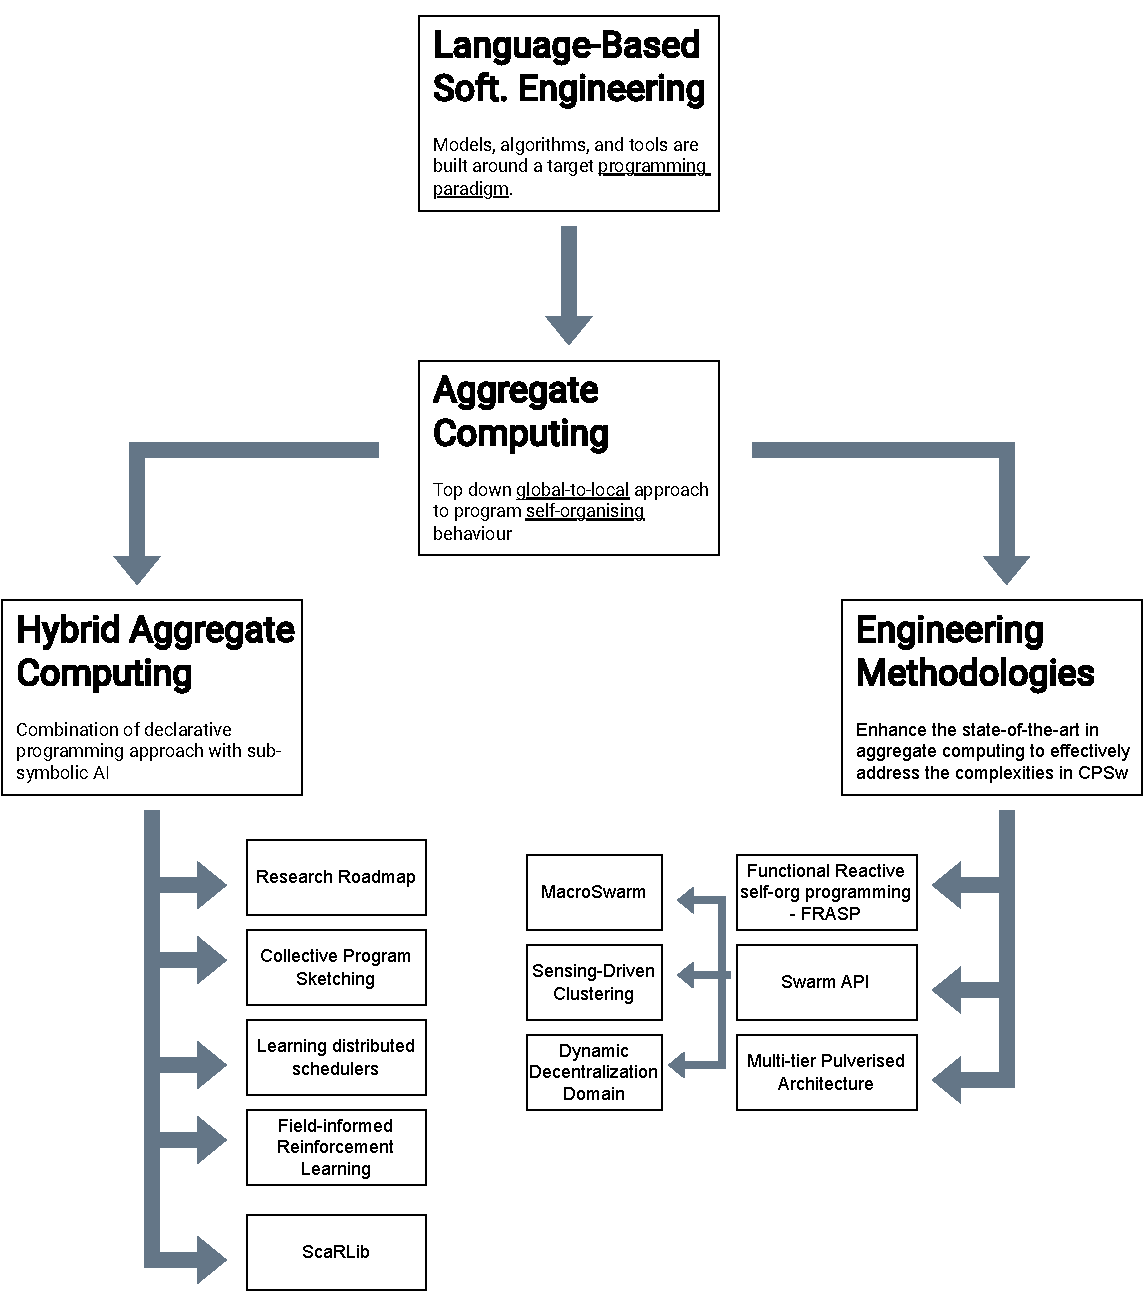
\includegraphics[width=\textwidth]{chapters/img/contribution-visual.drawio.pdf}
    \caption{Graphical overview of the thesis contributions.}
\end{figure}
\section{Thesis structure}
This thesis is organized as follows.

\Cref{chap:introduction} provides an overview of the research background and context, 
 and outlines the thesis structure and contributions.

\Cref{part:background} presents the theoretical foundations of this work.

\Cref{part:learning} introduces the contribution of the proposed hybrid approach for learning in \acp{cpsw}.

\Cref{part:engineering} discuss the contribution w.r.t. the engineering aspect of \acp{cpsw}.
\printbibliography[title=References]

\section{Publication List}


%%%%%%%%%%%%%%%%%%%%%%%%%%%%%%%%%%%%%%%%%%%%%%%%%%%%%%%%%%%%%%%%%%%%%%%%%%%%%%%%%%%%%%%%%%%%%%%%%%%%
%%%%%%%%%%%%%%%%%%%%%%%%%%%%%%% PART I %%%%%%%%%%%%%%%%%%%%%%%%%%%%%%%%%%%%%%%%%%%%%%%%%%%%%%%%%%%%
%%%%%%%%%%%%%%%%%%%%%%%%%%%%%%%%%%%%%%%%%%%%%%%%%%%%%%%%%%%%%%%%%%%%%%%%%%%%%%%%%%%%%%%%%%%%%%%%%%%% 

\part{Background}\label{part:background}
\begin{refsection}
%!TeX root = thesis-main.tex
\chapter{Cyber-Physical Swarms}\label{chap:cpsw}\mtcaddchapter
\minitoc% Creating an actual minitoc
The aim of this section is to elucidate the concept of \textit{Cyber-Physical Swarms}, 
 distinguish systems that align with our conceptual framework (an overview is given in \Cref{fig:overview-cpsw}), 
 and identify research domains grappling with analogous challenges. 
% 
\begin{figure}
    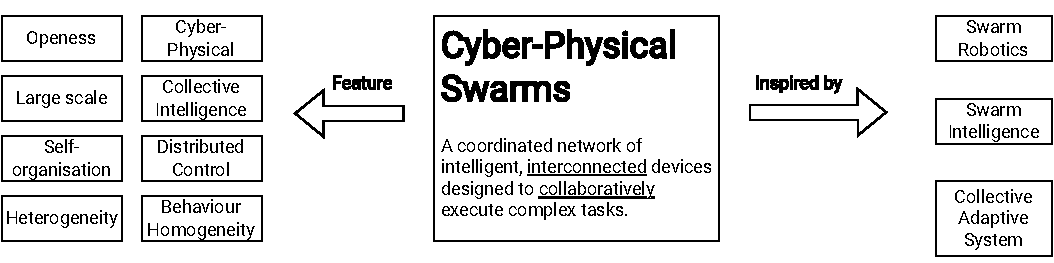
\includegraphics[width=\textwidth]{chapters/img/cyber-physical-swarms-overview.drawio.pdf}
    \caption{Overview of \acf{cpsw} and its related concepts}\label{fig:overview-cpsw}
\end{figure}
\section{Overview}
The term refers to a network of computational nodes working in concert to address collective problems, 
 akin to naturally occurring swarm phenomena ---in the following will be also referred to as ``swarm'' systems or ``swarm-like'' systems.
%
The architecture of these systems comprises a large array of interconnected nodes, 
 numbering in the hundreds or thousands. 
% 
Importantly, these networks are \textit{open}, 
 implying that the total node count is not predetermined. 
% 
As a result, 
 the emergent collective behaviour should exhibit \textit{scale-independence}, 
 ensuring that the same programmatic logic applies across small and expansive networks alike.
%
In these systems, each node is tethered to a \textit{physical} entity through sensors and can influence its environment via actuators. 
 This integration of computational and physical elements justifies the term ``cyber-physical''. 
 The nodes may exhibit heterogeneity in hardware or other attributes, 
 yet they maintain a \emph{homogeneous} local behaviour, executing identical local algorithms.
%
Nodes operate with a focus on collective goals, 
 as opposed to individualistic or selfish objectives, 
 thereby adhering to a collaborative ethos.
%
However, each node can still have local objectives, 
 which are not necessarily aligned with the global ones.
% 
Given that centralization is not feasible, 
 the architecture relies on distributed control mechanisms. 
 While modern computing paradigms such as cloud or edge infrastructures are applicable, 
 it is imperative that the system be capable of swift local responses. 
 This is especially critical given that these are often \emph{critical systems}, 
 where delays in decision-making could have severe repercussions.

In concluding, 
 it is pertinent to clarify that the focus of this study is on the \textit{macro-level} behaviours of the swarm, 
 rather than the \textit{micro-level} interactions. 
 Rather than characterizing the collective through emergent properties, 
 the intention is to define a \emph{globally} desirable structure.

%As for related concepts, 
% \acp{cpsw} can be considered a subset of Complex Adaptive Systems~\cite{holland1992complex}. 
% However, our framework imposes additional conditions not universally found in standard definitions of complex systems, 
% such as many collaborative agents.
% 
%Collective Adaptive Systems~\cite{DBLP:journals/corr/abs-1108-5643} closely resemble our definition of \acp{cpsw}, 
% but they diverge in that agents in our framework are geared toward \emph{collective} goals 
% and exhibit homogeneous behaviour.

In the subsequent section, 
 the concept of \acp{cpsw} will be elucidated through a range of examples. 
 These will encompass both existing and prospective applications to provide a comprehensive understanding of the field.
\section{Vision examples}\label{chap:cpsw:vision}
\subsection{Wild-fire monitoring in extensive forests}
Canada is renowned for its lush forests, 
 which cover approximately one-third of the nation's landmass, 
 making it one of the countries with the largest forested areas globally. 
These green expanses are not only a source of natural beauty but also play a crucial role in maintaining ecological balance. 
 However, the increasing impact of climate change has led to a surge in wildfires, 
 causing widespread devastation to both local flora and fauna.
 Consider for instance the 2023 wildfires, 
 which burned over 43 million acres, 
 that is about 5\% of the entire forest area of Canada~\cite{enwiki:1178342069}. 

To address this pressing issue, 
 there is a growing consensus on the need for proactive and localized interventions. 
 Specialized monitoring systems are essential for keeping tabs on vulnerable regions, 
 especially given the impracticality of relying solely on human observation due to the vastness of these areas. 
 One innovative solution might be the deployment of a sophisticated network of environmental sensors, strategically placed to monitor temperature, humidity, and other fire-prone conditions. 
 These sensors might be complemented by a swarm of drones equipped with advanced imaging and data collection capabilities.

The system operates through ongoing collaboration between ground-based sensors and aerial drones. 
 The drones provide a bird's-eye view of the landscape, 
 allowing for real-time monitoring of a wide array of nodes across large geographical expanses. 
 This integrated approach enables the early detection of potential fire hazards, 
 thereby facilitating the pre-emptive mobilization of emergency services.

However, the implementation of such a comprehensive monitoring system comes with its own set of challenges. 
 Each sensor or drone has a limited operational range and can only provide a \emph{partial} view of the overall system. 
 Therefore, robust data fusion algorithms are necessary to merge information from multiple sources into a cohesive and actionable overview. 
 Environmental conditions are also highly dynamic, requiring the system to \emph{adapt} in real-time to changing variables such as wind speed, temperature fluctuations, and precipitation levels.

In specific regions where the risk is elevated
 ---such as areas with active fires or reduced visibility due to smoke or fog---there may be a need for deploying additional sensors and drones. 
 Given that drones have limited battery life and need to be recharged, 
 the system must be capable of \emph{self-organizing} to ensure uninterrupted monitoring. 
 This is particularly challenging considering that the number of deployed devices could easily exceed thousands of units across the extensive area of interest.

Moreover, the system must be highly responsive to emergency conditions. 
 This necessitates that each device, whether a sensor or a drone, 
 should be equipped with \emph{edge computing} capabilities for performing local analyses. 
 These local analyses can then be used to trigger collective alarms, 
 ensuring immediate action is taken to mitigate the risk of wildfires.
\subsection{Crowd steering}
Concert venues (or public event like soccer matches) 
 are often filled with an energetic and enthusiastic crowd, 
 eager to enjoy live performances. 
 These events can attract tens of thousands of attendees, 
 making crowd management a critical concern for both safety and enjoyment. 
% 
However, traditional methods of crowd control, 
 such as barriers and security personnel, 
 are increasingly proving to be inadequate in the face of evolving challenges like sudden surges or emergency situations. 
 Take, for example, the 2019 stampede at the San Carlo place in Turin, 
 where a sudden downpour led to chaotic movements among the crowd, 
 resulting in thousands minor injuries and three deaths~\cite{enwiki:1164182872}.

To address this complex issue, 
 there is a growing interest in leveraging technology for more effective crowd steering. 
 One promising approach might be to equip each attendee with \emph{smart} bracelets or utilize their smartphones, 
 both of which have computational capabilities. 
 These devices can communicate only with each other, 
 forming a dynamic and adaptive network.

The system functions through real-time data exchange 
 between the individual devices %and strategically placed sensors around the venue. 
 The individual smart devices provide a ``ground-level'' perspective, 
 allowing for a granular understanding of crowd behaviour.

This collaborative approach enables the system to identify potential issues before they escalate. 
 For instance, if a particular section of the venue becomes too crowded, 
 the system can send alerts or directions to the smart devices in that area, 
 advising attendees to move to less crowded sections. 
 This facilitates the proactive redistribution of the crowd, 
 thereby averting potential safety hazards.

However, implementing this advanced crowd-steering system is not without challenges. 
 Each smart device only has a \emph{limited} computational capacity 
 and can provide just a \emph{partial} view of the overall crowd dynamics. 
Therefore, sophisticated algorithms are needed to aggregate 
 this fragmented data into a comprehensive and actionable overview. 
 Additionally, the system must be able to \emph{adapt} rapidly to changing conditions, 
 such as sudden weather changes or unexpected incidents during the concert.

In specific situations where immediate action is required 
 -- such as medical emergencies or security threats -- 
 there may be a need to send targeted alerts or instructions to specific groups of attendees. 
 Given that smart devices have limited battery life, 
 the system must also \emph{self-organize} to prioritize critical alerts and instructions, 
 ensuring that crowd management remains effective throughout the event.

Moreover, the system must be highly responsive to real-time conditions. 
 This necessitates that each smart device should compute locally, 
 allowing for point-wise decision-making. 
 These local analyses can then trigger \emph{collective} actions, 
 such as coordinated movements or emergency evacuations, 
 ensuring that immediate and effective measures are taken to maintain crowd safety.

\subsection{Autonomous vehicles}
In a not-so-distant future
 where human-driven cars have become a thing of the past, 
 cities will be bustling with \emph{swarms} of autonomous vehicles. 
% 
These self-driving cars will revolutionize urban transportation, 
 offering a safer and more efficient means of getting from one place to another. 
Indeed, considering the current situation, 
 where the number of accidents and traffic jams is increasing (only in 2023, there were over 5 million accidents worldwide\footnote{\url{https://www.forbes.com/advisor/legal/car-accident-statistics/}}), 
 this is a very appealing scenario.

However, the complexity of managing these autonomous fleets is far from trivial, 
 especially during peak hours or special events. 
%
Take for example Tokyo,
 where on average it is estimated that
 over 1 million cars enter the metropolitan area every day\footnote{\url{https://www.statista.com/statistics/1191368/shutoko-average-daily-traffic-volume/}}.

To tackle this intricate challenge, 
 there is a growing emphasis on the need for advanced management systems capable 
 of steering these autonomous vehicles effectively. 
 Each vehicle will be equipped with powerful onboard computers 
 and an array of sensors, 
 enabling them to communicate not only with a centralized traffic management system 
 but also with each other.

The system will operate through continuous data 
 exchange between individual cars 
 and strategically located infrastructure sensors. 
 These sensors monitor various parameters such as traffic flow, 
 road conditions, and even weather. 
 Autonomous cars provide a ``street-level'' perspective, 
 allowing for real-time adjustments to routing algorithms 
 and speed controls.

This collaborative approach enables the system to pre-empt potential bottlenecks and accidents. 
 For instance, if a major sporting event ends, 
 causing a sudden influx of ride requests, 
 the system can dynamically reroute cars to manage the increased demand efficiently. 
 This proactive approach minimizes congestion and enhances overall traffic flow.

However, the deployment of such a sophisticated system is fraught with challenges. 
 Each autonomous car has a \emph{limited} sensor range and can only offer a \emph{partial} view of the overall traffic landscape. 
 Therefore, advanced machine learning algorithms are essential to integrate this fragmented data into a cohesive and actionable real-time model. 
 Additionally, the system must be capable of \emph{adapting} quickly to changing conditions, such as road closures, accidents, or even fluctuating demand patterns.

In specific scenarios where immediate action is required
 ---like emergency vehicle passage or sudden road closures---
 there may be a need to prioritize certain routes or vehicles. 
 Given that each car operates on a finite energy source, the system must \emph{self-organize} to ensure that cars with lower battery levels are routed to charging stations without disrupting the overall traffic flow.

\section{Characteristics}
Drawing from the overview and the diverse examples provided, 
 several distinct characteristics emerge that set \acp{cpsw} apart from other large-scale 
 distributed systems. 
% 
These unique traits not only define the essence of \acp{cpsw} but also pose specific challenges in their design and implementation. 
 Each of these characteristics will be discussed in detail below.

\paragraph*{Scale}
\acp{cpsw} are inherently scalable, 
 often comprising hundreds or even thousands of interconnected nodes. 
 The behaviour scale independence ensures that the same programmatic logic can be applied across networks of varying sizes, 
 making them highly adaptable to different application scenarios.
 In doing this, is essential to capture the right collective abstraction that 
 allows both to help the developers to think in terms of the collective behaviour
 and to effectively design the collective behaviour itself.

\paragraph*{Device Heterogeneity}
While the nodes in a \ac{cpsw} may possess varying hardware capabilities and attributes, they are engineered to operate cohesively. Interoperability stands as a fundamental requirement for these systems, particularly because they often incorporate a diverse array of devices manufactured by different vendors. In today's Internet of Things (IoT) landscape, semantic interoperability presents a significant challenge. Devices from various vendors might employ divergent communication protocols or data formats, complicating the task of achieving seamless interaction. This heterogeneity isn't limited to communication protocols; it also extends to computational power, sensor types, and other attributes. Such diversity introduces an additional layer of complexity in system design, necessitating the identification of a common framework that enables effective communication and collaboration among the devices.
\paragraph*{Behaviour Homogeneity}
Despite the diverse hardware configurations, 
 nodes within a \ac{cpsw} display consistent behaviour at the local level.
 They run the same local \emph{algorithms}, thereby achieving the system's collective objectives in a standardized way. 
 However, it is important to clarify that ``homogeneous behaviour'' does not imply that all nodes do the same thing at the same time.
 Indeed, given the system's inherently distributed and potentially expansive nature, 
 the input received by one node may differ from that of another, 
 leading to variations in local behaviour.

\paragraph*{Distributed Control}
Centralized control mechanisms are often impractical in \acp{cpsw} due to their scale and complexity. 
 As a result, these systems rely on distributed control algorithms that enable nodes to make local decisions that collectively contribute to global objectives.

\paragraph*{Self-organization}
One feature of \acp{cpsw} is their ability to self-organize. 
Nodes can dynamically adapt to changing conditions, reconfiguring themselves to maintain system integrity and performance. 
This is particularly important in scenarios where the environment is unpredictable or hostile.

\paragraph*{Openness}
\acp{cpsw} are typically open systems, meaning that the total node count is not predetermined. 
New nodes can join or leave the network dynamically, requiring the system to be flexible enough to accommodate these changes without compromising its functionality.

\paragraph*{Collective Intelligence}
The nodes in a \ac{cpsw} work collaboratively to achieve common goals, displaying a form of collective intelligence. 
This is facilitated by advanced algorithms that enable the system to learn from its environment and adapt its behaviour accordingly.

\paragraph*{Cyber-physical Interactions}
The term ``cyber-physical'' aptly describes the integration of computational and physical elements in \acp{cpsw}. 
 Each node is usually connected to a physical entity via sensors and can influence its environment through actuators. 
 This seamless integration is crucial for applications that require real-time interaction with the physical world.

\section{Related concepts}
\begin{table}[h]
    \centering
    \resizebox{\textwidth}{!}{%
    \begin{tabular}{|c|c|c|c|c|}
    \hline
                                & MAS                         & Swarm Robotics          & CAS          & \ac{cpsw}         \\ \hline
    Scale                       & Dozens                      & Hundreds                & Thousands    & Thousands    \\ \hline
    Capabilities                & Heterogenous                & Homogenous              & Heterogenous & Heterogenous \\ \hline
    Behaviours                  & Heterogenous                & Homogenous              & Heterogenous & Homogenous   \\ \hline
    Control                     & Centralized/Distributed     & Centralized/Distributed & Distributed  & Distributed  \\ \hline
    Cyber-Physical              & Yes/No    & Yes & Yes/No  & Yes  \\ \hline
    \end{tabular}%
    }
    \caption{Summarized comparison between MAS, Swarm Robotics, CAS and \ac{cpsw}}
    \label{table:your_label}
\end{table}
This section will discuss some of the related concepts that are closely aligned with \acp{cpsw} summarized in \Cref{fig:overview-cpsw-taxonomy}.
\begin{figure}
    \centering
    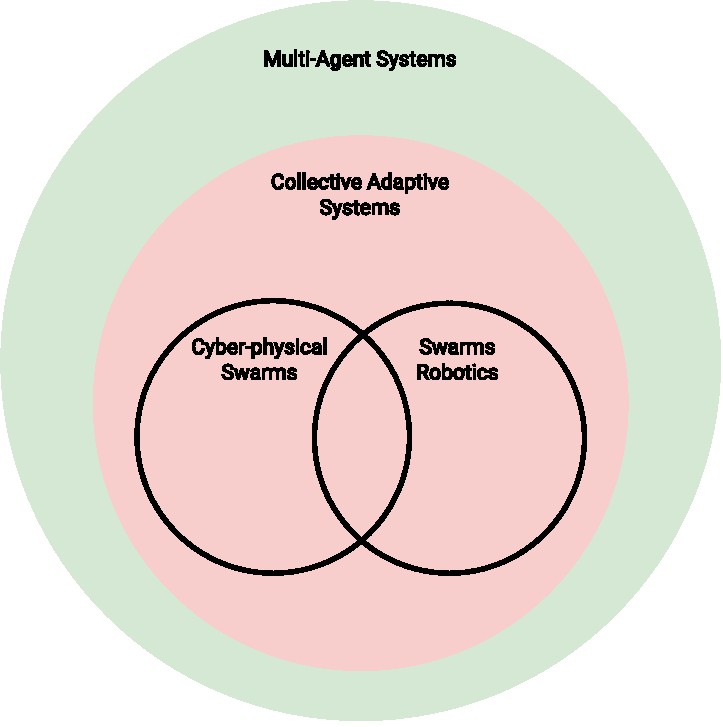
\includegraphics[width=0.6\textwidth]{chapters/img/cyber-physical-swarms-taxonomy.drawio.pdf}
    \caption{Taxonomy of \acf{cpsw} w.r.t related Systems}\label{fig:overview-cpsw-taxonomy}
\end{figure}
%% TODO: add more context of MAS system? gerarchy, organisation, etc.
\paragraph*{Multi-Agent Systems}
In the realm of computational systems, a \ac{cpsw} can be closely related to a Multi-Agent System (MAS), 
 with a specific emphasis on being a \emph{many}-agent system. 
 In a MAS, multiple autonomous agents interact with each other to achieve specific objectives. 
 These agents are capable of sensing their environment, making decisions based on their observations, and then acting upon those decisions. 
 The key difference in a \ac{cpsw} is the scale and the integration of physical components, such as sensors and actuators, which allows for real-time interaction with the environment.

In a \ac{cpsw}, agents are not just virtual entities but are tethered to physical components, making them cyber-physical agents. 
 These agents continuously engage in a cycle of \emph{repeated} sensing, computation, communication, and actuation to achieve collective behaviours. 

One of the significant challenges in designing a \ac{cpsw} is the high stochastic of the environment. 
 Unlike controlled settings where outcomes can be predicted with a high degree of accuracy, \acp{cpsw} often operate in dynamic and unpredictable environments. 
 This makes it nearly impossible to pre-program optimal behaviours for all agents. 
 The agents must, therefore, be capable of adapting their behaviours in real-time based on their sensory inputs and the inputs from other agents in the network. 
 This requires sophisticated algorithms that can handle uncertainty and make near-optimal decisions in real-time.

Moreover, the agents in a \ac{cpsw} are designed to work collaboratively to achieve collective goals, 
 rather than pursuing individual objectives. 
 This is in contrast to some MAS where agents might have conflicting goals. 
 In a \ac{cpsw}, the focus is on achieving a form of collective intelligence through distributed computing and decision-making. 
 Agents share information and coordinate their actions to solve complex problems that are beyond the capabilities of any single agent.

In summary, while \acp{cpsw} share similarities with MAS in terms of multi-agent interaction and decision-making, they extend the concept by incorporating large-scale, cyber-physical integration, and a focus on collective intelligence. 
 The challenges in designing \acp{cpsw} are manifold, ranging from handling the stochastic nature of the environment to ensuring robust and adaptive collective behaviours.

\paragraph*{Swarm intelligence} It is an interdisciplinary field that draws inspiration from the collective behaviours observed in social animals, 
 such as ants, birds, and fish, to develop computational algorithms and systems. 
 Initially, the focus was primarily on Swarm Robotics, 
 where the objective was to create robotic systems that could emulate the complex behaviours seen in natural swarms. 
 The methodology employed is fundamentally bottom-up. 
 Designers and researchers study the behaviours of individual animals in their natural habitats to understand the rules or heuristics they follow. 
 These individual behaviours are then modelled computationally to observe how they contribute to the emergence of collective intelligence in a swarm. 
 One seminal concept that emerged from this line of inquiry is \textit{stigmergy}~\cite{DBLP:journals/fgcs/DorigoBT00}. 
 Stigmergy is a form of indirect communication and coordination where agents in a swarm interact with each other by modifying a shared environment, rather than through direct communication.

In recent years, the focus of swarm intelligence has evolved to concentrate more on algorithmic aspects. 
 Researchers have started to leverage the principles of collective behaviour to develop optimization algorithms that can solve complex computational problems. 
 These algorithms are particularly useful in scenarios where traditional optimization methods are computationally expensive or fail to find optimal solutions within a reasonable time frame. 
 Some of the most well-known algorithms that have emerged from Swarm Intelligence research include Ant Colony Optimization (ACO)~\cite{DBLP:journals/tsmc/DorigoMC96}, Particle Swarm Optimization (PSO)~\cite{DBLP:conf/icnn/KennedyE95}, and Flock of Starling Optimization (FSO)~\cite{DBLP:series/sci/FulgineiS11}. 
Each of these algorithms has its own set of rules and heuristics, modelled after the specific animal behaviours they are inspired by, and they have been applied successfully in various domains such as network design, resource allocation, and data clustering.

While these optimization algorithms offer valuable methodologies and have broad applicability, they are not the central focus of this thesis. 
 Differently, the focus is on harnessing the \emph{principles} of Swarm Intelligence to develop \emph{artificial} systems that can achieve similar collective behaviours through mechanisms of \emph{self-organization}. 
 Unlike traditional Swarm Intelligence algorithms that often aim to \textit{mimic} nature, this thesis draws \textit{inspiration} from natural systems to understand the fundamental principles that make these systems \emph{robust}, \emph{scalable}, and \emph{adaptable}. 
 The ultimate goal is to exploit these principles to design and implement artificial swarm systems that can operate effectively and efficiently in complex, dynamic, and potentially hostile environments. 
 
\paragraph*{Swarm robotics}

Historically, 
 the field of swarm robotics has its roots in the early approaches to swarm intelligence. 
 Over time, it has evolved to become the \textit{engineering} arm of swarm intelligence, 
 focusing on the \emph{practical} aspects of building and maintaining swarm systems. 
 The overarching goal of \emph{swarm engineering} is to establish a rigorous methodology for the entire lifecycle of a swarm robotics system, 
 from conceptualization to operation and maintenance~\cite{DBLP:journals/swarm/BrambillaFBD13}.

In traditional Swarm Robotics, the primary focus is on \textit{robots} that are \emph{autonomous}, \emph{situated}, and operate under \emph{no central control}. 
 These robots are designed to interact with each other and their environment to achieve collective goals. 
 \ac{cpsw} extends this paradigm to include other ``swarm-like'' systems that may not necessarily involve robots. 
 Examples include crowds of people in public spaces, 
 large-scale IoT networks, and smart city infrastructures. 
 These systems share many similarities with swarm robotics, 
 such as the need for autonomy, 
 localized decision-making, 
 and collective behaviour, but they also present unique challenges and opportunities.

One of the most promising avenues for extending the principles of swarm robotics to these other domains is the emerging field of \textit{automatic design}~\cite{DBLP:journals/firai/FrancescaB16}. 
 In automatic design approaches, 
 the control logic for the agents in the swarm is not manually programmed but is instead derived through optimization techniques such as \textit{genetic algorithms} or \textit{Multi-agent Reinforcement Learning}.
These methods aim to optimize a \textit{global} utility function that captures the overall objectives of the swarm. 
 This is particularly appealing for \acp{cpsw}, 
 where the complexity and scale of the system make manual programming impractical.

In summary, 
 the principles and methodologies developed in swarm robotics provide a strong foundation for the engineering of \acp{cpsw}. 
 However, the unique challenges and complexities of \acp{cpsw} require further innovation. 
 By leveraging the principles of swarm intelligence,
 we can create a more robust, adaptable, and intelligent \acp{cpsw} that can operate effectively in a wide range of applications and environments.

\paragraph*{Collective Adaptive Systems}
Collective adaptive systems are a broad class of systems composed of agents 
 (potentially heterogeneous) capable of adapting to environmental conditions 
 while striving to achieve a collective goal through the emergence of individual node cooperation. 
%
Typically, individual units are simple and draw strong inspiration from natural systems. 
 In these systems, which are adaptive by nature, 
 there is interest in incorporating \emph{self-*} properties (in fact, these CAS are sometimes discussed as collective self-adaptive systems). 
%
These properties include \emph{self-healing}, \emph{self-optimization}, and \emph{self-configuration}. 
Self-healing refers to the system's ability to recover from failures without human intervention. 
Self-optimization means the system can improve its performance over time based on feedback. Self-configuration allows the system to adapt to changing conditions without requiring manual adjustments. 
These self-* properties contribute to the system's overall \emph{resilience} and \emph{efficiency}.

\ac{cpsw} can be understood as a specialized subset of the broader CAS.
This specialization arises from two key distinguishing characteristics:
i) The involved entities are not merely digital but also have a \emph{cyber-physical} nature,
 integrating both computational and physical elements.
ii) Despite the heterogeneous nature of the devices within the system, 
 their behaviour manifests uniformly.
These unique attributes have a profound impact on the system's design methodology, 
 which is why this thesis specifically focuses on this subclass of systems.
%
%\printbibliography

\section{Final Remarks}
\Acf{cpsw} represent a specialized subset of Collective Adaptive Systems (CAS), distinguished by their cyber-physical nature and homogeneous behaviour despite device heterogeneity. 
 Drawing from the principles of swarm intelligence, multi-agent systems, and swarm robotics, 
 \ac{cpsw} offer a promising avenue for tackling complex, large-scale problems in a variety of domains, from environmental monitoring to crowd management and autonomous transportation.

The unique characteristics of \ac{cpsw}, such as scale, 
device heterogeneity, behaviour homogeneity, and self-organization, not only define their essence but also pose specific challenges and opportunities in their design and implementation. 
These challenges necessitate innovative approaches in automatic design,
 distributed control, and self-organization.

This thesis aims to contribute to the understanding and engineering of \ac{cpsw} by exploring these challenges and proposing methodologies that leverage the principles of collective behaviour to design systems that are robust, scalable, and adaptable. 

\chapter{Macro-programming}\label{chap:macro-programming}

%!TeX root = thesis-main.tex
\chapter{Reinforcement Learning}\label{chap:marl}

\minitoc% Creating an actual minitoc
\newcommand{\RS}{\mathcal{S}}
\newcommand{\RA}{\mathcal{A}}
\newcommand{\RP}{\mathcal{P}}
\newcommand{\RR}{\mathcal{R}}
\newcommand{\RE}{\mathbb{E}}

The concept of intelligence is as complex as it is intriguing, 
 and it has been a subject of philosophical inquiry, 
 scientific exploration, and cultural curiosity for centuries. 
 Philosophers have debated on what constitutes intelligence, 
 linking it to \emph{reason}, \emph{wisdom}, and even \emph{morality}. 
%
Despite these varied interpretations, 
 defining intelligence remains a challenge, 
 even in the field of psychology. 
%
Several standardized tests and scales attempt to measure intelligence,
 like the one developed by Alan Turing~\cite{Turing1950-TURCMA}, 
 but none manage to capture the complete essence of what it means to be ``intelligent''. 
 Intelligence is often understood as the ability to \emph{learn}, \emph{reason}, and \emph{adapt}, among other cognitive abilities.

Among the myriad of perspectives on intelligence, learning stands out as a \emph{fundamental} component. 
 From an evolutionary point of view, 
 the ability to learn is essential for survival. 
 An organism that can adapt to its environment and learn from experiences is likely to survive and reproduce. 
 In the human context, learning has been the cornerstone of development, be it mastering a language, solving complex problems, or creating art.

This notion of learning is crucial in the realm of Artificial Intelligence (AI). 
%
 If intelligence involves learning, 
 then replicating intelligence artificially would necessarily entail enabling machines to learn. 
 This hypothesis leads us to the exciting and rapidly evolving domain of \emph{machine learning}---
 a subset of AI that allows computers to learn from data, 
 rather than requiring them to be explicitly programmed for specific tasks.

Machine learning is not monolithic; 
 it encompasses various approaches and techniques that aim to make machines learn. 
 Broadly, these approaches can be categorized into supervised learning, unsupervised learning, semi-supervised learning, and reinforcement learning.
%
Particularly, the first three approaches are based on the idea of learning from data, 
 where the data is either labelled or unlabelled:
\begin{itemize}
  \item \emph{supervised learning}: this is the most straightforward approach, where a model is trained on a labelled dataset. 
  The model makes predictions or decisions based on input data and is corrected when its predictions are incorrect. Typical examples include classification and regression problems;
  \item \emph{unsupervised learning}: unlike supervised learning, this approach does not involve labelled data. 
  The machine tries to learn the patterns and the structure from the data without any supervision (e.g., clustering algorithms);
  \item \emph{semi-supervised}: A middle-ground between supervised and unsupervised learning, this approach utilizes both labelled and unlabelled data for training. The model learns to improve its predictions gradually.
\end{itemize}
Reinforcement learning sets itself apart from other methodologies by operating without the need for labelled data or supervision and through a sequential decision. 
 It employs a \emph{trial-and-error} strategy, mirroring the way humans acquire knowledge. 
 Subsequent sections will delve into the nuances of this distinctive approach, starting from single agent settings and then moving to multi-agent and many-agent systems---the focus of this thesis.
\section{Single-agent}\label{chap:rl:single}
\begin{figure}
  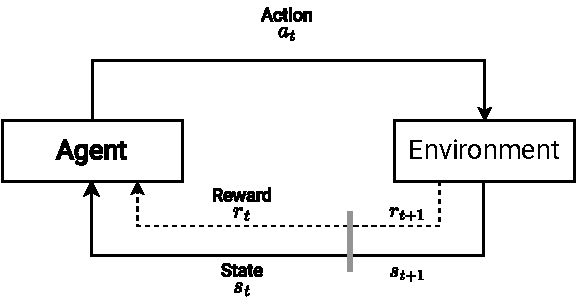
\includegraphics[width=\textwidth]{chapters/img/single-agent-rl.drawio.pdf}
  \caption{Overview of the \ac{rl} framework.}\label{fig:rl:overview}
\end{figure}
\Acl{rl}~\cite{sutton2018reinforcement-learning} serves as a universal framework that h
 as been inspired by the cognitive processes underlying human learning. 
 This paradigm has proven to be highly effective for addressing \emph{control problems}, 
 which are essentially tasks that require decision-making to achieve a particular outcome.
%
The core focus of \ac{rl} is on the \emph{sequential} interactions that occur between \emph{agents} 
 and an \emph{environment} (summarized in \Cref{fig:rl:overview}). 
 Agents are defined as entities capable of performing \emph{actions}, 
 while the environment constitutes everything that is external to the agents 
 and beyond their immediate control.

During each discrete time step, 
 denoted as $t$, an agent observes the current state of the environment, 
 $s_t$ (e.g., the robot position according to a GPS sensor). 
This state encapsulates the set of all observable information at that particular moment. 
The agent then proceeds to select an \emph{action} 
 (e.g., the torque to be applied to engines) 
 $a_t$ in accordance with its \emph{policy} $\pi$. 
A policy serves as a probabilistic mapping that guides the agent in choosing actions 
 based on the current state. 
 Policies can be simple lookup tables or complex neural networks.

As a result of taking this action, 
 the environment transitions to a new state $s_{t+1}$ at the next time step $t+1$. 
 Simultaneously, the agent receives a \emph{reward} $r_{t+1}$, 
 which is a quantitative measure of the efficacy of the action taken, 
 given the state of the environment.

The overarching objective of \ac{rl} is to discover an \emph{optimal} policy, 
 denoted as $\pi^*$, that aims to maximize the long-term return, or cumulative reward, $G$. 
 This is generally achieved through a \emph{trial-and-error} learning process, 
 where agents continually adapt their policies based on the rewards received.

This framework has found extensive applications in a diverse array of domains. 
 For example, \ac{rl} has been used to create advanced algorithms for video games~\cite{DBLP:journals/spm/ArulkumaranDBB17}, 
 allowing for AI agents that can outperform human players. 
% 
In robotics~\cite{DBLP:journals/ijrr/KoberBP13}, 
 \ac{rl} algorithms are enabling machines to learn complex tasks autonomously, 
 from simple object manipulation to navigation in unstructured environments. 
 It is also making significant inroads in networking, 
 particularly in routing algorithms where dynamic decision-making is crucial~\cite{DBLP:journals/comsur/LuongHGNWLK19}.

\subsection{Markov Decision Process}
This general framework is supported by \ac{mdp}, 
 a mathematical model that describes the environment evolution in sequential decision problems. 
%
A \ac{mdp} consists of a tuple $<\RS, \RA, \RP, \RR>$ in which:
\begin{itemize}
  \item $\RS$ denotes the set of states;
  \item $\RA$ is the set of actions;
  \item $\RP(s_{t + 1} | s_t, a_t)$ define the probability to reach some state $s_{t + 1}$ starting from $s_t$ and performing $a_t$ (i.e. transition probability function);
  \item $\RR(s_t, a_t, s_{t+1})$ devise a probabilistic reward function.
\end{itemize}
In \ac{mdp}, $\RP$ is \emph{memory-less}, 
 namely the next environment state depends only on the current state---
 that is the \emph{Markov property}.
%%
%Typically, in \ac{rl} problems, agents do not have access to $\RR$ or $\RP$, 
% but they can rely only on the experience $(s_t, a_t, r_t)$ sampled at a time step. 
%%
Another important concept in \ac{mdp} is the return 
 $G$ defined as the discounted sum of reward a possible future trajectory $\tau$ (i.e. a sequence of time steps):
%%
\begin{equation}
G_{t} = r_t + \gamma r_{t + 1} + \gamma^2 r_{t + 2} + \dots + \gamma^T r_{t + T} = \sum_{k = t}^T \gamma^{k-t} r_k
\end{equation}
%%
Where $0 \leq \gamma \leq 1$ is the \emph{discount factor}, 
 that is how much the future reward impacts the long-term return.
%%
Based on the value of $T$, we can distinguish between \emph{episodic} and \emph{continuous} tasks.
 The foster ones are characterized by a finite number of time steps
  (e.g., a match of chess), while the latter ones are infinite 
  (e.g., a robot that should wander in an unknown environment).
%%
\subsubsection*{Reinforcement Learning Goal}
The \ac{rl} goal can be expressed as the maximization of the \emph{expected} 
 long-term return following a policy $\pi$:
%%
\begin{equation}
J = \mathbb{E_\pi}\Big[ G_t \Big] = \RE_\pi \Big[ \sum_{k = t}^T \gamma^{t-k} r_k \Big] 
\end{equation}
%%
Particularly, in \ac{RL} we want to find the optimal policy $\pi^*$ that maximizes $J$:
%%
\begin{equation}
\pi^* = \arg \max_{\pi} J
\end{equation}
The equation essentially captures the trade-off between immediate and future rewards. 
 The agent aims to select actions based on the policy \(\pi\) 
 that will maximize this expected long-term return. 
 The discount factor \(\gamma\) allows us to model the agent's consideration 
 for future rewards and is a hyperparameter that can be tuned based on the specific problem being solved.

\subsection{Find a policy given a MDP}

$V^\pi$ is the value function that evaluates how good (or bad) a \emph{state} 
 is according to the long-term return following the policy $\pi$ (\emph{expected value}).
% 
It is defined as:
%%
\begin{equation}
V(s)^\pi = \RE_\pi \Big[ G_t | s_t = s \Big]
\end{equation}
%%
$Q^\pi$ is the corresponding value function that evaluates \emph{state-action} pairs:
%%
\begin{equation}
Q(s, a)^\pi = \RE_\pi \Big[ G_t | s_t = s, a_t = a \Big]
\end{equation}
Policies could be defined through value functions. 
 In particular, a greedy policy based on $Q$ function is the one that always chooses 
 the action with the highest value in a certain state:
\begin{equation}
\pi(s) = \arg \max_{a}(Q(s, a))
\end{equation}
\subsubsection{Dynamic programming}
\begin{figure}
  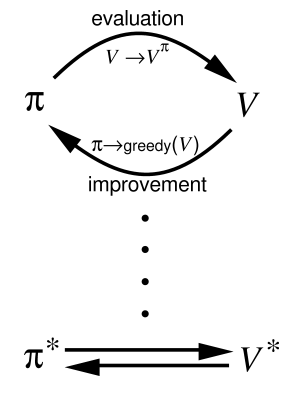
\includegraphics[width=0.3\textwidth]{chapters/img/generalized-policy-improvement.png}
  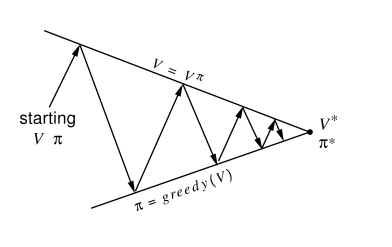
\includegraphics[width=0.65\textwidth]{chapters/img/value-iteration.png}
  \caption{General schema of policy iteration (left) and value iteration (right).}\label{fig:rl:dp}
\end{figure}
Dynamic programming is a family of algorithms that can be used to compute optimal policies 
 given a model of the environment as a \ac{mdp}.
%
In particular, the \emph{Bellman equation} is a fundamental concept in dynamic programming. 
 It is a recursive equation that decomposes the value function into two parts: 
 the immediate reward obtained from the current state and the discounted value of the future state. 
 The Bellman equation for the value function is defined as:
\begin{equation}
V(s) = \sum_{a \in \RA} \pi(a|s) \sum_{s' \in \RS} \RP(s'|s, a) \Big[ \RR(s, a, s') + \gamma V(s') \Big]
\end{equation}
%
Similarly, the Bellman equation for the $Q$ function is defined as:
\begin{equation}
Q(s, a) = \sum_{s' \in \RS} \RP(s'|s, a) \Big[ \RR(s, a, s') + \gamma \sum_{a' \in \RA} \pi(a'|s') Q(s', a') \Big]
\end{equation}
%
The Bellman equation is the basis for many algorithms that solve \ac{mdp},
two most notable are \emph{value iteration} and \emph{policy iteration} (\Cref{fig:rl:dp}).
\subsection{Value iteration}
Value iteration is an iterative algorithm used to compute the optimal value function \(V^*\) and, consequently, the optimal policy \(\pi^*\). 
 The algorithm is particularly useful when the state and action spaces are too large to solve directly through analytical methods. 
 It is based on the principle of optimality, which states that if an optimal policy \(\pi^*\) exists, then it must satisfy the Bellman optimality equation.

The algorithm starts by initializing \(V(s)\) for all states \(s\) to some arbitrary values, often zeros. 
 It then iteratively updates the value of each state \(s\) using the Bellman optimality equation until the value function converges to \(V^*\). 
 The convergence is usually checked by measuring the difference between successive value functions and comparing it against a small threshold \(\epsilon\):
\begin{equation}
V_{k+1}(s) = \max_{a \in \mathcal{A}} \sum_{s' \in \mathcal{S}} \RP(s'|s, a) \Big[ \RR(s, a, s') + \gamma V_k(s') \Big]
\end{equation}

The \(\max\) operation ensures that the value function is updated to reflect the best possible action at each state. 
 The term \(\gamma V_k(s')\) represents the discounted future rewards, and \(R(s, a, s')\) is the immediate reward. 
 The transition probability \(P(s'|s, a)\) models the uncertainty in the environment.

After the value function has converged to \(V^*\), the optimal policy \(\pi^*\) can be extracted. The policy is determined by selecting the action that maximizes the expected return in each state, as given by:

\begin{equation}
\pi^*(s) = \arg \max_{a} \sum_{s' \in \mathcal{S}} P(s'|s, a) \Big[ R(s, a, s') + \gamma V^*(s') \Big]
\end{equation}
This policy is guaranteed to be optimal with respect to the original MDP.


\subsection{Policy Iteration}
Policy iteration is another dynamic programming algorithm used for finding the optimal policy \(\pi^*\). 
 Unlike value iteration, policy iteration consists of two main steps: 
 \emph{policy evaluation} and \emph{policy improvement}, 
 which are repeated iteratively until the policy converges to \(\pi^*\):
\begin{itemize}
  \item policy evaluation: in this step, the value function \(V^\pi\) for the current policy \(\pi\) is computed until it stabilizes. The update rule is:

  \begin{equation}
  V_{k+1}(s) = \sum_{a \in \mathcal{A}} \pi(a|s) \sum_{s' \in \mathcal{S}} P(s'|s, a) \Big[ R(s, a, s') + \gamma V_k(s') \Big]
  \end{equation}
  \item policy improvement: after evaluating \(V^\pi\), the policy is updated to be greedy with respect to \(V^\pi\):
  \begin{equation}
  \pi'(s) = \arg \max_{a} \sum_{s' \in \mathcal{S}} P(s'|s, a) \Big[ R(s, a, s') + \gamma V^\pi(s') \Big]
  \end{equation}
\end{itemize}
The algorithm then returns to the policy evaluation step, using the new policy \(\pi'\), and continues until the policy no longer changes.
 
%The objective in value-based methods is to find the best value function (whether $Q$ or $V$), defined as:
%\begin{iequation}
%Q^* = \arg \max_{\pi}(Q^\pi(s, a)) \; \text{or} \; V^* = \arg \max_{\pi}(V^\pi(s))
%\end{iequation}
%Consequently, when we have found $Q^*$, an optimal policy is straightforwardly defined:
%\begin{equation}
%\pi^*(s) = \underset{a}{\text{argmax}}(Q^*(s, a))
%\end{equation}
\subsection{Find a policy without an MDP}
While dynamic programming methods like value iteration and policy iteration offer powerful ways to find the optimal policy \(\pi^*\), 
 they come with a significant limitation: 
 the need for a complete model of the environment. 
 Specifically, these algorithms require knowledge of the transition probability function \(\RP\) and the reward function \(\RR\). 
 In many real-world applications, these functions are either unknown or too complex to model accurately. 
 This is where \emph{model-free} algorithms come into play.
 In the following sections, we will discuss two such algorithms' family: 
 Monte Carlo methods and Temporal Difference methods.
\subsubsection{Monte Carlo methods}
Monte Carlo methods offer a way to find an optimal policy \(\pi^*\) without requiring a model of the environment. 
 These methods rely on sampling sequences of states, actions, and rewards from actual or simulated interactions with the environment. 
 By averaging these samples, the agent can estimate the value functions \(V(s)\) and \(Q(s, a)\), which can then be used to improve the policy.

The core idea is to run multiple episodes, 
 from start to finish, and then update the value estimates based on the returns observed. 
 The value of a state \(s\) or a state-action pair \((s, a)\) is estimated as the average of the returns that have followed that state or state-action pair across multiple episodes.

\begin{equation}
V(s) = \frac{1}{N} \sum_{i=1}^{N} G_t^{(i)}
\end{equation}

\begin{equation}
Q(s, a) = \frac{1}{N} \sum_{i=1}^{N} G_t^{(i)}
\end{equation}

Where \(N\) is the number of times the state or state-action pair has been visited, and \(G_t^{(i)}\) is the return following the \(i\)-th visit.

Once the value functions are estimated, 
 the policy can be improved by making it greedy with respect to these estimated values. 
%
In this context, the \emph{exploration-exploitation} trade-off is crucial.
%
In fact, the agent should explore the environment to discover new states and actions that could lead to higher rewards,
  but it should also exploit the knowledge it has already acquired to maximize the expected return.
%
Monte Carlo methods are particularly useful when the state and action spaces are large, making it impractical to enumerate all possible state-action pairs. However, they do require the episodes to be finite and can be computationally expensive due to the need for multiple samples to obtain accurate estimates.

\paragraph*{Exploration-Exploration dilemma}
In these algorithms, the agent should explore the environment to discover new states and actions that could lead to higher rewards,
  but it should also exploit the knowledge it has already acquired to maximize the expected return.
  This is the so-called \emph{exploration-exploitation} trade-off.
  This is not only a matter in Monte Carlo methods, but it is a general problem in model-free algorithms, in which agent should learn a policy without a model of the environment.
%
There are several ways to address this dilemma, 
 but the most common approach is to use an \emph{$\epsilon$-greedy} policy. 
 This policy selects a random action with probability \(\epsilon\) and the greedy action with probability \(1 - \epsilon\). 
 The value of \(\epsilon\) is typically set to a small value, 
 such as 0.1 or 0.2, 
 to ensure that the agent explores the environment sufficiently.
%

\subsubsection{Temporal difference methods}
Temporal difference methods are a class of \emph{model-free} and \emph{value-based} algorithms 
 that allow the agent to learn optimal behaviour directly from its interactions with the environment, without requiring a model. 
 TD methods combine ideas from both Monte Carlo methods and dynamic programming to provide a flexible and powerful approach to reinforcement learning.

One of the simplest TD methods is \emph{TD-Learning}~\cite{DBLP:journals/ml/Sutton88}, 
 which updates the value function \(V(s)\) based on the temporal difference error \(\delta\), 
 defined as \( \delta = R(s, a, s') + \gamma V(s') - V(s) \). 
 The value function is then updated using \( V(s) \leftarrow V(s) + \alpha \delta \), where \(\alpha\) is the learning rate.

Starting from this intuition two main approaches have been developed: 
 \emph{Q-learning}~\cite{DBLP:journals/ml/WatkinsD92} and \emph{SARSA}~\cite{10.5555/3312046}. 

 \paragraph*{Q-Learning}

 Q-Learning is an off-policy TD algorithm that focuses on learning the action-value function \(Q(s, a)\). The update rule for Q-Learning is:
 \begin{equation}
 Q(s, a) \leftarrow Q(s, a) + \alpha \Big[ R(s, a, s') + \gamma \max_{a'} Q(s', a') - Q(s, a) \Big]
 \end{equation}
 The algorithm is termed ``off-policy'' because it learns the value of the optimal policy regardless of the policy being followed, 
  thanks to the \(\max_{a'}\) term in the update rule.
 
 \paragraph*{SARSA}
 SARSA (State-Action-Reward-State-Action) is an on-policy TD algorithm. 
  Unlike Q-Learning, SARSA takes into account the current policy \(\pi\) during the learning process. The update rule for SARSA is:
 \begin{equation}
 Q(s, a) \leftarrow Q(s, a) + \alpha \Big[ R(s, a, s') + \gamma Q(s', a') - Q(s, a) \Big]
 \end{equation}
 where \(a'\) is the action taken under the current policy \(\pi\).
 
 Both Q-Learning and SARSA have their own advantages and disadvantages. 
  Q-Learning tends to find the optimal policy faster but may be more sensitive to noise. SARSA, being an on-policy method, is more conservative and tends to find safer policies, especially when the policy involves some level of risk or uncertainty.

\subsection{Policy Gradient Methods}

While temporal difference methods and monte carlo methods focus on learning value functions to derive optimal policies, \emph{policy gradient} methods take a different approach. 
  They aim to directly optimize the policy \(\pi\) itself, 
  rather than first estimating value functions. 
  This is particularly useful in environments with high-dimensional action spaces or continuous action spaces, where value-based methods may struggle.
  Moreover, in this way, it is possible to learn stochastic policies,
    which are often more robust and flexible than deterministic policies.

Policy gradient methods optimize the policy by ascending the gradient of the expected return with respect to the policy parameters \(\theta\). 
Mathematically, this can be expressed as:
\begin{equation}
\theta \leftarrow \theta + \alpha \nabla_\theta J(\theta)
\end{equation}
where \(J(\theta)\) is the expected return when following policy \(\pi_\theta\), and \(\alpha\) is the learning rate.

One of the foundational algorithms in this category is the REINFORCE algorithm~\cite{DBLP:conf/nips/SuttonMSM99}: it is one of the earliest and most straightforward policy gradient methods. 
It estimates the gradient of the expected return by sampling trajectories from the current policy \(\pi_\theta\). 
After each episode, the algorithm adjusts the policy parameters \(\theta\) in the direction that increases the expected return.
%
The core equation for the REINFORCE algorithm is:
\begin{equation}
\nabla_\theta J(\theta) = \mathbb{E}_{\tau \sim \pi_\theta} \left[ \sum_{t=0}^{\infty} \nabla_\theta \log \pi_\theta(a_t | s_t) G_t \right]
\end{equation}

Here, \(\tau\) represents a trajectory sampled from the policy \(\pi_\theta\), and \(G_t\) is the return from time \(t\). 
 The term \(\nabla_\theta \log \pi_\theta(a_t | s_t)\) is the log-likelihood gradient, 
 and \(G_t\) serves as a sample estimate for how good the action \(a_t\) is in state \(s_t\).

The REINFORCE algorithm operates in an episodic setting, 
 meaning it waits until the end of each episode to update the policy. 
 This makes it well-suited for tasks where the episode termination is natural, such as games or tasks with a fixed time horizon.
 REINFORCE is particularly useful when the action space is high-dimensional or continuous, where traditional value-based methods like Q-Learning may struggle.  
 However, one drawback of REINFORCE is that it can have high variance in its updates, which can make the training process unstable. 
 Various techniques, such as using a \emph{baseline} or employing advanced variance reduction methods, have been developed to mitigate this issue.
 Particularly, the \emph{actor-critic} architecture is a popular approach that combines the advantages of both value-based and policy-based methods.
 In this paradigm, the policy is referred to as the \emph{actor}, while the value function is referred to as the \emph{critic}.
The actor is responsible for selecting actions, while the critic evaluates the actions taken by the actor.

\subsection{Approximate Solutions}

While the fundamental algorithms discussed in previous sections provide a strong theoretical foundation for model-free RL, 
 they often fall short in real-world applications. 
 The primary challenges they face are:

\begin{itemize}
  \item \textbf{Curse of dimensionality}: The state and action spaces in practical problems can be so large that enumerating them becomes computationally infeasible.
  \item \textbf{Partial observability}: In many scenarios, the agent cannot fully observe the entire state of the environment, 
  making it difficult to make optimal decisions.
\end{itemize}
To illustrate the curse of dimensionality, 
 consider the seemingly simple game of Go. 
 The game's state space consists of \(2^{170}\) possible states, 
 a number so astronomical that it exceeds computational capabilities—especially when compared to the estimated \(10^{80}\) atoms in the observable universe.

Similarly, partial observability is a pervasive issue in real-world applications. 
 For example, a self-driving car perceives its environment through sensors, 
 offering only a limited, partial view of the world. 
 This restricted perspective can significantly impact the agent's ability to make optimal decisions.

Given these challenges, approximate solutions become not just desirable but often necessary. 
 These solutions leverage function approximation techniques to estimate value functions or policies. 
 While they may sacrifice some theoretical convergence guarantees, 
 they offer a more practical approach to tackling complex, high-dimensional, and partially observable problems commonly encountered in real-world applications.
%
In contemporary applications, neural networks have emerged as the go-to function approximators due to their exceptional capability to approximate complex, 
 high-dimensional functions. 
 Particularly, the combination of Deep learning and Reinforcement learning has led to significant advancements in the field, in the so-called area of \emph{deep reinforcement learning}.
 One of the first and most influential works in this area was the Deep Q-Network (DQN) algorithm~\cite{DBLP:journals/corr/MnihKSGAWR13}, that will be discussed in the next section.
 \subsubsection{Deep Q-Networks (DQN)}

 Deep Q-Networks (DQN) represent a landmark innovation in the field of deep reinforcement learning, 
  effectively combining the strengths of Q-Learning with the function approximation capabilities of deep neural networks.
  DQN was initially designed to master a variety of Atari 2600 games and has since been adapted for various complex tasks.
 
 The core idea behind DQN is to use a neural network as a function approximate for the Q-function in Q-Learning. 
  The neural network, often referred to as the Q-network, 
  takes the environment state as input and outputs Q-values for each action.
%  
Mathematically, the Q-network aims to approximate the optimal Q-function \(Q^*(s, a)\) 
 as closely as possible.
\begin{equation}
Q(s, a; \theta) \approx Q^*(s, a)
\end{equation}
 
where \(\theta\) represents the parameters of the neural network.
 
However, directly applying neural networks to Q-Learning presents challenges, 
 primarily due to the correlation between consecutive experiences and the non-stationary nature of the data. 
 DQN addresses these issues through two key innovations:
 
\begin{itemize}
  \item \textbf{Experience Replay}: DQN stores past experiences \((s, a, r, s')\) in a replay buffer and samples mini-batches randomly during training. 
  This decorrelates the data and leads to more stable training.
  \item \textbf{Target Network}: DQN introduces a separate, 
  slowly-updated target network to calculate the target Q-values, 
  reducing the overestimation bias and improving stability.
\end{itemize}
 
The Q-value update equation in DQN is:
\begin{equation}
Q(s, a; \theta) \leftarrow Q(s, a; \theta) + \alpha \Big[ r + \gamma \max_{a'} Q(s', a'; \theta^-) - Q(s, a; \theta) \Big]
\end{equation}
Where \(\theta^-\) are the parameters of the target network.
\subsection{Wrap up}
\begin{figure}
  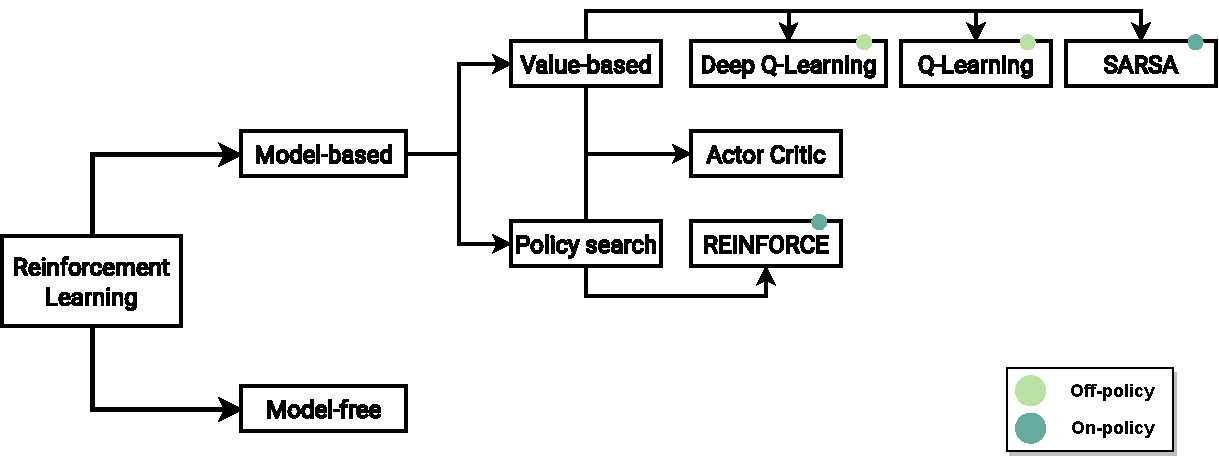
\includegraphics[width=\textwidth]{chapters/img/rl-overview.drawio.pdf}
  \caption{Overview of the \ac{rl} algorithms.}\label{fig:rl:overview}
\end{figure}
In conclusion, 
 this section has provided a comprehensive overview of RL, 
 beginning with the formulation of the problem and the underlying mathematical framework. We also explored various analytical solutions and key algorithms associated with RL. 

Reinforcement learning algorithms can be categorized along multiple dimensions (summarized in \Cref{fig:rl:overview}). 
 One primary distinction is between \emph{model-free} and \emph{model-based} algorithms. 
 In the former, there is no need for a model of the environment, allowing the algorithm to learn directly through interaction. 
 In contrast, model-based algorithms require an MDP to compute the optimal policy.
%
Another important categorization is whether an algorithm is \emph{on-policy} or \emph{off-policy}. 
 On-policy algorithms optimize the same policy that is used for exploration, 
 whereas off-policy algorithms utilize two separate policies during the learning process, commonly referred to as the behaviour and target policies.
%
RL algorithms can be broadly divided based on what they aim to learn. 
 The primary categories here are value-based and policy gradient methods, 
 although hybrid approaches also exist that combine elements of both, like actor critic.
%
Lastly, RL algorithms can be categorized based on whether they use a \emph{tabular} or \emph{approximate} approach. 
 Tabular methods store the value function in a table, 
 while approximate methods leverage function approximation techniques, 
 such as neural networks, to estimate the value function.

This overview serves as a basis for the multi-agent and many-agent RL algorithms,
 because most of the algorithms that we will discuss in the following sections are based on the concepts presented here.

\section{Multi-agent}
\begin{figure}
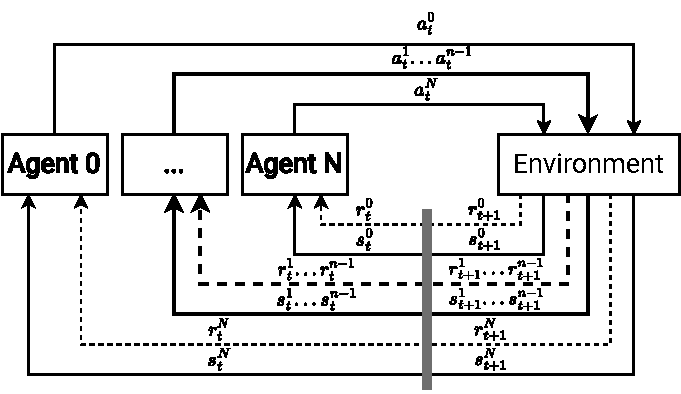
\includegraphics[width=\textwidth]{chapters/img/multi-agent-rl.drawio.pdf}
\caption{Overview of the \ac{marl} framework.}\label{fig:marl:overview}
\end{figure}
In the evolving landscape of \ac{rl}, the concept of \acf{marl} (\Cref{fig:marl:overview}) stands as a natural extension of the foundational \ac{rl} principles. 
 While traditional \ac{rl} generally focuses on the interactions between a single agent and an environment, 
 \ac{marl} broadens the scope to include multiple agents, 
 each with their own objectives, policies, and decision-making processes.

The basic setting in \ac{marl} comprises multiple agents interacting either \emph{cooperatively}, \emph{competitively}, or in a \emph{mixed} fashion within a shared environment---more details in the following sections. 
 Each agent $i$ continues to observe its own state $s_{t}^{i}$, select actions $a_{t}^{i}$ according to its policy $\pi^{i}$, and receive rewards $r_{t+1}^{i}$.
 However, in \ac{marl}, 
 an agent's actions can directly or indirectly influence the states and rewards of other agents, 
 thereby increasing the complexity of the learning problem.
The key challenge in \ac{marl} 
 is to develop robust algorithms that enable agents to learn optimal policies in these complex, often \emph{non-stationary}, environments. 
 Classic \ac{rl} algorithms often require modifications to accommodate the multi-agent setting. 
 For instance, the concept of a joint action space, a state space extended to multiple agents, and a composite reward function are essential considerations.
\subsection{Stochastic games}
The formalization of MARL typically extends the standard Markov Decision Process (MDP) 
 framework to account for multiple agent. 
 One of the most straightforward extensions is the Markov Game, also called Stochastic games. 
 In this formalization, 
each agent has its own state, action, and reward function, 
and the joint actions of all agents determine the transition dynamics and rewards: 
\begin{equation}
S = \langle \mathcal{N}, \mathcal{S}, \mathcal{A}_1, \ldots, \mathcal{A}_N, \mathcal{P}, \mathcal{R}_1, \ldots, \mathcal{R}_N \rangle
\end{equation}
Where:
\begin{itemize}
    \item $\mathcal{N}$ is the number of agents. With $N=1$ we have a single-agent setting, while with $N >> 2$ we have a many-agent setting.
    \item $\mathcal{S}$ is the environment state space. The environment is then considered to be fully observable. 
    \item $\mathcal{A}_i$ is the action space of agent $i$. We denote the joint action space as $\mathbb{A} = \mathcal{A}_1 \times \ldots \times \mathcal{A}_N$.
    \item $\mathcal{P}: \mathcal{S} \times \mathbb{A} \rightarrow \Delta(\mathbb{S})$ is the joint transition probability function. 
    For each time step $t$, $\mathcal{P}$ is a function of the joint action $a_t \in \mathbb{A}$ and the current state $s_t \in \mathcal{S}$, 
    and returns the probability of transitioning to the next state $s_{t+1} \in \mathcal{S}$.
    \item $\mathcal{R}_i: \mathbb{S} \times \mathbb{A} \times \mathbb{S} \rightarrow \mathbb{R}: $ is the reward function for agent $i$. 
    The joint reward function is defined as $\mathbb{R} = \mathcal{R}_1 + \ldots + \mathcal{R}_N$.
\end{itemize}
The game can be described sequentially as follows:
\begin{enumerate}
    \item At each time step $t$, each agent $i$ observes the current state $s_t^i$.
    \item Each agent $i$ selects an action $a_t^i$ according to its policy $\pi^i$.
    \item The joint action $a_t = (a_t^1, \ldots, a_t^N)$ is executed, and the environment transitions to the next state $s_{t+1}$ according to the transition probability function $\mathcal{P}$.
    \item Each agent $i$ receives a reward $r_{t+1}^i$ according to the reward function $\mathcal{R}_i$.
\end{enumerate}
Note that the actions of all agents are executed simultaneously, 
 and each agent's reward depends on the joint action of all agents.
 
\subsection{Taxonomies}
Multi-agent systems can be categorized based on various criteria:

\begin{itemize}
    \item \textbf{Communication}: 
    Agents can either communicate directly with each other or have no communication.
    \item \textbf{Cooperation Level}: 
    Systems can be fully cooperative, fully competitive, or mixed (both cooperative and competitive).
    \item \textbf{Adversarial Nature}:
     Some systems have agents with opposing goals, making them adversarial.
\end{itemize}

\subsection{State-of-the-art}
Recent advancements in MARL have led to the development of algorithms that can handle complex interactions between agents. Some state-of-the-art algorithms include Proximal Policy Optimization (PPO) for multi-agent settings, MADDPG (Multi-Agent Deep Deterministic Policy Gradient), and QMIX.

\section{Many-agent}
The \ac{marl} framework, even if consider multiple agents,
  still assumes that the number of agents is small (i.e. $N \leq 2$).
  For that reason, solutions that work well in \ac{marl} settings may not be suitable for \emph{many-agent} scenarios.

In this thesis, we consider \emph{homogeneous \ac{MAARL}}~\cite{yang2021many}, 
 where the set of agents is large ($N \gg 2$) and each agent is \emph{interchangeable} and \emph{indistinguishable}.
%
This research area is relevant in the context of large-scale systems 
 where collective intelligence emerges from local and repeated interaction of simple entities, like in \ac{cpsw}.
%
In such many-agent scenarios, 
 the implementation of fully decentralized learning is often unfeasible due to the large number of learning agents, 
 which makes the system non-stationary and difficult to manage. 
%
Conversely, a centralized controller capable of coordinating 
 the entire system may not be a viable solution due to scalability concerns. 
 To address this challenge, a practical solution is the adoption of \emph{\ac{CTDE}} approach.
%
The idea is to learn a policy at simulation time when there is a collective view of the system, 
 and then at runtime use that policy but only with local observations. 
%This approach creates policies that are influenced by global information but only require local information to function at runtime. 
%
The typical approach in such cases is based on actor-critic systems~\cite{DBLP:conf/nips/LoweWTHAM17,wu2022more,song2022ctds,song2022centralized},
  where the \emph{actor} is the distributed policy (with only local information) and the critic is a neural network that takes the overall system state.
%
%In fact, the first works in this direction were discussed precisely swarm robotics, %\lukas{what does this mean `in the last field'?}
% exploring new models (e.g., swarMDP~\cite{DBLP:conf/atal/SosicKZK17}) and learning algorithms capable of extrapolating a policy representing the entire system.  \lukas{This sentence still needs rework.}
%Modern approaches, however, 
% have started to consider the use of 
% Recently, deep learning approaches have been considered 
% to synthesise robust controllers capable of generalizing to new tasks. 
%In this context, mean-field reinforcement learning~\cite{pmlr-v80-yang18d} is certainly noteworthy. 
Mean-field RL~\cite{pmlr-v80-yang18d} is one of such concrete applications of \ac{CTDE} 
 where the interactions among the population of agents are estimated by considering either the effect of a single agent and the average impact of the entire population or the influence of neighbouring agents.
%
Some known approaches using mean-field reinforcement learning include Q-mean, 
 which is an extension of Q-learning to mean-field settings~\cite{yang2018mean}, 
 and actor-critic mean-field~\cite{frikha2023actor}, which combines actor-critic algorithms with mean-field approximations. 
%
These approaches have shown promising results in various domains, such as multi-agent coordination 
 and decentralized control, and are actively being researched and developed for further applications.

\subsection{Formalization}
\subsubsection{SwarMDP}
A SwarMDP is characterized by a \emph{swarming agent} ($\mathbb{A}$) and the dynamics of the environment ($\mathbb{E}$).
Specifically, $\mathbb{A}$ is a tuple ($\mathcal{S}, \mathcal{O}, \mathcal{A}, \mathcal{R}, \pi$) where:
\begin{itemize}
  \item $\mathcal{S, O, A}$ are the set of local states, observations (or features), and actions, respectively;
  \item $\mathcal{R}: \mathcal{S} \rightarrow \mathbb{R}$ is the reward function, which is influenced by the environment;
  \item $\pi: \mathcal{O} \rightarrow \mathcal{A}$ is the policy function, which maps the observations to the actions: it could be deterministic or stochastic.
\end{itemize}
Starting from this definition, the environment $\mathbb{E}$ is defined as a tuple ($\mathcal{P}, \mathbb{A}, \mathcal{T}, \xi$), where:
\begin{itemize}
  \item $\mathcal{P}$ is the total number of agents in the systems (the agent population), which is assumed to be fixed;
  \item $\mathbb{A}$ is the defined agent prototype that rules each agent $v \in P$;
  \item $\mathcal{T}: \mathcal{S}^P \times \mathcal{A}^P \times \mathcal{S}^P \rightarrow \mathbb{R}$ is the transition  global function, which is influenced by the actions of the agents and returns a collective reward -- this is typically not known by the swarming agents;
  \item $\xi: \mathcal{S^P} \rightarrow \mathcal{O^P}$ is the global observation model of the systems.
\end{itemize}
\subsubsection{Networked Markov Decision Process}

\subsection{State-of-the-art}
In many-agent systems, the sheer number of agents makes traditional MARL techniques computationally infeasible. Recent advancements focus on scalable algorithms and techniques like mean-field theory to approximate the interactions between agents. Some notable algorithms include Mean Field Q-learning and Graph Neural Networks for many-agent systems.

\section{Gran-challenges}

\printbibliography[title=References,heading=bibintoc]
\end{refsection}

%%%%%%%%%%%%%%%%%%%%%%%%%%%%%%%%%%%%%%%%%%%%%%%%%%%%%%%%%%%%%%%%%%%%%%%%%%%%%%%%%%%%%%%%%%%%%%%%%%%%
%%%%%%%%%%%%%%%%%%%%%%%%%%%%%%% PART II %%%%%%%%%%%%%%%%%%%%%%%%%%%%%%%%%%%%%%%%%%%%%%%%%%%%%%%%%%%%
%%%%%%%%%%%%%%%%%%%%%%%%%%%%%%%%%%%%%%%%%%%%%%%%%%%%%%%%%%%%%%%%%%%%%%%%%%%%%%%%%%%%%%%%%%%%%%%%%%%%

\part{Engineering Cyber-Physical Swarms}\label{part:engineering}
\begin{refsection}
%!TeX root = thesis-main.tex
% revisions
\newcommand{\LP}[2]{\marginpar{$\color{red}\star$}\color{gray}\sout{#1}\color{blue}\
  #2 \color{black}}
\newcommand{\LPr}[2]{{\color{gray}\ #1\ \color{orange}\  #2}}

%\lstset{frame=single,basewidth=0.5em,language={scafi},
%basicstyle=\lst@ifdisplaystyle\small\fi\ttfamily}

%\chapter{A Field-based Computing Approach to Sensing-driven Clustering in Robot Swarms}
\chapter[Sensing-driven Clustering in Swarms]{Sensing-driven Clustering in Swarms: A Field-based computing approach}\label{chap:eng:clustering}\mtcaddchapter
\minitoc% Creating an actual minitoc

\emph{Swarm intelligence}
 is the collective-level ability to solve problems
 in large groups of relatively simple agents that interact with each other locally, i.e., based on physical/logical proximity~\cite{DBLP:books/daglib/0032898}.
%
Common but not exhaustive classes of collective behaviours
 include spatial organization (e.g., pattern formation),
 swarm navigation,
 and collective-decision making~\cite{DBLP:journals/swarm/BrambillaFBD13}.
%

In particular, one problem of interest is \emph{swarm clustering} \cite{DBLP:conf/smc/LeeKK05,DBLP:journals/asc/CruzNM17},
 whereby the classical data clustering task
 (i.e., the unsupervised learning task where data items are grouped to promote intra-group similarity)
 is brought in swarm settings.
%
This problem revolves around splitting the swarm
 into groups of individuals, called \emph{clusters},
 such that the individuals in the same \emph{cluster}
 are more similar to each other (for some definition of \emph{similarity}) than to those in other clusters.
%
Once a cluster is formed, typically it is assigned a \emph{sub-goal} to be carried on collectively.
%
Typical clustering approaches may consider
 the spatial distribution of the individuals
 or the goals of the individuals to define clusters
 \rev{that represent, e.g.,} teams or interaction domains.
%
In this chapter, 
 we focus on \emph{sensing-based clustering}~\cite{DBLP:conf/ccnc/LinM07}, namely
 a clustering problem
 that considers both the spatial distribution of individuals
 and the environmental values sensed by these individuals (through sensors).
 This is essential for \ac{cpsw} applications due to the tight integration with the physical world.
%
That is, the goal is to seek clusters of neighbour individuals with a similar perception of some sensed value.
%
The problem can be in a \emph{static} form,
 where a snapshot of the system state is considered,
 or in a \emph{dynamic} form,
 where values change over time
 and solutions have to deal with change somehow.
%
The problem has been considered in Wireless Sensor Networks (WSNs) and Internet-of-Things (IoT) applications like
  environment monitoring and control~\cite{DBLP:conf/ccnc/LinM07},
  efficient distributed collection~\cite{DBLP:journals/ijcomsys/PhamLPC10},
  and disaster management~\cite{DBLP:journals/jaihc/KucukBSK20}.
%
However, to the best of our knowledge, 
 no existing work addresses the dynamic problem in \ac{cpsw}, which requires specific
techniques to adaptively re-adjust clusters to face changes.
%
Additionally, we look for solutions featuring \emph{resilience}, namely,
 leveraging distribution and decentralization to continuously face changes and faults, hence avoiding single points of failures and potential bottlenecks.
%
%Therefore, i
Accordingly, we present and address the \emph{dynamic sensing-based swarm clustering} problem,
 based on our language-based view of \ac{cpsw}, 
 namely enforcing the use of a field-based programming model, 
 both for the specification of the problem (i.e., the system model) and for the solution (i.e., the distributed aggregate computing program definition).  
%
%In this approach, computations
% leverage an execution model based on repeated computation
% and asynchronous neighbour-based communication.
%
%On top, complex collective behaviour is described in terms of
 %a  functional abstraction, namely, by
% functional manipulations of \emph{(computational) fields}, i.e.,
% data structures evolving over time that map agents in a domain to computational values---sort of % spatially distributed streams of values.
%
%This is inspired by the common notion of fields found in physics (e.g., force or magnetic fields).
%
%Notice, however, that in our viewpoint, the computational fields assign values to agents rather than to environment (space-time) positions as in e.g. \emph{artificial potential fields}~\cite{DBLP:conf/icra/Warren89},
% though the approaches are similar and related.
%
%It has shown to conveniently express
% a variety of \rev{resilient} collective swarm-like behaviour including
% self-healing distance estimation (\emph{gradient})~\cite{DBLP:conf/saso/AudritoCDV17},
% self-stabilising leader election~\cite{DBLP:conf/saso/MoBD18},
 %distributed collection~\cite{audrito2021jcee-distributed-collection},
% and team creation and coordination~\cite{DBLP:journals/eaai/CasadeiVAPD21}---and to scale with complexity up to high-level composite patterns~\cite{DBLP:journals/fgcs/PianiniCVN21}.

Essentially, the core idea of our clustering approach is to make agents
 in local \rev{minima (or maxima)} of the sensed value \rev{(depending on whether lowest or highest values are most significant)} spawn a spatial process of gathering for neighbour devices until finding the proper size of the cluster,
 additionally managing interactions with other clusters when there are overlaps.
%

%\section{Background and Motivation}
\label{s:background}
%\meta{cross-disciplinary approaches $\to$ fields?}

\section{Background: Field-based Concurrent Processes}
\sloppy
Field-based concurrent processes, also called \emph{aggregate processes}~\cite{DBLP:conf/coordination/CasadeiVAPD19,DBLP:journals/eaai/CasadeiVAPD21},
 are field-based computations
 that exist dynamically:
 they can be dynamically generated (usually by individual agents),
 execute on a dynamic set of agents,
 and disappear once all its members withdraw.
%
They have been formalized in \cite{DBLP:conf/coordination/CasadeiVAPD19}
 and deeply covered in \cite{DBLP:journals/eaai/CasadeiVAPD21},
 showing how they can support the design of intelligent collective behaviour by extending the practical expressiveness of field-based programming models~\cite{DBLP:journals/jlap/ViroliBDACP19}.
%
We provide a brief account of the details relevant for this chapter in the following.

Indeed, the aggregate process abstraction
 is relevant since an aggregate process instance,
 by running on a (evolving) subset of the agents,
 can be used to denote a \emph{dynamic} cluster.
%
Therefore, clustering algorithms
 can be expressed in terms of how
 aggregate processes are generated (candidate cluster formation)
 and
 merged/removed (cluster selection).

Aggregate processes can be expressed as normal field-based functions and spawned through a \lstinline|spawn| construct
 with the following signature:
%
\begin{lstlisting}
// spawn is a generic function which accepts 3 parameters
def spawn[K,A,R](process: K => A => (R,Boolean),
                 newProcesses: Set[K],
                 args: A): Map[K,R]
\end{lstlisting}
%
The generic type \lstinline|K| instantiates to the type of \emph{process key}, 
 also called a \emph{process identifier (PID)}, which also works as construction parameter;
 the generic type \lstinline|A| instantiates to the type of runtime parameters for the currently running process instances;
 the generic type \lstinline|R| instantiates to the type of the output of the process.
%
A \emph{process definition} has curried type \lstinline|K => A => (R,Boolean)|, 
namely a function from a value of type \lstinline|K| and a value of type \lstinline|A| to a pair of a value of type \lstinline|R| and a Boolean.
%
The Boolean value, called the \emph{process status}, 
 expresses if the device that has executed a given process instance
 would like to participate in the process (\lstinline|true| status)
 or not (\lstinline|false| status).
%
The crucial point is that every device that participates in a process with PID $\pi$ automatically propagates the process PID $\pi$ to all its neighbours, 
which will run a corresponding process instance when the \lstinline|spawn| function is evaluated.
%
So, the \lstinline|spawn| function accepts a function \lstinline|process| of a field-based behaviour,
 a set \lstinline|newProcesses| of new process instances to be generated locally in the current round,
 and a value of type \lstinline|A| for the runtime input of the instances currently running in the local round of a given device.
%
Notice that, though \lstinline|process| can be a field of functions, 
 it is typically a constant field of the same function, 
 which means that usually a \lstinline|spawn| expression enables running zero or more process instances of the same kind of process.
%
Evaluation of \lstinline|spawn| returns a \lstinline|Map[K,R]|
 (i.e., a hashmap or dictionary) which is a set of entries
 mapping the PIDs of executed process instances (with status \lstinline|true|) to corresponding outputs of type \lstinline|R|.
%

As an example, consider building a separate gradient computation
 for each distinct source agent, that will expand within a certain range $\rho$. 
 This could be coded as follows in ScaFi:
\begin{lstlisting}[mathescape]
type DeviceId = Int
// Process definition as a function
val proc: DeviceId => Boolean => (Double, Boolean) = id => isSource => {
  val output = gradient(id == deviceId())
  val status = if(id == deviceId()) isSource
               else output < $\rho$
  (output, status)
}
// Set of processes to be generated locally
val newProcesses: Set[DeviceId] =
  if(isSource()) Set(deviceId()) else Set.empty
// Expression for handling acquired and generated processes
val gradients: Map[DeviceId,Double] =
  spawn[DeviceId,Boolean,Double](process, newProcesses, isSource())
\end{lstlisting}
%
\rev{In detail, the IDs of sources are used as PIDs; so, for instance, a gradient from agent 7 will become a process with PID 7. The process logic is defined through \lstinline|proc|, which is a function of the PID \lstinline|id| and Boolean argument \lstinline|isSource| denoting whether the running agent is a source, as provided by built-in sensor function \lstinline|isSource()|. In \lstinline|proc|, a gradient is built from the agent whose ID, provided by \lstinline|deviceId()|, matches the \lstinline|id| of the source corresponding to the current process instance. Then, \lstinline|status| is defined \lstinline|true| if the source for the process is still a source or, for non-source agents, if their gradient value is lower than threshold $\rho$. Notice that when the original source is not a source any more, the gradient \lstinline|output| will rise, eventually causing all the agents to leave that process.
%
Value \lstinline|newProcesses| will be a singleton set 
 with the ID of the running device
 when its \lstinline|isSource()| sensor returns true,
 or the empty set otherwise.
%
In the former case, 
 a corresponding process is spawned
 if it did not already exist.
%
The evaluation of the \lstinline|spawn| call, then,
 will run both new and existing processes
 including those executed (and not quit) at the previous round,
  as well as those acquired from neighbours.
%
The output of the \lstinline|spawn| expression
 will be a map from the PIDs of the processes locally executed
 to the value of the gradient (\lstinline|output|) locally computed in those process instances.
}

An example of the dynamics of such a program is provided in \Cref{fig:spawn-dynamics}.
%
In the picture: nodes are agents; labels on nodes are agent IDs; edges denote neighbouring links, over which messages are sent and received; the output of the \lstinline|spawn| expression is shown above the nodes unless it is an empty map (not shown); the different sub-pictures are snapshots of a corresponding hypothetical system state trajectory that may result after multiple rounds of execution in multiple devices.
%
A more thorough introduction and description of aggregate processes together with more examples is available in \cite{DBLP:journals/eaai/CasadeiVAPD21}.

\begin{figure}
\centering
\subfloat[Initial network.\label{fig:spawn-dynamics-a}]{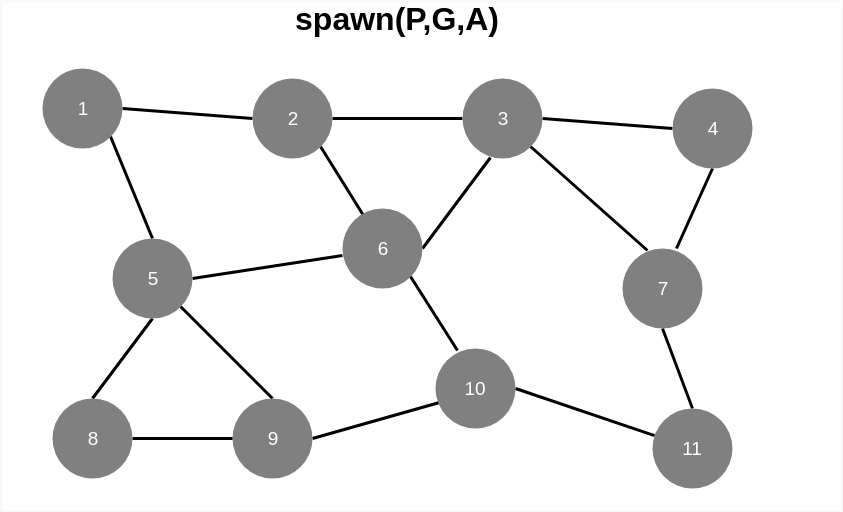
\includegraphics[width=0.45\textwidth]{papers/swarm-intelligence2021/img/spawn-dynamics1.png}}\hfill
%
\subfloat[A process is generated on agent $1$.\label{fig:spawn-dynamics-b}]{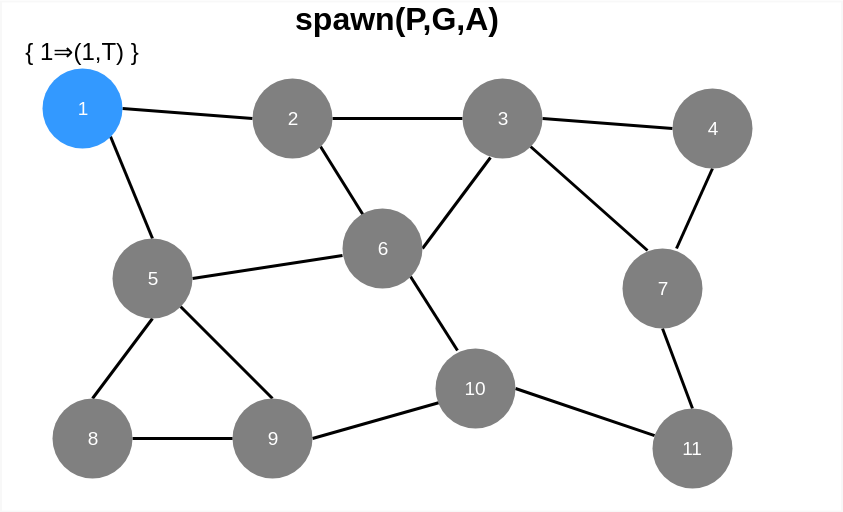
\includegraphics[width=0.45\textwidth]{papers/swarm-intelligence2021/img/spawn-dynamics2.png}}\\
%
\subfloat[The process with PID $1$ propagates up to a certain range.\label{fig:spawn-dynamics-c}]{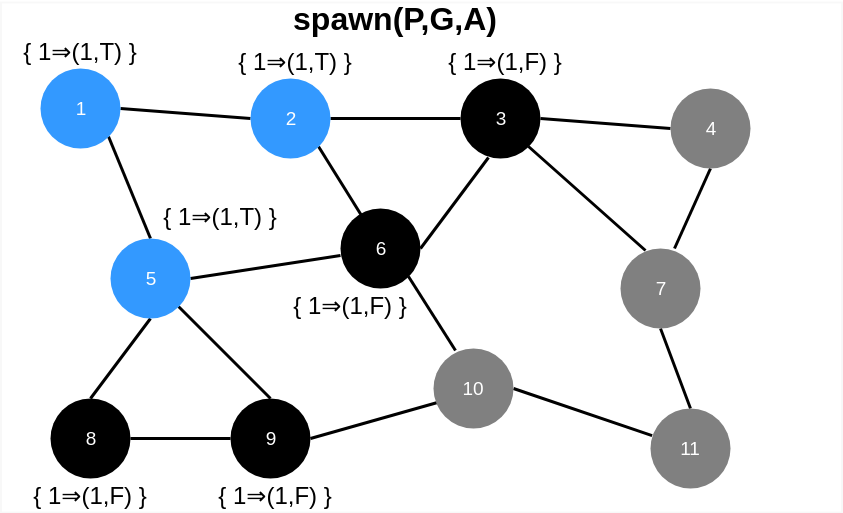
\includegraphics[width=0.45\textwidth]{papers/swarm-intelligence2021/img/spawn-dynamics3.png}}\hfill
%
\subfloat[The ``border'' of a process can change dynamically.\label{fig:spawn-dynamics-d}]{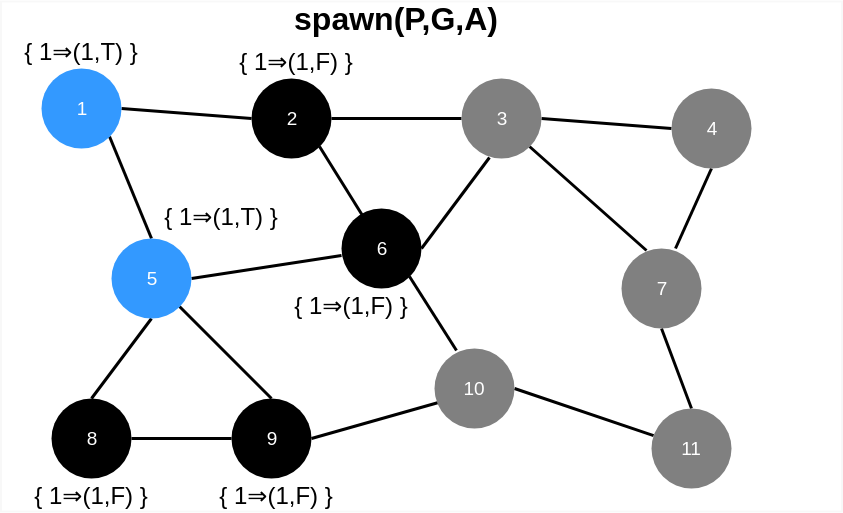
\includegraphics[width=0.45\textwidth]{papers/swarm-intelligence2021/img/spawn-dynamics4.png}}\\
%
\subfloat[Another process is spawned by source agent $3$.\label{fig:spawn-dynamics-e}]{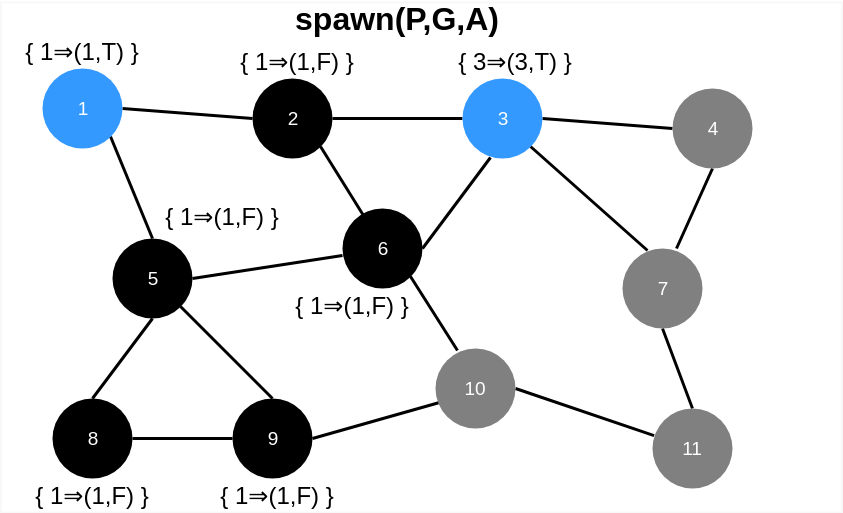
\includegraphics[width=0.45\textwidth]{papers/swarm-intelligence2021/img/spawn-dynamics5.png}}\hfill
%
\subfloat[Processes can overlap. Agents $2$ and $6$ run the two processes with PID $1$ and $3$.\label{fig:spawn-dynamics-f}]{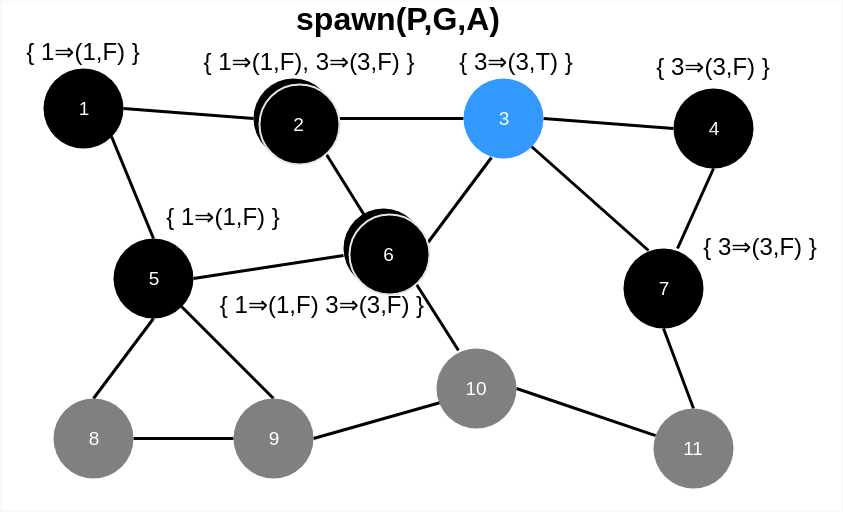
\includegraphics[width=0.45\textwidth]{papers/swarm-intelligence2021/img/spawn-dynamics6.png}}\\
%
\subfloat[Process $1$ ceases to exist.\label{fig:spawn-dynamics-g}]{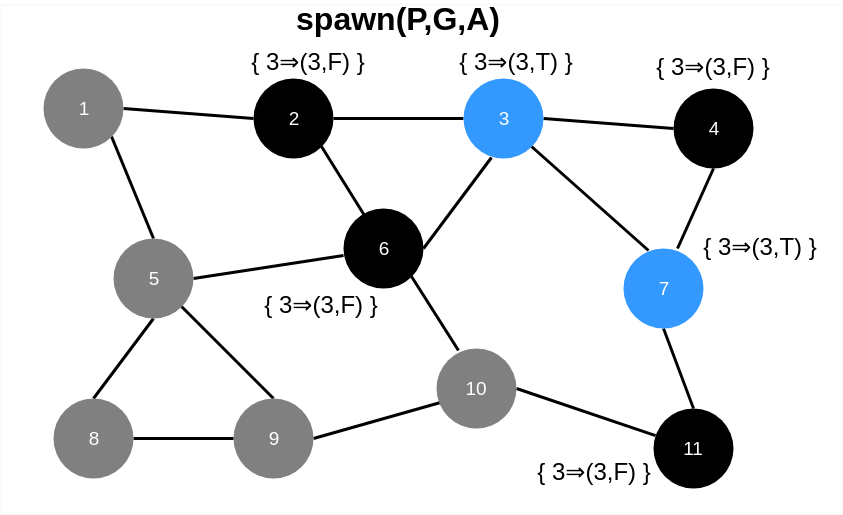
\includegraphics[width=0.45\textwidth]{papers/swarm-intelligence2021/img/spawn-dynamics7.png}}
%
\caption{Examples of the dynamics of multiple concurrent gradient processes.}
\label{fig:spawn-dynamics}
\end{figure}


\section{Resilient Dynamic Cluster Formation}
\label{s:background-clustering}

Different cluster models exist
 and, for each cluster model, several algorithms can be devised~\cite{DBLP:journals/sigkdd/Estivill-Castro02}.
%
These are reviewed and compared with our cluster model in \Cref{s:rw}.

In this chapter, we focus on \emph{swarm clustering},
 which involves associating each swarm member
 to zero or more clusters.
%
So, this is a problem of \emph{cluster formation}~\cite{DBLP:journals/tie/GeHZ18},
 more than a problem of \emph{cluster analysis} (which generally includes cluster formation followed by cluster evaluation).
%
A \emph{cluster}, in this setting,
 is essentially a label (\emph{cluster ID}),
 which can be associated to an agent,
 and that can be used to determine its behaviour.
%
In field terms,
 a clustering can be seen as a field
 mapping each agent to
 a set of cluster IDs---we call this a \emph{clustering field}.

Essentially, a cluster can be used to determine, query, and control a group of agents.
%
Such a group could represent a team, used for cooperation or to solve a common goal,
 or a space-time domain for a field computation.
%
Indeed, as the agents are situated in space,
 they provide a means for extracting data
 from their corresponding location,
 which may be instrumental for environment monitoring,
 data acquisition, etc.

Moreover, we consider \emph{dynamic clustering}~\cite{DBLP:journals/pr/RoaTG19},
 where the emphasis is not on identifying a single clustering
 for a given system configuration,
 but to update and evolve a clustering solution
 as the system configuration evolves
 (e.g., due to mobility, failure, or change in other clustering criteria).
%
The specific problem we tackle is \emph{dynamic sensing-based/space-based swarm clustering},
 which involves associating each swarm member
 to zero or more clusters, and to evolve such association by considering change in the environment (\emph{sensing-based}) and spatial location of the members (\emph{space-based}).
%

In summary, our goal is to define a distributed, decentralized, field-based
 clustering algorithm,
 for the system model based on our language-based view
 described in \Cref{ssec:background:sysmodel},
 able to create and dynamically maintain a clustering field\rev{, resiliently}.
%
\rev{
Our focus on resilience 
 make centralized approaches not appropriate 
 since we cannot assume that some nodes 
 are infallible or always available.
}
%
%This model is different from other clustering models and algorithms as follows.
%%
%\begin{itemize}
%\item Our model differs from \emph{connectivity-based clustering}
% as the topology is already given (neighbourhood-based).
%\end{itemize}
%
This work draws motivation
 from
 (i) the relevance of the problem for \emph{situated} systems as \ac{cpsw},
 (ii) a scarcity of solutions to the problem of \emph{sensing-driven spatial clustering} in literature,
 and
 (iii) a general lack of effective field-based clustering solutions.
%
Refer to \Cref{s:rw} for a more detailed account on these research gaps.


\section{Sensing-Driven Clustering}
\label{s:contrib}

%\meta{ASSIGNED TO: Giorgio (interacting with G. Aguzzi/Ferruccio)}

\rev{
In this section,
 after describing a minimal set of \emph{assumptions}
 underlying the approach (\Cref{ssec:assumptions}),
 we define the \emph{problem} to be addressed (\Cref{ssec:problem-def}), in terms of inputs, outputs, and parameters,
 describe a specific instantiation of the problem for \emph{centroid-based} clustering on numeric values (\Cref{ssec:instantiation}),
 and then present a meta-algorithm providing a solution to the stated problem (\Cref{ssec:meta-algo}).
}


\rev{
\subsection{Assumptions}
\label{ssec:assumptions}
Before formally defining the problem of {\em Dynamic Sensing Based Swarm Clustering}, we summarize the assumptions about the swarm devices and the environment in which they act. Such assumptions justify both the way we define the problem, and some of the design choices we adopt for its solution.
%
\begin{enumerate}
\item A {\em swarm} is composed by a set of possibly many relatively simple autonomous cyber-physical agents, %(e.g., ground, airborne, underwater).
\item An {\em agent} can move within the environment, sense, and actuate.
\item {\em Communication} is based on  peer-to-peer connection link, based on the proximity of agents, without relying on infrastructure (e.g., LTE network, Wi-Fi network).
\item {\em Reliability} of agents themselves and communications are not guaranteed and, in some scenarios, failures are  quite likely.
\item The measures of the {\em environment}, as sensed by the agents, can change over time.
\item The measures of interest of the {\em environment} at two points in space close to each other tend to be positively correlated.
\end{enumerate}
%
The above assumptions, based on our system model defined in \Cref{part:background}, 
 are rather weak and, therefore, quite challenging. 
 They encompass scenarios where a swarm of agents explores an area where multiple natural phenomena are happening. Therefore, even if the proposed solution target \ac{cpsw}, it can be applied to other scenarios, such as WSNs and IoT, where the above assumptions are satisfied.

The field-based clustering algorithm for solving the {\em Dynamic Sensing Based Swarm Clustering} problem will be discussed below. For now, we just want to point out that our assumptions justify a fully distributed approach in which agents exchange information with their neighbours.

First, given the very nature of swarm systems, 
 problems are usually better solved by distributed algorithms than centralized algorithms, e.g., \cite{hoshino:2013,DBLP:journals/asc/CruzNM17}. 
 In particular, by our assumption that agents and communications can fail, 
 and that there is no global communication infrastructure, 
 a node in charge of all the computations (either an agent or a base station) 
 would constitute a risky single point of failure. 
 Even if the swarm was able to recover from such failure by automatically choosing another central node, the switch would be cumbersome and potentially very costly, only to reach again a situation with another single point of failure.

Given agents whose connection links are established and lost based on the proximity with other agents, 
 it may be possible to build an abstraction on top of that, 
 whereby multi-hop communications are transparent, 
 and each agent has the illusion of being able to immediately communicate with any other agent in the swarm by specifying an appropriate ID 
 (this is, e.g., the typical abstraction brought by the IP layer of the TCP/IP stack). 
 While the cost of adding such an additional layer may be acceptable in some situations, for the specific goal of clustering this would not bring any advantage: as we shall see in the sections below, clusters spring out, expand, and collapse following spatial vicinity---i.e., a new cluster expands first to the immediate neighbours of the agent that generated it, and then progressively incrementally spreads to further agents.
}

\subsection{Problem Definition}\label{ssec:problem-def}

We address the problem of situation awareness and recognition, where a value distributed in space (e.g., temperature as measured by sensors) has to be monitored,
 by recognizing compact clusters with similar values (e.g., spatial regions with a similar temperature).
 This problem, called \emph{sensing-driven clustering} in literature, has been investigated largely in static scenarios \cite{DBLP:journals/jaihc/KucukBSK20,DBLP:journals/ijcomsys/PhamLPC10,DBLP:conf/ccnc/LinM07},
 where data from a fixed sensor network has to be processed to obtain the relevant clusters.
 However, solutions for such networks do not extend well to dynamic contexts, such as a mobile \acp{cpsw} system monitoring an environment:
 in this scenario, mobility and proximity of communication are key,
 and need to be handled by an algorithm that is resilient to changes in values, network structure and placement in space.
 To the best of our knowledge, this problem has never been previously considered in the literature.

A sensing-driven clustering algorithm for such system could be useful for several outcomes.
 Clusters may provide a compressed summary of the value distribution in space,
 to upload on the cloud and be graphically represented for human convenience.
%
Clusters may also be used to drive more complex situation recognition patterns:
 algorithms to detect dangerous situations may be run in each cluster separately,
 using information from that cluster to reach a verdict, 
 without interference from information on neighbouring clusters.
 Clusters may also be used to drive task assignments to the monitoring drones,
 possibly guiding their placement in space, by directing more drones in clusters where the need arises.

More formally, we consider the following problem:
\begin{itemize}
	\item \textbf{Input:} for each device, a unique identifier $i$ and a \emph{value} $v_i$ of type $T$ \rev{(possibly obtained through a sensor reading);}
	\item \textbf{Output:} for each device, a list of clusters to which the device belongs, represented as a map from unique identifiers $l$ of cluster leaders to corresponding cluster summary values $w^l$ of type $S$.
\end{itemize}
To formally specify the output, 
 we need some further details characterizing what a \emph{cluster} is, 
 how they should be selected, and what is their \emph{summary}. 
 This is attained through the following problem parameters.
\begin{itemize}
	\item \textbf{Metric:} a data type $M$ with
	\begin{itemize}
		\item a \emph{null} value $0_M$;
		\item a partial order\footnote{A partial order is a reflexive, transitive and anti-symmetric relation; with no requirement that either $x \leq y$ or $y \leq x$ for $x,y$ of type $M$.} $x \leq y$ defined for $x,y$ of type $M$;
		\item an addition operator $x + y$ defined for $x,y$ of type $M$, such that $x + 0_M = x$ and $x + y > x$ if $y > 0_M$;
		\item a positive function $d(i, j) > 0_M$ returning a value in $M$ representing a distance between a device $i$ and $j$ (depending on the devices' sensor states and possibly values $v_i$). \rev{This is intended to make use of spatial distance estimates as well as other factors (i.e., value distances).}
	\end{itemize}
	\item \textbf{Summary:} a data type $S$ with
	\begin{itemize}
		\item a value $s(i)$ of type $S$ in every device $i$ (depending on sensor state);
		\item an associative and commutative function $f : (S,S) \to S$, used to aggregate values $s(i)$ for devices in a same cluster.
	\end{itemize}
	\item \textbf{Leader selection:}
	\begin{itemize}
		\item a candidate radius $r(i)$ in $M$ (depending on sensor state and values), so that only devices with a relative distance strictly lower than $r(i)$ can belong to a cluster whose leader is $i$;\footnote{Notice that $r(i) = 0_M$ implies that no device can be in a cluster whose leader is $i$.}
		\item a commutative similarity predicate $p : (S,S) \to \{\top, \bot\}$, identifying similar clusters based on their summary.
	\end{itemize}
\end{itemize}
According to this description, a candidate cluster $\mathcal{C}$ is a set of devices with a leader $i$,
 such that every $j \in \mathcal{C}$ is within a distance of $r(i)$ from the leader $i$,
 according to the metric given by $d$.
 The summary $w_i$ of such cluster is the repeated aggregation through $f$ of the values $\{v_j : ~ j \in \mathcal{C}\}$.
 Nearby clusters are merged if their summaries are similar according to predicate $p$,
 and in such cases, the lowest identifier is selected as the leader of the merged cluster.

\rev{
Leaders are used to regulating clusters via aggregate processes and to easily support consistent coordination and decision-making regarding the activity of a cluster.
%
Notice that agents 
 may belong to multiple clusters:
 this is important to support 
 tracking phenomena that are spatially close to each other.
%
Indeed, if a node is in between two phenomena,
 it could participate in the corresponding clusters 
 at the same time to help to track
 or handle both phenomena.
}
%
We highlight that we aim to solve this problem by an \emph{adaptive} algorithm,
 that is, a program that is able to handle changes in its input, by periodically and asynchronously updating its internal values.

\subsection{Adaptive Centroid-based Clustering on Numeric Values} \label{ssec:instantiation}

In the evaluation section, we consider a specific instantiation of the \rev{parameters just introduced,}
 for centroid-based clustering on numeric values.
 In this context, the metric is a simple distance on values, so that $d(i, j) = \lvert v_i - v_j \rvert$.
 To prevent the creation of a candidate cluster for every device, 
 the candidate radius $r(i)$ is set to zero whenever $i$ is not a local minimum
 (i.e., has a neighbouring device $j$ such that $v_j < v_i$). 
 If instead $i$ is a local minimum, $r(i)$ is set to a fixed difference value $\theta$.
 The values $s(i)$ to be summarized are set to a tuple $[x_i, y_i, v_i, 1]$ of the devices' positions\footnote{We assume that a GPS-like sensor is available.} and values with the number 1,
 with an aggregator function $f$ that is a component-wise sum, so that the overall aggregate of a cluster $\mathcal{C}$ is (eventually) equal to the tuple
 $[\sum_{i \in \mathcal{C}} x_i, \sum_{i \in \mathcal{C}} y_i, \sum_{i \in \mathcal{C}} v_i, \#\mathcal{C}]$ (where $\#\mathcal{C}$ is the actual number of members of cluster $C$).
 The similarity predicate $p$ then declares two clusters as similar if they have centroids within a radius of $\gamma$,
 in a 3D space mixing spatial coordinates with a value coordinate:
\[
p([x, y, v, n], [x', y', v', n']) \quad\coloneqq\quad \lVert \frac{(x,y,v)}{n} - \frac{(x',y',v')}{n'} \rVert < \gamma
\]
where $(x,y,v)$ denotes a 3D vector and $\lVert \cdot \rVert$ denotes the norm of a vector.
 By setting the problem parameters as described, the meta-algorithm can select clusters of similar value,
 led by their minima, and merge overlapping clusters that are too close together and with a similar value.

\subsection{Adaptive Clustering Meta-Algorithm}
\label{ssec:meta-algo}

We now describe \rev{the general} meta-algorithm for the stated problem through state equations.
 The algorithm state is distributed, hence composed of variables $x_i$ depending on a device identifier $i$:
 we assume that such a variable is stored in device $i$ and periodically updated by it through the state equations.
%
Each equation may involve inspecting the state of variables in neighbour devices $j$:
 we assume that every device periodically shares its state with neighbours,
 so that a (not necessarily updated) view of neighbours' state is available in each device,
 and each state equation can be computed locally in the current device $i$, without remote memory accesses.
%
We use $\mathcal{N}(i)$ to denote the set of current neighbours of device $i$, i.e., the set of devices $j$ for which a view of their state is locally available in $i$ (not including $i$ itself).
 The execution of state equations can be performed in asynchronous rounds, as described in \Cref{part:background}.
 %
 \rev{In order to showcase the algorithm at work by examples, in the following we consider a network of three interconnected devices $i=0,1,2$, so that $\mathcal{N}(0) = \mathcal{N}(1) = \mathcal{N}(2) = \{0,1,2\}$. 
  We assume that the devices are placed in positions $(x_0, y_0) = (0,0)$, $(x_1, y_1) = (1,1)$, $(x_2,y_2) = (2,0)$ and hold values $v_0 = 2$, $v_1 = 3$, $v_2 = 1$. 
  We will also assume that the parameters are as described in Section \ref{ssec:instantiation}, with $\theta = \gamma = 3$.}

\begin{table}
\begin{tabular}{clcl}
$i$ & current device &
$\mathcal{N}(i)$ & neighbour set \\
$\ell$ & candidate leader &
$\mathcal{S}_i$ & candidate leader set \\
$m^\ell_i$ & metric in $i$ from $\ell$ &
$c^\ell_i$ & whether $i$ belongs to cluster $\ell$ \\
$p^\ell_i$ & parent of $i$ in cluster $\ell$ &
$t^\ell_i$ & partial summary in $i$ for cluster $\ell$ \\
$u^\ell_i$ & candidate leader summary in $i$ for $\ell$ \\
$l_i$ & selected leader for cluster $i$, if any &
$w_i$ & selected summary for cluster $i$, if any \\
$l^\ell_i$ & selected leader for cluster $\ell$ in $i$ &
$w^\ell_i$ & selected summary for cluster $\ell$ in $i$
\end{tabular}
\caption{State variables used in the state equations.} \label{tab:variables}
\end{table}

\Cref{tab:variables} summarizes the state variables used in state equations.
 Every device maintains a candidate leader set $\mathcal{S}_i$, of possible clusters to which the device may belong. Every round, this set is updated as:
\[
\mathcal{S}_i ~=~ \{ \ell \in \mathcal{S}_j \text{ for } j \in \mathcal{N}(i) \text{ s.t. } c^\ell_j = \top \} \cup \begin{cases}
	\emptyset & \text{if } r(i) = 0_M \\
	\{ i \} & \text{otherwise}
\end{cases}
\]
Thus, $\mathcal{S}_i$ includes $i$ provided that $r(i) > 0_M$, together with other candidate leaders $\ell$ considered by neighbours
 (in their candidate leader set and which have computed to be within the cluster).
 In field-based computing, this set is implicitly maintained by the \emph{spawn} construct,
 given $c^\ell_i$ as process return status and $\{ i \}$ as new process key (if $r(i) > 0_M$).
 %
\rev{In our sample network, the initial value for $\mathcal{S}_i$ in each $i$ will only consider the current device, as information from neighbouring devices is not available yet. Thus, we will have $\mathcal{S}_0 = \{0\}, \mathcal{S}_1 = \{\}, \mathcal{S}_2 = \{2\}$. After convergence, each node will understand itself as possibly belonging to clusters 0 and 2, so that $\mathcal{S}_0 = \mathcal{S}_1 = \mathcal{S}_2 = \{0,2\}$.}

Most of the meta-algorithm computation is repeated for each of the candidate leaders $\ell \in \mathcal{S}_i$. First, a metric $m^\ell_i$ of the distance between $\ell$ and $i$ is computed,
 through the following equation (i.e., the \lstinline|gradient| block in field-based computing---cf. \Cref{sec:field-calculus-building-blocks}):
\[
m^\ell_i = \begin{cases}
	0_M & \text{if } \ell = i \\
	\min \{m^\ell_j + d(i,j) : ~ j \in \mathcal{N}(i) \} & \text{otherwise}
\end{cases}
\]
\rev{In the sample network, we will have $m^0_0 = m^2_2 = 0$, $m^0_1 = 0 + \vert v_0 - v_1 \vert = 1$, $m^2_1 = 0 + \vert v_2 - v_1 \vert = 2$, $m^2_0 = m^0_2 = 0 + \vert v_0 - v_1 \vert + \vert v_2 - v_1 \vert = 3$. From $m^\ell_i$, we also decide the values $c^\ell_i$ as the truth predicates of whether $m^\ell_i \leq \theta$.}

Then, an optional parent $p^\ell_i$ for $\ell \neq i$ is determined as the neighbour $j$ with minimal $m^\ell_j$ (resolving ties by the identifier $j$ itself):
\[
p^\ell_i = \begin{cases}
	\arg\min_{j \in \mathcal{N}(i)} \{ (m^\ell_j, j) \} & \text{if } \ell \neq i \\
	\text{None} & \text{otherwise}
\end{cases}
\]
\rev{In our example, we have that $p^0_1 = 0$, $p^2_1 = 2$, $p^2_0 = p^0_2 = 1$ while $p^0_0$ and $p^2_2$ are undefined.}
Through it, partial summaries $t^\ell_i$ can be computed (\lstinline|C| block in field-based computing---cf. \Cref{sec:field-calculus-building-blocks}):
\[
t^\ell_i = \text{reduce}(\{s(i)\} \cup \{t^\ell_j :~ j \in \mathcal{N}(i) \text{ and } p^\ell_j = i\}, f)
\]
where ``reduce'' is a function accumulating every element of a given set with the given binary function,
 and thus aggregates with $f$ the value $s(i)$ together with the $t^\ell_j$ values of neighbours $j$ which chose the current device $i$ as their parent.
%
\rev{In the sample network, we will have that $t^2_0 = s(0) = (0,0,2,1)$, $t^0_2 = s(2) = (2,0,1,1)$, $t^0_1 = s(1)+s(2)$, $t^2_1 = s(1)+s(0)$, $t^0_0 = t^2_2 = s(0)+s(1)+s(2) = (3,1,6,3)$.}
%
The value of the partial summary in the leader is then propagated through the cluster by a broadcast function:
\[
u^\ell_i = \begin{cases}
	t^\ell_i & \text{if } \ell = i \\
	u^\ell_{p^\ell_i} & \text{otherwise}
\end{cases}
\]
\rev{so that, in our example after convergence, each $u^\ell_i$ is $(3,1,6,3)$.}
Every candidate leader $i$ with $r(i) > 0_M$ is now able to choose its selected leader $l_i$,
 as the minimum candidate leader $j$ (possibly $i$ itself) with a summary similar to that of $i$ according to predicate $p$:
\[
(l_i, w_i) = \begin{cases}
	\min \{(\ell, u^\ell_i) :~ \ell \in \mathcal{S}_i \text{ and } p(u^\ell_i, u^i_i)\} & \text{if } r(i) > 0_M \\
	\text{None} & \text{otherwise}
\end{cases}
\]
\rev{In the running example, we will have that $l_0 = l_2 = 0$, $w_0 = w_2 = (3,1,6,3)$, since the two clusters are fully overlapping hence $p$ is true.}
The selected leader $l_i$ and corresponding summary $w_i$ is then propagated by broadcast through the cluster of $i$. For every $\ell \in \mathcal{S}_i$:
\[
(l^\ell_i, w^\ell_i) = \begin{cases}
	(l_i, w_i) & \text{if } \ell = i \\
	(l^\ell_{p^\ell_i}, w^\ell_{p^\ell_i}) & \text{otherwise}
\end{cases}
\]
Finally, in every device $i$, the meta-algorithm output is the map:
\[
\{ l^\ell_i \mapsto w^\ell_i :~ \ell \in \mathcal{S}_i \}.
\]

\begin{figure}
\begin{lstlisting}[escapechar=\%, caption=\scafi{} pseudo-code of the clustering meta-algorithm, label={fig:pseudocode}]
// process starts when %$r(i)$% is positive
val newProc = mux (%$r(i)$% > 0) { Set(mid) } { Set.empty }
// collect map from %$\ell \in $% to %$(m^\ell_i, u^\ell_i)$%
val clusters = spawn(%$\ell$% => _ => {
  val %$m^\ell_i$% = gradient(mid == %$\ell$%, %$d$%) // distance estimation
  val %$c^\ell_i$% = %$m^\ell_i$% < %$r(\ell)$% // whether device is in cluster
  val %$t^\ell_i$% = C(%$m^\ell_i$%, %$f$%, %$s(i)$%) // summary collection
  val %$u^\ell_i$% = broadcast(%$m^\ell_i$%, %$t^\ell_i$%) // summary broadcast
  return ((%$m^\ell_i$%, %$u^\ell_i$%), %$c^\ell_i$%) // process result and status
}, newProc, ())
// selected leader
val %$l_i$% = mux (%$r(i)$% > 0) {
  clusters.filter(x => %$p$%(x._2, clusters(mid))).keys.min
} { mid }
// selected leader summary
val %$w_i$% = mux (%$r(i)$% > 0) { clusters(%$l_i$%)._2 } { None }
// propagate in process
val result = spawn(%$\ell$% => _ => {
  val %$m^\ell_i$% = clusters(%$\ell$%)._1 // recover distances
  val %$c^\ell_i$% = %$m^\ell_i$% < %$r(\ell)$% // whether device is in cluster
  val (%$l^\ell_i$%, %$w^\ell_i$%) = broadcast(%$m^\ell_i$%, (%$l_i$%, %$w_i$%)) // final broadcast
  return ((%$l^\ell_i$%, %$w^\ell_i$%), %$c^\ell_i$%) // process result and status
}, newProc, ())
// build result map
return result.map(x => { x._2._1 -> x._2._2 })
\end{lstlisting}
\end{figure}

This meta-algorithm is presented as \scafi{} pseudo-code in \Cref{fig:pseudocode}, using \scafi{} library functions \lstinline|gradient|, \lstinline|C|, and \lstinline|broadcast|---cf. \Cref{sec:field-calculus-building-blocks}.
%
\rev{Notice that since clusters are represented as aggregate processes, and aggregate processes define ``scopes'' for collective computations, the participation of an agent in an aggregate process has by itself the information about the cluster membership; so, collective tasks may be assigned to any cluster, and these will be inherently played by all the members of that cluster.
}
%
 We also remark that although values $v_i$ are not directly used by the meta-algorithms, the parameters $r(i)$ and $d(i,j)$ are allowed to depend on them (and usually do),
 so that values are indirectly used. An example of such behaviour is given in the next section.

%figura della composizione blocchi?
%vedi anche: https://github.com/metaphori/paper-2021-swarm-intelligence-si/blob/master/_Brainstorming/algorithm2.md

\section{Evaluation}
\label{s:eval}

%\meta{ASSIGNED TO: G. Aguzzi / Roby}

In this section, we evaluate the meta-algorithm proposed in \Cref{ssec:meta-algo}
 in a case study of situation recognition within a synthetic environment \rev{(\Cref{s:scenario-description})}.
%
The goal \rev{(\Cref{s:eval-goal})} is to show how the algorithm
 can cluster agents in a sensing-based fashion,
 hence identifying various temperature cluster shapes.
%
Furthermore, we assess how the algorithm works in mobile settings,
 where a swarm of agents moves across an environment---which can be representative for exploration scenarios.
%
\rev{After describing the scenario and goals,
 in this section we describe the simulation framework (\Cref{s:eval:sim-framework}), 
 the simulation configurations (\Cref{s:simulations}),
 the results (\Cref{s:eval:results}),
 and finally provide a discussion about the evaluation and the approach (\Cref{sec:eval-discussion}).
}

%would exemplify the need for the algorithm macro-steps to find good clusters and the algorithm reaction to mobility.

\subsection{Scenario Description}\label{s:scenario-description}
%
A swarm group of \emph{robots} is interested in identifying areas
 where environmental data varies within a known range.
%
In particular, we assume that the robots are both
 capable of sensing the environmental temperature,
 perceiving their position in space (e.g., using GPS),
 and exploring a limited area (i.e., a square with a side of \SI{1}{\kilo\metre}).
%
The temperature is just an arbitrary choice of
 a sensible physical quantity
 that should drive, together with the spatial distribution,
 the clustering;
 the idea is that a temperature can be indicative for
 an environment situation that could require attention or intervention (cf. wildfires which can start and spread in hot, dry, and windy conditions).
%
The scenarios are plausible, but we are not interested in full realism: simplifications and generalizations are introduced to study the algorithm in diverse controlled situations.
%
Since the absence of central authority and the limited agent communication capability,
 we suppose that the agents can only interact with their neighbours
 (i.e., the devices with which a agent manages to establish a connection).
In particular, we imagine that each agent is equipped with a LoRa module with
 a connection range of \SI{100}{\metre}.
%
\rev{
In this case, a node can potentially participate in several clusters
 as it may be spatially close to two different phenomena.
 Therefore, it must both partake in the collective perception
 (i.e. perceive the local temperature)
 and act to solve the cluster-identified problem.
The choice of how and when a node should
 act depends on the application but is typically
 left to the leader,
 since it has the cluster-side vision of phenomena and the nodes.}
%
Notice that these assumptions are coherent with the system model of \Cref{ssec:background:sysmodel}.

In the experiments described in the following,
 we are only interested in the clusters determined by the swarm cooperatively,
 not in \emph{how} clusters are leveraged at the application level.
\rev{
However, even if we do not directly leverage the output of the clustering process,
 we would highlight that, in using the proposed algorithm,
 we inherently exploit \emph{both} the leader election process and the multi-cluster formation.
The foster is necessary to create clusters since,
 in our algorithm, each cluster is managed by \emph{one} leader.
 The latter is essential to track the phenomena of interest.
In fact, as phenomena can be spatially close and thus overlapping,
 if a node could only participate in one cluster,
 we would not be able to analyse the traced phenomenon correctly.}
%
%We intend to evaluate this aspect in future works.
Lastly, we emphasize that the scope of this application is quite versatile and can be adapted to various specific scenarios as outlined in previous research~\cite{DBLP:journals/firai/SchranzUSE20}. 
 Examples include marine monitoring~\cite{Farinelli2017-ic} 
 (covering aspects like aquaculture, pollution, and water quality), 
 intelligent agriculture~\cite{DBLP:conf/fsr/BallREPUFSWC13} (involving fertilization and pest control), 
 military surveillance, tracking of criminal activity, and 
 locating victims in disaster situations~\cite{Saez-Pons2010-hh}.
\subsection{Evaluation Goals}\label{s:eval-goal}
We set up these simulations to:
\begin{enumerate}%[label=\textbf{G.\arabic*}]
\item \label{goal:1} verify the capability of the algorithm to find different cluster shapes: To assess the algorithm's versatility, we aim to confirm its robustness in accurately identifying various types of data distributions, including but not limited to Gaussian shapes;
\item \label{goal:2} examine how \rev{found clusters} can cope with drone movement \rev{and failures}:
  upon confirming the algorithm's effectiveness in stationary conditions, we intend to explore its responsiveness to variables such as drone \emph{mobility} and system \emph{failures}. 
  Our analysis will focus on how these dynamics affect the clustering process in terms of cluster count, shape, and size;
 \item \label{goal:3} test the algorithm dynamics when the temperature distribution changes:
 \rev{
  in a swarm agentics context, the observed phenomena could change over time.
  Therefore, the algorithm proposed should be robust against phenomena dynamisms.}
\end{enumerate}
%
That is, these goals reflect
 the design requirement of
 supporting
 sensing/spatial-based clustering
 in static, mobile, and environment-dynamic scenarios.

\subsection{Simulation Framework}\label{s:eval:sim-framework}

We verify our sensing-driven clustering algorithm using Alchemist simulations.
The simulation experiments, resulting data, source code, and instructions for reproducibility are available at a public GitHub repository\footnote{\url{https://github.com/cric96/experiment-2021-swarm-intelligence-si}}.
%
Alchemist is already used in similar scenarios~\cite{DBLP:journals/eaai/CasadeiVAPD21}, and it supports the \scafi{} language~\cite{DBLP:conf/isola/CasadeiVAD20},
 that has been chosen among other field-based languages~\cite{DBLP:journals/jlap/ViroliBDACP19} as it supports aggregate processes~\cite{DBLP:conf/coordination/CasadeiVAPD19},
 which we consider essential in order to implement our clustering algorithm.

\subsubsection{Parameters}

To evaluate the efficacy of our proposed solution, we examine the collective program behavior under various parameters. 
 These parameters are summarized in \Cref{table:parameters} and elaborated upon below.

A key parameter is the \emph{in-cluster threshold} ($\theta$), 
 which serves as a determinant for whether an agent resides within or outside a cluster. 
 This threshold plays a critical role in guiding the expansion of the aggregate process across nodes. 
 A low value may limit the program's consideration to only a handful of nodes, 
 whereas an excessively high value could result in the inclusion of nodes that should not be part of the cluster. 
 Given that this parameter is contingent on the specific application, 
 developers need to judiciously strike a balance between node inclusion and boundedness, 
 as this will significantly influence the shape of the cluster.

The \emph{same cluster threshold} ($\gamma$) is employed by the cluster leader to determine the similarity between two clusters, 
 as elaborated in \Cref{ssec:meta-algo}.
%
This parameter is vital in accurately establishing cluster boundaries. 
 A high value for $\gamma$ could result in the merging of two distinct clusters, 
 while a value that's too low might leave overlapping clusters separated even when they could be meaningfully combined.

A clustering process starts when a node becomes a candidate.
 \emph{waiting candidate time} ($\beta$) rules the rounds needed by a node to spawn a process after it has become a candidate.
 This helps in avoiding the excessive process spawn due to small local temperature variations.

We are interested in the robustness of the clustering process against the robots movement. Therefore, we tested our
 solution varying the robot \emph{speed} ($\omega$) and the \emph{exploration range} ($\zeta$).
 We expect that the higher the movement speed, the greater the instability of the identified clusters.
 $\omega$ does not affect candidate robots, they will stand still until they stay candidates.

We check also how the output changes varying the \emph{density} ($\alpha$) of robots.
 Theoretically, we expect a better result with high-density swarms.
 \rev{From $\alpha$ we compute the total number of robots as:}
$
 N = (10 / \alpha) ^ 2
$,
e.g. with $\alpha = 0.5, N = 400$ and with $\alpha = 0.75, N = 173$.

\rev{
Finally, $\xi$ (\emph{failure frequency}) and $\tau$ (\emph{spawn frequency})
 are used to verify how our algorithm
 could handle failures during the clustering process.
 The foster rules the frequency in which
 a random node disappears from the system.
The latter controls the rate of spawning nodes
 that will participate in the aggregate program evaluation.
This is useful to avoid complete node isolation after frequent node failures.
 Even if the movement is already a good estimation of how the system responds
 to dynamisms, we want to add another disruptive change.
Indeed, movements are typically relative,
 and therefore the changes in the neighbourhood are limited.
}
\begin{table}[t]
  \centering
  \resizebox{\textwidth}{!}{
    \begin{tabular}{|p{0.30\linewidth}|p{0.05\linewidth}|p{0.35\linewidth}|p{0.15\linewidth}|}
      \hline
      Parameter                          & Unit & Description                                                                                                                     & Values                \\ \hline
      In Cluster Threshold   -- $\theta$ & \unit{\celsius}                                  & A real value used to verify if the temperature perceived in a certain node could be considered as a part of the current cluster & {[} 0.5, 1.0, 1.5 {]} \\ \hline
      Same Cluster Threshold -- $\gamma$ &  n.a                                             & A real value used to verify if two clusters could be considered as the same                                                     & {[} 0.1, 0.3, 0.7 {]} \\ \hline
      Speed                  -- $\omega$ & \unit[per-mode = symbol]{\kilo\metre\per\second} & The constant velocity used by drone to explore the areas                                                                        & {[} 7, 10, 14 {]}     \\ \hline
      Exploration range      -- $\zeta$  & \unit{\kilo\meter}                               & The maximum range area in which drones could move                                                                               & {[} 0.5, 0.6 {]}      \\ \hline
      Density                -- $\alpha$ &  n.a                                             & A parameter used to define how many nodes will be placed in the environment                                                     & {[} 0.5, 0.75 {]}     \\ \hline
      Waiting candidate time -- $\beta$  &  n.a                                             & Rounds needed to mark a node as candidate                                                                                       & {[} 3, 5, 7 {]}       \\ \hline
      Failure frequency      -- $\xi$    &  \unit{\hertz}                                   & Failure frequency of random nodes that participate in the system                                                                                       & {[} 0.5, 0.1, 0 {]}    \\ \hline
      Spawn frequency        -- $\tau$   &  \unit{\hertz}                                   & Spawn frequency of a node in a random position within the environment                                                                           & {[} 0.5, 0.1, 0 {]}    \\ \hline
    \end{tabular}
  }
  \caption{A summary of the parameters used in simulations}
  \label{table:parameters}
\end{table}

\subsubsection{Metrics}

The clustering results are verified using different metrics. First,
 we extract the number of total unique clusters found by the collective
 to check if the program produces the correct partitioning.
%
This value gives a quick overview of the clustering result. 
Along with this value, we
 evaluate the total number of unique merged clusters.
 The latter should be as near as possible to the correct cluster number.

However, neither the number of total unique clusters nor the total number of unique merged clusters
 tells us anything about the shape of the clusters.
 To this aim, we compute several metrics:
 \begin{itemize}
   \item the number of nodes for each cluster, stating the overall device partitions;
   \item the Silhouette~\cite{ROUSSEEUW198753} and Dunn~\cite{dunn1974well} indexes, used as internal
    evaluation schemes;
  \item the error rate, observable only when we know the ground truth.
 \end{itemize}
By examining the Silhouette index, we can gauge the extent to which the clusters overlap. 
 A Silhouette value approaching 0 indicates overlapping clusters, 
 while a value closer to 1 suggests that the clusters are distinct and well-separated. 
 The Dunn index serves as a supplementary metric; 
 when the Silhouette index is close to 1, a higher Dunn index value is expected.
%
The error rate metric quantifies the degree of node misclassification. 
 A node is considered misclassified if it is either falsely associated with a cluster 
 (false positive), or if it is incorrectly identified as external when it should actually belong to a cluster (false negative). 
 The error rate is calculated using the following formula:
 \[
   E = \frac{FP + FN}{TP + TN}
 \]
Here, 
 \( TP \) denotes \emph{true positives}, 
 which refers to the number of nodes correctly classified within a cluster and located near a specific variable like temperature distribution. 
 \( TN \) represents \emph{true negatives}, 
 or the number of nodes accurately classified as external and distanced from any variable distribution. 
 This metric provides insights into the algorithm's performance during drone exploration. 

\subsection{Simulations}\label{s:simulations}
\begin{figure}[t]
  \centering
  \begin{subfigure}[b]{0.2\textwidth}
      \centering
      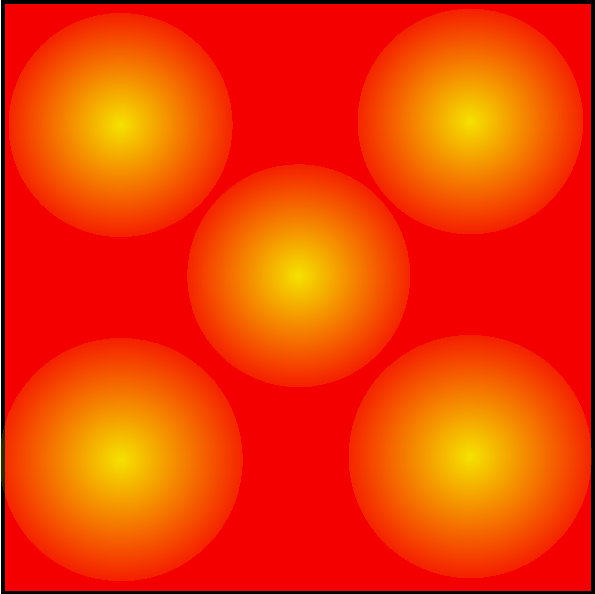
\includegraphics[width=\textwidth]{papers/swarm-intelligence2021/img/scenario/standard}
      \caption{}
      \label{fig:standard}
  \end{subfigure}
  \hfill
  \begin{subfigure}[b]{0.2\textwidth}
      \centering
      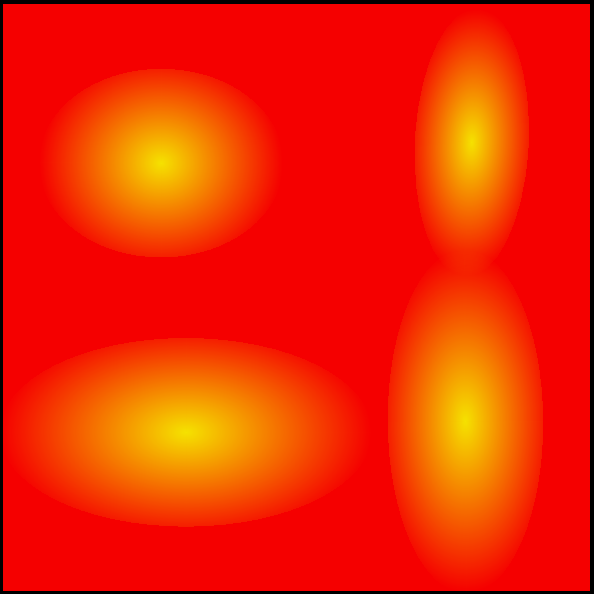
\includegraphics[width=\textwidth]{papers/swarm-intelligence2021/img/scenario/stretched}
      \caption{}
      \label{fig:stretched}
  \end{subfigure}
  \hfill
  \begin{subfigure}[b]{0.2\textwidth}
      \centering
      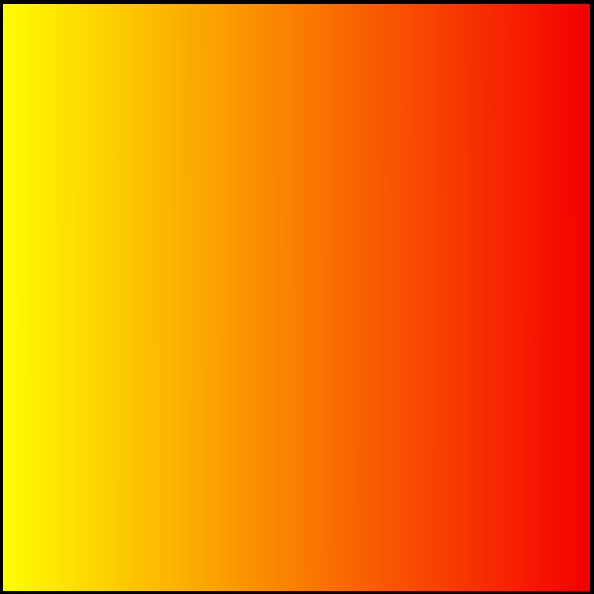
\includegraphics[width=\textwidth]{papers/swarm-intelligence2021/img/scenario/one-direction.pdf}
      \caption{}
      \label{fig:one-direction}
  \end{subfigure}
  \\
  \centering
  \begin{subfigure}[b]{0.2\textwidth}
      \centering
      
\includegraphics[width=\textwidth]{papers/swarm-intelligence2021/img/scenario/one-direction-one-candidate.pdf}
      \caption{}
      \label{fig:one-direction-one-candidate}
  \end{subfigure}
  \hfill
  \begin{subfigure}[b]{0.2\textwidth}
      \centering
      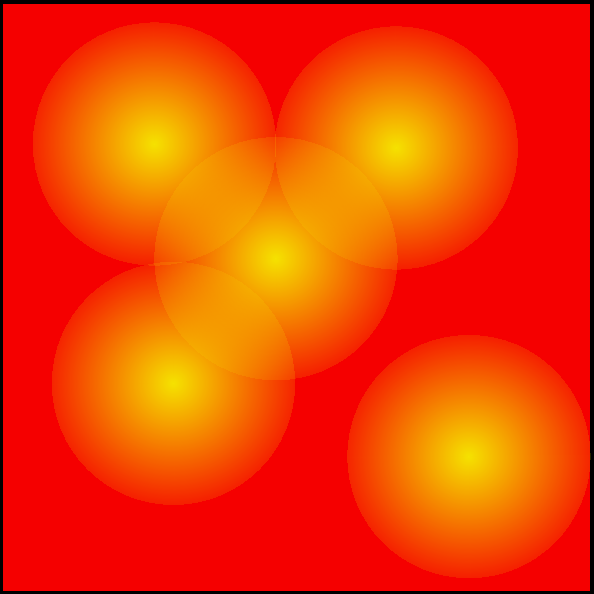
\includegraphics[width=\textwidth]{papers/swarm-intelligence2021/img/scenario/standard-overlay.pdf}
      \caption{}
      \label{fig:overlapped}
  \end{subfigure}
  \hfill
  \begin{subfigure}[b]{0.2\textwidth}
      \centering
      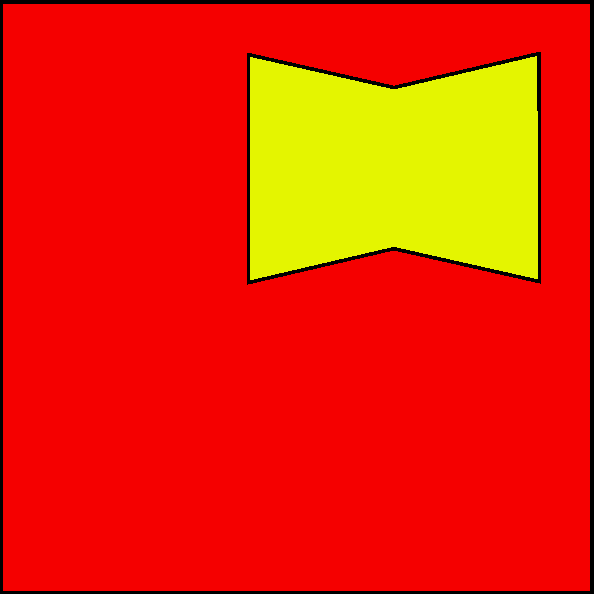
\includegraphics[width=\textwidth]{papers/swarm-intelligence2021/img/scenario/non-convex.pdf}
      \caption{}
      \label{fig:non-convex}
  \end{subfigure}
  \caption{Graphical representation of temperature field distributions used in the simulations. 
  The lighter the colour, the lower the temperature. }
  \label{fig:field-phenomena-distribution}
\end{figure}
\begin{figure}[t]
  \begin{subfigure}[b]{0.45\textwidth}
    \centering
    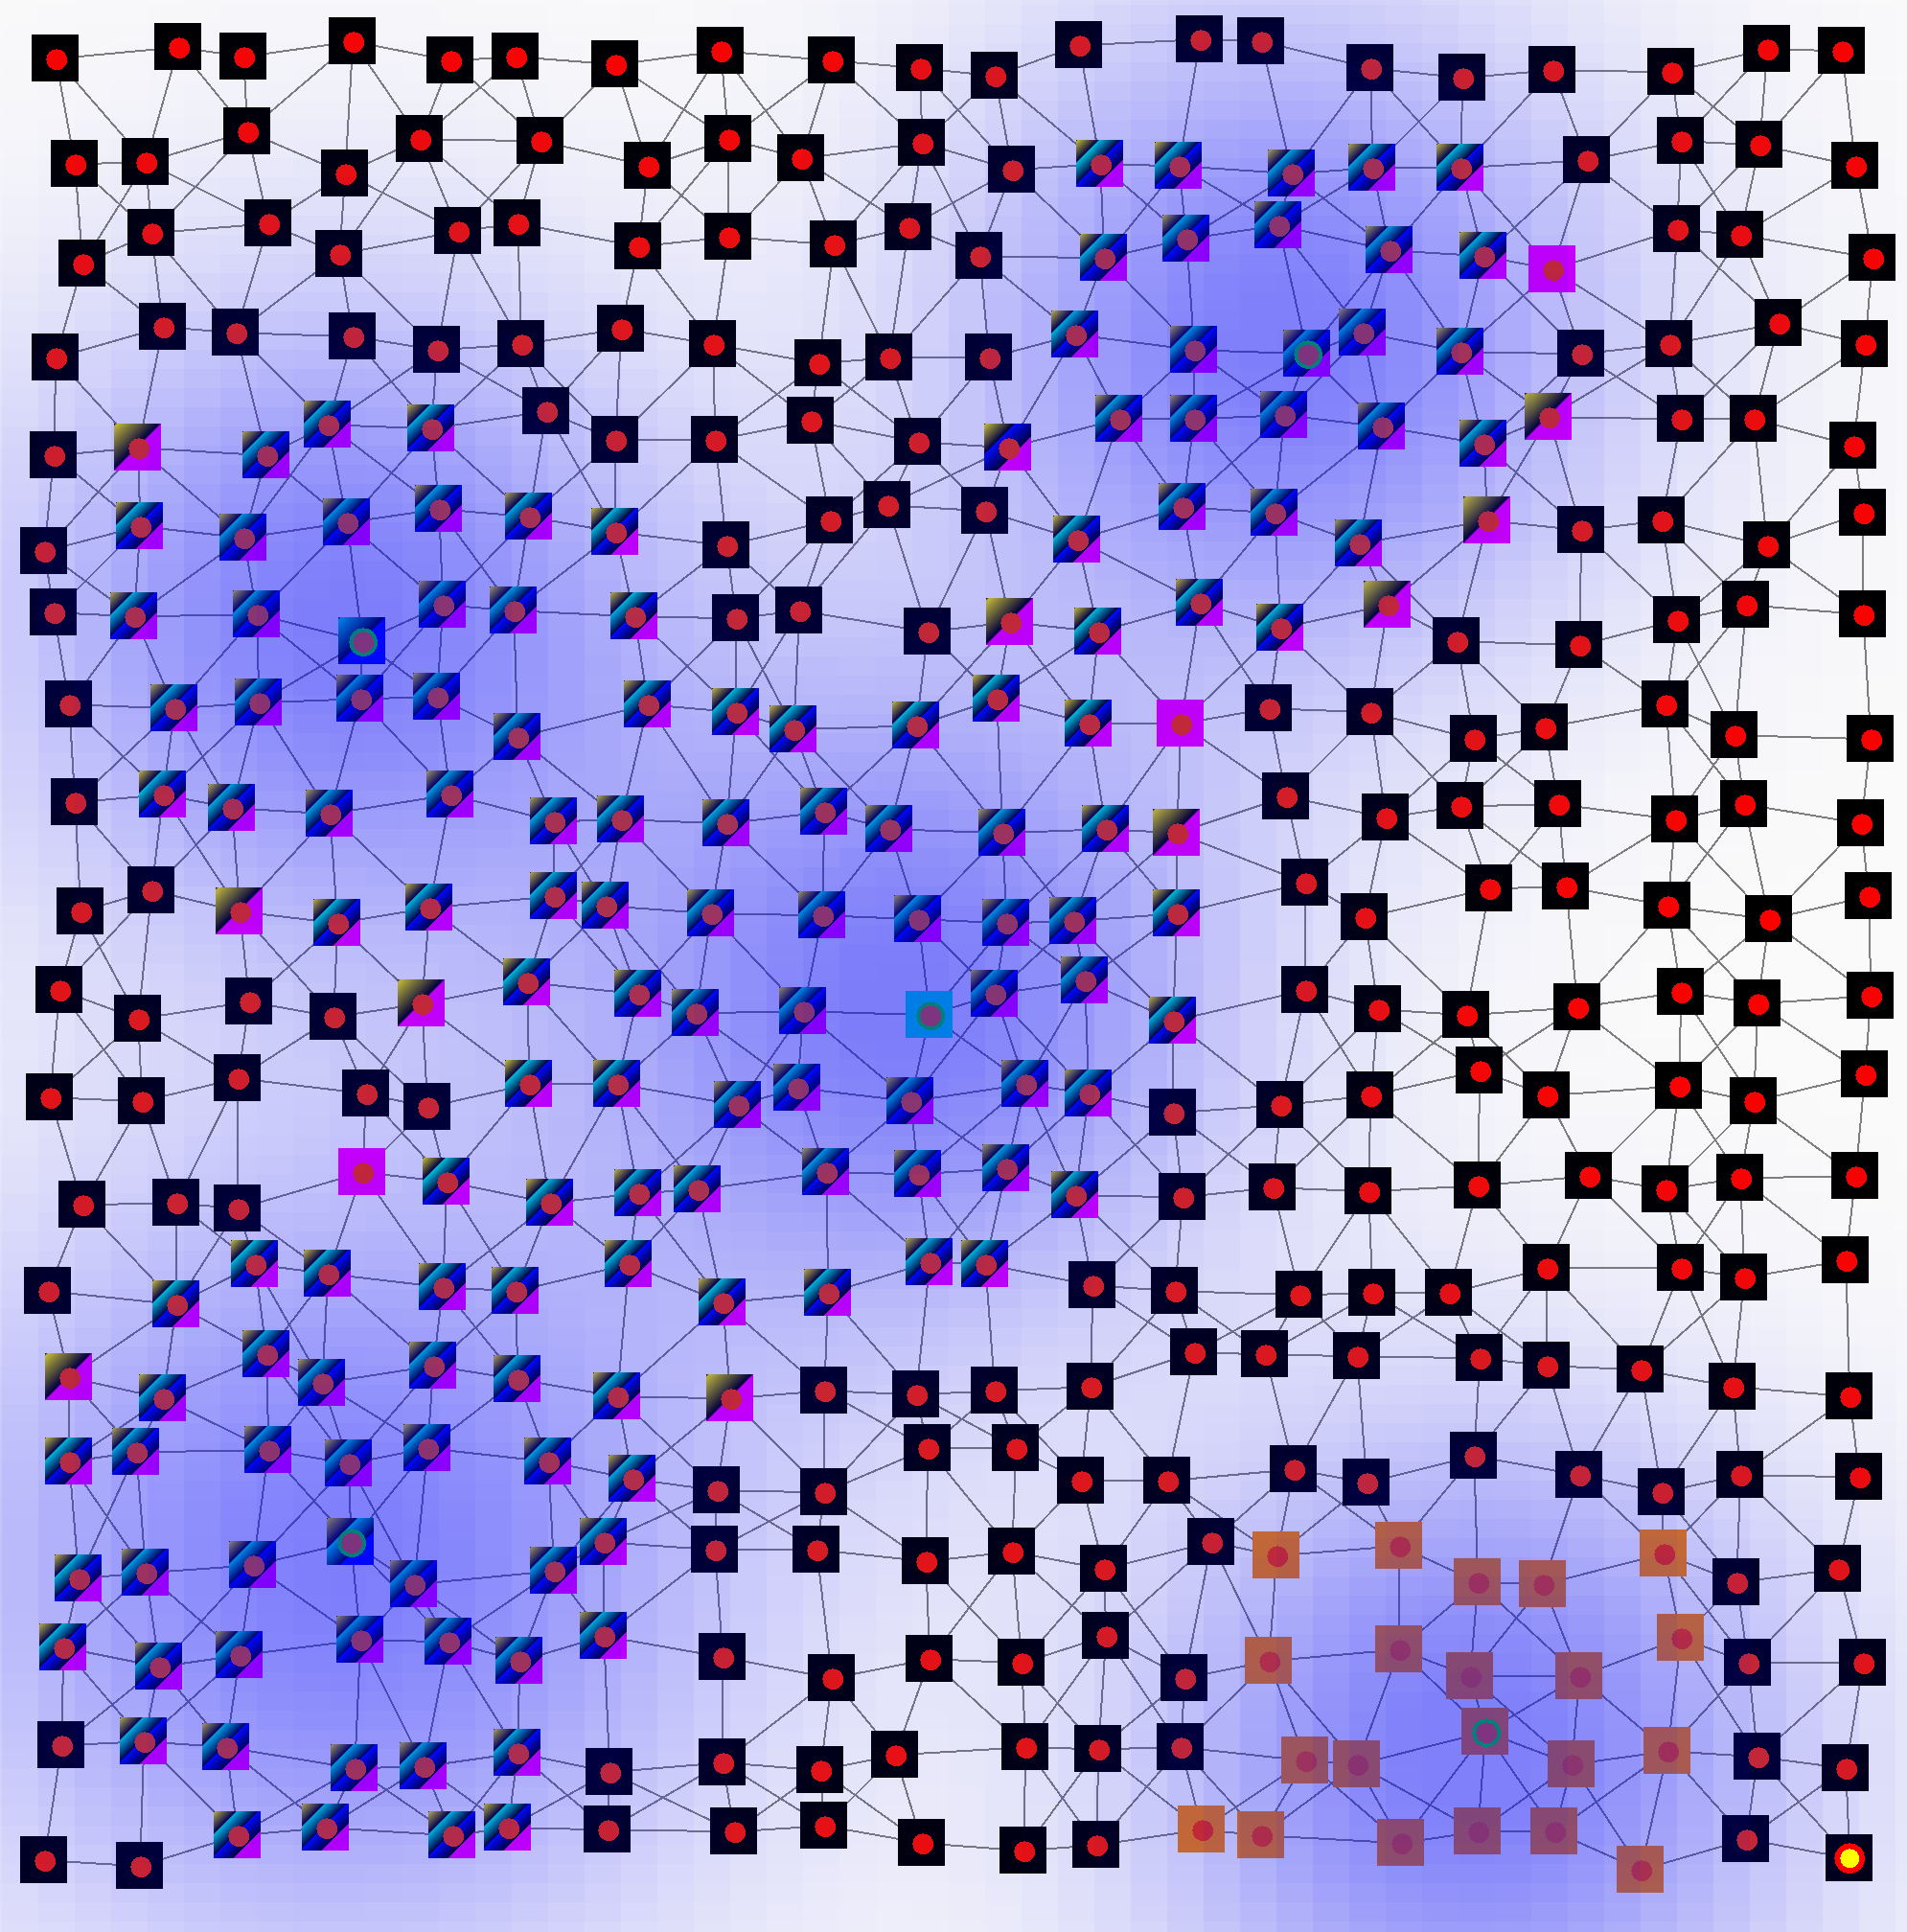
\includegraphics[width=\textwidth]{papers/swarm-intelligence2021/img/simulation-execution.png}
  \end{subfigure}
  \begin{subfigure}[b]{0.45\textwidth}
    \centering
    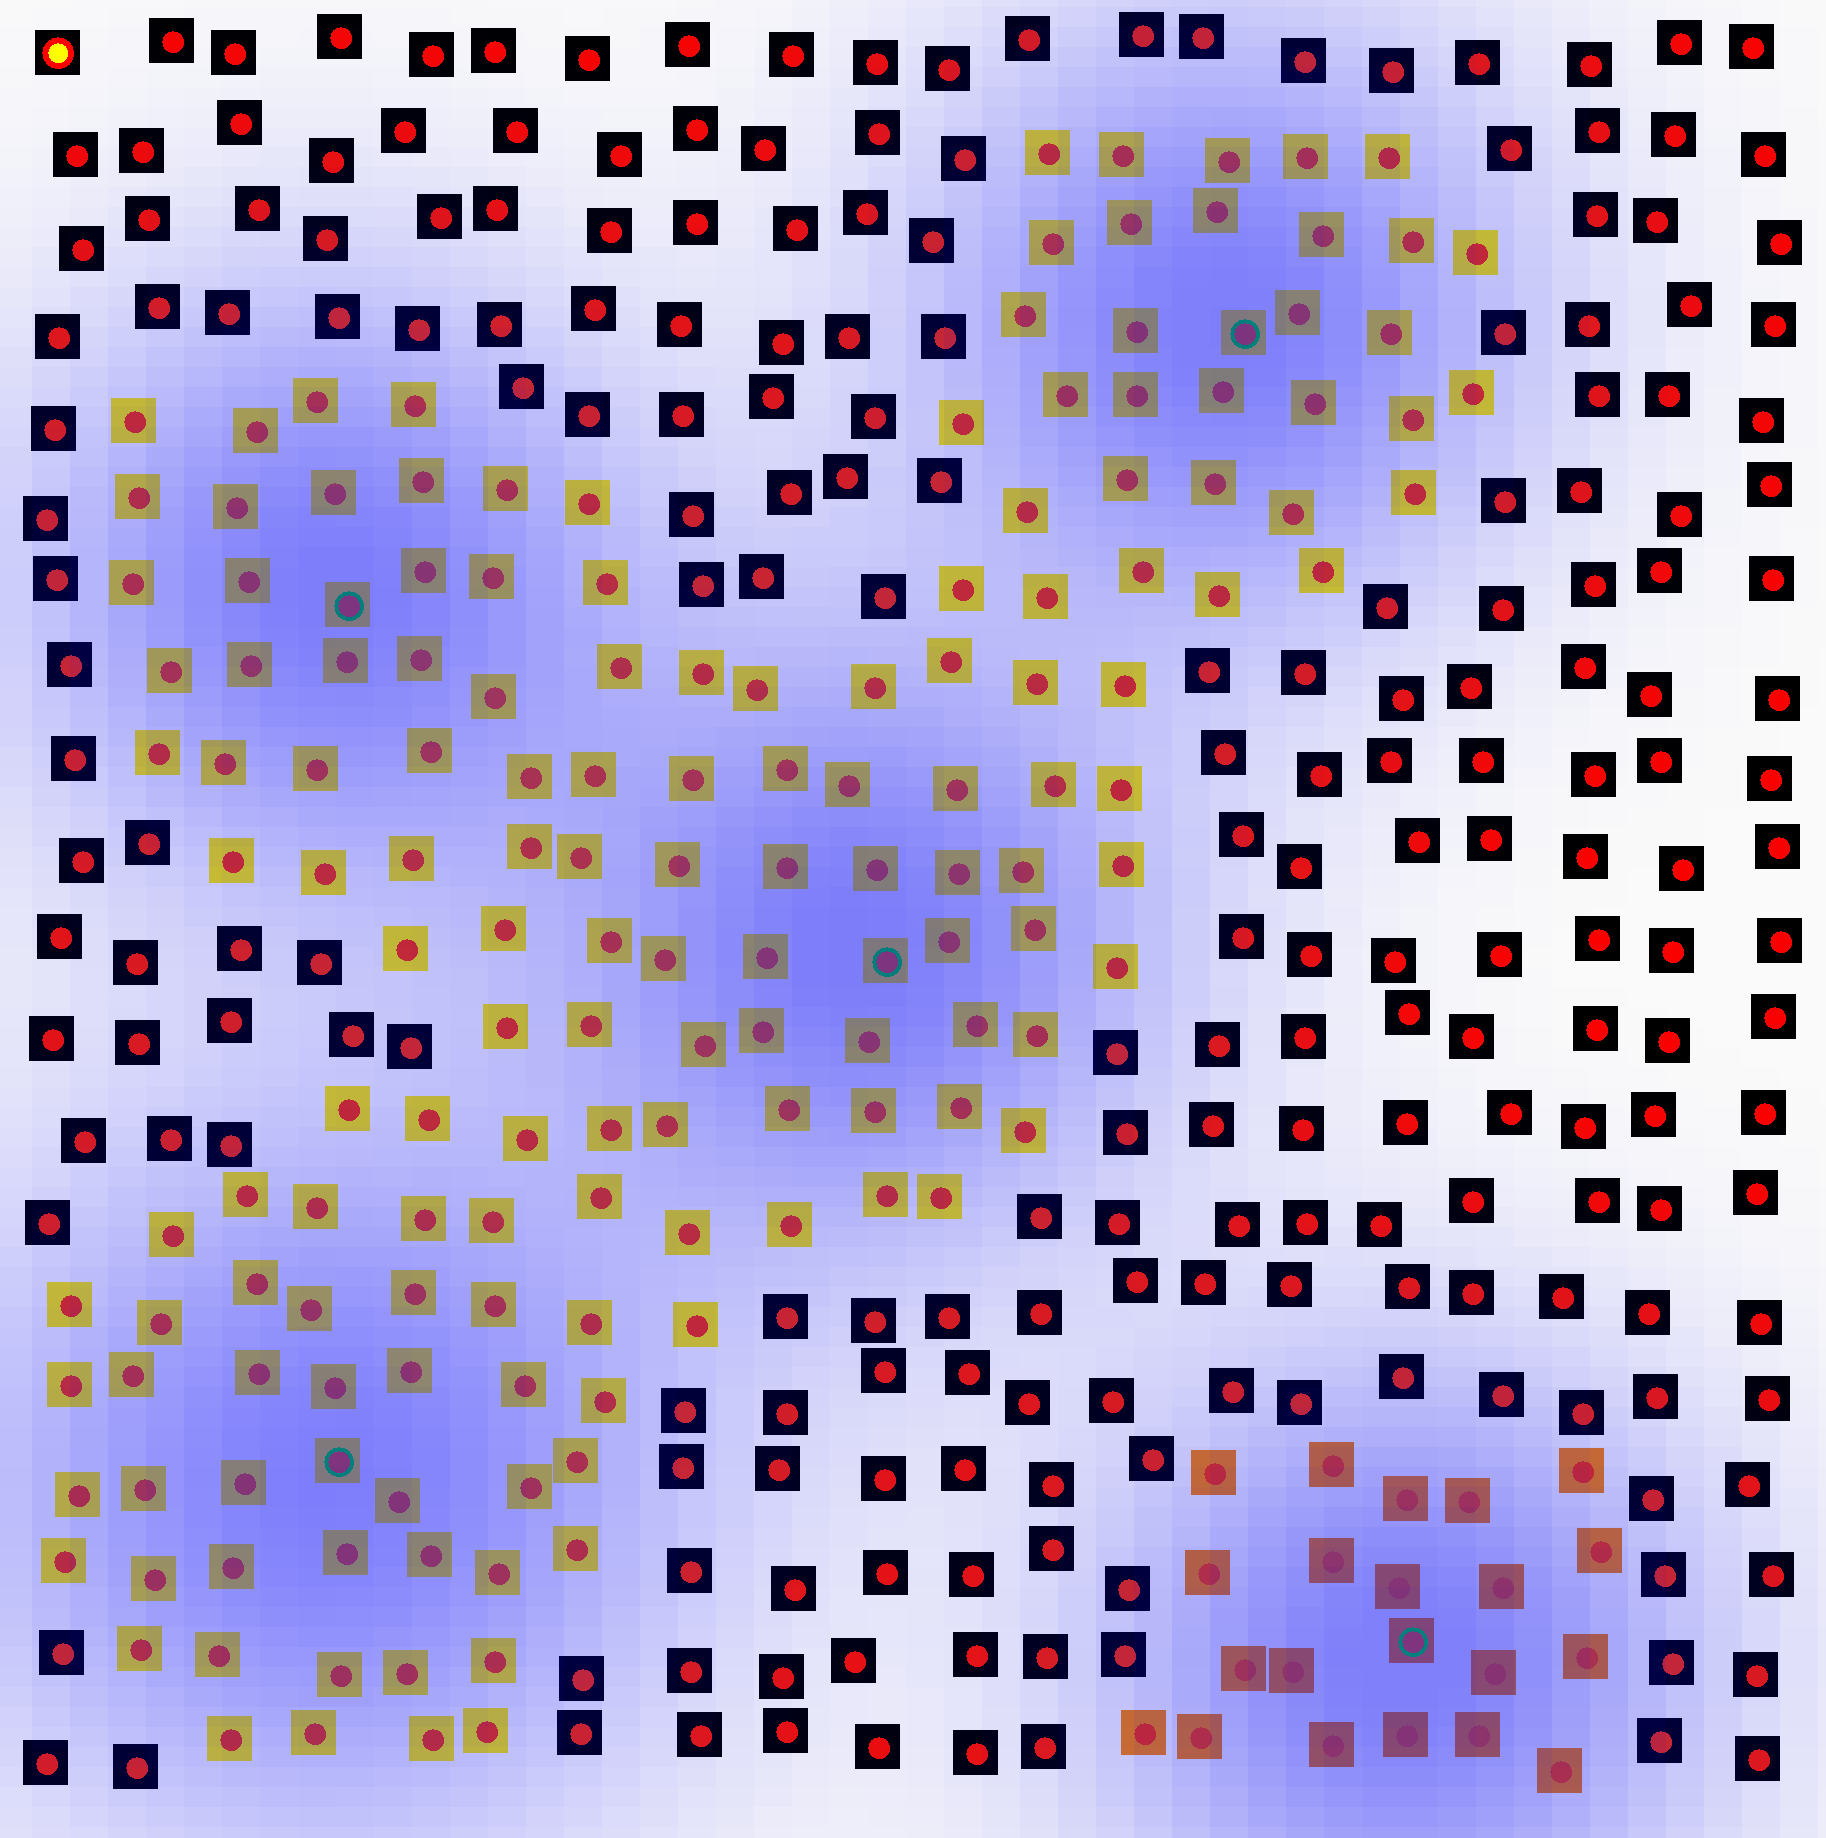
\includegraphics[width=\textwidth]{papers/swarm-intelligence2021/img/after-merge.png}
  \end{subfigure}
  \centering
  \caption[Snapshots of simulation executions during the sensing-driven clustering.]{Snapshots of simulation executions. 
  The colour of the square identifies the cluster ID found in that point. 
  Black colour means no cluster. 
  The green circle means that the node is a candidate. 
  The blue gradient circles are a graphical representation of temperature distribution. 
  On the left is shown a snapshot of a simulation before the merge policy has been applied (multiple clusters per point are found). 
  On the right, there is the snapshot of the same simulation after the merge policy action.}
  \label{fig:simulation-snapshot}
\end{figure}

We evaluate the behaviour of our algorithm in several experiments. %(explained below and illustrated in \Cref{fig:field-phenomena-distribution}).
 The simulations have in common
 \begin{enumerate*}%[i)]
  \item the environment area (a square with a side of 1km),
  \item the communication radius (\SI{100}{\metre}), and
  \item the average evaluation frequency of aggregate programs (\SI{1}{\hertz}).
\end{enumerate*}
The drones are uniformly placed to cover the entire zone.
We run the simulations in a modern machine equipped with two AMD EPYC 7301 with \SI{128}{\giga\byte} RAM.
 The results are reproducible in any modern machine, but consider that it might take a long time to finish
 (in our configuration, the simulations end after \SI{8}{\hour}).
%
Each scenario is executed 20 times with different random seeds
 for a total of 100 simulated seconds (some simulations lasts \SI{150}{\second} to reach convergence).
%
The selection of scenarios presented below aims to achieve two main objectives:
\begin{enumerate}
    \item assess the effectiveness of our algorithm,
    \item ensure that it meets all the previously outlined goals.
\end{enumerate}
Specifically, we chose scenarios where most temperature distributions follow a normal distribution. 
 This choice is grounded in the observation that natural phenomena often exhibit such distributions. 
 Consequently, if our algorithm succeeds in identifying clusters in these Gaussian scenarios, it is likely to be effective in other contexts where monitoring natural phenomena is essential. 
 To complement this, we also tested the algorithm's ability to identify non-Gaussian shapes, as evidenced in scenarios 3, 4, and 5.

The final set of scenarios is designed to evaluate the system's adaptability to changes at both the system level, 
 such as movement and failures, and the environmental level, like variations in distribution over time.

The simulation data is processed using NumPy~\cite{harris2020array} and visualized through matplotlib~\cite{Hunter:2007}.
%
The plotted results consist of the average (lines)
 and the standard deviation (area behind lines)
 of the values of interest in different episodes.
%
In \Cref{fig:simulation-snapshot} there is a graphical representation of a run of our algorithm.

\paragraph{Scenario 1: Gaussian patterns (\Cref{fig:standard})}
\subparagraph{Description}
In this scenario, the drones are stationary (i.e., they stand still).
 There are five zones with a Gaussian distribution, and there is no overlap between distributions.
 Given the stationary situation, the number of candidate nodes is equal to the number of zones of interest.

\subparagraph{Why} Used to verify \ref{goal:1}, particularly
 we expect that the algorithm finds clusters without making any errors and that they will be stable over time.
%%%%%%%%%%%%%%%%%%%%%%
\paragraph{Scenario 2: Stretched Gaussian patterns (\Cref{fig:stretched})}
\label{scenario-2}
\subparagraph{Description}
These simulations are similar to the previous one, but in this case, the Gaussian distributions have an ellipse-like shape.
\subparagraph{Why}
With these experiments, we would check that the shape does not make such a difference in the clustering process.
 Indeed, we expect a result similar to the one in the previous example (\ref{goal:1}).
%%%%%%%%%%%%%%%%%%%%%%
\paragraph{Scenario 3: One direction temperature field (\Cref{fig:one-direction,,fig:one-direction-one-candidate})}
\subparagraph{Description} In this case, we imagine that only one cluster is present
 (fixing $\theta$ to \SI{1}{\celsius} and putting a total variation of temperature equal to \SI{1}{\celsius}).
 Temperatures grow from left to right in a constant fashion. \rev{Namely, in \Cref{fig:one-direction} the temperature varies in one dimension (horizontally), whereas in \Cref{fig:one-direction-one-candidate} the temperature varies in two dimensions (diagonally)}.
\rev{In the scenario depicted in \Cref{fig:one-direction}} we are interested to see what happens when multiple candidates are elected.
 In this case, there are several relative minima (the set of nodes that are leftmost with minimum ID in their neighbourhood).
 But, eventually, the processes will expand them in the same way.
 Thus, we expect that the merging policy tends to create only one cluster.
 We use the scenario shown in \Cref{fig:one-direction-one-candidate} as a reference.
Indeed, there will be only one candidate (located in the bottom left corner),
and hence the algorithm should result in one cluster.
\subparagraph{Why} We devise these experiments to test the effectiveness of the merging policy and to verify the goal \ref{goal:1}.


%%%%%%%%%%%%%%%%%%%%%%
\paragraph{Scenario 4: Gaussian overlapped patterns (\Cref{fig:overlapped})}
\subparagraph{Description}
In this case, we have several Gaussian patterns that could be overlapped. We imagine that the $\theta$ value is essential here:
 if the value is too high, the system will recognise the set of overlapping clusters as one;
 otherwise, it will consider disjointed.
\subparagraph{Why}
This experiment serves to emphasize that $\theta$ is a domain-dependent choice.
 Moreover, it will show that the algorithm could be used also to find overlapped situations (\ref{goal:1}).
\paragraph{Scenario 5: Non convex patterns (\Cref{fig:non-convex})}
\subparagraph{Description}
 In this case, there are two zones, one with a non-convex shape with a lower temperature than the outer zone.
 Here we expect that, eventually, the system will identify the presence of only two clusters.
 The program might identify several candidates in the transitory phases (cf. one for each edge).
 Hence, the merging policy should fix this issue by producing only two clusters.
 \subparagraph{Why} With this scenario, we want to point out that the program can cope with zones of arbitrary shape.
\paragraph{Scenario 6: Gaussian patterns with movement}
\subparagraph{Description}
We test the result using four Gaussian distributions (arranged similarly to \Cref{fig:standard}) combined with movement.
 Here, both merging policy, and \emph{waiting candidate time} ($\beta$) will be essential.
 In particular, $\beta$ helps to avoid false positives since it waits before spawning a new clustering process when encounters small local temperature variations.
 In general, we imagine that high values of $\omega$ and $\zeta$ will make the algorithm more unstable.
\subparagraph{Why} We are interested in seeing how movement affects the result of the clustering process (\ref{goal:2}).

\paragraph{Scenario 7: Variable size Gaussian pattern}
\subparagraph{Description}
In this experiment, the temperature distributions are placed similarly as \Cref{fig:standard},
 but then the size of areas evolves in time.
 We expand the areas until a time T and then contract them to their initial size.
 The starting area range is \SI{100}{\metre}, and the maximum area expansion is \SI{1}{\kilo\metre}.
 Here we expect that the cluster area follows the underlying temperature distribution.
\subparagraph{Why} In this experiment, we verify the algorithm's robustness against temperature changes (\ref{goal:3}).
\rev{
\paragraph{Scenario 8: Random Failures}
\subparagraph{Description}
 The temperature distribution of choice follows the \Cref{fig:standard}.
Nodes could disappear randomly with a rate specified by \emph{failure frequency}.
 This could be harmful when: i) the failure happens in a leader node,
  and therefore the cluster formed should be destroyed and, ii) the failures are so frequent that
  certain nodes became isolated.
  The second case is avoided using \emph{spawn frequency}, which forces the system to insert a new node
  with the specified rate.
In this case, we expect robust performance with high-density system (i.e., $\alpha$ = 0.5) since
 spurious failure does not change the overall topology.
\subparagraph{Why} In this last scenario, we check how the system handles node failures during the clustering process (\ref{goal:3}).
}
\subsection{Results}\label{s:eval:results}
\begin{figure}[t]
  %%% Scenario 1 %%%
  \centering
  \begin{subfigure}[b]{0.32\textwidth}
    \centering
    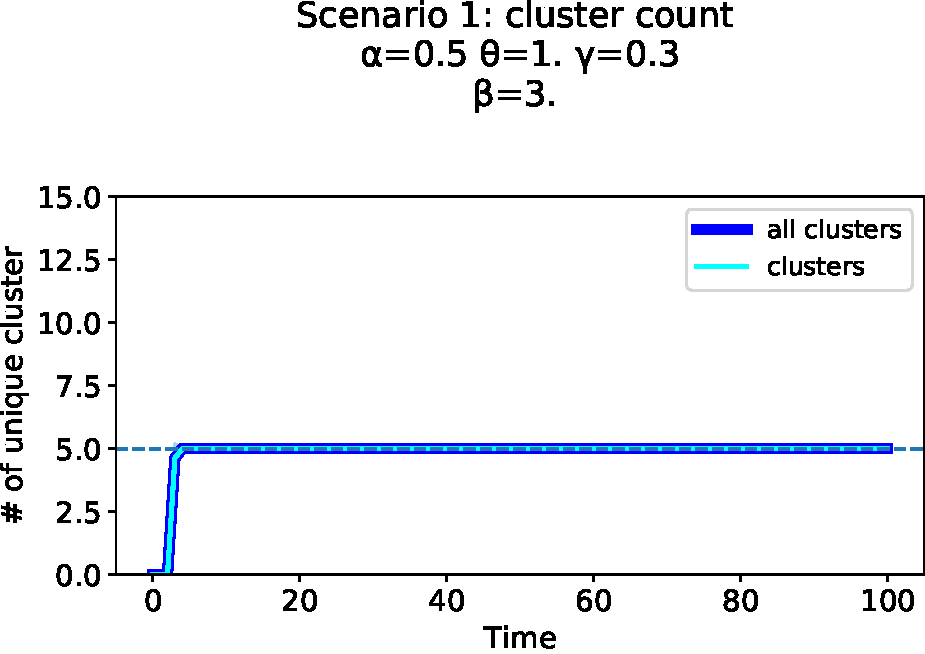
\includegraphics[width=\textwidth]{papers/swarm-intelligence2021/img/simulations/standard_cluster_count.pdf}
  \end{subfigure}
  \hfill
  \centering
  %%% Scenario 2 %%%
  \begin{subfigure}[b]{0.32\textwidth}
    \centering
    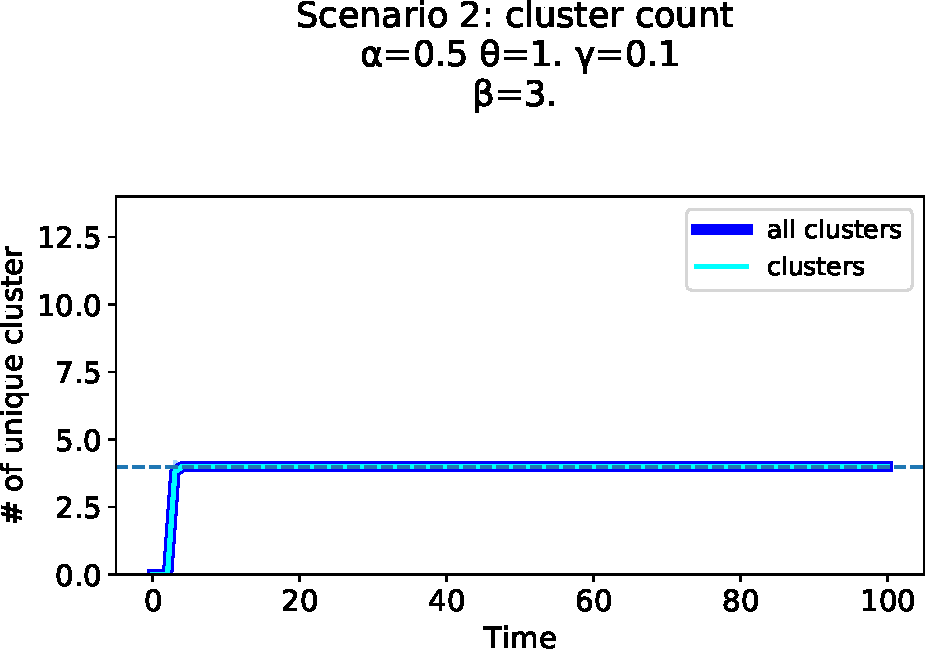
\includegraphics[width=\textwidth]{papers/swarm-intelligence2021/img/simulations/stretched_cluster_count.pdf}
  \end{subfigure}
  \hfill
  \centering
  %%% Scenario 3 %%%
  \begin{subfigure}[b]{0.32\textwidth}
    \centering
    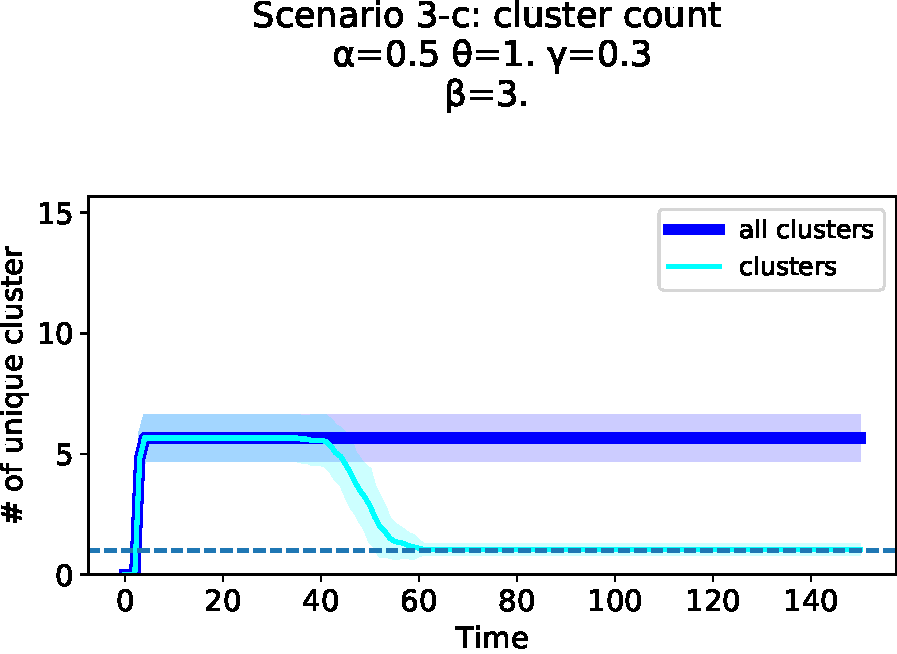
\includegraphics[width=\textwidth]{papers/swarm-intelligence2021/img/simulations/one-direction_0_021_α-0.5_θ-1._γ-0.3_β-3._ω-0._ζ-0..pdf}
  \end{subfigure}
  \hfill
  \centering
  %%% Scenario 4 %%%
  \begin{subfigure}[b]{0.32\textwidth}
    \centering
    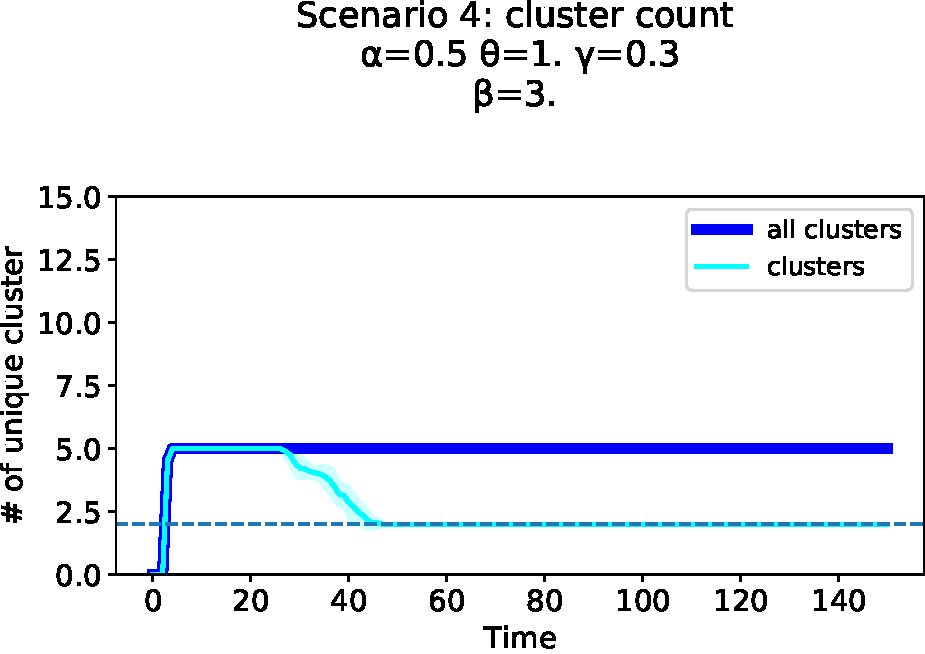
\includegraphics[width=\textwidth]{papers/swarm-intelligence2021/img/simulations/overlay_0_021_α-0.5_θ-1._γ-0.3_β-3._ω-0._ζ-0..pdf}
  \end{subfigure}
  \hfill
  \centering
  %%% Scenario 5 %%%
  \begin{subfigure}[b]{0.32\textwidth}
    \centering
    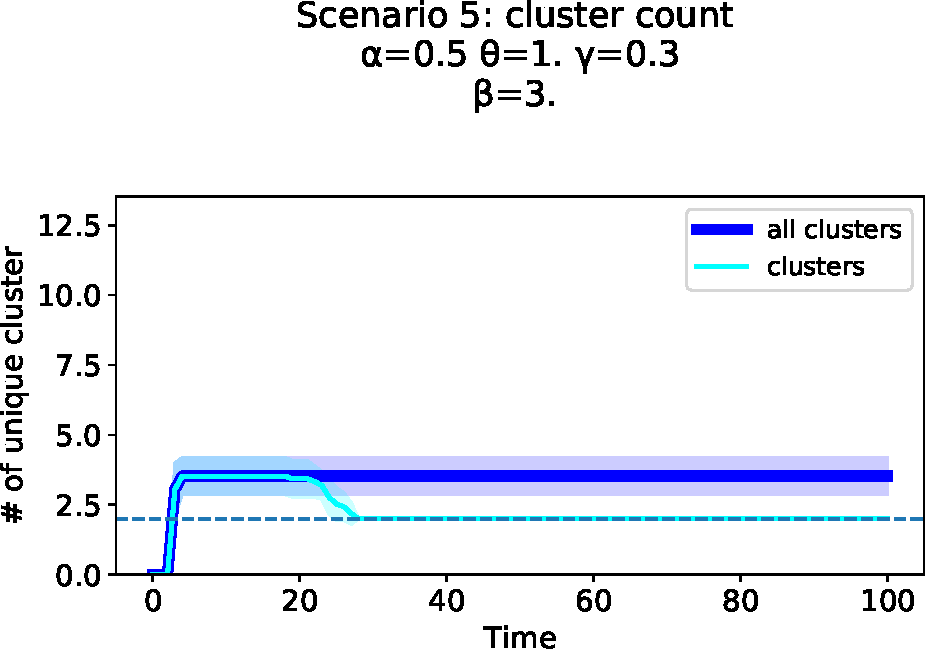
\includegraphics[width=\textwidth]{papers/swarm-intelligence2021/img/simulations/non-convex_0_021_α-0.5_θ-1._γ-0.3_β-3._ω-0._ζ-0..pdf}
  \end{subfigure}
  \hfill
  \centering
  %%% Scenario 6 %%%
  \begin{subfigure}[b]{0.32\textwidth}
    \centering
    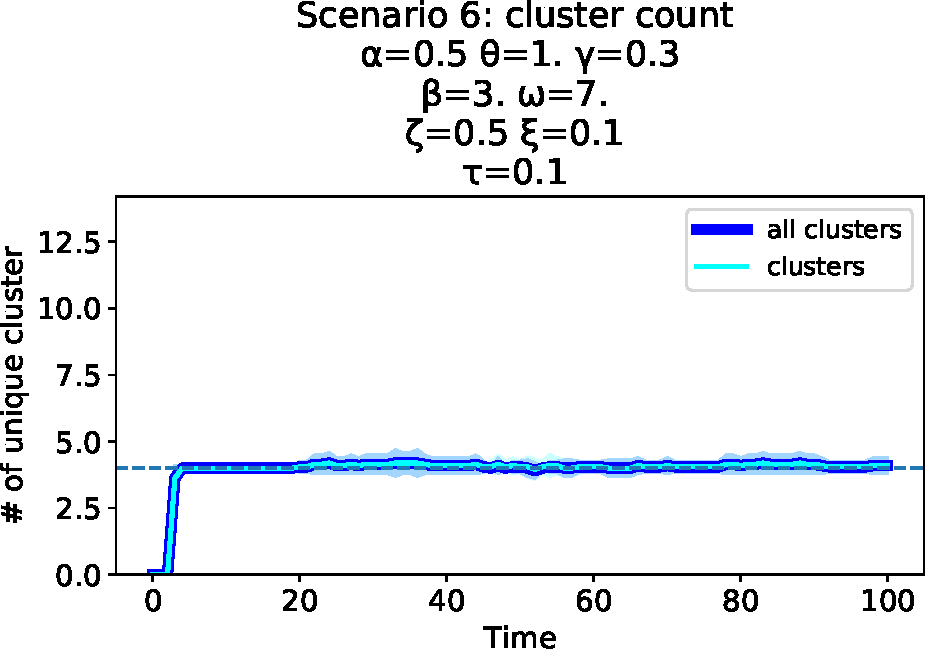
\includegraphics[width=\textwidth]{papers/swarm-intelligence2021/img/simulations/movement_cluster_count.pdf}
  \end{subfigure}
  \centering
  %%% Scenario 7 %%%
  \begin{subfigure}[b]{0.32\textwidth}
    \centering
    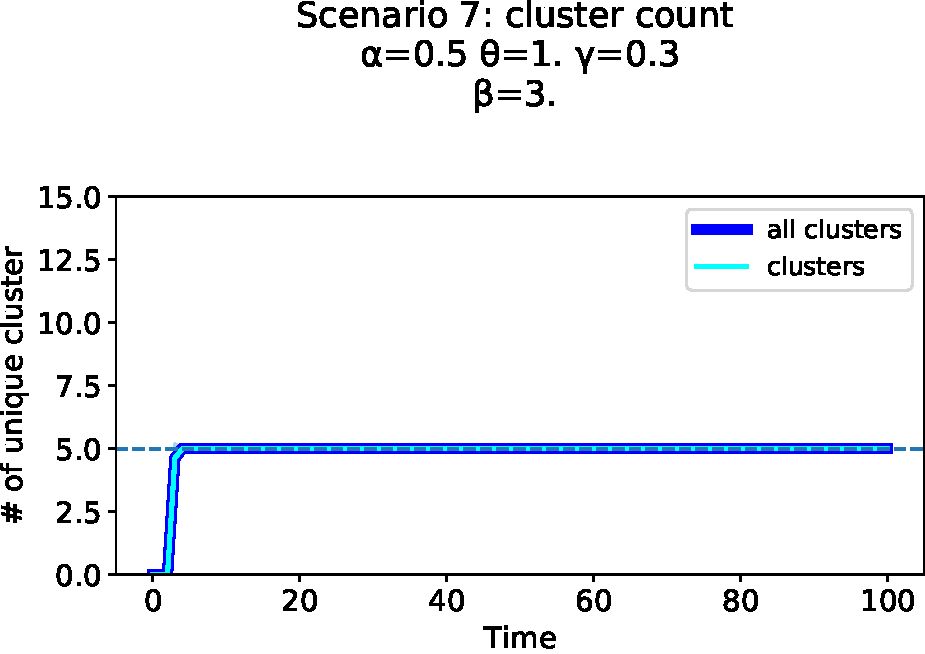
\includegraphics[width=\textwidth]{papers/swarm-intelligence2021/img/simulations/standard-updatable_0_021_α-0.5_θ-1._γ-0.3_β-3._ω-0._ζ-0..pdf}
  \end{subfigure}
  %%% Scenario 8 %%%
  \begin{subfigure}[b]{0.32\textwidth}
    \centering
    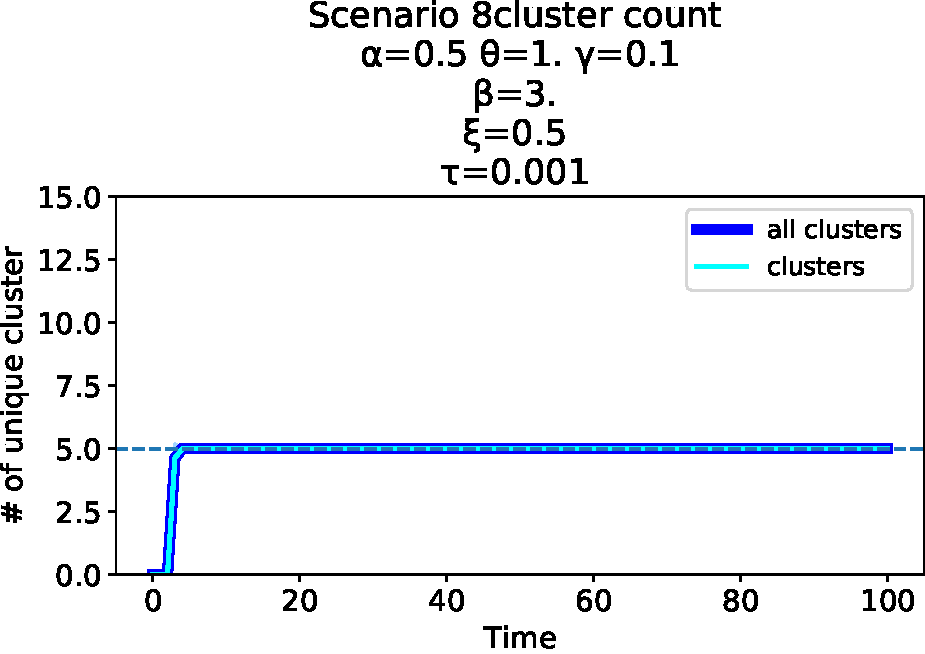
\includegraphics[width=\textwidth]{papers/swarm-intelligence2021/img/simulations/failScenario_0_021_α-0.5_θ-1._γ-0.1_β-3._ω-0._ζ-0._ξ-0.5_τ-0.001}
  \end{subfigure}
  \caption[Overview of simulation results in different clustering scenarios]{Overview of simulation results. 
  The dotted lines identify the ideal cluster division count. 
  The blue lines show the unique cluster found. 
  Instead, the cyan lines indicate the unique cluster number after the merging phase. 
  %In each scenario, the algorithm eventually reaches the correct cluster division count. 
  }
  \label{fig:overview-results}
\end{figure}
\begin{figure}[!ht]
  \begin{subfigure}[b]{0.32\textwidth}
    \centering
    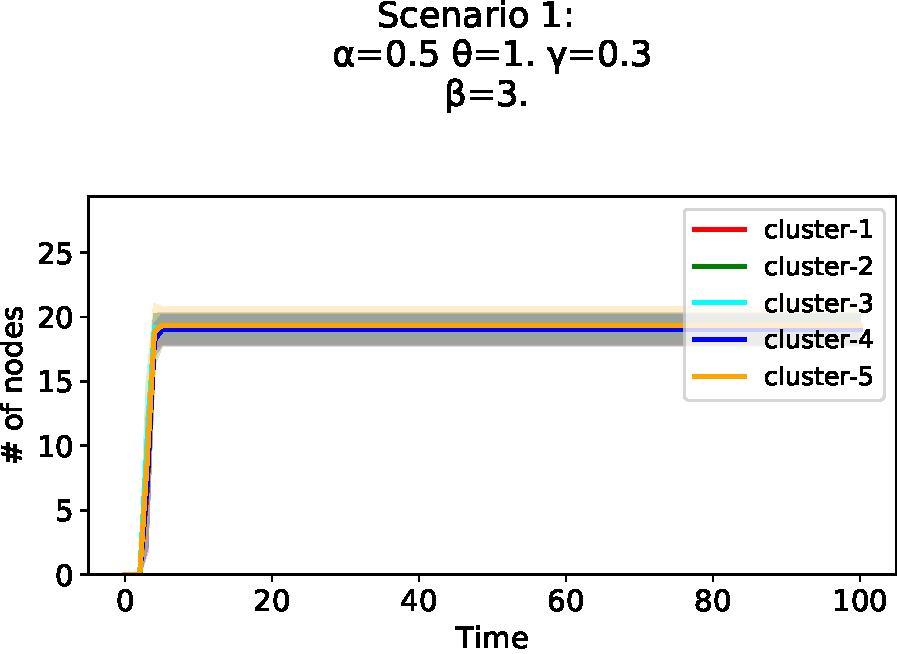
\includegraphics[width=\textwidth]{papers/swarm-intelligence2021/img/simulations/standard-count_0_034567_α-0.5_θ-1._γ-0.3_β-3._ω-0._ζ-0..pdf}
  \end{subfigure}
  \hfill
  \begin{subfigure}[b]{0.32\textwidth}
    \centering
    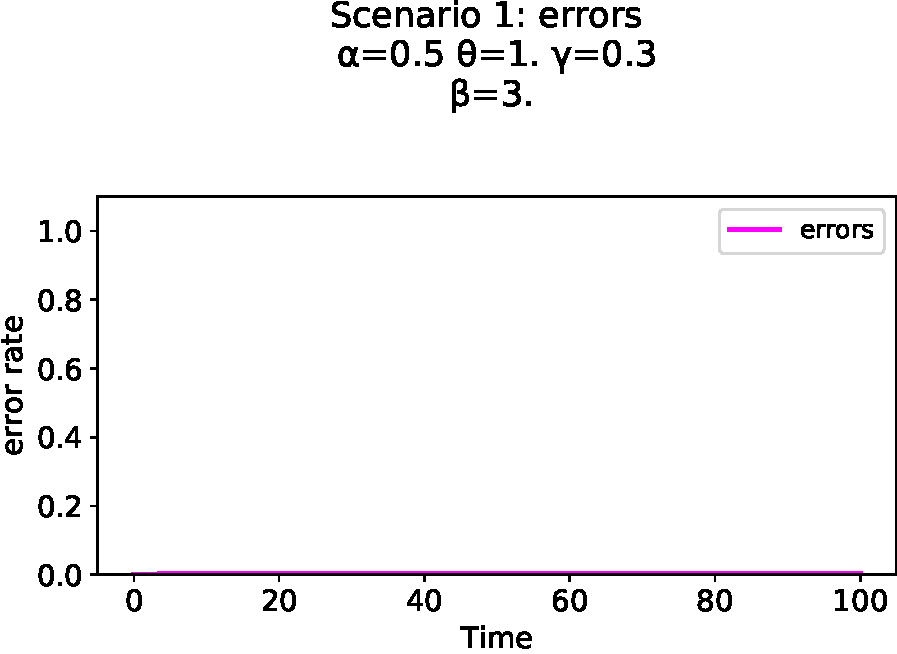
\includegraphics[width=\textwidth]{papers/swarm-intelligence2021/img/simulations/standard-errors_0_08_α-0.5_θ-1._γ-0.3_β-3._ω-0._ζ-0..pdf}
  \end{subfigure}
  \hfill
  \begin{subfigure}[b]{0.32\textwidth}
    \centering
    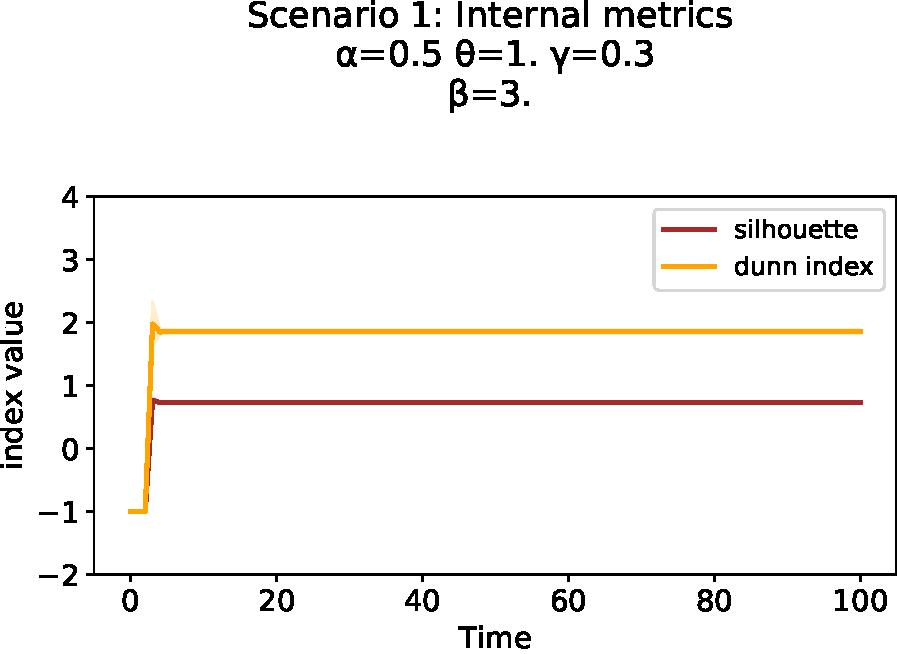
\includegraphics[width=\textwidth]{papers/swarm-intelligence2021/img/simulations/standard-metrics_0_0910_α-0.5_θ-1._γ-0.3_β-3._ω-0._ζ-0..pdf}
  \end{subfigure}
  \\
  \begin{subfigure}[b]{0.32\textwidth}
    \centering
    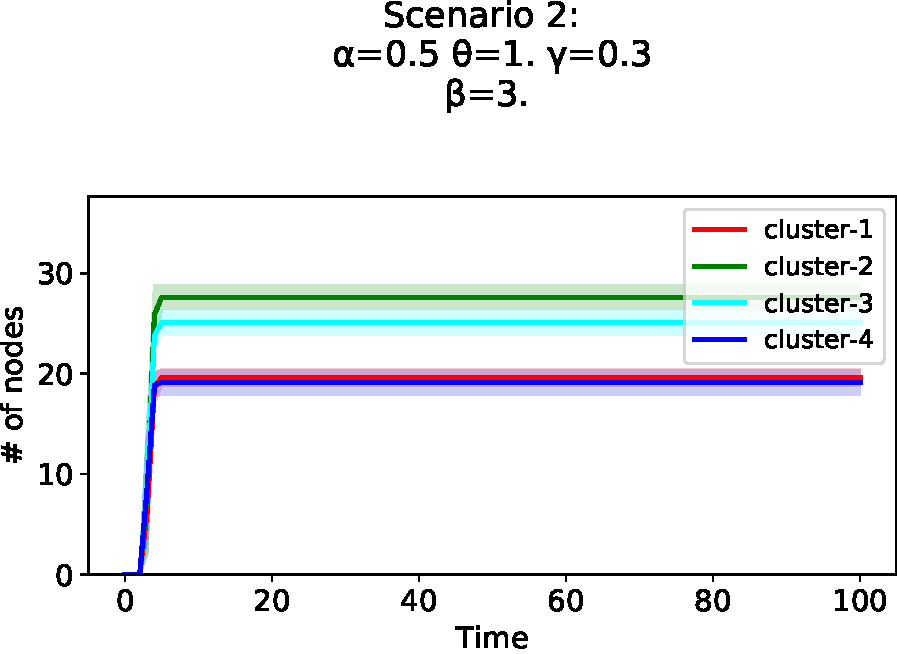
\includegraphics[width=\textwidth]{papers/swarm-intelligence2021/img/simulations/stretched-count_0_03456_α-0.5_θ-1._γ-0.3_β-3._ω-0._ζ-0..pdf}
  \end{subfigure}
  \hfill
  \begin{subfigure}[b]{0.32\textwidth}
    \centering
    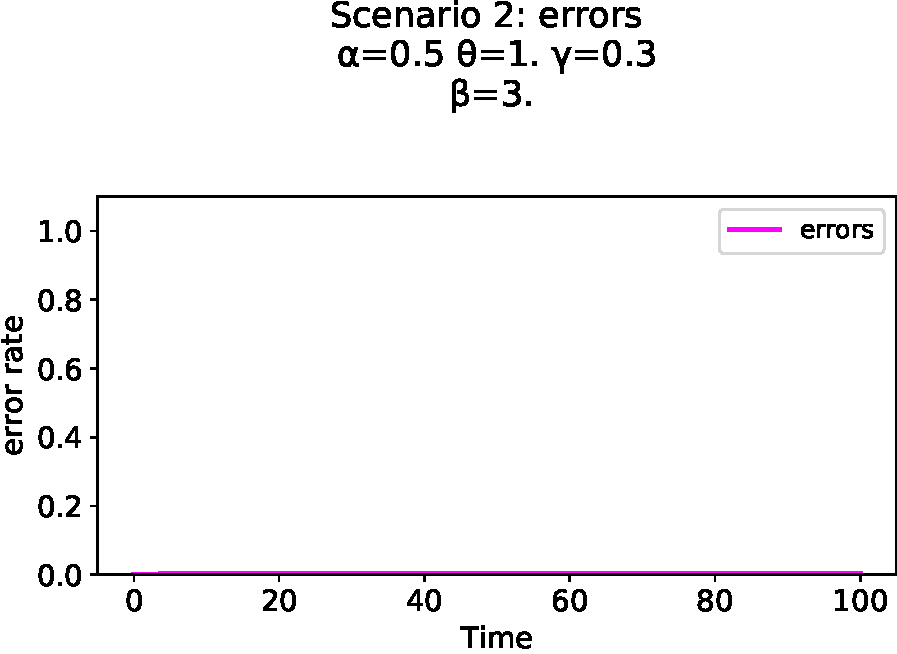
\includegraphics[width=\textwidth]{papers/swarm-intelligence2021/img/simulations/stretched-errors_0_08_α-0.5_θ-1._γ-0.3_β-3._ω-0._ζ-0..pdf}
  \end{subfigure}
  \hfill
  \begin{subfigure}[b]{0.32\textwidth}
    \centering
    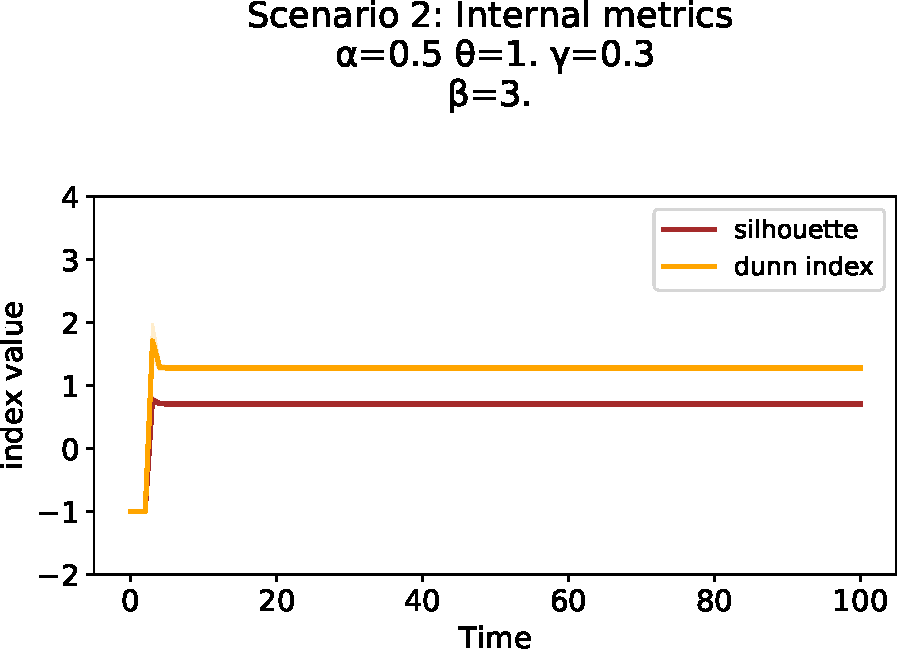
\includegraphics[width=\textwidth]{papers/swarm-intelligence2021/img/simulations/stretched-metrics_0_0910_α-0.5_θ-1._γ-0.3_β-3._ω-0._ζ-0..pdf}
  \end{subfigure}
  \\
  \begin{subfigure}[b]{0.32\textwidth}
    \centering
    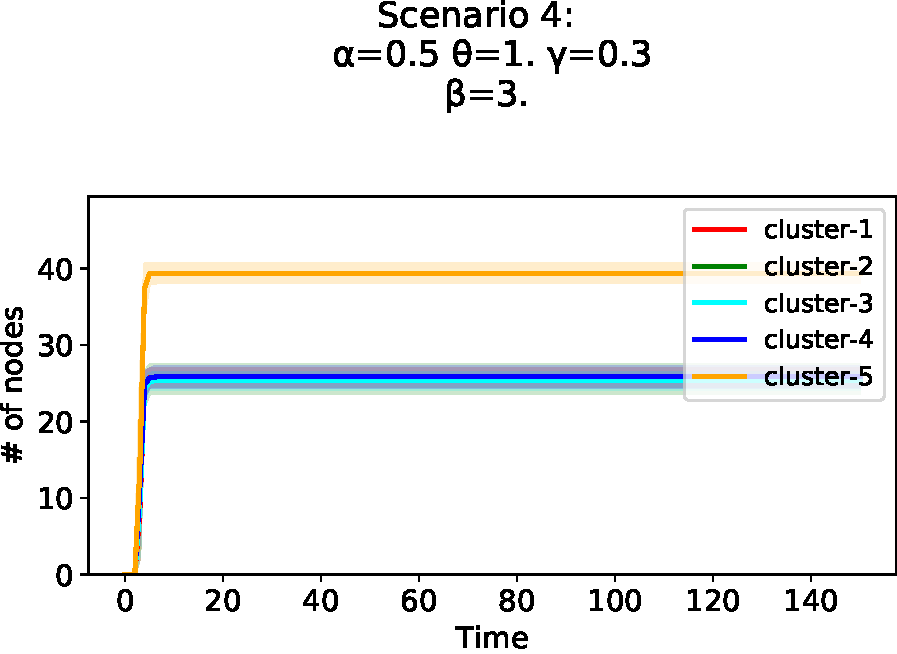
\includegraphics[width=\textwidth]{papers/swarm-intelligence2021/img/simulations/overlay-count_0_034567_α-0.5_θ-1._γ-0.3_β-3._ω-0._ζ-0..pdf}
  \end{subfigure}
  \hfill
  \begin{subfigure}[b]{0.32\textwidth}
    \centering
    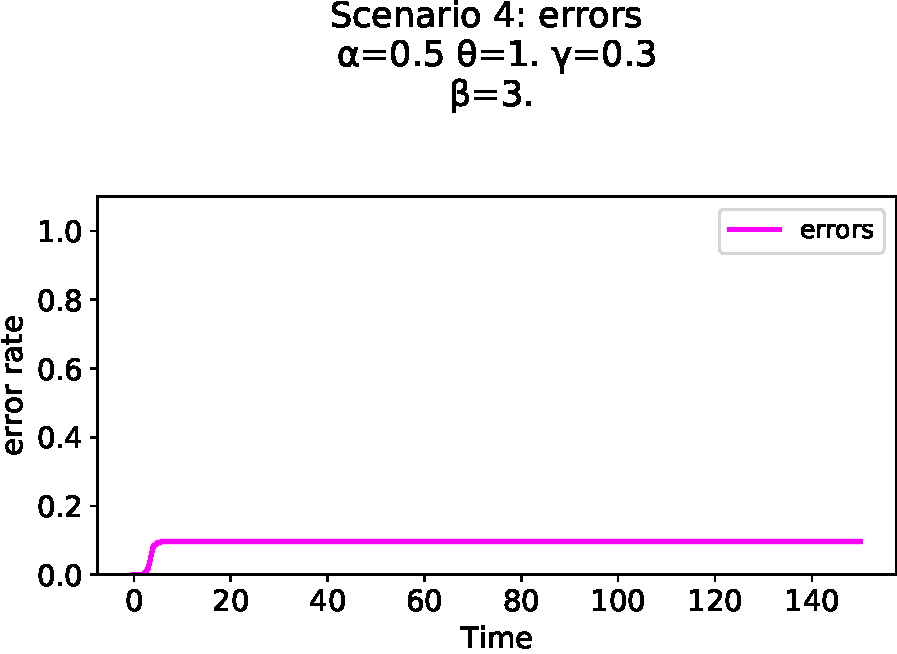
\includegraphics[width=\textwidth]{papers/swarm-intelligence2021/img/simulations/overlay-errors_0_08_α-0.5_θ-1._γ-0.3_β-3._ω-0._ζ-0..pdf}
  \end{subfigure}
  \hfill
  \begin{subfigure}[b]{0.32\textwidth}
    \centering
    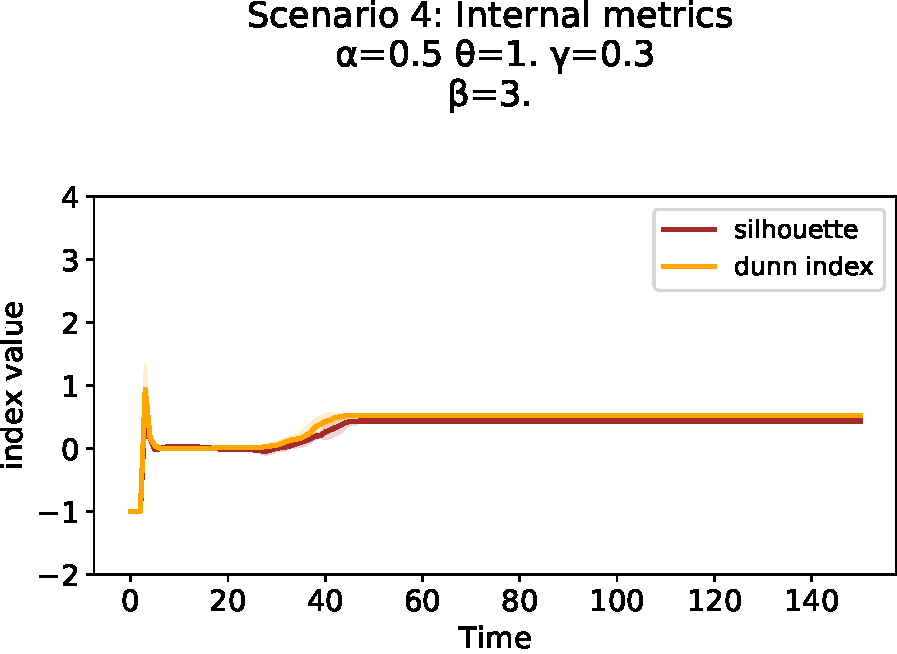
\includegraphics[width=\textwidth]{papers/swarm-intelligence2021/img/simulations/overlay-metrics_0_0910_α-0.5_θ-1._γ-0.3_β-3._ω-0._ζ-0..pdf}
  \end{subfigure}
  \\
  \begin{subfigure}[b]{0.32\textwidth}
    \centering
    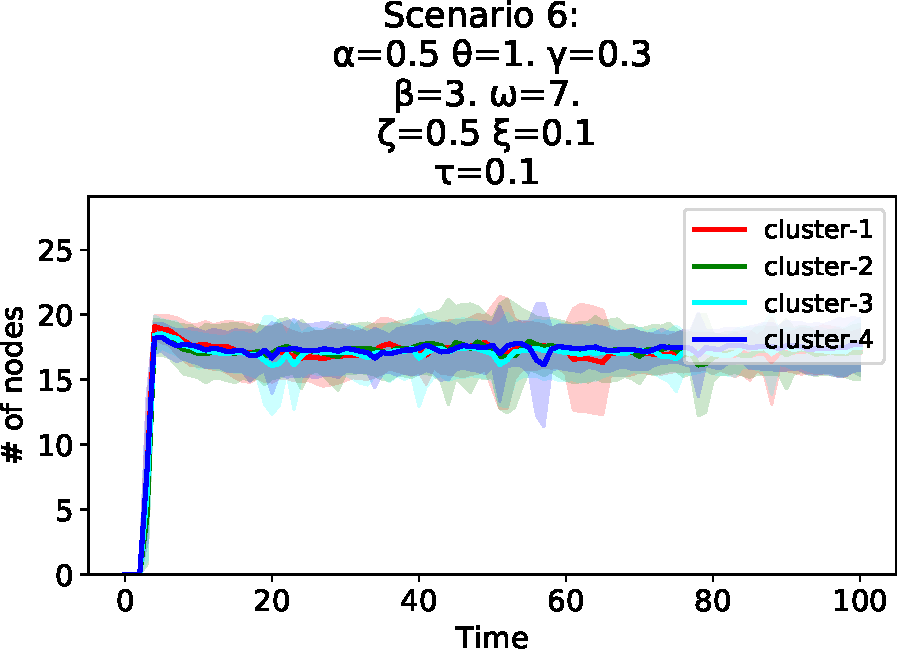
\includegraphics[width=\textwidth]{papers/swarm-intelligence2021/img/simulations/movement-count_0_03456_α-0.5_θ-1._γ-0.3_β-3._ω-7._ζ-0.5.pdf}
  \end{subfigure}
  \hfill
  \begin{subfigure}[b]{0.32\textwidth}
    \centering
    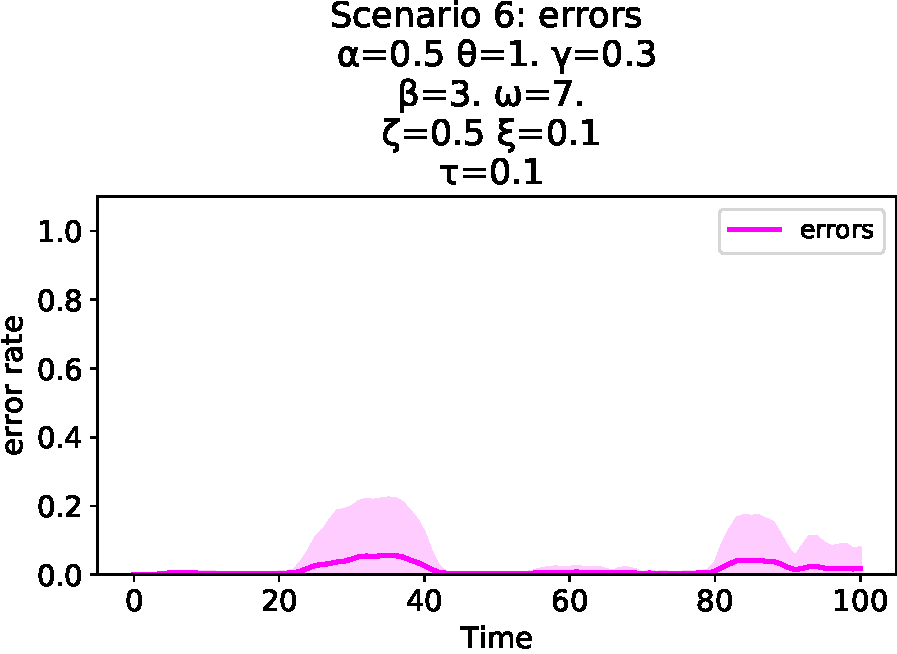
\includegraphics[width=\textwidth]{papers/swarm-intelligence2021/img/simulations/movement-errors_0_08_α-0.5_θ-1._γ-0.3_β-3._ω-7._ζ-0.5.pdf}
  \end{subfigure}
  \hfill
  \begin{subfigure}[b]{0.32\textwidth}
    \centering
    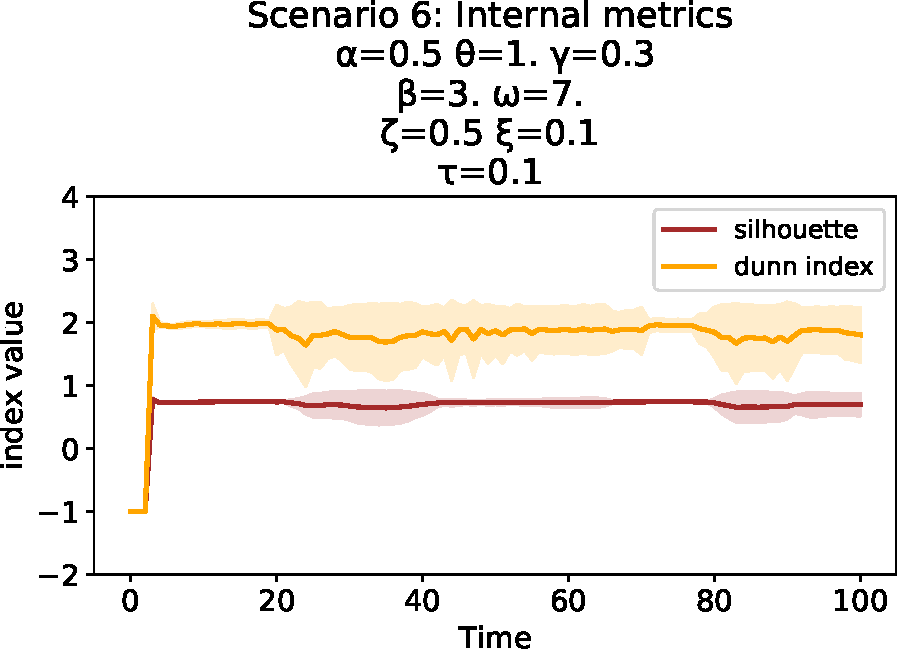
\includegraphics[width=\textwidth]{papers/swarm-intelligence2021/img/simulations/movement-metrics_0_0910_α-0.5_θ-1._γ-0.3_β-3._ω-7._ζ-0.5.pdf}
  \end{subfigure}
  \\
  \begin{subfigure}[b]{0.32\textwidth}
    \centering
    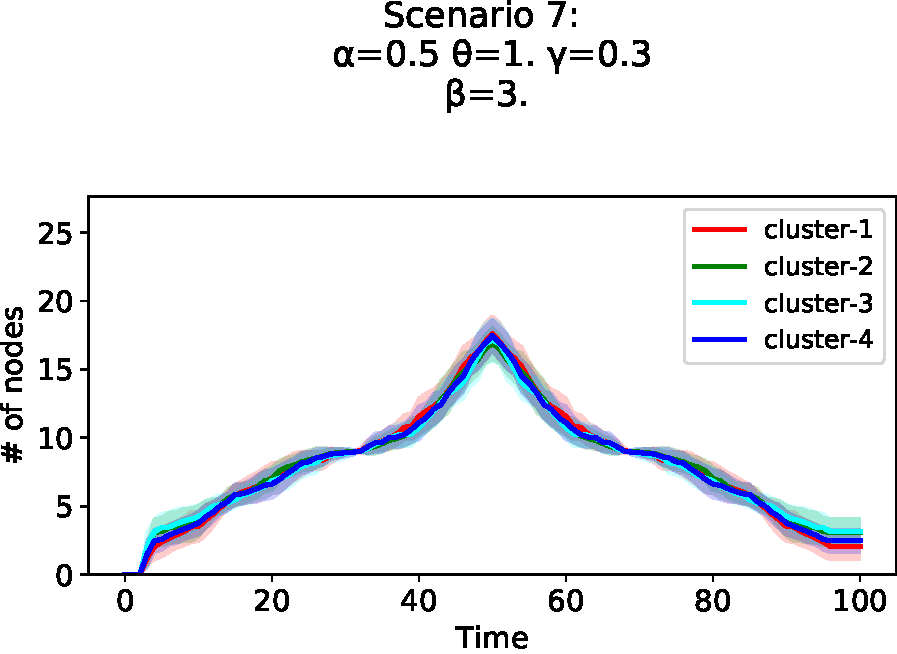
\includegraphics[width=\textwidth]{papers/swarm-intelligence2021/img/simulations/standard-updatable-count_0_03456_α-0.5_θ-1._γ-0.3_β-3._ω-0._ζ-0..pdf}
  \end{subfigure}
  \hfill
  \begin{subfigure}[b]{0.32\textwidth}
    \centering
    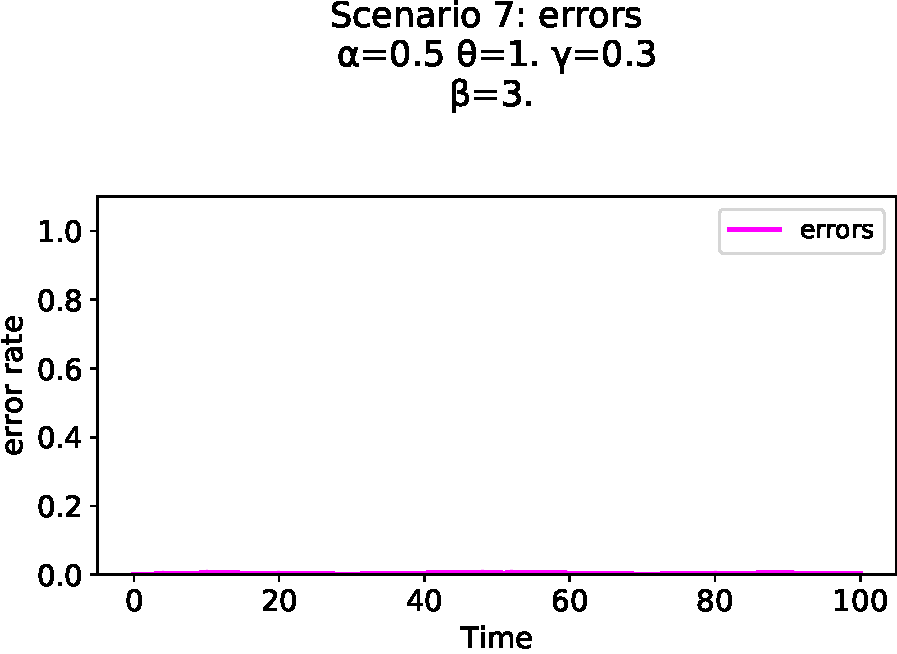
\includegraphics[width=\textwidth]{papers/swarm-intelligence2021/img/simulations/standard-updatable-errors_0_08_α-0.5_θ-1._γ-0.3_β-3._ω-0._ζ-0..pdf}
  \end{subfigure}
  \hfill
  \begin{subfigure}[b]{0.32\textwidth}
    \centering
    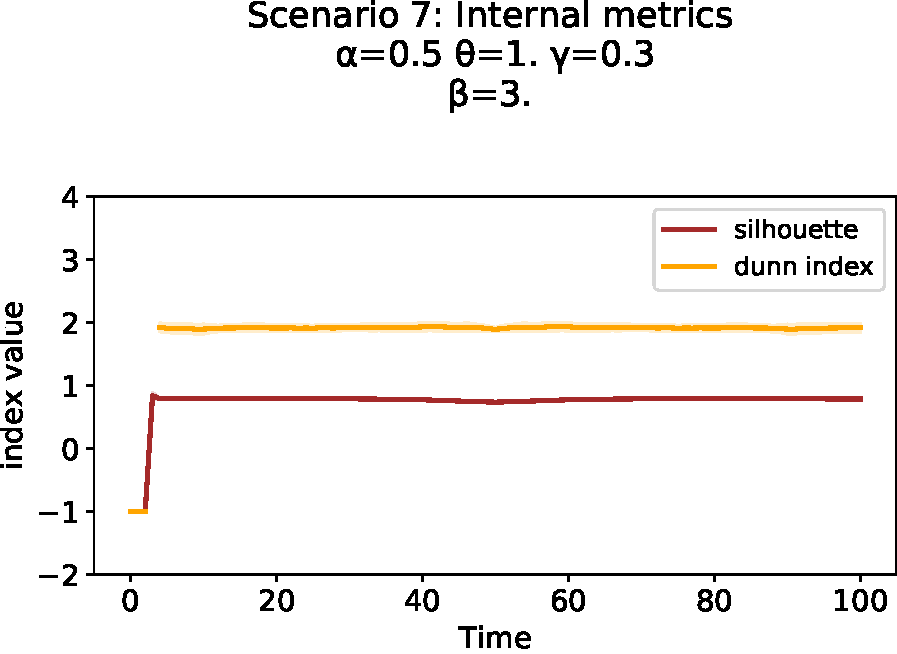
\includegraphics[width=\textwidth]{papers/swarm-intelligence2021/img/simulations/standard-updatable-metrics_0_0910_α-0.5_θ-1._γ-0.3_β-3._ω-0._ζ-0..pdf}
  \end{subfigure}
  \\
  \begin{subfigure}[b]{0.32\textwidth}
    \centering
    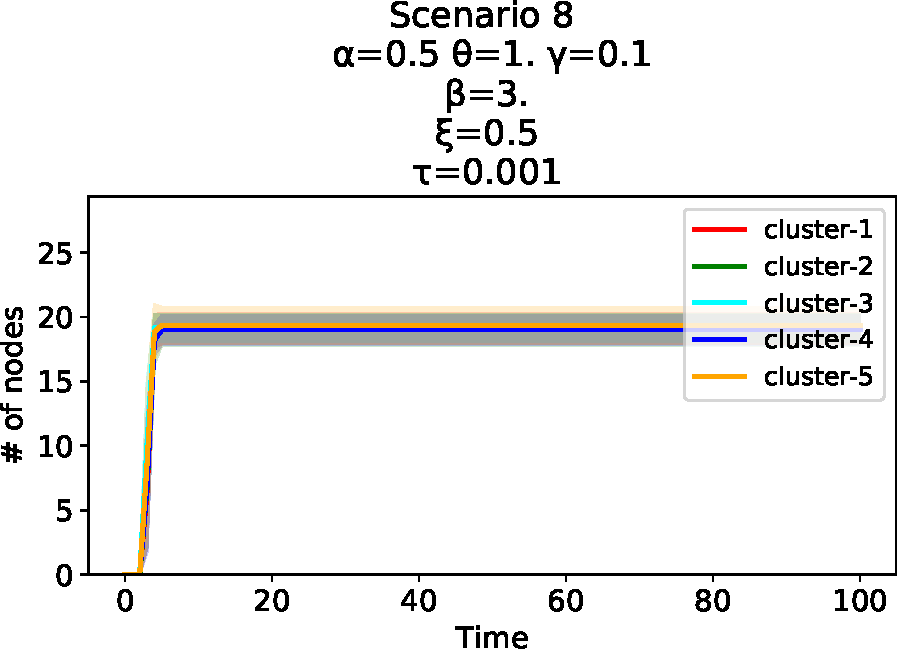
\includegraphics[width=\textwidth]{papers/swarm-intelligence2021/img/simulations/failScenario_0_034567_α-0.5_θ-1._γ-0.1_β-3._ω-0._ζ-0._ξ-0.5_τ-0.001}
  \end{subfigure}
  \hfill
  \begin{subfigure}[b]{0.32\textwidth}
    \centering
    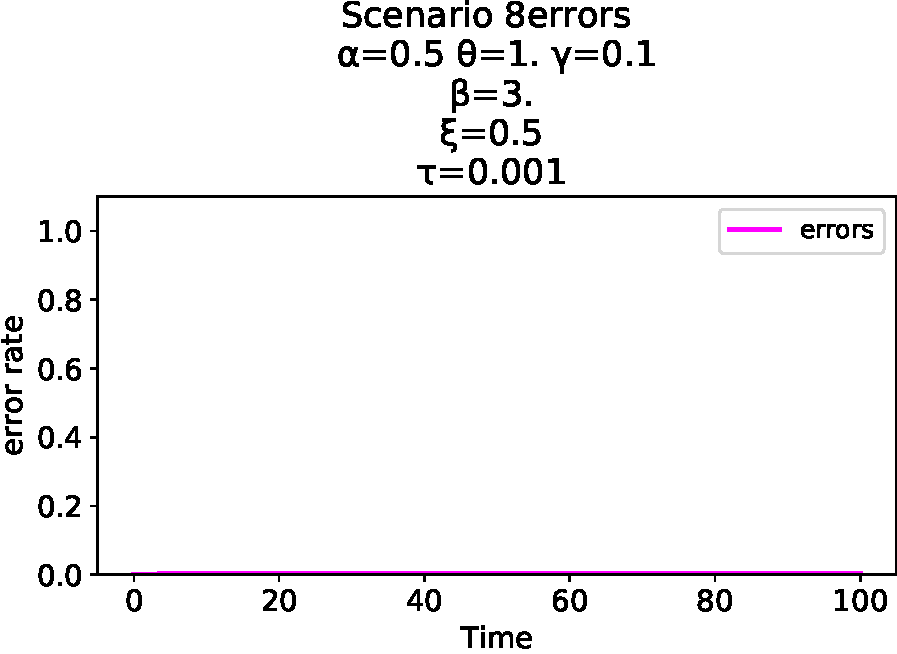
\includegraphics[width=\textwidth]{papers/swarm-intelligence2021/img/simulations/failScenario_0_08_α-0.5_θ-1._γ-0.1_β-3._ω-0._ζ-0._ξ-0.5_τ-0.001}
  \end{subfigure}
  \hfill
  \begin{subfigure}[b]{0.32\textwidth}
    \centering
    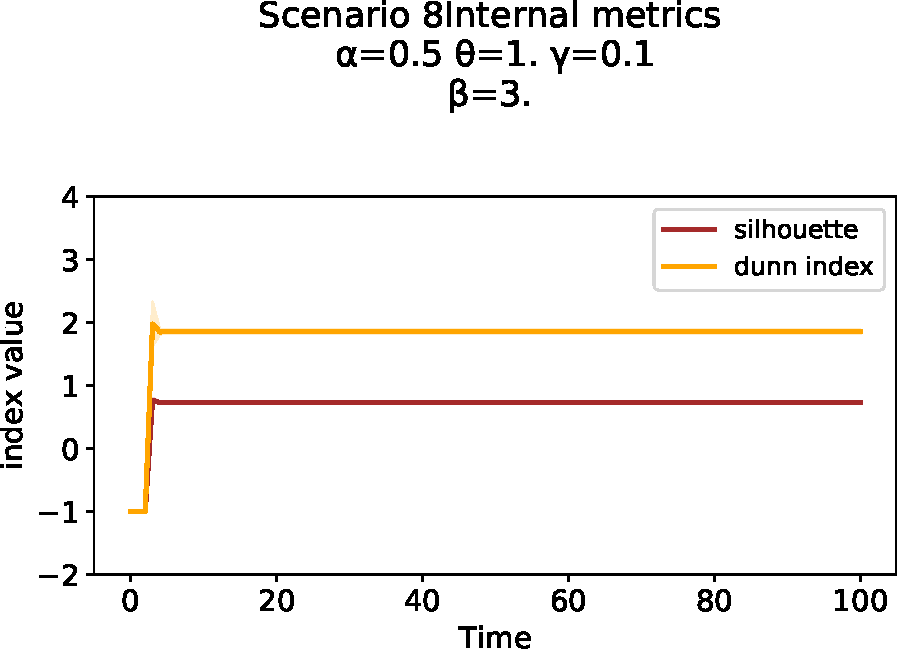
\includegraphics[width=\textwidth]{papers/swarm-intelligence2021/img/simulations/failScenario_0_0910_α-0.5_θ-1._γ-0.1_β-3._ω-0._ζ-0._ξ-0.5_τ-0.001}
  \end{subfigure}
  \caption{In-depth analysis of good simulation results. 
  In general, the algorithm produces good results. 
  \rev{In the case of movement and failures, the error can reach up to 10 per cent.}}
  
  \label{fig:good-simulation-results}
\end{figure}

\begin{figure}[!ht]
  %%% PROBLEM 1: thr %%% 
  \begin{subfigure}[b]{0.32\textwidth}
    \centering
    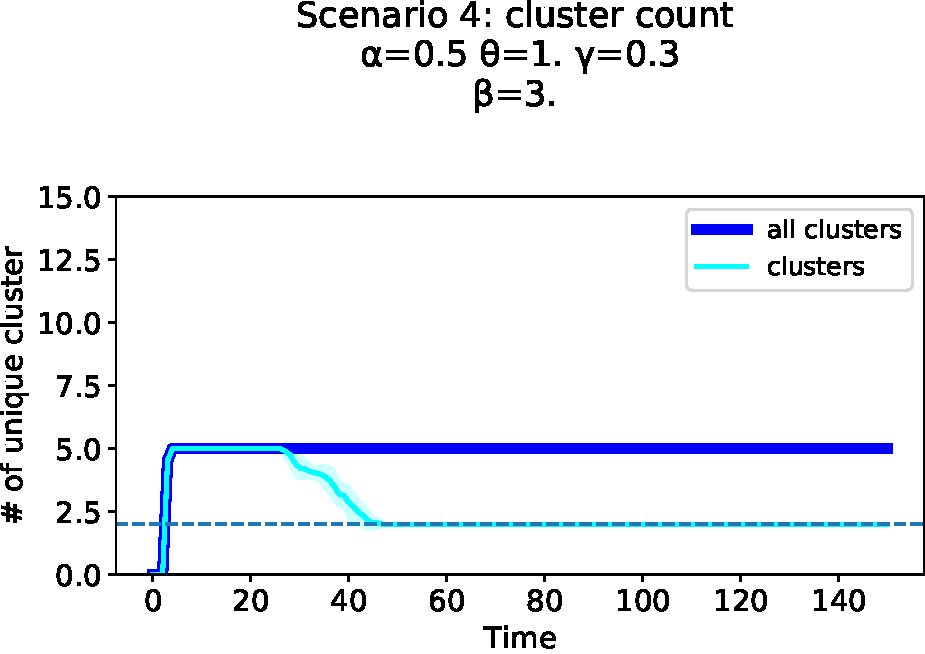
\includegraphics[width=\textwidth]{papers/swarm-intelligence2021/img/simulations/overlay_0_021_α-0.5_θ-1._γ-0.3_β-3._ω-0._ζ-0..pdf}
  \end{subfigure}
  \hfill
  \begin{subfigure}[b]{0.32\textwidth}
    \centering
    \includegraphics[width=\textwidth]{papers/swarm-intelligence2021/img/simulations/overlay_0_021_α-0.5_θ-1.5_γ-0.3_β-3._ω-0._ζ-0..pdf}
  \end{subfigure}
  \hfill
  \begin{subfigure}[b]{0.32\textwidth}
    \centering
    \includegraphics[width=\textwidth]{papers/swarm-intelligence2021/img/simulations/overlay_0_021_α-0.5_θ-0.5_γ-0.3_β-3._ω-0._ζ-0..pdf}
  \end{subfigure}
  %%% PROBLEM 2: density %%% 
  \begin{subfigure}[b]{0.32\textwidth}
    \centering
    \includegraphics[width=\textwidth]{papers/swarm-intelligence2021/img/simulations/standard-updatable-errors_0_08_α-0.75_θ-0.5_γ-0.1_β-5._ω-0._ζ-0..pdf}
  \end{subfigure}
  \hfill
  \begin{subfigure}[b]{0.32\textwidth}
    \centering
    \includegraphics[width=\textwidth]{papers/swarm-intelligence2021/img/simulations/standard-errors_0_08_α-0.75_θ-1.5_γ-0.1_β-7._ω-0._ζ-0..pdf}
  \end{subfigure}
  \hfill
  \begin{subfigure}[b]{0.32\textwidth}
    \centering
    \includegraphics[width=\textwidth]{papers/swarm-intelligence2021/img/simulations/stretched-errors_0_08_α-0.75_θ-1.5_γ-0.3_β-5._ω-0._ζ-0..pdf}
  \end{subfigure}
  \\
  %% Focus 3: mobility
  \begin{subfigure}[b]{0.32\textwidth}
    \centering
    \includegraphics[width=\textwidth]{papers/swarm-intelligence2021/img/simulations/movement-errors_0_08_α-0.5_θ-1._γ-0.3_β-3._ω-7._ζ-0.5.pdf}
  \end{subfigure}
  \hfill
  \begin{subfigure}[b]{0.32\textwidth}
    \centering
    \includegraphics[width=\textwidth]{papers/swarm-intelligence2021/img/simulations/movement-errors_0_08_α-0.5_θ-1._γ-0.3_β-3._ω-10._ζ-0.5.pdf}
  \end{subfigure}
  \hfill
  \begin{subfigure}[b]{0.32\textwidth}
    \centering
    \includegraphics[width=\textwidth]{papers/swarm-intelligence2021/img/simulations/movement-errors_0_08_α-0.5_θ-1._γ-0.3_β-3._ω-14._ζ-0.5.pdf}
  \end{subfigure}
  \\
  %% Focus 4: movement range
  \begin{subfigure}[b]{0.32\textwidth}
    \centering
    \includegraphics[width=\textwidth]{papers/swarm-intelligence2021/img/simulations/movement-errors_0_08_α-0.5_θ-1.5_γ-0.1_β-3._ω-7._ζ-0.6.pdf}
  \end{subfigure}
  \hfill
  \begin{subfigure}[b]{0.32\textwidth}
    \centering
    \includegraphics[width=\textwidth]{papers/swarm-intelligence2021/img/simulations/movement-errors_0_08_α-0.5_θ-1._γ-0.1_β-3._ω-7._ζ-0.6.pdf}
  \end{subfigure}
  \hfill
  \begin{subfigure}[b]{0.32\textwidth}
    \centering
    \includegraphics[width=\textwidth]{papers/swarm-intelligence2021/img/simulations/movement-errors_0_08_α-0.5_θ-1._γ-0.7_β-3._ω-10._ζ-0.6.pdf}
  \end{subfigure}
  %% Focus 4: movement range
  \begin{subfigure}[b]{0.32\textwidth}
    \centering
    \includegraphics[width=\textwidth]{papers/swarm-intelligence2021/img/simulations/failScenario_0_08_α-0.75_θ-0.5_γ-0.1_β-7._ω-0._ζ-0._ξ-0.5_τ-0.001}
  \end{subfigure}
  \hfill
  \begin{subfigure}[b]{0.32\textwidth}
    \centering
    \includegraphics[width=\textwidth]{papers/swarm-intelligence2021/img/simulations/failScenario_0_08_α-0.75_θ-0.5_γ-0.1_β-7._ω-0._ζ-0._ξ-0.5_τ-0.1}
  \end{subfigure}
  \hfill
  \begin{subfigure}[b]{0.32\textwidth}
    \centering
    \includegraphics[width=\textwidth]{papers/swarm-intelligence2021/img/simulations/failScenario_0_08_α-0.75_θ-0.5_γ-0.1_β-7._ω-0._ζ-0._ξ-0.5_τ-0.5}
  \end{subfigure}
  \caption{Main examples of bad clustering results.
  In the first line, the images show different behaviour varying $\theta$.
  In the second line, the plots show how the algorithm does not handle well low-density robot swarms.
  In the third line, the charts show how the algorithm handles various movement speeds.
  The fourth line shows how the exploration range impacts the clustering results.
  \rev{Finally, the last line shows how failures impact performance.}
  }
  \label{fig:bad-simulation-results}
\end{figure}
The simulation results underscore the algorithm's capability to effectively partition the data into meaningful clusters. 
 As demonstrated in \Cref{fig:overview-results}, 
 our algorithm stabilizes to produce the correct number of clusters after a certain settling period. 
In the sections that follow, we concentrate on discussing the outcomes in relation to the evaluation goals outlined in \Cref{s:eval-goal}.
\paragraph*{Goal \ref{goal:1}: static sensing/spatial-based clustering}
Running the simulations of scenarios 1-5 we verified how much the clusters extracted follow the underlying temperature distribution in the static context.
 \Cref{fig:overview-results} shows that the algorithm correctly extracts the cluster number -- with the optimal parameters' configuration.
 Furthermore, observing \Cref{fig:good-simulation-results}, we can deduce that the cluster shape is correct too.
 Indeed, the Silhouette index tends to be 1 when the clusters are disjointed, and the error rate is negligible.

Here, $\theta$ plays a key role. Observing the behaviour of scenario 4 in \Cref{fig:bad-simulation-results},
 we see that with too low $\theta$ we overestimate the cluster numbers and,
 with a high level of $\theta$, we underestimate the cluster number.
 But this was the expected behaviour, as it depends directly on the trend of the target distributions.

Finally, Another important aspect is the density ($\alpha$) of the system.
 With a few nodes, candidate nodes may be positioned far from the cluster centre, thus identifying wider areas than expected.
\paragraph*{Goal \ref{goal:2}: robustness against node mobility \emph{and failures}}
When nodes have a low mobility and exploration range, the system is robust to node movements (\Cref{fig:good-simulation-results}).
 The exploring policy introduces errors, but the results are comparable to solutions where the nodes are stationary.
Moreover, even in case of failures, the clustering process is practically not affected at all.
However, in the worst case, mobility and failures lead to false positives (\Cref{fig:bad-simulation-results}).
 Indeed, some processes start in areas where the temperature is almost constant.
 Therefore, that process approximately covers the whole area (and hence produces a high error rate).
\rev{Scenario 8 is mainly influenced by the low-density situation.
 Indeed, in that case, removing nodes lead to not covering the whole system. }
\paragraph*{Goal \ref{goal:3}: robustness against temperature changes}
The result of scenario 7 is comparable to the static scenario.
 Indeed, \Cref{fig:good-simulation-results} shows that the cluster number is correct, and \Cref{fig:good-simulation-results} shows that the error rate is low, and the shape is accurate.
 The solution suffers from low-density values and wrong $\theta$ values as scenarios 1-5 (\Cref{fig:bad-simulation-results}).

\subsection{Discussion}
\label{sec:eval-discussion}

\rev{\subsubsection*{Simulations} \label{sec:eval-discussion-simulations}}
Ultimately, 
 our algorithm can support a certain degree of movement, \rev{sporadic failures},
 find various cluster shapes, 
 and cope with temperature changes in the optimal condition:
 high density ($\alpha$), limited exploration range ($\zeta$), and an appropriate value for in cluster threshold ($\theta$) value.

However, when drones move randomly, 
 the algorithm starts to produce sub-optimal cluster divisions since the nodes do not care about the cluster found,
 and they continue to explore the area.
%
But this could lead to becoming a false candidate and then starting an unwanted clustering process.
 Furthermore, it could be argued that uniform zones are part of a cluster that is not identified as there are no relative minima.
%
For this reason, when a node starts the process in a non-correct zone, the cluster identification will expand in the nearly whole system.
 This problem could be reduced by changing $\omega$ and $\zeta$ when the nodes belong to a cluster.

It is important to highlight that when \(\alpha\) is set to a low value, 
 the algorithm tends to produce poor cluster divisions, a phenomenon that becomes particularly evident in the presence of failures. 
 This limitation is inherent to our algorithm's design, 
 which relies on a centroid to initiate the clustering process.
% 
With a low \(\alpha\) value, 
 the likelihood increases that the node initiating the clustering process is distant from the true centroid of the cluster. 
 As a result, the expansion process may deviate from the underlying distribution, leading to a significant misclassification of nodes.

\subsubsection*{Hardware Deployment}
\label{sec:eval-discussion-deployment}
While we have not conducted experiments involving the clustering algorithm on a physical system, 
 insights can be gleaned from the physical deployment of FCPP~\cite{DBLP:conf/acsos/Audrito20}, a C++ library that provides an internal DSL for field-based programming. 
 This deployment was carried out in the context of an Industrial Internet of Things (IIoT) scenario~\cite{testa:pmcj:2022}. 
 The hardware used consisted of DWM1001C modules by Decawave, which are resource-constrained with a 64MHz ARM Cortex-M4 CPU, 512 KB of flash memory, and 64 KB of RAM. 
 Despite these limitations, the porting of FCPP was successful, and we were able to execute a field-based program with dynamic processes whose complexity is comparable to the clustering algorithm discussed in this paper~\cite{testa:pmcj:2022}.

The DWM1001C modules support BLE (Bluetooth Low Energy) and UWB (Ultra Wideband) for communication. 
 In the IIoT context, BLE was used for message exchange among neighboring nodes, while UWB was employed for distance estimation. 
 This distance data could be integrated into the current clustering algorithm using the \lstinline|gradient| function for multi-hop distance estimation.

Although the FCPP deployment experience has been promising, pointing toward the feasibility of deploying our clustering algorithm in a similar setting, 
 several differences between the two scenarios merit further investigation. 
 Firstly, the largest IIoT experiment involved only 20 nodes, 
 which may be insufficient to adequately assess the clustering algorithm
\section{Related Work}
\label{s:rw}
%
Coverage of related work is organized to separately cover\rev{:
 related swarm-based environment monitoring approaches (\Cref{s:rw:related-env-monitoring}),}
 related clustering models and problems (\Cref{s:rw:related-problems}),
 research work related to the sensing-based clustering problem we address (\Cref{s:rw:related-sensingbased-clustering}),
 research work related to field-based computing (\Cref{s:rw:related-approaches}),
 and related field-based algorithms (\Cref{s:rw:related-ac-algorithms}).

\rev{
\subsection{Swarm-based Environment Monitoring}
\label{s:rw:related-env-monitoring}
%
The approach proposed
 can be used
 to dynamically cluster a swarm,
 e.g.,
 to monitor an environment
 in a decentralized way.
%
Literature on swarm-based environment monitoring
 is ample~\cite{DBLP:journals/ram/DunbabinM12}.
%
In particular, various works leverage mobility and sparse sampling~\cite{DBLP:journals/ijrr/BestCPMF19,casadei2022coord-space-fluid,DBLP:conf/icra/KemnaRNYS17}.

In \cite{DBLP:conf/rss/GargA14},
 a persistent monitoring approach
 of environment phenomena
 with discontinuous dynamics
 is proposed.
%
It is
 based on optimally
 adapting a sparse set of
 sensing locations
 according to an evolving stochastic model of the environment.
%
In~\cite{DBLP:journals/ijrr/BestCPMF19},
 decentralized planning is used to support multi-agent active perception,
  which leverages movement to improve the quality of information gathering through effective choice of ``viewpoints'' in space and time.
%
In~\cite{DBLP:conf/icra/KemnaRNYS17},
 the authors focus on multi-agent coordination for informative adaptive sampling in unknown, communication-constrained environments (like lakes or oceans).
%
Their approach is based on dynamic, 
 decentralized Voronoi partitioning over a set of sampling locations, which are recalculated at synchronization points initiated through requests for surfacing events.
%
Though the approach of this paper could also be used to support \emph{sparse sampling}~\cite{casadei2022coord-space-fluid},
 it also aims at supporting the formation of spatially cohesive clusters for coordinated processing and/or action.
%
Moreover, 
 we do not aim at moving agents to appropriate sampling locations,
 but rather leave the agents to move autonomously (e.g., according to exploration policies)
 while having the collective clustering
 reflect the underlying phenomenon
 to support decision-making possibly beyond pure environmental sampling.
%
The use of Voronoi partitions in \cite{DBLP:conf/icra/KemnaRNYS17} differs from our clustering
 in that they leverage regions to limit
 the prospective sampling locations
 to be visited by each vehicle,
 while we actually want to define \emph{groups} of coordinating agents.
}

\subsection{Related Clustering Models and Problems}
\label{s:rw:related-problems}

Clustering is a well-known problem in data analysis and machine learning, 
 and has been widely studied in the literature~\cite{Jain:1999,DBLP:journals/sigkdd/Estivill-Castro02,Jain:2010}.
In a classical setting, the data to be clustered is stored in a single dataset, and a single algorithm (or agent) is in charge of finding the ``best'' clusters according to some optimization criteria.
 Each data point in the input data set is described by the values of a fixed set of {\em features}; 
 the number of such features constitutes the dimensionality of the data set and, typically, high dimensional data is harder to cluster meaningfully.

A characteristic of the clustering tasks considered in the present paper (and in general, of sensing-based methods, see the next section), 
 is that besides the sensed data,
 a main source of information is the spatial distance between the agents. 
 In~\cite{Thrun:2021}, the authors consider high-dimensional data sets that exhibit {\em natural clusters}, characterized by distances and/or density-based structures.
 They propose a semi-automated method whereby the clusters are automatically proposed and manually selected starting from a topographic visualization of the high-dimensional data.
 Notably, they use swarm intelligence for computing the topographic map, 
 while other techniques are adopted for the interactive process of clusters computation.

There are, however, several works that address swarm-based clustering, 
 using swarm intelligence for the clustering task itself~\cite{Martens:2011}.
 It is important to note that such methods (both those based on particle swarm optimization (PSO), and those based on ant colony systems (ACS)) exploit swarms just as a computational means for finding clusters in a data set.
 Their goal is not to cluster the elements of the swarm itself, 
  as it is the case for the present work, but to simulate a virtual swarm to find good quality clusters.

Some works directly address the clustering of swarms. 
 In~\cite{DBLP:journals/trob/HuBJAL21}, the clustering of a team of special agents (i.e., aerial drones) is part of a larger process that,
 after cluster formation, also involves formation tracking (i.e., tracking a target through a suitable formation), and containment control (i.e., surround ground agents cooperating in the mission).
 The method proposed to form clusters is based on a \emph{game-theoretic} framework named GRAPE. 
 A significant difference w.r.t. the present work is that the number (and nature) of clusters is determined by a given set of targets,
 while we do not assume such a priori knowledge.
Another significant work with similar goals is~\cite{DBLP:journals/tie/GeHZ18}, 
 where a team of agents must be partitioned into clusters organized as suitable {\em formations} (i.e., geometric spatial patterns).
 The proposed solution inter-mixes the determination of clusters and their formation (based, among other things, on the agents' dynamics), 
 assuming that the number and nature of such formations is known a priori.

Since we consider clustering over a given topology (network), 
 the problem can be related to graph-based clustering \cite{Zheng:2010}.
Graph-based clustering, however, assumes that the given graph can be partitioned into densely connected subgraphs that are sparsely connected to each other; i.e.,
it assumes that all the similarity information is expressed by the presence of edges between nodes (and, possibly, by their weights).
This is not necessarily the case with the networks formed by our swarms, 
 where connections are just determined by spatial distance, 
 and the clustering is strongly influenced by the sensed data.
Also, community detection methods can be viewed as clustering of the nodes of a graph representing a network of relations (e.g. a social network)~\cite{DBLP:journals/jnca/JavedYLQB18}.
Interestingly, unlike in generic graph-based clustering, communities can easily overlap, since a node (e.g., user) may belong to several communities at once.

\subsection{Related Work on Sensing-based Clustering}
\label{s:rw:related-sensingbased-clustering}

Sensing-based clustering typically applies to sensor networks that are distributed on a geographical area and exploit clustering mainly to reduce the communication bandwidth and/or energy consumption of the net.
 The role played by sensing a (possibly dynamic) geographic environment makes such problem and the proposed approaches to solve it relevant to the present work,
 although the agents considered here are themselves dynamic entities moving and acting across the space.

In \cite{DBLP:conf/ccnc/LinM07}, 
 the goal is to partition sensors for indoor monitoring and control. 
 The cluster heads are predetermined (based on the sources to be monitored and controlled),
 while cluster formation is periodically scheduled in order to adapt to changes in the sensed data.
%
In our work, instead, the cluster heads are not a priori given:
 they are determined according to the \emph{sensed data}
 (e.g., the agents perceiving local minima)
 and can change \emph{dynamically}
 (e.g., because a candidate withdraws and joins a different cluster).

The goal of \cite{DBLP:journals/tpds/GedikLY07} is, 
 instead, to obtain energy savings in data collection from a wireless sensor network by receiving values from only a subset of selected representatives and predicting the other valuer through automatically generated statistical models.
Cluster heads are chosen (probabilistically) based on the amount of energy they have. 
 Cluster formation is periodically scheduled, and the assignment of a sensor to a cluster is based on the distance from the head and the similarity of the sensed value with the head's value.
%
A work with similar goals is~\cite{DBLP:journals/ijdsn/CaiZ18}, 
 where again energy savings in a WSN is the primary motivation. 
 Here, the cluster heads are chosen based on residual energy level and data gradient.
 Moreover, an autoregressive prediction model for sensory data is maintained by each head to self-adjust temporal sampling intervals within the cluster.

A sensing-based clustering problem is also studied in~\cite{DBLP:journals/jaihc/KucukBSK20} where, 
 however, instead of being a high energy-constrained WSN, 
 the deployed system involves sensorized units and mobile phones able to upload all the relevant data to the cloud, through cellular and Wi-Fi connections. 
 In a disaster scenario, the mobile phones data is used to centrally compute density-based clusters that can inform the SAR (Search and Rescue) teams about the location of people in the area.

The {\em DyClee} approach described in~\cite{DBLP:journals/pr/RoaTG19} is also centralized. 
 The authors assume that streams of sensors observations (e.g. in an Industrial IoT) 
 are continually tracked by their system, 
 and are classified (e.g., as healthy or faulty) 
 based on a set of clusters that capture the patterns corresponding to different states. 
% 
The main focus is on the novelty detection problem, 
 or concept drift, which implies the ability to update the clusters as new behaviour is learned, while ignoring noise and occasional outliers. 
 The online clustering algorithm consists of two stages based, 
 respectively, on distance and density, and is {\em fully dynamic} in that it is able to create, eliminate, drift, merge, and split clusters as data is processed.

\subsection{Related Approaches and Programming Models}
\label{s:rw:related-approaches}

Programming swarms of agents is a difficult task, 
 because of the need of coordinating their local behaviours to achieve global, swarm-level goals.
%
In this work, we adopt the field-based computing and programming approach~\cite{DBLP:journals/jlap/ViroliBDACP19}
 for expressing self-organising, collective behaviour of swarms.
%
Our focus is on decentralized behaviour-based approaches (rather than automatic design methods like e.g. reinforcement learning),
 as surveyed e.g. in~\cite{DBLP:journals/swarm/BrambillaFBD13,DBLP:journals/jlap/ViroliBDACP19}
 and briefly in the following.

%
An approach to the problem that has proven to be quite effective is generative communication through tuple-based coordination models, 
 as offered, e.g., in the Linda language~\cite{linda} and its descendants; 
 essentially, several processes running on the same system can synchronize by writing and retrieving information in a shared (tuple-)space.
A derived idea is that of allowing programmability of the tuple space itself, so that the coordination logic of processes can be embedded in the communication medium--see, e.g.,~\cite{respect-scico2001}.
An obvious limitation of the mentioned approaches for the task of swarm programming is that they assume a central memory accessible by all the agents/processes. 
 However, the idea of tuple-spaces has been extended also to distributed systems, e.g., in the IBM TSpaces framework~\cite{Wyckoff:1998}.

An important feature of swarm systems is their adaptivity achieved through self-organization.
%
A support to build such kind of systems is offered by frameworks inspired by other sciences such as biology~\cite{tolksdorf2003using} and chemistry~\cite{DBLP:journals/alife/Sayama09}.
%
The field-based computing approach adopted in the present paper is based, instead, on the concept of {\em field}, borrowed from physics.
%
The related idea of a {\em field of tuples} has been implemented in the TOTA middleware~\cite{tota}.

As seen in this chapter, the field-based approach is particularly well suited to mobile, spatially situated agents.
%
A related (and precursor) thread of research of that of {\em spatial computing},
 where space is both an abstraction and a means for computation.
%
Spatial computing approaches have been largely surveyed in~\cite{SpatialIGI2013}.
%and particularly to the space-time computing model implemented in the Proto language~\cite{proto06a}, which can be seen as a direct ancestor of FC.
%
They are also related to \emph{macro-programming}~\cite{DBLP:conf/ipsn/NewtonMW07},
 where distributed systems as wholes are programmed by a centralized perspective.
%
For instance, a prominent related macro approach to swarm programming
 is Buzz~\cite{DBLP:journals/software/PinciroliB16},
 where swarms are first-class collection-like abstractions.

\subsection{Related Field-based Algorithms} %% TODO THESIS -- undestand if something might be introduced before this discussion or it could be ok to put everything here!! 
\label{s:rw:related-ac-algorithms}
Field-based computing has the peculiar ability to capture collective behaviours as functions operating on fields
and to compose them together as ``building blocks'' to address problems of increasing complexity~\cite{DBLP:journals/jlap/ViroliBDACP19}.
%
Of particular relevance for the present discussion is the implementation of the \emph{SCR (Self-Organising Coordination Regions)} pattern.
%
Most specifically, the SCR pattern can be denoted as a feedback chain S-G-C-G: leaders are elected (S); then, a gradient from leaders builds the communication structure (G); then, data from members (indirectly defined by the information path towards a leader) is collected towards leaders (C); then, data from leaders is propagated back to the members of the regions (G).
%
However, the SCR pattern is not limited to clustering (S-G part), but also regulates interactions within regions (C-G part).
%
Roughly, the sensing-based clustering algorithm
 covered in this work could replace the initial C-G composition
 that determines the system regions.

Similar to a clustering algorithm, 
 the S block~\cite{DBLP:conf/saso/MoBD18} provides a distributed mechanism to elect leaders from a set of candidates, 
 and to assign each remaining {\em user} node to a leader, 
 thus partitioning the system into regions. 
% 
The approach presented here is different in several respects: 
%
 first, the candidate leaders are determined by a characteristic of a \emph{sensed} measure (e.g., local minimum); 
%
 second, each candidate cluster head spawns an aggregate process to recruit other nodes within the cluster; 
% 
 finally, the other nodes can join more than one cluster, 
 based on the similarity of their sensed values with the ones sensed by leaders.

\section{Final Remarks}
\label{s:conc}

%\meta{ASSIGNED TO: Ferruccio / Mirko}

In this chapter, we precisely define and address
 the dynamic sensing-based mobile swarm clustering problem---an essential task in the context of \ac{cpsw}, to support the coordination of collective tasks based on environmental sensing data.
%
Most specifically,
 we use our language-based approach centred on aggregate computing to devise 
 a novel configurable meta-algorithm
 promoting self-organised clustering in a swarm
 of neighbouring-interacting agents.
%
The algorithm is evaluated on a set of synthetic environment configurations
 in the context of swarm robotics---a typical application domain for \ac{cpsw}.
%
In particular, we show that a swarm can autonomously
 create clusters reflecting the underlying dynamics of the  perceptible target phenomenon in the environment,
 and can deal with changes in the swarm topology and environment.
%
The subsequent chapter will introduce a general programming pattern for distributed sensing and actuation in Cyber-Physical Social Wearable (\ac{cpsw}) systems. 
 This pattern aims to provide a comprehensive solution for addressing the challenges associated with \ac{cpsw} programming.

%\printbibliography%\end{refsection}

\newcommand{\casename}[0]{{\sc{}FloodWatch}}


\newcommand{\revise}[1]{{#1}}
\newcommand{\revisetwo}[1]{{#1}}


% <= 150 WORDS
% CURR COUNT: 150
%\begin{abstract}
%The Internet of Things and edge computing are fostering a future 
% of ecosystems hosting complex decentralized computations, 
% deeply integrated with our very dynamic %living and working 
% environments. 
%
%Digitalized buildings, communities of people, and cities will be the next-generation ``hardware and platform'',
% counting myriads of interconnected devices, %and agents, 
% on top of which intrinsically-distributed computational processes will run and self-organize. 
%
%They will spontaneously spawn, 
% diffuse to pertinent logical/physical regions, 
% cooperate and compete,
% opportunistically summon
%  required resources, 
%  collect and analyze data,
%  compute results, 
%  trigger distributed actions, % over the environment, 
%  and eventually \revise{decay}. 

% How would a programming model for such ecosystems look like? 
% %
% Based on research findings
%  on self-adaptive/self-organizing systems,
%  this paper proposes design abstractions
%  based on
%  ``dynamic decentralization domains'': regions of space 
%  opportunistically 
%  formed to support situated recognition and action.
%  %identified as the distributed loci for situated recognition and action.
% %
% We embody the approach into a Scala \ac{api} 
%  enacting distributed execution
%  and show its applicability in a
%  case study of environmental monitoring.
% \end{abstract}

%\meta{
%\begin{itemize}
%\item abstract: 150 words
%\item paper limit: 5000 words
%\item 250 words for each figure and table
%\item bib: max 20 refs
%\item Use American English
%\end{itemize}
%}

%\meta{INTRO: budget = ca. 250 words ; currently ca. 350 words}
\chapter[Dynamic Decentralization Domains]{Dynamic Decentralization Domains for \acf{cpsw}}
\minitoc% Creating an actual minitoc
Edge computing
 and related scenarios
 like \acp{cpsw}
 promote a vision of
 distributed computational systems 
 deeply integrated with
 humans and environments.
% 
% Such systems
%  will be characterized
%  by countless agents
%  requesting and/or supporting
%  resilient execution of applications
%  and services.
%
The complexity and volume in terms of devices, communications, failures, and change,
 are pushing the adoption of paradigms 
 that can %embrace these challenges
%  to
 adequately address both functional
 and non-functional concerns:
\begin{itemize}
  \item \emph{decentralization} for scalability and delegation;
  \item \emph{autonomic computing} and \emph{self-organization}~\cite{DBLP:journals/computer/KephartC03} for operational effectiveness and adaptation;
  \item \emph{in-network processing} for latency reduction and infrastructural autonomy; and
  \item \emph{collective computing}~\cite{DBLP:journals/eaai/CasadeiVAPD21} for coordination and collaboration.
\end{itemize}

We envision environments (bodies, rooms, buildings, communities, cities)
 populated by myriads of devices
 whose ensemble will be abstracted as a single programmable \ac{cps}.
%
These entities may or may not be coordinated in a centralized fashion,
namely,
we cannot assume a central coordinator (e.g., the cloud) exists when designing the system.
%
They form the platform % hardware and platforms 
 upon which several concurrent
 \emph{\acp{dcp}} 
 would run, carrying on transient activities
 by self-organized continuous computation and communication. %steps
%
The goal of a \ac{dcp} is to identify dynamic regions of the computational environment (regions of ``space'') where
situations of interest occur,
monitor their evolution,
and reactively trigger distributed actions to signal events,
remedy problems,
or control the phenomenon.
%
Hence, \acp{dcp}
 are generated
 to satisfy a request,
 handle an event, or 
 execute a collective task;
 they opportunistically spread (resp. shrinks)
 to gather (resp. release) resources/workers
 or cover (resp. uncover) regions of interest;
 they may perform 
 distributed sensing and actuation;
eventually, they may vanish once the activity is done.
 
In this paper, we address the problem of capturing the right abstractions for modelling \acp{dcp},
abstracting from the specific communication technologies, %taking inspiration from the analogous 
%approach taken in map-reduce frameworks for big data, where the declarative concept of \emph{stream} is adopted.
%
and propose the concepts of \emph{concurrent collective tasks} and \emph{decentralization domains}, % and \emph{region partitioning}, 
 which can be exploited in combination to provide distributed situated recognition and action.
%
%So, in \Cref{sec:motiv}, we detail our proposal,
% that leverages 
% the new notion of a \emph{dynamic decentralization domain},
% which comes in two flavors: \emph{overlapping}
% (for task decentralization)
% or \emph{exclusive} (for operational decentralization).

%In \Cref{sec:motiv},
% we motivate the proposal,
% identify three essential requirements,
% and briefly summarize the state of the art.
%
%In \Cref{sec:contrib}, we 
% detail the technical solution,
% providing a declarative \ac{api}.
%
%In \Cref{sec:eval}, we functionally evaluate the proposal through simulation
% in an environmental monitoring case study.
%
%Our finding and perspective, detailed in \Cref{sec:conc},
% is that the programming model
% provides a high-level yet expressive framework
% for \acp{dcp},
% with fine-grained control over 
% decentralization.

 
%\meta{We'll surely cite \cite{DBLP:journals/eaai/CasadeiVAPD21,DBLP:journals/fgcs/PianiniCVN21,DBLP:journals/computer/BealPV15,DBLP:journals/jlap/ViroliBDACP19}}
 
 
\section{Motivation}\label{sec:motiv}

%\meta{
% BUDGET: ca. 1500 words
%% CURRENT: ca. 1250 words
%}

% Go with the following progression, with one subsection* each:
\begin{comment}
\subsection{Declarative abstractions for complex decentralized \ac{iot} systems}
\label{declarative-abstractions}

%\meta{
%*) Modern complex and intelligent platforms require indentification of suitable abstractions, such that the user/programmer can work on top by declaratively expressing intended goal, while the platform under-the-hood deals with the mundane complexity of handling dynamicity, faults, heterogeneity, and so on. Spark (and not just Spark) is an example of that.
%}

Modern computing ecosystems
 such as \ac{iot} ones
 are increasingly complex
 and resourceful,
 providing opportunities
 %that can be reified as ambitious application goals,
 %both 
 turning into functional and non-functional goals.
%
The recurrent approach in computer/software engineering to harness 
 complexity
 is to adopt \emph{levels} of abstractions and mechanisms
 encapsulating coherent sets of problems and solutions.

This work focuses on \emph{situated} distributed systems
that need to monitor and act on a dynamically
changing environment,
and where a central coordinator
may not be available.
%
Typical examples %are systems that deal with
include 
crowd tracking and steering,
environmental (landslides, flooding, fires) monitoring and response,
resource allocation in open systems,
and coordination of robot swarms. %of dynamically-formed groups of unmanned mobile robots. 
%
Our \emph{target system model} is a \emph{network} of computing and communicating \emph{devices}.
%
Every device %, at some time, 
 may interact with a limited subset of other devices (its \emph{neighbours}).
%
% We are mainly interested in tasks and activities that last in time (transient or ongoing),
%  namely, that require \emph{multiple computation and communication steps} by the devices---for instance, coordination, management, and self-organization processes.

% In particular,
We target the idea of programming the overall behaviour
of such systems 
by expressing a high-level goal---e.g.,
monitoring the safety of an environment by integrating recent data from static and mobile sensors,
then computing local suggestions for risk-mitigating actions.
%
However, we would not \emph{fully} specify \emph{how} activities should concretely be carried out,
as long as these decisions do not affect the intended result.
%
More specifically, we intend to declaratively express
\emph{what} is to be achieved,
letting lower-level components 
% \emph{middleware} or \emph{platform}
 deal with %the complexity of 
 issues like
 handling dynamicity (e.g., due to mobility or openness),
 failure,
 heterogeneity, etc.


As an analogy, consider database management systems: %\acp{dbms}:
 %SQL 
 queries express what data has to be retrieved,
 and the query optimizer determines an efficient query plan satisfying the request.
%
% The same concept has also been ported to distributed settings:
% Map-Reduce and Apache Spark,
% for instance,
% provide \acp{api}
% for processing big data on a cluster
% with implicit data parallelism, fault tolerance, and load balancing.
%
\Ac{wsn} macro-programming approaches~\cite{DBLP:journals/csur/MottolaP11} are another example
where declarative queries get mapped to data processing and transfer operations
carried out across sensor nodes and base stations.
%
We aim to apply the same principle to self-organizing systems,
primarily to realize decentralized situation recognition and action.

\end{comment}
CPSW are increasingly tasked with monitoring and acting upon dynamically changing environments, 
 often without the availability of a central coordinator.% Examples of such systems include crowd tracking and steering, environmental monitoring for landslides, flooding, and fires, and the coordination of robot swarms.

The recurrent approach in computer/software engineering 
 to manage such complexity is to adopt various \emph{levels} of abstractions 
 and mechanisms that encapsulate coherent sets of problems and solutions. 
This work aims to simplify the programming of these complex systems by enabling the user to express high-level goals, 
 without having to fully specify the \emph{how}. 
 This allows lower-level components to handle issues such as dynamicity, failure, and heterogeneity.

As an analogy, consider database management systems: 
 SQL queries express what data needs to be retrieved, while the system itself determines the most efficient way to fulfill the request. 
 The ultimate objective is to apply this principle to self-organizing systems, primarily to realize decentralized situation recognition and action.

\section{Decentralized situation recognition and action: a case study}
\label{decentralized-sr}

%\meta{
%*) Our goal is to proceed in an analogous way for what we believe is an important problem in the future IoT, dynamically and opportunistically identify corrections regions for decentralised situated recognition and action. Consider the following case study... -- here we can anticipate something of the case study, and illustrate various (3) examples of different things we want to do. 
%}

A \ac{cpsw} system
 should ideally determine autonomously
 \emph{what} has to be done,
 \emph{when},
 \emph{where},
 by \emph{whom},
 and \emph{how}.
%
The critical problem is setting up 
a \emph{decentralized process
for adaptive situation recognition
and situated action}.
%
The system 
 should organize to
 monitor the environment
 for situations
 requiring intervention;
 then, 
 the intervention should
%  be organized
%  and carried out to
 pursue
 the desired state of affairs.
%
% These two phases do not need to be sequential but can be performed continuously in a feedback loop, gradually steering the system towards a correct and stable configuration.
%
% Also, the system should \emph{opportunistically} 
%  exploit available resources
%  accordingly to the current context and goals---which may change dynamically.
%
Also,
we cannot assume the existence of a centralized coordinator
 such as the cloud,
which is usually relied upon in classic approaches.
 
As an example and case study throughout the paper,
consider a large-scale flood warning system,
which we call \casename{},
fully developed (in simulation) in \Cref{sec:eval}.
%
We want to monitor the rain intensity to pre-alert the public safety organizations close to areas at a \emph{risk} of floods.
%
The tracked phenomenon is spatially and temporally hard to predict with fine-enough grain
(data from the NOAA\footnote{https://www.noaa.gov/} has, at best, zip-code granularity):
at a single-city level,
we could perform better by promptly reacting to specialized sensors readings.
%
However, the information provided by individual sensors is too fragile,
as the risk depends on the rain intensity in surroundings and not just on the specific spot
(e.g., coastal zones with a steep elevation profiles could suffer floods even with light rain,
if the close-by higher-altitude zone is being hit hard).
%
Pre-defining areas
(using pre-existing altimetric and structural knowledge)
helps, but this strategy misses out on essential information:
how the underlying phenomenon is behaving.
%
Indeed, areas should be formed ad-hoc considering the city structure and rain distribution,
% build ad-hoc sensing areas,
and leveraged to perform on-the-fly situation recognition and response.

This approach is practical whenever there are phenomena with non-strictly-local effects,
irregularly shaped in space,
and/or hard-to-predict at a fine grain.

\subsection{Requirements and abstractions}


%\meta{
%As a general comment on how to come up with those reqs and abstractions, I would not just say ``we need abstractions such that...'' because then the step to design would seem to big. Rather I would say:
%1) we need an abstraction of system partitioning that is fully dynamic, and such that devices automatically perceive only others in the same region
%2) regions are created/resised/destroyed in a fully opportunistic way (and go in some details about how we do this)
%3) the behavior of each region is expressed in a declarative way in terms of its ultimate sense-decide-and act goals, where actions only influence shape of regions in a sort of feedback loop
%4) ...
%}


%\meta{
%*) Based on those desiderata we can then identify the following requirements, and corresponding abstractions...
%}

Given the high-level vision and goals discussed in the previous sections, and with the help of \casename{},
 we delineate some \revisetwo{\emph{needs}
 together with \emph{abstractions} and corresponding \emph{requirements}, for a programming model 
 aimed at decentralized situation recognition and action.
 }
%  in \ac{iot} systems.
%
%\begin{enumerate}[label=\textbf{S.\arabic*}]
%\item[\enlabel{req-concurrency}{R1})] 

\subsubsection{\reqlabel{req-concurrency}{R1} Concurrent collective task execution.} 
%
In \casename{},
there is the need to coordinate
  a system that spans large geographical areas,
  hence leveraging \acp{dcp} for sensing, computation, and actuation
  at a collective level.
%
% One may also devise a more complex case study and platform
%  for environmental monitoring
%  where there is a distributed process for \casename{},
%  another process for critical infrastructure monitoring,
% waste management,
% surveillance, etc.;
% these processes may run independently or,
% possibly,
% interact.

% In general, any
Most complex systems
% is not limited to a single activity
% but
% usually
involve several activities running concurrently.
%
Furthermore,
these activities could be collective, i.e.,
involve a collaboration of multiple agents with partial perception of the environment.
%We call each concurrent collective task instance a \emph{\ac{oca}}.
We call these \emph{\acp{cct}},
 which express activities that
 may \emph{overlap} in the system
 (a device may partake in multiple \acp{cct} simultaneously).
%
Notice that \acp{cct} may 
 have a limited and dynamic domain:
 a subset of devices %in the system
%  (sometimes also called \emph{team} or \emph{ensemble})
 which may change over time.

%\item[\enlabel{req-flexible-dec}{R2})] 
\subsubsection{\reqlabel{req-flexible-dec}{R2} Flexible and adaptive decentralization.} 
%
\casename{}
is centred on organizing distributed sensing and actuation
according to both the environment structure and the current rainfall.
%
Generally speaking, 
 strategies that are too fine-grained or too coarse-grained tend to be sub-optimal:
 in the former case,
non-local information is not considered,
possibly resulting in a lack of coherence and global inefficiency;
 in the latter case, 
 the system may fail to adequately recognize 
 specific contexts that should be handled ad-hoc.
%
In \casename{}, 
 warnings should be delivered 
 in the surroundings of risky areas,
 but not too broadly.

Many systems, indeed~\cite{DBLP:journals/fgcs/PianiniCVN21},
often need abstractions capturing an ``adaptive''
\emph{spatial divide-and-conquer}
principle through which a problem in space
% (e.g., situation recognition on a smart city)
is split into parts (or regions)
that
% dynamically and
opportunistically adapt according to the context.
% and partial results.
We call each region a \emph{\ac{dd}} since it represents a non-overlapping bounded subsystem of a \ac{cct}.
%
Multiple \acp{dd} can also \emph{compete} to gather resources exclusively within the domain defined by a \ac{cct}
(at whose level cross-domain interaction could happen, instead).

%\item[\enlabel{req-domain}{R3})] \emph{Hierarchical decentralization domains.}
%%
% Indeed, each region should work as a domain
%  where interaction is possible 
%  only among the devices 
%  belonging in the same domain.
%If we consider a hierarchical partitioning, cross-domain interaction 
% could happen at the level of the parent domain.
%So, each \ac{dd} can be further organized in sub-domains.
%
%\item[\enlabel{req-feedback}{R3})] %\emph{Hierarchical decentralization domains.}

%\subsubsection{\reqlabel{req-feedback}{R3} Feedback-regulated collective task generation and domain partitioning.}
%%
%\casename{} \meta{TODO}
%
%The \acp{dd} are expected to autonomously carry out distributed sensing activities,
%which may trigger actions 
% affecting the very processes creating them
% (and hence the overall partitioning into \acp{dd}) or 
% generating new \acp{cct}
% for further services and activities.
%
%\item[\enlabel{req-decl}{R4}]
%\emph{Declarative specification.}
%The behavior of each region is expressed in a declarative way in terms of its ultimate sense-decide-act goals, where actions can also affect the shape of regions in a sort of feedback loop.

%\item[\enlabel{req-scalability}{R3})] \emph{Scalability and in recognition and action.}
%\item[\enlabel{req-efficiency}{R4})] \emph{Efficiency in recognition and action.}
%\end{enumerate}
%

\subsubsection{\reqlabel{req-feedback}{R3} Feedback-regulated activity within decentralized domains.}
%
In \casename{}, each region
 should sense the water level and altitude,
 process data,
 and decide region-local actions such as alerting.
%
In a system for computational resource management,
 each region
 might collect resource advertisements and requests,
 compute assignments,
 and publish assignments
 while also monitoring and handling the activity progress.

In general, \acp{dd} are expected to autonomously carry out distributed sensing activities,
 followed by processing and decision-making,
which may trigger actions 
 affecting the environment
%  (cf. actuations, for a kind of indirect feedback)
 or spawning new \acp{cct} (e.g., to connect with other services).
%
%Often, in order to simplify and guarantee consistency at the level of \acp{dd}, 
%decisions might be taken centrally in a \ac{dd} 
% by a leader. 
%This could also be seen as a feedback loop: contributions are collected at the leader,
% the leader performs the decision-making
% and spreads the decisions which are then carried out,
% producing new data to be gathered and so on.

\subsubsection{Summary of requirements.}
\begin{figure*}
  \centering
  \includegraphics[width=\linewidth]{papers/ieee2022/img/approach-images/action-with-multilayer.pdf}
  \caption[Overview of the dynamic decentralization domains approach]{
    Overview of the proposed approach.
    The projected squares represent environments,
    with colours denoting environmental phenomena. % in terms e.g. of measured data or computed data associated to spatial locations.
    %Elements in gray boxes are software components,
    %whereas those outside denote real-world phenomena.
    Time flows left to right.
    The proposed system tracks spatial phenomena
    by partitioning the space in non-overlapping regions that agree on a measure,
    which is then leveraged to enact (multiple) spatially-bound responses
    that can % potentially cover only part of the space,
    overlap or compete.
    Contextual (induced or natural) changes
    %may lead to a change in the environment,
    are tracked by evolving (reshaping, deleting, or creating) the partitions.
  }
  \label{fig:high-level-description}
\end{figure*}

The rationale of the above requirements %, %in a nutshell,
 is to 
 promote abstractions 
 supporting concurrent, system-spanning, and possibly overlapping activities (\ref{req-concurrency}),
 dynamic creation and maintenance of non-overlapping regions (\ref{req-flexible-dec}),
 and 
 internal loops of regional situation recognition and action
 (\ref{req-feedback}).
 \Cref{fig:high-level-description} summarizes these ideas.
\begin{comment}
\subsection{Related problem}

%\meta{
%*) State of the art addressed similar problems... -- we should both survey work of others, and then our recent works pertinent to what we are going to propose.
%% NB: we can have at max 20 bib refs
%}
%DBLP:journals/eaai/CasadeiVAPD21,DBLP:journals/fgcs/PianiniCVN21,DBLP:journals/computer/BealPV15,DBLP:journals/jlap/ViroliBDACP19

The
% declarative and macro-level
stance
 by which the behaviour of a whole system
 is expressed as a single program
 is shared by paradigms
 like
 macro-programming~\cite{DBLP:journals/csur/MottolaP11},
field-based computing~\cite{DBLP:journals/jlap/ViroliBDACP19},
 spatial computing~\cite{DBLP:books/daglib/0029568}, 
and
aggregate computing~\cite{DBLP:journals/computer/BealPV15}.
%
The programming model that we provide 
 is best understood as a higher-level wrapper
 on aggregate and field-based computations.
%  ,
% hiding details of the low-level constructs of their core languages~\cite{DBLP:journals/jlap/ViroliBDACP19}.
%  which are based on core languages~\cite{DBLP:journals/jlap/ViroliBDACP19} made of low-level constructs
%  such as \texttt{nbr} for interaction with neighbors and \texttt{rep} for local state management.

These approaches provide means
 for expressing \emph{collective} tasks and processes~\cite{DBLP:journals/tetc/ScekicSVRTMD20,DBLP:journals/eaai/CasadeiVAPD21}
 performed by \emph{ensembles}~\cite{DBLP:journals/computer/BuresPKTH16}
 of devices.
%
From~\cite{DBLP:journals/eaai/CasadeiVAPD21},
 we reuse the idea of \revise{\emph{aggregate processes}, i.e.,}
 computations 
 that spring out,
 spread, shrink, and vanish to express transient collective operations.
%  ---simplifying it by hiding to the programmer the complexity of propagation dynamics and structuring their usage by combination with exclusive domains.
%
\revise{
\acp{cct} can be thought of as a generalization of aggregate  
processes,
 and also differ from \emph{collective-based tasks}~\cite{DBLP:journals/tetc/ScekicSVRTMD20} which are based on orchestration.
}

The programming model covered in this article
is also related to \emph{\ac{scr}}~\cite{DBLP:journals/fgcs/PianiniCVN21},
a design pattern
% aiming to 
% solve distributed sensing and load balancing issues
%  in large-scale systems
% through a
promoting divide-and-conquer through dynamic feedback-regulated regional partitioning process.
% %
% The reader can refer to \cite{DBLP:journals/fgcs/PianiniCVN21} for a comprehensive survey of works and domains
% (ranging from \acp{wsn} and \ac{iot} to edge computing and swarm robotics)
% exploiting various forms of regional partitioning.
%
% In~\cite{DBLP:journals/fgcs/PianiniCVN21},,
%  it is shown that it is indeed a pattern
%  used in a variety of contexts ranging from
%  \acp{wsn} and \ac{iot} to edge computing and swarm robotics.
%
More generally,
the  importance of structured communities
in multi-agent systems
is witnessed by the sheer number of
\emph{organizational paradigms}~\cite{DBLP:journals/ker/HorlingL04}.
%
The abstractions presented in this paper 
 sit at a higher level % of abstraction
 and may be seen as implementatively exploiting \ac{scr} and organizational patterns %at the implementation level
 to solve the problem of decentralized situation recognition and action.
%
\revise{
Overall, the contribution of this work
 lies primarily in the \emph{combination}
 of the discussed abstractions into a simple but effective \ac{api}.
}
\end{comment}
\section{Dynamic Decentralization Domains in Practice}\label{sec:contrib}

\subsection{\revise{Programming Model}}
\label{ssec:programming-model}

\revise{
We assume a programming model
 where abstractions drive
%  the adaptive response 
%  of
an entire system of devices.
%
So, we aim at a \emph{macro}-programming model~\cite{DBLP:journals/corr/abs-2201-03473},
 where a single program
 defines the behaviour of the whole system
 by a global perspective.
%
%Following recent trends in \emph{collective adaptive systems} engineering~\cite{DBLP:journals/sttt/NicolaJW20},
% the programs do not specify low-level execution details like scheduling and messaging patterns
% but rather assume a 
In particular, we assume
% a ``self-organisation-like''
distributed execution protocol
 consisting of \emph{repeated} rounds of
%  (in the sense of frequent)
\emph{sensing, processing, and neighbour-based communication},
and let the program specify what data has to be sensed and exchanged and what processing has to be applied to it.
%
We also want the \ac{api} to be \emph{declarative},
 characterizing the rules
 promoting the behaviour of the abstractions
 identified in the previous section,
 and abstracting from low-level details
 like the details of scheduling, networking, or deployment.
%
In particular,
the program may be deployed and evaluated on all the devices constituting the system,
or may be computed on behalf of them by a distinct managing system---following the approach of~\cite{DBLP:journals/fi/CasadeiPPVW20}.
}

%req-concurrency,req-flexible-dec,req-feedback

\subsection{\revise{From Requirements to an \ac{api}}}
\label{ssec:reqs-to-api}

From the previous discussion,
\revise{we further refine the}
requirements and extrapolate the design elements of an \ac{api}
supporting the decentralized computation we need:
%

\begin{itemize}
\item concerning \acp{cct} (cf. \ref{req-concurrency})
	\begin{itemize}
    \item we use a \ac{cct} to model a collective sensing task partitioned into multiple \emph{sensing domains} (i.e. \acp{dd}),
    where each sensing domain has a \emph{centre} and an \emph{extension} in space;
%    \meta{a CC model a DD? should improve on the relationship between the two}
    \item both the extension in space and the centre can change dynamically to improve the way the underlying phenomenon is being tracked,
    through selection of an appropriate leading node,
    definition of a metric (which can be other than the spatial distance),
    and definition of a granularity.
	\end{itemize}
\item concerning partitioning into \acp{dd} (cf. \ref{req-flexible-dec}) and activity within a \ac{dd} (cf. \ref{req-feedback})
    \begin{itemize}
    \item sensing domains for a single measure must not overlap,
    to avoid duplicate sampling and undesired interference
    (overlapping can be achieved through multiple \acp{cct},
    or by using a mixed custom metric);
%    \meta{a small comment on why?}
    \item inside a single sensing domain, a strategy is defined to collect the sensor readings;
    \item the decentralized sensing will output the collectively-sensed result and
      the identifier of the device closer to the area centre;
    \item the set of actions/actuations to perform may vary depending on the overall sensing results,
    could require a collective plan for coordination,
    and may require fine-grained information about all the results of the sensing phase.
	\end{itemize}
\end{itemize}

To the best of our knowledge,
no completely decentralized API/framework exists in the literature that directly satisfies the aforementioned requirements
(although, of course, it can be implemented leveraging existing frameworks).
Thus,
we designed a Scala \ac{api}, presented in \Cref{code:api}, which serves two roles:
\emph{(i)} to reify the sought abstractions, and hence as a specification tool for dynamic decentralization domains; and
\emph{(ii)} as a basis for a prototypical implementation on top of the \scafi{} framework~\cite{DBLP:journals/eaai/CasadeiVAPD21,DBLP:conf/isola/CasadeiVAD20},
which will be presented and used in the experiments in next section.
%
\revisetwo{Specifically, class \texttt{DistributedSensing} denotes \acp{dd}; types \texttt{Perception}, \texttt{SituatedRecognition}, and \texttt{Action} model sensing, reasoning, and acting operations, respectively; and \texttt{decentralisedRecognitionAndResponse} encapsulates the logic that creates multiple \acp{cct} and manages their dynamic partitioning into \acp{dd}.}

\begin{figure*}
  \begin{subfigure}[b]{0.49\linewidth}
    \centering
    \begin{lstlisting}[language=scafi]
/* Configuration of  a distributed sensing task */
class DistributedSensing[Leadership,Distance,Data](
  perceptionCenter: () => Leadership,
  localValue: () => Data,
  metric: Data => Distance,
  accumulate: UnivariateStatistics[Data],
  limit: Distance
){ 
  def compute(): Data = /* API implementation */ 
}

type Perception[Data] =// Collective sensing result
  Map[DistributedSensing[?, ?, Data], Data]
type Action = () => Unit // Response action type

/* Situation recognition: perception to action */
type SituatedRecognition[Data] =
  Perception[Data] => Set[Action]

// Actual high level API
def decentralizedRecognitionAndResponse[Data](
    sensing: Set[DistributedSensing[?, ?, Data]],
    situatedRecognition: SituatedRecognition[Data]
): Unit = { 
  /* CCT creation and Action execution */ 
}
    
\end{lstlisting}
  \subcaption{Scala API for decentralized situation recognition}
  \label{code:api}
  \end{subfigure}
  \hfill
  \begin{subfigure}[b]{0.49\linewidth}
    \centering
\begin{lstlisting}[language=scafi]
// FloodWatch program
type FloodWatchSensing = 
  DistributedSensing[ID, Double, Double]
val altimetry: FloodWatchSensing = 
  new DistributedSensing(/**/)
val rainIntensity: FloodWatchSensing = 
  new DistributedSensing(/**/)
val sensing = Set(altimetry, rainIntensity)

def propagateAlarm(): Action = ???
def callForHelp(): Action = ???

val response: SituatedRecognition[Double] = 
  situation => {
    /* create actions related to alarms */
    val alarm: Set[Action] = ???
    /* call fire station following alarms */
    val call: Set[Action] = ???
    alarm ++ call
}

// Actual API usage
decentralizedRecognitionAndResponse(
  sensing,
  response
)
\end{lstlisting}
\subcaption{Example use of the API for the case study}
\label{code:example}
\end{subfigure}
\caption[Scala implementation of the dynamic decentralization domains API]{
  Scala implementation of the proposed API,
  showing the abstractions (a)
  and their exemplary use (b).
  \texttt{DistributedSensing} represents the configuration of the collective value-reading operation,
  that selects a leading node, expands an area of influence, and produces an area-wide result;
  \texttt{Action} represents a collective task enacted in response to a distributed perception;
  \texttt{Perception} links each distributed sensing process to the corresponding computed value 
  (i.e., the result of the collective sensing process);
  \texttt{SituatedRecognition} maps collective perceptions to actual actions;
  \texttt{decentralizedRecognitionAndResponse} is the entry point.
}
\label{code}
\end{figure*}

Consider the \casename{} case study introduced in \Cref*{decentralized-sr} as a reference scenario.
%
We assume that several pluviometers, deployed in the city, can communicate with each other. 
%(either through cloud or directly).
%
We want to monitor the progression of a storm hitting the city,
adjusting the granularity at runtime:
large areas with similar rain intensity should get clustered together;
if, instead, the precipitation is spotty, each spot should form a region.
%
In other words,
we want to leverage the clustering of similarly affected areas to achieve a better global tracking of the underlying phenomenon,
understand its spatial structure,
and potentially exploit the information for better counteraction.

We assume that lower parts of the city are at a higher risk in case of floods.
%
We assume that the rain gauges have a GPS sensor supporting altimetry measurement
% %
% Even though altimetry changes are much slower than changes in precipitation intensity,
 (we would like to consider this information when responding to a potential emergency).
%
Finally,
we want to consider the altimetry of an entire zone and not of a single point,
and to react promptly if any rain gauge is moved to a different location:
we thus use the same technique for both rain intensity and altimetry.

The application goal goes beyond sensing: 
%We want to \emph{use} that information,  and
when the rain in low-altitude areas is so heavy that it might cause floods,
we want to:
\begin{enumerate}
  \item propagate an alert signal to the surroundings of the area at risk, to be perceived, e.g., by smart vehicles transiting by; and
  \item pre-alert the closest fire station or civil protection post to be prepared in case of actual issues.
\end{enumerate}
%
The application logic, leveraging our \ac{api}, is %captured by the code 
 shown in \Cref{code:example}.
% \footnote{The full source is available at the repository provided in \Cref{sec:eval}.},
% in which we leverage the \scafi{} Scala \ac{dsl}~\cite{DBLP:conf/isola/CasadeiVAD20}
% to compactly express the FloodWatch case study.
%information-sharing operations
%(\lstinline[language=scafi]|nbr| shares the provided value with neighboring devices and returns the value in other nodes;
%\lstinline[language=scafi]|nbrRange| is a shorthand for an \lstinline[language=scafi]|nbr| call measuring the distance from neighbors).
%
%Notice how we use two different metrics and central positions for the two spatial phenomena under observation,
%and how these data are subsequently used to generate the adaptation strategy at runtime.
%
As detailed in \cite{DBLP:conf/isola/CasadeiVAD20,DBLP:journals/eaai/CasadeiVAPD21},
this specification is also the ``script'' that each device executes repeatedly in asynchronous \emph{sense--compute--interact} rounds,  %(cf. aggregate execution model),
progressively building the intended global behaviour.

\section{Evaluation}\label{sec:eval}

\revisetwo{
In this section,
 we consider the \casename{} case study,
 and show that our \ac{api}
 can successfully be used in a challenging scenario
 to program a system behaviour that responds as expected to
 the underlying environmental phenomena.
%
%Metrics are used to gain evidence of the adaptation and 
% hence of the correct functioning of the system.
}

\subsection{Experimental setup}\label{s:experiment:setup}

We exercise the API in a challenging and realistic scenario,
using open data %openly available for the city 
 of Toronto\footnote{\url{https://bit.ly/3QciJ9i}},
featuring 50 water gauges samples taken in 2021.
%
To stress-test our proposed approach with a denser network of devices,
we added 300 simulated gauges,
randomly positioned,
whose data is interpolated from the values of the surrounding real devices.
%
We selected the rain event that occurred on 2021-09-07,
the heaviest in the available data.
%
We used data from OpenStreetMap\footnote{using Overpass \ac{api} \url{https://overpass-turbo.eu/}} to position 24 fire stations.

We implemented the proposed \ac{api} in the \scafi{} aggregate programming toolkit~\cite{DBLP:conf/isola/CasadeiVAD20}
and simulated the scenario using the Alchemist simulator~\cite{Pianini2013}.
%
In the experiment, devices compute their programs unsynchronized at a frequency of 1Hz.
%
We define a simple metric for the actual risk of a location as the quotient of the local rain intensity on the local altitude
(namely, the rainier and the lower the position, the higher the risk);
we run an oracle measuring it with a fine grain across the city at each instant.
%
As performance measure, we count how many alerts get generated and how many stations they reach.
%
Additional gauges position and device timing drift are randomized.
%
We ran 64 repetitions of the simulation and considered the mean results.
%
The experiment is available and reproducible;
it has been released, open-sourced\footnote{\url{https://bit.ly/3vF09P6}},
and permanently archived~\cite{simulation-doi}. %for future reference
%
\Cref{fig:simulation-plots} depicts the scenario as simulated in Alchemist.

\begin{figure}[t]
  \begin{subfigure}[b]{0.39\linewidth}
    \centering
    \includegraphics[width=\linewidth]{papers/ieee2022/img/snapshots/step-1.png-low.png}
  \end{subfigure}
  \hfill
  \begin{subfigure}[b]{0.39\linewidth}
    \centering
    \includegraphics[width=\linewidth]{papers/ieee2022/img/snapshots/step-3.png-low.png}
  \end{subfigure}
  \\[0.15cm]
  \begin{subfigure}[b]{0.39\linewidth}
    \centering
    \includegraphics[width=\linewidth]{papers/ieee2022/img/snapshots/step-5.png-low.png}
  \end{subfigure}
  \hfill
  \begin{subfigure}[b]{0.39\linewidth}
    \centering
    \includegraphics[width=\linewidth]{papers/ieee2022/img/snapshots/step-6.png-low.png}
  \end{subfigure}
  \caption[\casename{} simulation snapshots]{
    Subsequent simulation snapshots (left-to-right, top-to-bottom) of \casename{}.
    Darker shadows indicate heavier rain.
    Black squares with a small red dot are unalerted fire stations,
    when at least an alert reaches them, their dot changes to a large red square.
    Circles represent gauges;
    their colours map the \acp{dd} they are subject to when measuring rainfall intensity.
    A video of a complete simulation run is available at \url{https://bit.ly/3zysMOV}.
  }
  \label{fig:simulation-plots}
\end{figure}

\subsection{Results and discussion}\label{s:result-and-discussion}

\Cref{fig:simulation-plots} shows
that, when conditions change, \acp{dd} adapt by
changing their shape and extension to track the underlying phenomenon coherently;
in response to heavy rain,
close-by stations get appropriately alerted.
%
The system macroscopically tracks the underlying phenomena:
more operators get alerted when (\Cref{fig:simulation-charts})
and where (\Cref{fig:risk-evolution})
there are peaks in the signal.
%
However, even in response to similarly high peaks
the system may decide to allocate less or more resources to manage them:
differences are primarily due to the system detecting different base risks
(due to the altitude)
or the event being strictly local.
% \revise{
% Additionally,
% \Cref{fig:risk-evolution} shows that the alerted zones spatially track the evolution of the risk
% (as evaluated by an oracle using both altitude and current rainfall). 
% Indeed, the alarms follow the risky zone, 
%  approximating the maximum risk evaluated with an oracle.}

We now give some remarks to better contextualize the contribution.
%
Regarding applicability and generality,
 we observe that \acp{cct} and partitioning into \acp{dd}
 enable addressing several kinds of applications 
 in domains like 
 computing ecosystems,
 \acp{wsn},
 \ac{iot} and smart city,
 and multi-robot/multi-agent systems---cf. the surveys in~\cite{DBLP:journals/fgcs/PianiniCVN21,DBLP:journals/jlap/ViroliBDACP19}.
%
Details on quantitative cost/performance considerations on this kind of paradigm,
 can be found in~\cite{DBLP:journals/fgcs/PianiniCVN21,DBLP:journals/eaai/CasadeiVAPD21}: 
the focus of this article is on programming abstractions for decentralized systems,
 following a language-based software engineering approach~\cite{DBLP:journals/scp/Gupta15}.
%
% We observe, however, 
%  that the dynamic and limited domains of \acp{cct}, and
%  the flexible partitioning into \acp{dd},
%  provides a way to control the level of decentralization and hence trade-offs considering e.g. scalability, reactivity, and monitoring/control granularity. 
% %
% A deep discussion of related work is also beyond the scope of this paper:
% the interested reader can look at \Cref{sec:motiv} for the main references.
%

\begin{figure*}[t]
  \begin{subfigure}[b]{0.49\linewidth}
    \centering
    \includegraphics[width=\linewidth]{papers/ieee2022/img/charts/danger-and-managed.pdf}
  \end{subfigure}
  \hfill
  \begin{subfigure}[b]{0.49\linewidth}
    \centering
    \includegraphics[width=\linewidth]{papers/ieee2022/img/charts/danger-evolution.pdf}
  \end{subfigure}
  \caption[\casename{} simulation]{
    Simulation results, showing, with time, the average rainfall intensity (dotted black line),
    the number of operator stations receiving alerts (left)
    and the breakdown by number of alerts received per station (right).
  }
  \label{fig:simulation-charts}
\end{figure*}
\begin{figure*}[t]
  \begin{subfigure}[b]{0.49\linewidth}
    \centering
    \includegraphics[width=\linewidth]{papers/ieee2022/img/charts/100.pdf}
    \subcaption{}
  \end{subfigure}
  \hfill
  \begin{subfigure}[b]{0.49\linewidth}
    \centering
    \includegraphics[width=\linewidth]{papers/ieee2022/img/charts/800.pdf}
    \subcaption{}
  \end{subfigure}
  \\[0.15cm]
  \begin{subfigure}[b]{0.49\linewidth}
    \centering
    \includegraphics[width=\linewidth]{papers/ieee2022/img/charts/1500.pdf}
    \subcaption{}
  \end{subfigure}
  \hfill
  \begin{subfigure}[b]{0.49\linewidth}
    \centering
    \includegraphics[width=\linewidth]{papers/ieee2022/img/charts/2200.pdf}
    \subcaption{}
  \end{subfigure}
  % \begin{subfigure}[c]{\linewidth}
  %   \includegraphics[width=\linewidth]{papers/ieee2022/img/charts/risk-oracle.pdf}    
  % \end{subfigure}
  \caption[\casename{} risk evolution]{
    \revise{
      Ability to track the risk spatially.
      Charts show risk (the darker, the higher) as estimated in real-time by an oracle using altitude and rainfall intensity.
      Stations are depicted with a red circle, and those alerted are filled in white.
      Solid black areas are non-land.
      Alerted stations are indeed those closest to the zones of the highest risk.
  }}
  \label{fig:risk-evolution}
\end{figure*}

\section{Conclusion and Outlook}\label{sec:conc}

%\meta{
%BUDGET: ca. 250 words
%% CURRENT: 226 words
%}

Mechanisms based on decentralization and self-organization
 are intensely researched
 and expected to play crucial roles in 
 next-generation applications
 involving %running on top of 
 cyber-physical collectives.
%
In this work,
 to turn decentralized activities into actionable notions,
 we propose a high-level programming model
 for situation recognition and action
 that originally integrates 
 recent developments
 in collective adaptive computing.
%
The idea is to expose a declarative \ac{api}
%  providing a structure
%  for the application logic of services 
%  that involve
featuring
 \emph{(i)} concurrent collective tasks which overlap in space
 and
 \emph{(ii)} non-overlapping decentralization domains
 with inner information flows-based feedback loops.
%
We implement the \ac{api} in Scala
 by mapping \acp{cct} and \acp{dd}
 to \scafi{} aggregate computations,
 then show the approach's effectiveness
 through a case study in flood monitoring and control.
%
Results show that programs expressed declaratively through the \ac{api}
%  when played collectively,
yield \acp{dd}
that can adapt to properly handle distributed monitoring and action.

This work focused on designing and programming 
 decentralized systems.
%
We believe that this level of control 
 is instrumental for properly structuring
 collective adaptive behaviour
 to steer desired emergents.
%
Yet, contributions to patterns and programming abstractions
 for this class of systems
 are still quite fragmented.
%
Further, their integration with automatic design approaches
% e.g., based on machine learning or program synthesis,
 may be a fertile path for future research.

%\printbibliography
%\end{refsection}
%
%
% Used for displaying a sample figure. If possible, figure files should
% be included in EPS format.
%
% If you use the hyperref package, please uncomment the following line
% to display URLs in blue roman font according to Springer's eBook style:
% \renewcommand\UrlFont{\color{blue}\rmfamily}
\lstset{language=scafi}
% Please use the

\newcommand{\MacroSwarm}{{\sc{}MacroSwarm}}


%\chapter{\MacroSwarm{} Swarm Programming Framework}
\chapter{\MacroSwarm{}}
\minitoc% Creating an actual minitoc
%
Recent technological advances 
 foster a vision of \emph{swarms} of mobile cyber-physical agents able to compute, coordinate with neighbours, and interact with the environment according to increasingly complex patterns, plans, and goals.
%
Notable examples include swarms of drones and robots~\cite{DBLP:journals/firai/SchranzUSE20}, 
 fleets of vehicles~\cite{DBLP:journals/jiii/TahirBHTP19},
 and crowds of wearable-augmented people~\cite{DBLP:journals/wc/GalininaMH0K18}.
%
In these domains,
 a prominent research problem
 is how to effectively engineer \emph{swarm behaviour}~\cite{DBLP:journals/swarm/BrambillaFBD13},
 i.e., how to promote 
 the emergence of desired global-level outcomes %(or the accomplishment of joint goals) 
 with inherent robustness and resiliency to changes and faults in the swarm or the environment.
%
Complex patterns can emerge through the interaction of simple agents~\cite{bonabeau1999swarmintelligence-book}, and centralized approaches %of decision-making 
 can suffer from scalability and dependability issues: as such,  
 we seek for an approach based on %adopting 
 suitable distributed coordination models and languages to steer the micro-level activity of a possibly large set of agents.
%
This %general approach 
 direction has been explored by various research threads related to coordination
 like  \emph{macroprogramming}~\cite{Casadei2023,regiment}, 
 \emph{spatial computing}~\cite{SpatialIGI2013},
 \emph{ensemble languages}%\emph{attribute-based communication}
~\cite{scel2014taas,abd2020programming-cas-attribute-based}, 
 \emph{field-based coordination}~\cite{DBLP:journals/corr/Lluch-LafuenteL16,Mamei:2004a}, and \emph{aggregate computing}~\cite{DBLP:journals/jlap/ViroliBDACP19}. 
 
%
Though a number of approaches and languages have been proposed 
 for specifying or programming swarm behaviour~\cite{Meld2007,%
DBLP:conf/icra/CarrollNS21,%
paros,%
DBLP:conf/isola/KosakHBWHR20,%
Koutsoubelias2016tecola,%
lima2018dolphin,%
Mottola2014voltron,%
DBLP:conf/iros/PinciroliB16,%
DBLP:conf/iros/YiDLD0WY20},
 a key feature that is generally missing or provided only to a limited extent
 is \emph{compositionality},
 namely the ability of combining blocks of simple swarm behaviour to construct swarm systems of increasing complexity in a controlled/engineered way.
%
Additionally, most of existing approaches tend to be pragmatic, not formally-founded and quite ad-hoc: they 
 enable construction of certain types of swarm applications
 but with limited support for analysis and principled design of complex applications (e.g.~\cite{lima2018dolphin,paros,DBLP:conf/iros/PinciroliB16,DBLP:conf/icra/CarrollNS21}).
%
Exceptions that provide a formal approach exist, but they are typically overly abstract, requiring additional effort to actually code and execute swarm control programs~\cite{DBLP:journals/csur/LuckcuckFDDF19}.

The goal of this work is 
 to introduce a formally-grounded \ac{api},
 expressive and practical enough
 to concisely and elegantly encode a wide array of swarm behaviours.
%
This is based on the field-based coordination paradigm~\cite{DBLP:journals/jlap/ViroliBDACP19} and the field calculus~\cite{AVDPB-TOCL2019}:
each block of swarm behaviour is captured by a purely functional transformation of sensing fields into actuation fields including movement vectors,
and such a transformation declaratively captures the state/computation/interaction mechanisms necessary to achieve that behaviour.
%
Practically, such specifications can be programmed as Scala scripts in the \scafi{} framework \cite{DBLP:journals/softx/CasadeiVAP22,ACDV-LMCS2023}, a reference implementation for field-based coordination and aggregate computing.
%
Accordingly, we present \MacroSwarm{}, a \scafi{}-based framework to help programming with swarm behaviours by providing a set of blocks covering key swarming patterns as identified in literature~\cite{DBLP:journals/swarm/BrambillaFBD13}: flocking, leader-follower behaviours, morphogenesis, and team formation.
%
To evaluate \MacroSwarm{}, we show a use case that leverage our \ac{api} 
 in a simulated environment based on the Alchemist multi-agent system simulator~\cite{DBLP:journals/jos/PianiniMV13}.

The remainder of this paper is organized as follows.
%
\Cref{coordination2023-macro:sec:context} provides context and motivation.
%
\Cref{coordination2023-macro:sec:background} reviews background on aggregate computing.
%
\Cref{coordination2023-macro:sec:contrib} presents the main contribution of the paper, \MacroSwarm{}.
%
\Cref{coordination2023-macro:sec:eval} provides a simulation-based evaluation of the approach.
%
\Cref{coordination2023-macro:sec:rw} reviews related works on swarm programming.
%
Finally, \Cref{coordination2023-macro:sec:conc} provides a conclusion and future work.

\section{Context and Motivation}
\label{coordination2023-macro:sec:context}

Engineering the collective behaviour of swarms is 
 a significant research challenge~\cite{DBLP:journals/swarm/BrambillaFBD13}.
%
Two main kinds of design methods can be identified~\cite{DBLP:journals/swarm/BrambillaFBD13}:
 \emph{automatic} design methods like evolutionary robotics~\cite{DBLP:series/sci/2008-108} or multi-agent reinforcement learning~\cite{DBLP:journals/tsmc/BusoniuBS08},
 also called \emph{behaviour-based} design, involving manually-implemented algorithms expressed via general-purpose or \acp{dsl}.
%
Our focus is on the latter category of methods and especially on \acp{dsl} for expressing swarm behaviour (which are reviewed in \Cref{coordination2023-macro:sec:rw}).
%

Another main distinction is between \emph{centralized} (\emph{orchestration-based}) and \emph{decentralized} (\emph{choreographical}) approaches.
%
In the former category,
 programs generally specify tasks and relationships between tasks, % (cf. PARoS~\cite{paros} and Maple-Swarm~\cite{DBLP:conf/isola/KosakHBWHR20}),
 and these descriptions are used by a centralized entity
 to command the behaviour of the individual entities of the swarm.
%
By contrast,
 decentralized approaches
 do not rely on any centralized entity:
 each robot is driven by a control program 
 and the resulting execution is decentralized
 (e.g., based on interaction with neighbours, like in Meld~\cite{Meld2007}).
%
In this work, we focus on \emph{decentralized} solutions, for they support resilience and scalability by avoiding single-points-of-failure and bottlenecks.


In the general context of behaviour-based swarm design,
 researchers have pointed out various issues~\cite{DBLP:journals/swarm/BrambillaFBD13,DBLP:journals/scirobotics/TheraulazT20}
 like a general lack
 of \emph{top-down} design methods of collective behaviours
 %(which is scientifically related to the core macroprogramming problem~\cite{Casadei2023}---also referred to as 
 (cf. the scientific issue of ``emergence programming''~\cite{varenne2015programming-emergence} and  ``self-organization steering''~\cite{DBLP:journals/alife/GershensonTWS20}),
 the problem of formal verification and validation~\cite{DBLP:journals/csur/LuckcuckFDDF19},
 heterogeneity, 
 and operational/maintenance issues
 (e.g., scalability, adaptation, and security). 
%
%Specific challenges can be found in the context of 
% specific kinds of systems,
% such as (micro) aerial swarms~\cite{Abdelkader2021aerialswarms,%
%Coppola2020microairswarms},
% specific domains,
% like agriculture~\cite{DBLP:journals/cea/AlbieroGUP22},
% or specific kinds of tasks,
% like simultaneous localisation and mapping (SLAM)~\cite{Kegeleirs2021slam}.
%

To address %the problem of 
 top-down swarm programming,
 an approach should provide
 the means to define and compose 
 blocks of high-level swarm behaviours.%,
 %to be further specified.
%
Regarding the kinds of blocks that can be provided,
 it is helpful to look at proposed taxonomies of collective/swarm behaviour.
%
In a prominent survey on swarm engineering~\cite{DBLP:journals/swarm/BrambillaFBD13},
 collective behaviours are classified into 
 (i) spatially-organising behaviours (e.g., pattern formation, morphogenesis),
 (ii) navigation behaviours (e.g., collective exploration, transport, and coordinated motion),
 (iii) collective decision-making (e.g., consensus achievement and task allocation),
 and
 (iv) others (e.g., human-swarm interaction and group size regulation).

Finally, we observe in the literature 
 a rather sharp distinction
 between approaches leveraging
 formal methods for specifying swarm behaviour~\cite{DBLP:journals/csur/LuckcuckFDDF19},
 also enabling verification,
 and more pragmatic approaches
 offering concrete \acp{dsl} 
 that are more usable.
%
In a recent survey on formal specification methods for swarm robotics~\cite{DBLP:journals/csur/LuckcuckFDDF19}
 it is reported that a major limitation lies in (i) the tooling and (i) the formalization of the ``last step'' of passing from a formal model to program code.
%
Hence, we seek here for an approach that combines the benefits of formal methods and the pragmatism of concrete \acp{dsl}.

In summary,
 this work is motivated by the need of an
 approach for \emph{formal-yet-practical top-down behaviour-based design of decentralized swarm behaviour}.

\section{Background: Aggregate Computing}\label{coordination2023-macro:sec:background} %% or background? 

Aggregate computing~\cite{DBLP:journals/jlap/ViroliBDACP19}
 is a field-based coordination~\cite{Mamei:2004a} and macroprogramming~\cite{Casadei2023} approach
 especially suitable to express
 the collective adaptive~\cite{DBLP:journals/sttt/NicolaJW20} and self-organising behaviour 
 of large groups of situated agents.
 
\subsubsection{System model}
%
In aggregate computing,
 a system can be simply modelled as a logical set of computing \emph{nodes} (also called \emph{devices}),
 where each node is 
 equipped with \emph{sensors} and \emph{actuators},
 and is  
 connected with other nodes
 according to some \emph{neighbouring relationships}.
%
%Concrete examples will be provided in the following, 
%  but we would like to stress that
%  specific applications may make
%  specific assumptions 
%  regarding device capabilities
%  and connectivity requirements.
%
This abstract logical model does not prescribe 
 particular technological solutions;
 instead,
 it uses minimal assumptions on the capabilities of devices (e.g., regarding synchrony, connectivity, and computing power).

\subsubsection{Execution model}
%
The approach is generally used to program long-running control tasks that need several sensing, communication, computation, and actuation steps to be carried out.
%
Accordingly, the execution model 
 is based on (or can be understood as) a repeated execution,
 by each device,
 of asynchronous sense--compute--interact \emph{rounds}---fundamentally mimicking self-organization in biological systems~\cite{bonabeau1999swarmintelligence-book}.
%
For simplicity, we can consider each round to atomically consist of three steps:
%
\begin{itemize}
\item \textbf{Sense} -- the node's \emph{local context} is assessed, by sampling sensors and gathering the most recent (and not expired) message from any neighbour;

\item \textbf{Compute} -- the so-called \emph{aggregate program} is evaluated against the local context, producing an output (which can be used to describe actuations) and an internal output (invisible to programmers), called an \emph{export}, that contains the message to be sent to neighbours for coordination purposes;

\item \textbf{Interact} -- the export is sent to neighbours (logically, as a broadcast), and potential actuations can be performed.
\end{itemize}
%
In general, programs define the logic for spreading information from neighbourhood to neighbourhood, and progressively compute results eventually reaching convergence once no more changes perturb the system.
% 
Interestingly, device failure, message loss, and the like are automatically tolerated as assessed by context updates at the beginning of rounds.
%
In order to understand how an aggregate program executed in this fashion promotes collective adaptive behaviour, we briefly present the programming model.

\subsubsection{Programming model}
%
Aggregate computing is based on the \emph{(computational) field} abstraction~\cite{Mamei:2004a}.
%
A field is basically a function or map from 
 devices to computational values.
%
For instance, 
 having a collection of devices
 query their temperature sensor
 would yield a field of real numbers denoting temperature readings,
 whereas a field of speed vectors 
 could be used to denote the desired actuations
 to make a swarm move.
%

The \emph{field calculus}~\cite{AVDPB-TOCL2019} 
 is the minimal core language 
 at the basis of aggregate computing,
 which defines the primitives for 
 expressing ``space-time universal''~\cite{DBLP:conf/coordination/AudritoBDV18} distributed computations in terms of field manipulations.
%
Then, concrete languages like the Scala-internal \ac{dsl} \scafi{} ({\sc{}Sca}la {\sc{}Fi}elds)~\cite{DBLP:journals/softx/CasadeiVAP22,ACDV-LMCS2023} 
 can be used to actually develop aggregate programs.
%

The reader can refer to~\cite{ACDV-LMCS2023}
 for a full presentation of programming with \scafi{}.
%
%In \scafi{}, field values do not directly appear in code: fields are denotationally defined ...
%
%\meta{Here: we may explain the 3 main constructs: rep, foldhood/nbr, branch -- possibly with an example (gradient)}
%
Here, we briefly introduce the main language constructs.

\paragraph*{Construct \lstinline|rep|: stateful field evolution.} Consider the following example.
\begin{lstlisting}
// def rep[T](init: T)(f: T => T): T
rep(0)(x => x+1) // type T=Int inferred
\end{lstlisting}
This purely local computation, when considered executed by all the devices in the system, yields a field of integers denoting 
 the number of rounds executed by each device.
%
This is obtained by applying function \lstinline|f| to the value computed the previous round (or \lstinline|init|, initially).

\paragraph*{Construct \lstinline|foldhood|/\lstinline|nbr|: interaction with neighbours.} Consider: 
\begin{lstlisting}
// def foldhood[A](init: => A)(acc: (A, A) => A)(expr: => A): A
// def nbr[A](expr: => A): A
foldhood[Set[ID]](Set.empty)(_++_){ Set(nbr(mid())) }
\end{lstlisting}
%
It yields, in each device, the set of identifiers of all its neighbours.
%
This is achieved by a purely functional fold over the collection of the singleton sets of neighbour identifiers, starting from the empty set, and aggregating using the set union operator (\lstinline|++|).
%
\lstinline|mid()| provides the local identifier. 
 Within the \lstinline|foldhood|, a \lstinline|nbr(e)| expression has the twofold role of sending and gathering the local value of \lstinline|e| to/from neighbours.
%
Note that constructs \lstinline|rep| and \lstinline|foldhood|/\lstinline|nbr| can be combined to support the diffusion of information beyond direct neighbours.

\paragraph*{Functional abstraction.} New blocks can be defined with standard Scala functions:
\begin{lstlisting}
def neighbouringField[T](f: => T): Set[T] = 
  foldhood[Set[T]](Set.empty)(_++_){ Set(nbr(f)) }
def neighbourIDs(): Set[ID] = neighbouringField{ mid() }
\end{lstlisting}


\paragraph*{Construct \lstinline|branch|: splitting computation domains.} Consider: 
\begin{lstlisting}
// def branch[A](cond: => Boolean)(th: => A)(el: => A)
branch(sense[Boolean]("hasTemperatureSensor")){
  val nearbyTemperatures: Set[Double] = 
    neighbouringField{ sense[Double]("temperature") }
  // ...
}{ noOp }
\end{lstlisting}
%
Here, computation is split into separate subsets of devices. Notice that neighbourhoods are restricted in each computation branch. So, in the first branch, it is ensured that only the neighbours with a temperature sensor are folded over.

\paragraph*{General resilient operators.}
%
It is possible to identify some general higher-level operators to account for common self-organisation patterns~\cite{DBLP:journals/tomacs/ViroliABDP18}. These will be leveraged in \Cref{coordination2023-macro:sec:contrib} and hence are briefly described.
%
\begin{itemize}
\item \emph{\textbf{S}parse choice (leader election)~\cite{DBLP:conf/acsos/PianiniCV22}.} Block \lstinline|S(grain:Double):Boolean| can be used to yield a self-stabilising Boolean field which is \lstinline|true| in a sparse set of devices located at a mean distance \lstinline|grain|.

\item \emph{\textbf{G}radient-cast (distributed propagation)~\cite{DBLP:journals/tomacs/ViroliABDP18}.}
Block \lstinline|G[T](source:Boolean,value:T,acc:T=>T):T| is used to propagate \lstinline|value| from \lstinline|source| devices outwards along the gradient~\cite{DBLP:journals/tomacs/ViroliABDP18} of increasing distances from them, transforming the value through \lstinline|acc| along the way.

\item \emph{\textbf{C}ollect-cast (distributed collection)~\cite{DBLP:journals/cee/AudritoCDPV21}.} Block \lstinline|C[T](sink:Boolean,value:T,acc(T,T)=>T):T| is used to summarize distributed information into \lstinline|sink| devices, the \lstinline|value|s provided by devices around the system, while aggregating information through \lstinline|acc| along the gradient directed towards the sinks.
\end{itemize}
%
Examples further showing the compositionality of the approach are in \Cref{coordination2023-macro:sec:contrib}.



%
%\meta{Moreover, interestingly, it is not necessary to understand the primitives of the field calculus to use higher-level functions from fields to fields.}


\subsubsection{Aggregate computing for swarm programming}
%
To motivate why aggregate computing appears to be a good match for swarm programming, we briefly explain how it helps to address the challenges identified, as studied in previous papers (presented in \Cref{coordination2023-macro:sec:context}).
%
\begin{itemize}
\item \emph{Top-down behaviour-based design.} It is promoted by the \emph{compositionality} and \emph{collective stance} of aggregate computing, supported by the functional paradigm and the field abstraction~\cite{AVDPB-TOCL2019,DBLP:conf/ecoop/AudritoCDSV22}.
\item \emph{Scalability.} Since execution is fully decentralized and asynchronous, the approach is scalable to hundreds, thousands, and even more devices~\cite{DBLP:journals/eaai/CasadeiVAPD21}.
\item \emph{Formal approach.} Aggregate computing and \scafi{} are based on the field calculus~\cite{ACDV-LMCS2023,AVDPB-TOCL2019}, which enables formal analysis of programs and proofs of interesting properties like self-stabilisation~\cite{DBLP:journals/tomacs/ViroliABDP18}, universality~\cite{DBLP:conf/coordination/AudritoBDV18}, and others~\cite{DBLP:journals/jlap/ViroliBDACP19}.
\item \emph{Pragmatism.} Promoted by layers of abstractions, this is witnessed by open-source, maintained, concrete software artefacts like the \scafi{} \ac{dsl}~\cite{DBLP:journals/softx/CasadeiVAP22},  simulation platforms like Alchemist~\cite{DBLP:journals/jos/PianiniMV13} and {\sc{}\scafi{} Web}~\cite{DBLP:conf/coordination/AguzziCMPV21}\footnote{\url{https://scafi.github.io/web/}}, and the possibility to devise libraries of high-level functions~\cite{DBLP:journals/eaai/CasadeiVAPD21}.
\item \emph{Operational flexibility.} Concrete aggregate computing systems can be deployed and operated using different architectural styles~\cite{DBLP:journals/fi/CasadeiPPVW20} and execution policies~\cite{DBLP:journals/lmcs/PianiniCVMZ21}, supporting different technological and resource requirements.
\end{itemize}
%
%The claims are properly backed by previous research: the reader is encouraged to look those references up for details.

\section{\MacroSwarm{}}
\label{coordination2023-macro:sec:contrib}

% %\meta{here we can summarize the main ideas of \MacroSwarm{}, and then we can go into details in the next sections.}
% \MacroSwarm{} aims to expose essential and minimal building blocks that capture the swarm's main patterns. 
% % 
% These patterns can be combined opportunistically to create complex and high-level behaviors 
%  from simple and foundational ones. 
% % 
% \MacroSwarm{} should function in a varied and complex context, 
%  including large-scale, possibly distributed computation and frequent failures. 
% %
% Therefore, the library should be based on the following key properties:
% \begin{itemize}
%   \item \textbf{compositionality}: the library's blocks should be composable, 
%    allowing for the easy creation of more complex and high-level behaviors from low-level ones;%, 
%    %forming a layered \ac{api};
%    %% @metaphori As you suggest, perhaps we can drop this point
%   \item \textbf{flexible computation}: since the library targets extremely varied systems, 
%    the computation should be flexible to several architectures 
%    (such as P2P, client-server, and cloud-based) 
%    and sensor constraints (such as relative-based positioning and global-based positioning);
%   \item \textbf{scalable computation}: in swarm-like systems, 
%    the number of participating agents could easily reach hundreds or thousands of nodes. 
%    Therefore, the developed bricks should easily scale up to several configurations, 
%    possibly defining the program logic independently of the system agents' size;
%   \item \textbf{self-organization}: biological swarms demonstrate failure-resistant dynamics 
%    that have the ability to self-organize to reach a new stable structure. 
%    The proposed blocks aim to mimic these properties in artificial systems, 
%    creating robust collective behaviors.

% \end{itemize} 
% Aggregate computing appears to be the best match for supporting these properties, 
%  thanks to its self-organizing and composable nature. 
% %
% % @metaphori we will drop this paragraph if we remove the point above
% Furthermore, recent works of pulverization architectures have discussed 
%  how this paradigm can be easily adapted to several deployments
%  and distributed architecture types. 
% %
% Therefore, the library is rooted in this paradigm, 
%  following the execution and actuation model described in \Cref{coordination2023-macro:sec:architecture}.
% %
% Based on this framework, \Cref{coordination2023-macro:sec:api} details the design of the identified building blocks 
%  following the intuition that the collective computation 
%  can be seen as a function that maps sensor and constants fields 
%  to actuation fields (the type of \emph{actions} will be specified later).
% %
% \subsection{Execution and actuation model}\label{coordination2023-macro:sec:architecture}
% %\meta{Here we can describe the execution model of \MacroSwarm{} (that is the same of AC) and the execution model of the swarm behaviours (that is a field of velocity).}-
% An aggregate computation imposes several conditions for achieving 
%  the specified collective behaviour described by the program. 
% % 
% To compute the neighbouring field, 
%  an aggregate system requires a notion of neighbouring relationships, 
%  which could be physical (such as all nodes connected through Bluetooth) 
%  or spatial (such as all nodes within a range of 100 meters). 
% % 
% Additionally, each node must proactively compute a ``round'' to participate in the system, 
%  which is composed of the following steps:

% \begin{enumerate}
% \item \textbf{context creation}: To compute the logic of the aggregate program, 
%  the nodes should create a context comprising the sensor values, 
%  the shared export from the neighbours (explained next), 
%  and the old export produced by itself;
% \item \textbf{program evaluation}: The effective evaluation of the logic, 
%  consequently producing an export, 
%  namely a data structure that gathers the neighbourhood information 
%  required by the program logic;

% \item \textbf{export sharing}: This data structure 
%  is then shared within the neighbourhood 
%  using some communication model.

% \item \textbf{actuation}: From the local export, 
%  each node will perform the actions described in the output of the program;
% \end{enumerate}
% This proactive, iterative, and collective execution will eventually 
%  lead to the specified global configuration described in the program. 

% Concerning the actuations performed by the system, 
%  In \MacroSwarm{}, developers can express a variety of actuations, 
%  such as taking a snapshot from a camera, turning on an irrigator, 
%  or changing the colour of an LED. 
% % 
% However, movement plays a crucial role in this library, 
%  and it is determined by a velocity field that associates a velocity vector with each node. 
% % 
% This vector -- in the library mapped using a \lstinline|Point3D(x: Double, y: Double, z: Double)| class -- must then be appropriately mapped to the input of the actuation model 
%  for the mobile robot of interest.
% %% Here an image could help to explain the execution model and the actuation model
% \subsection{API Design}\label{coordination2023-macro:sec:api}
\begin{figure}[t]
  \includegraphics[width=\textwidth]{papers/coordination2023-macro/images/architecture.drawio.pdf}
  \caption[\MacroSwarm{}: architecture overview.]{\MacroSwarm{}: architecture overview. 
  The black boxes contained in the green rectangle 
  represent the main modules of the library.
  }\label{coordination2023-macro:fig:architecture}
\end{figure}

This section presents the \MacroSwarm{} approach and \ac{api}.
%
In particular, we describe its overall architecture, and the main blocks exposed by the \ac{api}
 (summarized in \Cref{coordination2023-macro:fig:architecture}), 
 which support the specification of a wide range of high-level swarm behaviours. 
%
The key idea in the design of \MacroSwarm{}  
 lies in the representation of a swarm behavioural unit 
 as a function mapping sensing and parameter fields 
 to actuation fields (often, velocity vectors).
%
We have organized the \ac{api}
 into multiple \emph{modules},
 capturing logically related sets of behaviours,
 and
 comprising more fundamental and reusable sets of behaviours
 as well as more application-specific sets (e.g., related to movement or team formation).
%This design process has resulted in an \ac{api} divided into several layers,  
% where each layer has a clear concern related to collective behaviour in swarms described in the following paragraphs.
 
% In particular, \textbf{Movement Blocks} discusses the basic movements 
%  associated with a group of agents that don't require coordination between them in order to be performed.
% %
% \textbf{Flocking blocks}, on the other hand, 
%  introduces the first elements of coordination, 
%  namely the one used to create swarms of agents according to some boids model (e.g., Reynolds \cite{DBLP:conf/siggraph/Reynolds87}). 
% %
% Section \textbf{Leader Based blocks} presents a set of \acp{api} 
%  where a leader is used to coordinate a group of followers.
% % 
% Another important aspect discussed in \textbf{Pattern formation blocks} 
%  is the formation of spatial patterns, that are different from \textbf{Team formation blocks}
%  in which the agents are not required to move in a specific spatial configuration but only 
%  to be grouped together following a specific rule.
% %
% Finally, the last section \textbf{Swarm Planner blocks} 
%  shows how to sequentially combine high-level collective patterns according to a swarm plan.
%\meta{General idea: we have a set of blocks that can be composed to create swarm behaviours. Here we classify the blocks in terms of their functionality, and we show how they can be composed to create complex behaviours. We present the blocks in several subsections}

\subsubsection{Movement blocks}\label{coordination2023-macro:subsec:base}
%
These blocks control the movement of individual agents within the swarm. 
%These blocks are responsible for determining how agents move and interact with their environment. 
The simplest movement expressible 
 with \MacroSwarm{} is a collective constant movement (\Cref{coordination2023-macro:fig:constant}), 
 described through a tuple 
 %(\lstinline|Point2D(x, y)|) or a
 %triple (
 like \lstinline|Vector(x,y,z)|
 that devises the velocity vector of the swarm:
\begin{lstlisting}
Vector(2.5, 0, 0) // a constant field which is the same for all the agents
\end{lstlisting}
This vector must then be appropriately mapped 
 the right electrical stimulus for the underlying engine platform
 of the mobile robot of interest.
On top of that, 
 this module exposes several blocks to explore an environment. 
%
Particularly, the \lstinline|brownian| block produces a random velocity vector 
 for each evaluation of the program. 
%
In addition to that simple logic, 
 there are movements based on GPS like \lstinline|goTo| 
 (produces a velocity vector that eventually moves the system to sink at one single point)
 and \lstinline|explore| 
 (produces a velocity vector that let the system explore a rectangle defined through \lstinline|minBound| and \lstinline|maxBound|).
%
The last one is based on temporal blocks, 
  like \lstinline|maintainTrajectory| and \lstinline|maintainUntil|.
%
The former allows the systems to maintain a certain velocity for the time specified. 
 At that moment, a new velocity is generated according to the given strategy. 
% 
The latter, instead, is used to maintain a certain velocity until a condition is met 
 (e.g., a target position is reached).
%
This module also exposes an \lstinline|obstacleAvoidance| block (\Cref{coordination2023-macro:fig:obstacle-avoidance}), which creates a vector pointing away from obstacles.

Even if these blocks are quite simple, 
 it is still possible to combine them to create interesting behaviours. 
For instance, program 
\begin{lstlisting}
(maintainVelocity(browian()) + obstacleAvoidance(sense("obs"))).normalize
\end{lstlisting}
expresses a collective behaviour in which the nodes will explore the environment,
 while avoiding any obstacles perceived through a sensor. 
Notice how the composition is achieved by simply summing the computational fields produced by the sub-blocks.
%
Expression \lstinline|v.normalize| yields \lstinline|v| as a unit vector (of length 1), while keeping the same direction---useful when combining several vectors together.
% since we want to keep the direction of the vector but we want to reduce its magnitude.
%% @metaphori and @mviroli it makes sense to have a table with the blocks and a short description of them?
%
A summary of the blocks exposed by this module is reported in the following listing:
\begin{lstlisting}
// Movement library
def brownian(scale: Double): Vector
// GPS Based
def goTo(target: Point3D): Vector
def explore(minBound: Point3D, maxBound: Point3D): Vector
// Temporal Based
def maintainTrajectory(trajectory: => Vector)(time: FiniteDuration):Vector
def maintainUntil(direction: Vector)(condition: Boolean): Vector
// Obstacle Avoidance
def obstacleAvoidance(obstacles: List[Vector]): Vector
\end{lstlisting}

\subsubsection{Flocking blocks}\label{coordination2023-macro:subsec:flockig} 
In a swarm-like system, 
 it is often necessary to coordinate the movement of the entire swarm, 
 rather than just individual agents, to achieve emergent behaviours,
 and ensure that the nodes move cohesively, avoid collisions, 
 and strive to be aligned in a common direction. 
% 
Therefore, in this module, 
 we have implemented the main blocks to support the \emph{flocking} of agents. 
% 
Several models are available in the literature for this purpose.
 Particularly, \MacroSwarm{} exposes 
 the Vicsek~\cite{VicsekModeling1995}, 
 Cucker-Smale~\cite{CuckerSmaleModeling2007}, 
 and Reynolds (\Cref{coordination2023-macro:fig:flock})~\cite{DBLP:conf/siggraph/Reynolds87} models. 
% 
%We chose the first one because it is simple 
% and only require knowledge of the neighbours' velocity. 
% 
%The second one is an extension of the Vicsek model and 
% requires knowledge of the neighbours' relative distance as the Reynolds rules.
% more discussion here
We have also exposed the individual blocks to implement Reynolds, 
 which are \lstinline|cohesion|, \lstinline|separation|, and \lstinline|alignment|. 
% 
These blocks can be used individually by higher-level blocks to implement specific behaviours 
 (e.g., following a leader while avoiding collisions). 

Another essential aspect that emerges at this level is the concept of a \emph{variable neighbourhood}. 
%
Indeed, it may happen that the logical neighbourhood model used by aggregate computing 
 does not match the one used to coordinate the agents. 
 Thus, the node's visibility can be more \emph{restrictive} or \emph{extensive} 
 according to the neighbourhood model applied. 
%
In particular, in the case of Reynolds, 
 it is typical for the separation range to be different from that of alignment. 
% 
Therefore, the flocking blocks accept a ``query'' strategy towards a variable neighbourhood.
 The main implementation of these queries are:
\begin{itemize}
  \item \lstinline|OneHopNeighborhood|: the same as the aggregate computing model;
  \item \lstinline|OneHopNeighborhoodWithinRange(radius: Double)|: it takes all the nodes in the neighbourhood within the given range.
  %\item \lstinline|LongRangeNeighborhood(radius: Double)|: it expands the range of 
  %  aggregate computing communication by spawning 
  %  an aggregate process for each node that expands itself within the range passed.
\end{itemize}

The flocking models are typically described 
 by an iterated function in which the velocity at time $t+1$ depends on the velocity at time $t$.
Taking as an example the Vicsek rule, it is described as:
$ v_i(t + 1) = \frac{\sum_{j \in \mathcal{N}}v_j(t) }{|\mathcal{N}|} + \eta_i(t)$
where $\mathcal{N}$ is the neighbourhood of the node $i$ at time $t$, 
 $v_i(t)$ is the velocity of the node $i$ at time $t$, 
 and $\eta_i(t)$ is a random vector that models the noise of the model.
%
For this reason, 
 each block receives the previous velocity field as a parameter, 
 rather than encoding it internally within each block. 
% 
This is because the previous velocities 
 may be influenced by other factors, 
 such as constant movements or a target position. 
%
%To express changes in the computational field 
% in the aggregate computing context, the \lstinline|rep| operator 
% can be used (refer to \Cref{coordination2023-macro:sec:background} for more details). 
Typical usage of this operator follows the following schema:
\begin{lstlisting}
rep(initialVelocity) { oldVelocity => flockingOperator(oldVelocity, ..) }  
\end{lstlisting}
For example, 
 the following program describes a collective movement 
 in which the nodes try to reach the position \texttt{(x,y)} while maintaining a distance of \texttt{k} meters from one another:
\begin{lstlisting}
rep(Point2D.Zero) {
  v => (goTo(Point2D(x, y)) + 
       separation(v, OneHopNeighbourhoodWithinRange(k))).normalize
}
\end{lstlisting}
%Until this level, 
% the self-organizing blocks of aggregate computing 
% are used only within the extended neighbourhood (through the aggregated processes).

\subsubsection{Leader-based blocks}\label{coordination2023-macro:subsec:leader}
These blocks allow agents to follow a designated leader.
The idea behind leadership in swarm systems is that a leader 
 can act as a coordinator, influencing the followers that recognize it as such. 
% 
In the context of aggregate computing, 
 leaders are typically defined as Boolean fields holding \lstinline|true| for leaders 
 and \lstinline|false| for non-leaders. 
%
Leaders can be predetermined (i.e., nodes with certain characteristics), 
 virtual (i.e., nodes that do not actually exist in the system but are simulated for collective movement steering),
 or chosen in space (e.g., using the \lstinline|S| block---see \Cref{coordination2023-macro:sec:background}). %, which seeks to create spatial partitions of the system). 
% 
A leader can be thought of as creating an \emph{area of influence}, affecting the actions of its followers.
%This leader creates a field of influence in which actions chosen by it can be taken.


Currently, we have identified \lstinline|alignWithLeader| and \lstinline|sinkAt| (\Cref{coordination2023-macro:fig:towards-leader}) 
 as essential blocks. 
%
The former propagates the leader's velocity throughout 
 its area of influence (e.g., via \lstinline|G|---see \Cref{coordination2023-macro:sec:background}),
 with followers adjusting their velocity to it. 
%
However, sometimes it may also be desirable 
 to create a sort of attraction towards the leader, 
 so that the nodes remain cohesive with it. 
For this reason, the  \lstinline|sinkAt| block creates a computational field 
 in which nodes tend to move towards the leader. 
% 
These blocks are useful for higher-level blocks, 
 such as those associated with the creation of teams or spatial formations.
 
\subsubsection{Team formation blocks}\label{coordination2023-macro:subsec:team}
These blocks allow agents to form \emph{teams} or sub-groups within the swarm,
 useful e.g. for work division
 or situations requiring intervention by few agents.
% 
%Team formation is essential in cases where work division  is necessary or when specific situations arise. 
% 
In general, the formation of a team creates a ``split'' in the swarm logic, 
 conceptually creating multiple swarms with potentially different goals (cf. \Cref{coordination2023-macro:fig:team}).
 %
One way to create teams is by using the \lstinline|branch| construct (see \Cref{coordination2023-macro:sec:background}). 
%This allows for the creation of two non-communicating spatial zones. 
For example, the following program,
\begin{lstlisting}
def alignVelocity(id: Int) = 
  alighWithLeader(id == mid(), rep(browian())(x => x)
branch(mid() < 50) { alignVelocity(0) } { alignVelocity(50) }
\end{lstlisting}
creates two groups, each of which follows a certain velocity dictated by the leaders (0 and 50).

Other times, one needs to create teams based on the spatial structure of the network or when certain conditions are met. 
%
The \lstinline|teamFormation| block supports this scenario. %% todo ad reference to the last listing 
By internally using \lstinline|S|, it allows for the creation of teams based on certain spatial constraints expressed through parameters \lstinline|intraDistance| (i.e., the distance between team members) and
 \lstinline|targetExtraDistance| (i.e., the size of the leader's area of influence). 
%
It is also possible to create teams based on predetermined leaders, denoted explicitly by Boolean fields. %(instead of leveraging \lstinline|S| under the hood).
%
Moreover, since team formation may take time to complete, or require conditions to be met (e.g., that at least $N$ members are present, or that the minimum distance between all nodes is less than a certain threshold),
 we also parameterise \lstinline|teamFormation| by a \lstinline|condition| predicate. 
 %or that the number of nodes near the leader is greater than 10, %etc. 
%
An example of built-in predicate is \lstinline|isTeamFormed|, which verifies that each node under 
 the influence of the leader has a \lstinline|necessary| a number of neighbours
 within a \lstinline|targetDistance| radius.
%
%This can be combined with \lstinline|teamFormation| in the following way:
An example is as follows.
\begin{lstlisting}
teamFormation(targetIntraDistance = 30, // separation
  targetExtraDistance = 300, // influence of the leader
  condition = leader => isTeamFormed(leader, targetDistance = 40)
).velocity // use the velocity vector to create the Team
\end{lstlisting}
Each team must refer to a single leader, 
 who can coordinate the associated nodes 
 (using the APIs exposed by the \textbf{Leader Based Block}). 
In particular, to execute a certain behaviour within a team, 
 the \lstinline|insideTeam| method must be used. 
 Given the ID of the leader to which a node belongs, 
 this method can define the movement logic relative to that leader.
%
For instance, this code aligns the followers with a velocity generated by a leader, 
\begin{lstlisting}[xrightmargin=-3.4pt]
team.insideTeam{leader => alignWithLeader(leader)(rep(brownian())(x => x))}
\end{lstlisting}
%In the following, there is the complete API for this layer:
%\begin{lstlisting}
%// Team formation API
%def teamFormation(
%  intraDistance: Double, extraDistance: Double, 
%  condition: Boolean => Boolean // leader field from the condition field
%): Team
%def isTeamFormed(source: Boolean, targetDistance: Double, necessary: Int): Boolean
%// Team abstraction
%class Team(leader: ID, formed: Boolean, nodeVelocity: Point3D) {
%  def insideTeam(velocityGenerator: ID => Point3D): Point3D
%}
%\end{lstlisting}

\begin{figure}[t]
\centering
\begin{subfigure}{0.32\textwidth}
  \centering
  {\includegraphics[width=\textwidth]{papers/coordination2023-macro/images/constant.png}}
  \caption{}
  \label{coordination2023-macro:fig:constant}
\end{subfigure}
\hfill
\begin{subfigure}{0.32\textwidth}
  \centering
  {\includegraphics[width=\textwidth]{papers/coordination2023-macro/images/towards-leader.png}}
  \caption{}
  \label{coordination2023-macro:fig:towards-leader}
\end{subfigure}
\hfill
\begin{subfigure}{0.32\textwidth}
  \centering
  {\includegraphics[width=\textwidth]{papers/coordination2023-macro/images/branching.png}}
  \caption{}
  \label{coordination2023-macro:fig:team}
\end{subfigure}
\hfill
\begin{subfigure}{0.32\textwidth}
  \centering
  {\includegraphics[width=\textwidth]{papers/coordination2023-macro/images/obstacle-avoidance.png}}
  \caption{}
  \label{coordination2023-macro:fig:obstacle-avoidance}
\end{subfigure}
~
\begin{subfigure}{0.32\textwidth}
  \centering
  {\includegraphics[width=\textwidth]{papers/coordination2023-macro/images/flock.png}}
  \caption{}
  \label{coordination2023-macro:fig:flock}
\end{subfigure}
\caption{Overview of swarm behaviours expressible with \MacroSwarm{}.}\label{coordination2023-macro:fig:movement-overview}
\end{figure}

\subsubsection{Pattern formation blocks}\label{coordination2023-macro:subsec:pattern}
%they enable agents to create complex spatial patterns. 
Team formation blocks can be used to create groups of agents with certain characteristics.
%
However, sometimes we are also interested in the \emph{spatial structure} of the group. 
%
In swarm behaviours, the spatial structures of the teams can be instrumental for performing certain tasks (e.g., coverage or transportation tasks).
% 
In \MacroSwarm{} some of the most idiomatic spatial structures are available. 
% have been implemented to show how they can be easily integrated into this framework. 
%

The implementation is as follows. First, the formation of structures is based on the presence of a leader that
 %it is not a must since there are other approaches in which this is done in a distributed way,
 %but for simplicity, we chose to use a leader to perform this coordination task.  
collects the hop-by-hop distances 
 of their followers (leveraging \lstinline|G| and \lstinline|C|) and
 sends them a direction in which they should go to form the required structure (using \lstinline|G|).

The structures currently supported (\Cref{coordination2023-macro:fig:formations}) are v-like shapes (\lstinline|vShape|), lines (\lstinline|line|), and circular formations (\lstinline|centeredCircle|). 
 These structures are \emph{self-healing}: if there is a disturbance 
 of the structure, 
 the group tends to reconstruct itself and return to a stable structure. 
Additionally, it is assumed that the leader has his own speed logic. 
 In this way,
 the group will follow the leader maintaining the chosen structure. 
%\meta{Here we can put a figure that summarizes the relation between the blocks and also with the standard AC blocks.}
\begin{figure}[t]
  \centering
  \includegraphics[width=0.9\textwidth]{papers/coordination2023-macro/images/shapes.png}
  \caption{Examples of the supported patterns. From left to right: 
   line formation, v-like formation, and
   circular formation.
  }
   \label{coordination2023-macro:fig:formations}
\end{figure}
  
\subsubsection{Swarm Planning blocks}\label{coordination2023-macro:subsec:planner} %% I dunno if we wanna discuss this

With the previous blocks available, there is a need for a handy mechanism to express a series of \emph{plans} that 
 change over time and move the swarm towards different targets. 
%
For this reason, \MacroSwarm{} also exposes the concept of \emph{swarm planning}. 
The idea is to express a series of plans (or missions)
 defined by a \emph{behaviour} 
 (i.e., the logic of production of a velocity vector) 
 and a \emph{goal} (defined as a boolean predicate condition). 
%
At any given time, the swarm will be executing a certain sub-plan, 
 which will be considered complete only when the boolean condition is satisfied. 
%
At this point, the swarm will follow the next objective described by the overall plan.
%
The exposed API allows for the creation of these collective plans in the following way:
\begin{lstlisting}
execute.once {
  plan(goTo(goalOne).endWhen(isClose(goalOne)),
  plan(goTo(goalTwo).endWhen(isClose(goalTwo)),
}.run() // will trigger the execution of the plan
\end{lstlisting}
This snippet creates a plan 
 in which the nodes will first go to \lstinline|goalOne|, 
 and once reached (\lstinline|isClose| verifies that the node is close enough to the point passed), 
 it will move on to the next objective \lstinline|goalTwo|.
Since it is specified that the mission is executed \lstinline|once|, 
 after the completion of the last plan, the group will stop moving.
To make the group repeat the plan, 
 the \lstinline|repeat| method can be used instead of \lstinline|once|.
%
Note that there is no coordination between agents in the above code, 
 but you can enforce it using lower-level blocks (e.g., flocking or team-based behaviours).
%
For example, \MacroSwarm{} enables describing a swarm behaviour where:
(i) a group of nodes gathers around a leader,
(ii) the leader brings the entire group towards the \lstinline|goalOne|,
(iii) the leader brings the entire group towards the \lstinline|goalTwo|.
%
This can be described using the following code:
\begin{lstlisting}[xrightmargin=-5pt]
execute.once( // if it is repeated, you can use `repeat'
  plan{sinkAt(leaderX)}.endWhen{isTeamFormed(leaderX, targetDistance=100)},
  plan(goTo(goalOne)).endWhen{ G(leaderX, isClose(goalOne), x => x)},
  plan(goTo(goalTwo)).endWhen{ G(leaderX, isClose(goalTwo), x => x)},
).run()
\end{lstlisting}
The use of \lstinline|G| in this way is a recurrent pattern, 
 and in \scafi{} it is exposed through the \lstinline|broadcast[T](center: Boolean, value: T): T| block.
 
\section{Evaluation}
\label{coordination2023-macro:sec:eval}

To validate the proposed approach and \ac{api} we define a simulated \emph{find-and-rescue} case study,
to show 
the ability of \MacroSwarm{} to express complex swarm behaviours (\Cref{coordination2023-macro:subsec:case-study}). 
Then, we discuss the results of the case study and the applicability of the proposed approach in real-world scenarios (\Cref{coordination2023-macro:subsec:discussion}).

\subsection{Case Study: Find and Rescue}\label{coordination2023-macro:subsec:case-study}
In our scenario, we want a fleet of drones to patrol a spatial area.
% 
In the area, dangerous situations may arise (e.g., a fire breaks out, a person gets injured, etc.). 
%
 In response to these, a drone designated as a \emph{healer} 
 must approach and resolve them. %how this should be resolved is beyond the scope of this case study). 
%
Exploration must be carried out in groups composed of \emph{at least} one 
 healer and several \emph{explorers}, who will help the healer identify alarm situations.

\subsubsection{Goal}
The goal of the proposed case study is to demonstrate the effectiveness of the proposed \ac{api} in terms of expressiveness (i.e., the ability to describe complex behaviours easily) and correctness (i.e., the described behaviour collectively does what is expressed). 
%
For the first point, since it is a qualitative metric, we will show the development process that led to the implementation of the produced code, demonstrating its ease of understanding. 
%
For the second point, since deploying a swarm of drones is costly, we will make use of simulations to verify that the program is functioning correctly both qualitatively (e.g., observing the graphical simulation) and quantitatively (i.e., extracting the necessary data and computing metrics that allow us to understand if the system behaves as it should).
%
%The area to be monitored is a square 1000x1000 meters in size. 
%

\subsubsection{Setup}
Initially, 50 explorers and 5 healers are randomly positioned in an area of $1 km^2$. 
 Each drone has a maximum speed of approximately 20 km/h and a communication range of 100 meters.
%
The alarm situations are randomly generated at different times %every minute 
 within the spatial area in a $[0,50]$ minutes time-frame. 
%
% After 50 minutes, no more alarm situations will be generated. 
%
Each simulation run lasts 90 minutes, 
 during which we expect the number of alarm situations to reach a minimum value.
The node should form teams of at least one healer and several explorers, maintaining a distance of at least 50 meters between the node and the leader

\subsubsection{Implementation details}
\begin{figure}[t]
\begin{subfigure}{0.29\textwidth}
  \centering
  \fbox{\includegraphics[width=\textwidth]{papers/coordination2023-macro/images/team-formation.png}}
  \caption{Team formation}
  \label{coordination2023-macro:fig:team-formation}
\end{subfigure}
\hfill
\begin{subfigure}{0.29\textwidth}
  \centering
  \fbox{\includegraphics[width=\textwidth]{papers/coordination2023-macro/images/circle-formation.png}}
  \caption{Circle formation}
  \label{coordination2023-macro:fig:circle-formation}
\end{subfigure}
\hfill
\begin{subfigure}{0.29\textwidth}
  \centering
  \fbox{\includegraphics[width=\textwidth]{papers/coordination2023-macro/images/explore.png}}
  \caption{Explore}
  \label{coordination2023-macro:fig:explore}
\end{subfigure}
\caption[\MacroSwarm{} graphical simulations example]{The first phases of the scenario described in \Cref{coordination2023-macro:sec:eval}. 
 At the beginning, the system is split into teams; 
 afterwards, the teams assume a spatial formation (circular, in this case);
 finally, the teams start exploring the overall area.}\label{coordination2023-macro:fig:scenario}
\end{figure}

To structure the desired swarm behaviour, 
 we break the problem into parts:
\begin{enumerate}
  \item the swarm must split into teams regulated by a healer, who works as a \emph{leader} %in which at least one leader is present 
   (\Cref{coordination2023-macro:fig:team-formation});
  \item teams must assume a spatial formation promoting the efficiency of the exploration (\Cref{coordination2023-macro:fig:circle-formation});
  \item the teams must explore the overall area (\Cref{coordination2023-macro:fig:explore});
  \item when any node detects an alarm zone, it must point that to the healer;
  \item the healer node approaches the dangerous situation to fix it;
  \item then, the team should return to the exploration phase.
\end{enumerate}
%
We now describe the implementation of each part, leveraging the \MacroSwarm{} API. % and \scafi{} for the aggregate programming basic blocks.
First, for creating teams, we can use the \textbf{Team Formation} blocks:
\begin{lstlisting}
val teamFormedLogic = 
  (leader: ID) => isTeamFormed(leader, minimumDistance + confidence)
def createTeam() = 
  teamFormation(sense("healer"), minimumDistance, teamFormedLogic)
\end{lstlisting}
where \lstinline|minimumDistance| is the minimum distance between nodes during the 
 team formation phases and \lstinline|confidence| is the confidence interval 
 used to check if the team is formed through the \lstinline|isTeamFormed| method.
%
Each team then should follow the aforementioned steps, 
 expressible using the \textbf{Swarm Planning} \ac{api}: 
%
%Particularly, this set of instructions will produce the effects described in the above enumeration:
\begin{lstlisting}[xrightmargin=-2pt]
def insideTeamPlanning(team: Team): Vector = 
 team.insideTeam {
  healerId =>
   val leading = healerId == mid() // team leader
   execute.repeat(
    plan(formation(leading)).endWhen(circleIsFormed), // shape formation
    plan(wanderInFormation(leading)).endWhen(dangerFound), // exploration
    plan(goToHealInFormation(leading, inDanger)).endWhen(dangerReached), 
    plan(heal(healerId, inDanger)).endWhen(healed(dangerFound)) // healing
   ).run() // repeat the plan
 }
\end{lstlisting}
%Focusing on each of the steps, 
The first step is the formation of the teams, 
 based on method \lstinline|formation| which
 internally uses \lstinline|centeredCircle| 
  to place the nodes in a circle around the leader node. 
 Function \lstinline|circleIsFormed| verifies whether the nodes are in a circle formation, i.e., that the distance between any node and the leader is less than \lstinline|radius| (set to 50 meters in this scenario).
%
The second step is the exploration phase, 
 implemented by method \lstinline|wanderInFormation|, 
 which uses the \lstinline|explore| function to move the nodes to a random direction
 within given bounds while keeping the circle formation.
 This leverages \lstinline|centeredCircle|,  passing 
 the movement logic of the healer (leader) to the block.
Exploration will go on until someone finds a danger node, 
 denoted by predicate \lstinline|dangerFound|.
This internally uses \lstinline|C| and \lstinline|G| to collect the danger nodes' positions
 and share them within the team:
\begin{lstlisting}
def dangerFound(healer: Boolean): Boolean = {
  val dangerNodes = 
    C(sense("healer"), combinePosition, List(sense("danger")), List.empty)
  broadcast(healer, dangerNodes.nonEmpty)
}
\end{lstlisting}
%
The third step is the movement towards the danger node, 
 which is implemented by the \lstinline|goToHealInFormation| method, 
 which uses again the \lstinline|centeredCircle| function
 with a delta vector that moves the leader node towards the danger node.
\lstinline|inDanger| is computed similarly to \lstinline|dangerFound|, 
 but, in this case, the position will be shared instead. % of the presence of the danger node.
 \lstinline|dangerReached| is a Boolean field indicating if the healer node is close enough to the danger node.
The last step is the healing of the danger node, which is modelled as an actuation of the healer. % on the node in danger. 
 The rescue ends when the danger node is healed.
As a final note, we also want the nodes to be able to avoid 
 each other when they are too close, even if they are not in the same team.
 For this, we leverage the \textbf{Flocking} \ac{api} the \texttt{separation} block outside the team logic.
Then, the main program is as follows:
\begin{lstlisting}
val team = createTeam()
rep(Vector.Zero) { v =>
  insideTeamPlanning(team) + 
  separation(v, OneHopNeighbourhoodWithinRange(avoidDistance))
}.normalize
\end{lstlisting}
%The result is intuitive and therefore allows us to conclude that the created 
This program shows that the \ac{api} 
 is flexible enough to create complex behaviours handling various coordination aspects.
%

\subsubsection{Results}
We validated the results by effectively running simulations, 
 publicly available at \url{https://zenodo.org/badge/latestdoi/611692727}. 
 For this task, we used Alchemist~\cite{DBLP:journals/jos/PianiniMV13}, a general simulator for multi-agent and pervasive systems. % developed to support scenarios in pervasive computing, 
% but which is well suited to swarm behaviour contexts as well (the plots shown in \Cref{coordination2023-macro:fig:scenario} were produced using this simulator).
%
We launched 64 simulation runs with different random seeds: 
 \Cref{coordination2023-macro:fig:results} shows the average results obtained. 
We extracted the following data:
\begin{itemize}
  \item \emph{intra-team distance}:
   after an initial adjustment phase, 
   the system should converge to an average distance of 50 meters (\Cref{coordination2023-macro:fig:distance});
  \item \emph{minimum distance between each node}: 
    as we want to avoid collisions, 
    the minimum distance between 
    two nodes should always be greater than zero (\Cref{coordination2023-macro:fig:min_distance});
  \item \emph{number of nodes in danger}: 
   we expect the nodes in danger to increase 
   up to 50 minutes and then decrease, tending towards zero (\Cref{coordination2023-macro:fig:danger}).
\end{itemize}
The results (\Cref{coordination2023-macro:fig:results}) show that the system can achieve the expected outcomes.
\begin{figure}[t]
\centering
\begin{subfigure}{0.4\textwidth}
  \centering
  \includegraphics[width=\textwidth]{papers/coordination2023-macro/images/average_intra_team_distance}
  \caption{}
  \label{coordination2023-macro:fig:distance}
\end{subfigure}
\hfill
\begin{subfigure}{0.4\textwidth}
  \centering
  \includegraphics[width=\textwidth]{papers/coordination2023-macro/images/min_distance}
  \caption{}
  \label{coordination2023-macro:fig:min_distance}
\end{subfigure}
\hfill
\begin{subfigure}{0.4\textwidth}
  \centering
  \includegraphics[width=\textwidth]{papers/coordination2023-macro/images/in_danger}
  \caption{}
  \label{coordination2023-macro:fig:danger}
\end{subfigure}
\caption[Quantitative plots of the simulated scenario in \MacroSwarm{}.]{
  Quantitative plots of the simulated scenario. 
  \Cref{coordination2023-macro:fig:distance} shows the average team distance in the first two minutes. 
  \Cref{coordination2023-macro:fig:min_distance} shows the minimum distance between nodes. 
  \Cref{coordination2023-macro:fig:danger} shows the nodes in danger through time. 
  Since we run several simulations, 
   the lines show the average values, whereas 
   the area around the lines shows the confidence interval throughout the simulations.
}\label{coordination2023-macro:fig:results}
\end{figure}
%\meta{We will show the results of the simulations of the swarm behaviours, and the composition of the behaviours. }
%% figure composed of two subfigures

\subsection{Discussion}\label{coordination2023-macro:subsec:discussion}
%
Despite its simplicity, 
this use case allowed us to demonstrate the capability of \MacroSwarm{}, both in qualitative terms (i.e., the produced code is simple and understandable) and quantitative terms (i.e., the data show that the swarm follows the given instructions correctly).

That being said, there are several things to consider when using the library in real-world contexts. Ours is a top-down approach, in which we have defined an evaluation and implementation system that is general enough to be executed in various multi-robot systems. Specifically, we require that at least: 
\emph{i)} nodes can perceive and interact with neighbours and approximate a direction vector to each of them; 
\emph{ii)} they can move in a specific direction with a certain velocity; and 
\emph{iii)} they can perceive distance and direction for certain obstacles.
%
As for point \emph{i)}, this can be developed using specific local sensors (e.g., range and bearing systems~\cite{DBLP:conf/antsw/BilalogluSAST22}), by using GPS, by approximating distances using cameras mounted on each drone, or by using Bluetooth direction finding~\cite{DBLP:conf/wcnc/SambuW22}.
% 
Concerning the point \emph{ii)} the velocity vector can be mapped to the motors of the UAVs, or the motor's wheels of the ground robots~\cite{DBLP:conf/icra/KorenB91}, so it can be easily implemented in real case scenarios.
%
Finally, concerning \emph{iii)}, there are several solutions for perceiving the direction of obstacles by leveraging various sensors, like \emph{\ac{lidar}} systems~\cite{DBLP:conf/icinfa/PengQZXLG15}.

That being said, we know that the reality gap for real-world scenarios could introduce divergences from the behaviours shown, as the used simulator, although general, does not simulate many aspects of reality, such as communication delay, friction, and possible perception errors. 
%
We aim to test the \ac{api} in more realistic simulators (like Gazebo~\cite{DBLP:conf/iros/KoenigH04}) or real systems as a future work.

\section{Related Work}
\label{coordination2023-macro:sec:rw}

Related programming approaches for swarms 
 include 
 Meld~\cite{Meld2007},
 Buzz~\cite{DBLP:conf/iros/PinciroliB16},
 Voltron~\cite{Mottola2014voltron},
 TeCoLa~\cite{Koutsoubelias2016tecola},
 Dolphin~\cite{lima2018dolphin},
 Maple-Swarm~\cite{DBLP:conf/isola/KosakHBWHR20}, 
 PARoS~\cite{paros},
 Resh~\cite{DBLP:conf/icra/CarrollNS21}, 
 and \cite{DBLP:conf/iros/YiDLD0WY20}.
% MORE? Karma, COMETS? WOSP 
%
%These are reviewed in the following,
% where we distinguish two main groups: those based on decentralised execution,
% and those based on centralised task orchestration.
%
In the following, we review the works that are more related to \MacroSwarm{},
 which are those for expressing \emph{decentralized} behaviours.
 
%\subsubsection*{Decentralised approaches.}

Buzz~\cite{DBLP:conf/iros/PinciroliB16}
 is a mixed imperative-functional language for programming swarms.
%
%It provides primitives for both individual robots and whole swarms.
%
%Indeed, in Buzz, 
In Buzz, swarms are first-class abstractions:
 they can be explicitly created,
 manipulated,
 joined (e.g., based on local conditions),
 and used as a way to address individual members (e.g., for tasking them). %e.g., to make them perform certain operations.
%
For individual robots, 
 the language provides access to local features
 and the local set of neighbours, for interaction.
%
For swarm-wide consensus, 
 a notion of \emph{virtual stigmergy} is leveraged,
 based on distributed tuple spaces.
%
Buzz is designed to be an extensible language, since new primitives can be added.
%
Indeed, Buzz is based on a set of quite effective but ad-hoc mechanisms.
%
By contrast, \MacroSwarm{} uses few general and expressive primitives, 
  and supports swarm programming
  through a library of reusable, composable blocks.
%
%The compositionality advocated in Buzz is 
% mostly in terms of modularity (i.e., the possibility to define and reuse functions defined within modules); by contrast, \MacroSwarm{} leverages the functional compositionality of fields to combine whole behaviours.
%
Additionally, \MacroSwarm{} can leverage theoretical results from field calculi~\cite{DBLP:journals/jlap/ViroliBDACP19,DBLP:journals/tomacs/ViroliABDP18}, making programs amenable for formal analysis.


Voltron~\cite{Mottola2014voltron} is a programming model for team-level design of drone systems. It represents a group of individual drones through a \emph{team abstraction}, which is responsible for the overall task. The details of individual drone actions and their timing are delegated to the platform system during runtime. The programmer issues \emph{action commands} to the drone team, along with \emph{spatio-temporal constraints}. The tasks in Voltron are associated with spatial locations, and the team self-organises to populate \emph{multisets of future values} that represent the task's eventual result at a specific location. 
%
However, Voltron is imperative in nature, limiting the compositionality of team-level behaviours.


Meld~\cite{Meld2007} is a logic-based language for programming modular ensembles,
for systems where communication is limited to immediate neighbours. 
%It was inspired by a similar language called P2, which is used for overlay networks. 
%Meld is a macroprogramming approach, i.e., it aims to simplify the coordination of robot ensembles by taking a global perspective to programming, where macroprograms are compiled into microprograms deployed to individual robots.
%
It leverages 
\emph{facts with side-effects} to handle actuation, 
\emph{production rules} to generate new facts from existing facts, 
and \emph{aggregate rules} to combine multiple facts into one fact by folding (e.g., maximization or summation).
%
The runtime deals with communication of facts and removal of invalidated facts.
%
The declarativity and logical foundation 
 make Meld an interesting macroprogramming system;
 however, it is not clear how it can scale with the complexity of general swarm behaviour.
%
Indeed, it is mainly adopted for shape formation and self-reconfiguring ensembles.

Finally, we mention another category of related works, which are \emph{task orchestration languages} for swarms (e.g.,  TeCoLa~\cite{Koutsoubelias2016tecola},
 Dolphin~\cite{lima2018dolphin},
 Maple-Swarm~\cite{DBLP:conf/isola/KosakHBWHR20}, 
 PARoS~\cite{paros},
 Resh~\cite{DBLP:conf/icra/CarrollNS21}, 
 and \cite{DBLP:conf/iros/YiDLD0WY20}): they adopt quite a different approach that leverages centralized entities to control the activity of the swarm members based on the provided task descriptions.
%

 
%\subsubsection*{Centralised orchestration approaches}
%
%In \MacroSwarm{}, 
% a program provides a description of the collective tasks,
% but also acts as a control program for the individual agents,
% and is hence executed in a decentralised fashion.
%%
%In the following, we review task orchestration languages for swarms, which adopt a quite different approach that leverages centralised entities to control the activity of the swarm members based on the provided task descriptions.
%
%TeCoLa~\cite{Koutsoubelias2016tecola} is a programming framework that is designed to coordinate robotic teams and is implemented in Python. 
%%
%It provides abstractions for controlling individual robots and teams of robots, with most of the team management activities being handled automatically in the background. 
%%
%The framework uses the concept of nodes, which possess resources and services consisting of methods and properties that can be remotely invoked using proxies. 
%%
%TeCoLa leverages the notion of a \emph{mission group}, i.e., a dynamic set of nodes that participate in a mission, controlled and monitored by a \emph{coordinator entity} like a leader node or command control center. A mission group can also be split into teams whose shape is managed automatically, based on a \emph{membership rule} that specifies the set of services that team members should support. 
%%
%When all team members provide a particular service, that service is said to be promoted at the \emph{team-level}, allowing it to be requested on the team itself, triggering a corresponding service request on all team members and returning a vector of results.
%
%PARoS~\cite{paros} is a Java framework for programming swarms that, similarly to the other reviewed approaches, provides an \emph{abstract swarm} abstraction, to support orchestration and spatial organisation of multiple robots. 
%%
%The \ac{api} provides various functions that include path planning, declaration of points of interest  (e.g., spatial locations that need to be inspected), enumeration swarm members, and event handling (e.g., to respond to robot failure).
%%
%The PARoS language combines elements from imperative, declarative, and event-driven programming.
%%
%At the execution level, PARoS uses a centralised coordinator, limiting the scalability of the approach.
%% see TABLE 1 from https://doi.org/10.1145/3197768.3197772
%
%Maple-Swarm~\cite{DBLP:conf/isola/KosakHBWHR20} (``Multi-Agent script Programming
%Language for multipotent Ensembles'')
%  is an approach to swarm programming
%  that is based on concepts like
%  agent groups (for addressing subsets of agents), 
%  virtual swarm capabilities, 
%  and hierarchical task plans.
%%
%Maple supports the orchestration of individual agents
% through tasks that are derived from a composition of context-oriented partial plans.
%%
%In Maple, compositionality is obtained by connecting partial plans, which are defined in terms of swarm capabilities--the analogue of collective behaviours in \MacroSwarm{}. 
%%
%%However, Maple does not provide a formal framework supporting  programming of swarm capabilities.
%%
%In \MacroSwarm{}, we directly support programming swarm capabilities by leveraging the field-based framework.
%
%Dolphin~\cite{lima2018dolphin} is a Groovy \ac{dsl} designed specifically for task-oriented programming for autonomous vehicle networks. 
%%
%In Dolphin, the main abstraction is the \emph{vehicle set}, which is a dynamic group of vehicles that can be manipulated using set operations and pick/release operators---similarly to swarms in Buzz.
%%
%In Dolphin, the macro-level program defines how groups of vehicles are formed and tasked, essentially supporting the orchestration of individual behaviours, which are specified separately.
%
%In~\cite{DBLP:conf/iros/YiDLD0WY20},
% a mixed decentralised-centralised actor-based framework
% is proposed for programming swarms.
%%
%The authors propose a \emph{collective actor} mechanism
% to centrally manage a swarm
% and provide primitives for high-level coordination
% (e.g., barrier synchronisation, branching and aggregation of swarms).
%%
%Though interesting, the approach -- unlike \MacroSwarm{} -- does not provide a well-defined programming model: instead, it is based on XML dialects to define actor configurations and task scripts.
%
%Resh~\cite{DBLP:conf/icra/CarrollNS21} is 
% a \ac{dsl} for orchestration of multi-robot systems.
%%
%It leverages 
% the notion of a \emph{task} as a compositional block,
% robot capabilities (which are to be advertised by the robots),
% and spatiotemporal primitives (e.g., for waiting for events, specifying the location where a task is to be executed, etc.).
%%
%However, Resh is not Turing-complete, to simplify synthesis of task orchestration programs.

\section{Conclusion and Future Work}
\label{coordination2023-macro:sec:conc}

We presented \MacroSwarm{},
 a framework 
 for top-down swarm programming
 that provides composable blocks 
 capturing common decentralized swarm behaviours.
%
It builds on aggregate computing,
 a formally-grounded field-based coordination paradigm,
 and is implemented on top of the \scafi{} toolkit/\ac{dsl}.
%
We show through examples and a simulated case study
 that the approach is compositional, practical, and expressive.

As future work,
 we plan to make the \ac{api} more comprehensive,
 by covering all the main patterns from notable taxonomies of swarm behaviour~\cite{DBLP:journals/swarm/BrambillaFBD13}.
%
Additionally, it would be interesting to investigate approaches for synthesizing compositions of \MacroSwarm{} blocks, e.g., by following the reinforcement learning-based approach of~\cite{DBLP:conf/coordination/AguzziCV22}.
%
Last but not least, we would like to deploy and test the framework on real test beds.

\printbibliography
%\end{refsection}
% The preceding line is only needed to identify funding in the first footnote. If that is unneeded, please comment it out.
%\usepackage[none]{hyphenat}
\lstset{language=scafi,
basewidth=0.555em % decreases spacing between chars
}

\theoremstyle{definition}
\newtheorem{example}{Example}
    
\newcommand{\revision}[1]{#1}    
  
\newtheorem{theorem}{Theorem}
\chapter{
Self-Organisation Programming%: A Functional Reactive Macro Approach
}
\minitoc% Creating an actual minitoc
%\begin{abstract}
%
%Engineering self-organising systems 
% -- e.g., robot swarms, collectives of wearables, or distributed infrastructures -- 
% has been investigated and addressed through
% various kinds of approaches: devising algorithms by taking inspiration from nature, relying on design patterns, using learning to synthesise behaviour from expectations of emergent behaviour, 
% and exposing key mechanisms and abstractions at the level of a programming language.
%
% Focussing on the latter approach, most of the state-of-the-art languages for self-organisation
%  leverage a round-based execution model,
%  where devices repeatedly evaluate their context and control program fully: this model is simple to reason about but limited in terms of flexibility and fine-grained management of sub-activities.
%
% By inspiration from the so-called functional reactive paradigm,
%  in this paper
%  we propose a \emph{reactive self-organisation programming approach}
%  that enables to fully decouple the program logic
%  from the scheduling of its sub-activities.
% 
% Specifically, we implement the idea
%  through a functional reactive implementation of aggregate programming in Scala, based on the functional reactive library Sodium.
%
% The result is a functional reactive self-organisation programming model, called \acs{langname}, that
%  maintains the same expressiveness and benefits of aggregate programming,
%  while enabling significant improvements in terms of scheduling controllability, flexibility in the sensing/actuation model, and execution efficiency. 
% \end{abstract}

% \begin{IEEEkeywords}
% self-organising systems,
% self-organisation programming,
% multi-agent systems, 
% emergent behaviour, 
% emergence steering, 
% functional reactive programming, 
% aggregate computing.
% \end{IEEEkeywords}

%\meta{Budget: 10 pages (incl. refs)}

Building \emph{artificial self-organising systems} 
 exhibiting \emph{collective intelligence}
 is a relevant research challenge 
 spanning science and engineering~\cite{DBLP:journals/ker/ParunakB15,gershenson2007design-sos,DBLP:conf/uksim/SinghSP13,DBLP:journals/sttt/NicolaJW20}.
%
A central problem lies in \emph{driving the (emergence of) self-organising behaviour
of a collection of agents or devices}---a goal also referred to through terms like
``guided self-organization''~\cite{prokopenko2009guided-selforg},
``controlled self-organization''~\cite{DBLP:journals/taas/SchmeckMCMR10}, and
``emergence steering''~\cite{Varenne2015morpho,DBLP:conf/sysose/Giammarco17a}.
%
This problem can be reduced to the definition of the control program
 that each agent has to execute~\cite{DBLP:journals/tib/MartiusH12}.
%
The problem can be addressed
 through \emph{automatic} approaches
(e.g., multi-agent reinforcement learning~\cite{DBLP:journals/corr/abs-1911-10635})
 or \emph{manual} approaches~\cite{DBLP:journals/tib/MartiusH12}
 based on the definition of control rules or 
 designs in terms of patterns involving, e.g.,
information flows and control loops~\cite{DBLP:conf/saso/WolfH07}.
%
Hybrid approaches are also possible where (parts of) programs
are generated or improved through learning~\cite{DBLP:conf/coordination/AguzziCV22}.

In this work, we focus on the \emph{programming language-based} approach to self-organization,
 where the developer writes the self-organising control program
 using a suitable \emph{macroprogramming language}~\cite{casadei2023macro,DBLP:journals/jisa/JuniorSBP21} (i.e., one aiming at expressing the macro-level behaviour of a system), be it general-purpose or domain-specific (e.g., explicitly tailored to robotic swarms~\cite{DBLP:journals/swarm/BrambillaFBD13} or wireless sensor networks~\cite{DBLP:journals/csur/MottolaP11}).
%
Specifically, our high-level goal
 is to devise a programming language
 for self-organising systems
 that is \emph{expressive}, \emph{practical},
 and \emph{declarative}---in the sense that it should allow the programmer to abstract from
many operational details, to be dealt with automatically by the underlying middleware/platform~\cite{DBLP:conf/iotdi/NoorTGS19,CPPVW-FI2020}.
%
Specifically, we focus on the problem of concrete scheduling of the sub-activities of which a self-organising system can be composed.
%
State-of-the-art languages typically leverage a \emph{round-based} execution model,
 where devices repeatedly evaluate their context and control program entirely
(typically in a loop or periodic, time-driven fashion).
%
This approach is simple to reason about but
 limited in terms of flexibility in scheduling
 and management of sub-activities (and response to contextual changes).
%
Motivated by this, and inspired by the functional reactive paradigm,
 in this work 
 \emph{we propose a reactive self-organization programming language
 that enables the decoupling of program logic from its scheduling}.
% 
In particular, as a contribution, we:
\begin{itemize}
\item propose a novel programming model and language, called \emph{\ac{langname}};
\item provide an open-source implementation as a Scala \ac{dsl}\footnote{\label{acsos2023-frp:footnote:dsl}\url{https://github.com/cric96/distributed-frp}},
 leveraging the functional reactive library Sodium and 
 inspiration from the \scafi{} aggregate programming \ac{dsl}~\cite{DBLP:journals/softx/CasadeiVAP22,DBLP:journals/lmcs/AudritoCDV23};
\item experimentally evaluate the benefits of reactivity and resource usage
through an open-source, permanently available artefact with reproducible simulations\footnote{\label{acsos2023-frp:footnote:eval}\url{https://github.com/AggregateComputing/experiment-2023-acsos-distributed-frp}}.
\end{itemize}
%
The result is a functional reactive self-organization programming model, 
 relying on functional composition of behaviours,
and whereby each sub-expression is amenable to independent scheduling:
 overall, we maintain the same expressiveness and benefits of aggregate programming~\cite{bpv:aggregate:programming,vbdacp:ac:survey:jlamp}
 while enabling significant improvements in terms of scheduling controllability, flexibility in the sensing/actuation model, and execution efficiency. %sec:contrib

%A relevant class of approaches
% is given by programming models
% where the developer specifies
% the control program of the agents
% of the system, which is scheduled
% in a time-driven or proactive way
% to sustain the self-organisation dynamics.
%%
%The typical computational model leverages 
% collections of devices,
% interacting with neighbours by exchanging messages,
% and working at synchronous or asynchronous
% sense--compute--interact rounds.
%%
%Similarly to natural systems,
% the self-organising behaviour
% of such systems 
% is based on the repetition of rounds involving three main steps: 
% context assessment (e.g., reading sensors and collecting messages from neighbours),
% decision-making (i.e., evaluation of a program against the current context),
% and interaction (e.g., running actuators and sending messages to neighbours).
%
%The model abstracts from the scheduling of rounds: concrete policies are application-specific, and may be time-driven, reactive, or based on learned heuristics.
%
%However, often 
% rounds are considered atomically,
% which means that all the possible source of changes are continuously considered,
% and it is not possible to perform fine-grained scheduling of parts of the control program---which would be desirable to make collective computations more time- and energy-efficient.

The rest of the article is organized as follows.
%
\Cref{acsos2023-frp:sec:background} covers background on self-organization programming and the functional reactive paradigm.
%
\Cref{acsos2023-frp:sec:contrib} presents the \ac{langname} programming model.
%
\Cref{acsos2023-frp:sec:impl} details the implementation.
%
\Cref{acsos2023-frp:sec:eval} describes the experimental setup and results.
%
\Cref{acsos2023-frp:sec:conc} draws conclusions and future research work.
 
\section{Background and Motivation}\label{acsos2023-frp:sec:background}

%\meta{
%budget: 1 pages
%}

In this section,
 we review approaches for self-organization engineering (\Cref{acsos2023-frp:sec:background:selforg}),
 and set the goal of combining the benefits of reactive approaches
with those of compositional macroprogramming models like aggregate computing.
%
Then, we provide background on \ac{frp} (\Cref{acsos2023-frp:sec:background:frp}),
 the paradigm we choose for our programming model,
 for its benefits in declarativity and
 automatic, configurable management of change.

\subsection{Self-organization Engineering Approaches}
\label{acsos2023-frp:sec:background:selforg}

%\section{Related Work}

%\meta{Plan: we may briefly recall the kinds of approaches as per the Intro. And then cover a few approaches for programming self-org, such as: TOTA as representative for reactive models, and AC as representative for proactive models?}

The first distinction in approaches for self-organization engineering
 is between automatic 
 and manual approaches.
%
In the former category, 
 the control logic of the agents
 is learned, synthesized, or evolved automatically---as e.g., in multi-agent reinforcement learning~\cite{DBLP:journals/corr/abs-1911-10635},
 Collective Intelligence~\cite{tumer2004collectives,casadei2023artl-ci-survey},
 and evolutionary swarm robotics~\cite{trianni2008evolutionary-swarm}.
%
The latter category, instead,
 involves explicit engineering of the activity
 by a developer,
 e.g., by reusing patterns of behaviour~\cite{FDMVA-NACO2013}, by directly coding the individual logic of each type of device,
 or by using mechanisms provided by a so-called \emph{macroprogramming language}\cite{casadei2023macro,DBLP:journals/jisa/JuniorSBP21}.
%
The rest of the section covers prominent approaches in this category (i.e.\ programming models)---distinguishing between reactive and round-based ones.

Among reactive approaches is \emph{Tuples On The Air (TOTA)}~\cite{tota},
 a programming model for decentralized peer-to-peer networks of mobile nodes or agents.
%
It uses \emph{tuples} to represent context information 
 and mediate interactions between agents.
%
In particular, tuples are \emph{reactive}: they are associated with propagation rules that
describe how tuples should be propagated to neighbours (hop-by-hop) in a network and how the
content of tuples should change during propagation
 or in reaction to environmental events. 
%
The agents behave and coordinate
 through operations on tuples (e.g., insertion, read, removal, waiting) or by subscribing to tuple-related events.
%
Other reactive approaches exist, such as the \emph{Higher-Order Chemical Language (HOCL)}\cite{DBLP:journals/ijuc/BanatreFR07},
 but they feature quite a large abstraction gap.
%% HOCL =
%% supports expressing self-organising computations
%% in terms of chemical solutions
%% consisting of \emph{molecules} (data) interacting according to \emph{reactive rules}.
%

On the other side, there are programming models 
 based on a \emph{round-based} execution model
 whereby 
 each device repeatedly performs a complete evaluation of its control program
 (e.g., wrapped in a loop or scheduled in a periodic, time-driven fashion).
%  involved in \emph{sense--compute--interact} rounds, scheduled in a time-driven fashion,
% and the languages provide a convenient way to express the \emph{compute} step, which typically involves the overall self-organising system to be executed.
%
Aggregate computing~\cite{bpv:aggregate:programming,vbdacp:ac:survey:jlamp}
is one such approach,
  where each round is atomically composed of \emph{sense--compute--interact} steps,
  and a language is used to express the \emph{compute} step conveniently.
%
Indeed, it emerged as 
 a prominent approach for programming
 self-organization~\cite{vbdacp:ac:survey:jlamp},
 with the benefits of formality,
 abstraction, compositionality, and pragmatism.
%
Formality stems from building the approach
 over \emph{field calculi}~\cite{vbdacp:ac:survey:jlamp} with well-defined language semantics.
%
Abstraction comes from the declarativity of the \emph{functional} programming model,
 promoting different scheduling strategies~\cite{DBLP:conf/acsos/AguzziCV22,DBLP:journals/lmcs/PianiniCVMZ21} 
 and deployments~\cite{CPPVW-FI2020}, possibly applied automatically to different sub-activities concurrently running.
%
Compositionality comes from adopting the functional paradigm and the \emph{field abstraction}~\cite{DBLP:journals/pervasive/MameiZL04,vbdacp:ac:survey:jlamp}
(a field is a map from a domain of devices to computational values---e.g., a field of temperatures, or a field of velocity vectors).
%
Finally,
pragmatism is supported by the language design and its separation of concerns,
 which enables modular \acp{dsl} and toolkits~\cite{DBLP:journals/softx/CasadeiVAP22}.

Though conceptually simple,
 the round-based models could be more efficient,
 because they fully re-evaluate the context
 and the whole program
 without tracking change.
%
Though it might be acceptable for predictable patterns of environmental change,
  this becomes largely suboptimal for highly variable dynamics.
%
Indeed,
the round-based approach seems to be a legacy of imperative languages or solutions featuring limited compositionality.
Instead, more compositional languages like, e.g., aggregate computing languages~\cite{vbdacp:ac:survey:jlamp,DBLP:journals/nca/BachrachBM10,DBLP:conf/ecoop/AudritoCDSV22} and Buzz~\cite{DBLP:conf/iros/PinciroliB16},
 allow building complex self-organising behaviour
 by composing \emph{blocks} of simpler self-organising behaviours---see \Cref{acsos2023-frp:paradigmatic-examples} for examples.
% reactivity also makes sense for self-organisation,
% because the idea is to steer behaviour
% as a response to (local) change.
%
Therefore, each individual block of behaviour 
  is \emph{potentially independent of others (i.e., independently schedulable)},
  with data dependencies arising from each composition.
%
A reactive extension of aggregate computing has been proposed in~\cite{DBLP:journals/lmcs/PianiniCVMZ21},
  based on manually specifying dependencies and reactive policies (with configurable triggers) among different aggregate computations.
%
Instead,
a more practical approach could be
decoupling programs from the specification of reactive policies
and letting them only define the data dependencies between program portions.
%
The most suitable programming approach for this
 is the \emph{functional reactive programming} paradigm~\cite{DBLP:journals/csur/BainomugishaCCMM13}, briefly introduced in the following.
%
%\meta{RC: we might provide a table to show the pros \& cons of the discussed reactive and proactive approaches}
%\meta{MV: possibly, not strictly needed I feel}

\subsection{Functional Reactive Programming}
\label{acsos2023-frp:sec:background:frp}

\emph{Reactive programming}~\cite{DBLP:journals/csur/BainomugishaCCMM13} is a paradigm suitable for developing event-driven applications,
 leveraging abstractions to express (relationships between) time-varying values and 
 automatically handle the propagation of change
(cf.\ the paradigmatic example of spreadsheets~\cite{blackheath2016frp-sodium}).
%
%It is very much related to the \emph{synchronous dataflow programming} paradigm~\cite{DBLP:journals/pieee/LeeM87} for concurrent/parallel systems.
%
Reactive programming is often combined with the functional programming paradigm~\cite{DBLP:journals/csur/BainomugishaCCMM13,blackheath2016frp-sodium}
in the so-called \ac{frp}.

\newcommand{\T}{\ensuremath{\mathit{Time}}}
\newcommand{\Sg}{\ensuremath{\mathit{Cell}}}
\newcommand{\St}{\ensuremath{\mathit{Stream}}}

\Ac{frp} builds on few abstractions and various combinators~\cite{DBLP:conf/pldi/WanH00}.
%
Conceptually,
\ac{frp} considers \emph{continuous time}, $\T = \{ t \in \mathbb{R} \mid t \geq 0 \}$.
%
Time-varying values are called \emph{cells}
 and may be conceptually modelled by generic functions of type $\Sg\:a: \T \to a$.
%
Then, \emph{streams} are discrete-time values
 and may be modelled by generic functions of type
$\St\:a: [\T] \to [a]$ (where notation $[X]$ indicates sequences of $X$s), namely, 
mapping a sequence of (increasing) sample times to a sequence of corresponding values.
%
While cells model state,
 streams model state changes (or events).
%
Then, \ac{frp} libraries %languages
 provide functions (combinators) for transforming signals to signals,
  streams to streams,
  signals to streams,
  and streams to signals.
%
An example of such a library %  language 
 is Sodium~\cite{blackheath2016frp-sodium},
 the Java library for \ac{frp}
 which we leveraged to implement \ac{langname} as described in \Cref{acsos2023-frp:sec:impl}.
  
%To more practically introduce \ac{frp}, in the following we briefly recap the essential elements of Sodium~\cite{blackheath2016frp-sodium},
% a Java library for \ac{frp}
% which we leveraged for the implementation of \ac{langname} as described in \Cref{acsos2023-frp:sec:impl}.

 

\paragraph*{Background: Sodium}
Sodium is primarily based on two types:
%
\begin{itemize}
  \item \texttt{Cell<T>} represents a value of type \texttt{T} that changes over time;
  \item \texttt{Stream<T>} represents a sequence of emissions of events, each holding data of type \texttt{T}.
\end{itemize}
%
In addition, Sodium implements a series of \textit{primitives} that can be used to perform transformations on cells and streams. 

\paragraph{Never}
A stream that will never emit any events can be created by using the empty constructor of \texttt{Stream<T>}:
%
\begin{lstlisting}[frame=single, language=java]
Stream<String> never = new Stream<>();
\end{lstlisting}

\paragraph{Constant}
A cell that will always have the given value can be created by passing a constant value to the constructor of \texttt{Cell<T>}:
%
\begin{lstlisting}[frame=single, language=java]
Cell<String> helloWorld = new Cell<>("Hello World!");
\end{lstlisting}


\paragraph{Map}
A stream (resp. cell) can be transformed into a corresponding stream (resp. cell) through method  \texttt{x.map(f)}, where \texttt{f} is the mapping function:
%
\begin{lstlisting}[frame=single, language=java]
Stream<Integer> source = ...;
Stream<String> out = source.map(x -> Integer.toString(x));

Cell<Integer> source = ...;
Cell<String> out = source.map(x -> Integer.toString(x));
\end{lstlisting}  

%\paragraph{Map (cell)}
%Produces a cell whose value is taken from the source cell by applying a mapping function.
%%
%\begin{lstlisting}[frame=single, language=java]
%Cell<Integer> source = ...;
%Cell<String> out = source.map(x -> Integer.toString(x));
%\end{lstlisting}

\paragraph{Merge}
Two streams of the same type can be merged into a single stream via the \texttt{s1.merge(s2,f)} method,
 where a mapping function \texttt{f} can be used to combine \emph{simultaneous events}. 
%, returning a stream that emits events from either input.
%
%Since Sodium supports \textit{simultaneous events} (see \Cref{acsos2023-frp:sec:transactions} for more details), if both input streams happen to emit at the same time the given combining function will be used to produce the final output event.
%
\begin{lstlisting}[frame=single, language=java]
Stream<Integer> left = ...;
Stream<Integer> right = ...;
Stream<Integer> merged = left.merge(right, (l, r) -> l + r);
\end{lstlisting}

\paragraph{Hold}
A stream \texttt{s} can be converted into a cell through method \texttt{s.hold(init)}: the cell, holding \texttt{init} before the first event, will keep the value of the most recent event.
%
\begin{lstlisting}[frame=single, language=java]
Stream<Integer> events = ...;
Cell<Integer> hold = events.hold(0);
\end{lstlisting}

\paragraph{Snapshot}
A cell can be converted into a stream
 through method \texttt{s.snapshot(c,f)}:
 the output stream will capture the values of the given cell \texttt{c} whenever the source stream \texttt{s} fires.
%
%Produces a stream firing at the same time as the source stream and emitting combinations of the values from the stream and the cell using the supplied function.
%
\begin{lstlisting}[frame=single, language=java]
Stream<String> trigger = ...;
Cell<Integer> state = ...;
Stream<String> out = trigger.snapshot(state, (t, s) -> t + s);
\end{lstlisting}

\paragraph{Filter}
Method \texttt{s.filter(f)} produces a stream that emits only the events from the source stream \texttt{s} that satisfy the given predicate \texttt{f}.
%
\begin{lstlisting}[frame=single, language=java]
Stream<Integer> events = ...;
Stream<Integer> out = events.filter(x -> x > 0);
\end{lstlisting}

\paragraph{Lift}
Two cells can be combined into one through a method \texttt{c1.lift(c2,f)}, where \texttt{f} is a combining function.
%
\begin{lstlisting}[frame=single, language=java]
Cell<Integer> left = ...;
Cell<Integer> right = ...;
Cell<Integer> out = left.lift(right, (l, r) -> l + r);
\end{lstlisting}

\paragraph{Sample}
The sampling of a cell returns the current value wrapped by the cell.
%
\begin{lstlisting}[frame=single, language=java]
Cell<String> state = ...;
String currentState = state.sample();
\end{lstlisting}
  
%\paragraph{Switch (stream)}
%Flattens a cell of streams into a single stream that emits whenever the active stream for the cell emits.
%%
%\begin{lstlisting}[frame=single, language=java]
%Cell<Stream<Integer>> source = ...;
%Stream<Integer> out = Cell.switchS(source);
%\end{lstlisting}
%
%\paragraph{Switch (cell)}
%Flattens a cell of cells into a single cell whose value is the value of the active cell of the wrapper cell.
%\begin{lstlisting}[frame=single, language=java]
%Cell<Cell<Integer>> source = ...;
%Cell<Integer> out = Cell.switchC(source);
%\end{lstlisting}

%\meta{\texttt{CellLoop<T>}?}
  
Combining streams and cells yields a directed graph across which changes propagate
that forms a piece of functional reactive logic.
%
External interfacing with \ac{frp} graphs
 is supported by
 (i) \emph{pushing events into streams and cells}, by leveraging types \texttt{StreamSink<T>} and \texttt{CellSink<T>};
 and
 (ii) \emph{listening to changes in streams and cells}, through method \texttt{listen(h)} attaching handler \texttt{h}.
 
\section{The \ac{langname} Programming Model}
\label{acsos2023-frp:sec:contrib}

%\meta{
%budget: 2,5/3 pages
%
%SECTION IDEA/NARRATIVE: explain the programming model by a user point of view (like a tutorial)
%}

This section presents the \ac{langname} programming model from a user perspective.
%
First, we explain the system and execution model (\Cref{acsos2023-frp:sec:sys-model});
 then, we present the language abstractions and primitives (\Cref{acsos2023-frp:programming-constructs});
 finally, we show how paradigmatic examples of self-organization can be expressed in \ac{langname} (\Cref{acsos2023-frp:paradigmatic-examples}).

\subsection{System Model and (Reactive) Execution Model}
\label{acsos2023-frp:sec:sys-model}

%\meta{devices, sensors, actuators, neighborhoods
%
%NEED TO explain the execution model which is driven reactively from changes in the context (explain that context is given by msgs, sensors, etc.)
%}

We shall program the self-organising behaviour of a \emph{system} of \emph{devices}.
%
A \emph{device} 
 has a \emph{unique identifier (ID)},
 as well as
 \emph{sensors} and \emph{actuators}
 that allow it to perceive and act upon its surrounding \emph{environment}.
%
A device can interact with other devices (its \emph{neighbours}, forming a dynamic set)
 by exchanging messages asynchronously.
%
A device has an associated \emph{program}
 that defines its behaviour.

The program that a device runs
 can be defined compositionally, and it
 generally computes over
 its \emph{local context},
 which consists of 
 (i) a sampling of its sensor values
 and 
 (ii) the data provided by neighbours through messages.
%
Without loss of generality, we assume that all the data provided by a neighbour is consolidated into a single object
(i.e., \emph{one object per neighbour})
and that neighbour data may \emph{expire}
(i.e., it may be set to be valid for a configurable, limited lifetime).
%
The execution of a program (computation) provides an \emph{output} object
 and defines what data has to be packed into a message, also called an \emph{export}, to be sent to all the neighbours.
%
The export can be thought of as an associative map of keys and values,
where keys denote different sub-computations and values the data relevant to those sub-computations.

In general, the \emph{scheduling} of a program execution 
is asynchronous w.r.t.\ other devices
  and may be periodic (time-triggered)
  or reactive.
%
In this work, we consider reactive scheduling
and compare it with the periodic scheduling of earlier research.
%
In reactive settings, 
 a program may need to be re-executed any time an input changes, i.e.:
%
\begin{itemize}
\item sensor data (e.g., the temperature sensor perceives a different temperature);
\item neighbour data
    (e.g., a device is no longer a neighbour,
    a message has expired,
    or a neighbour provides a more recent message that supersedes previous data).
\end{itemize}
%
A re-evaluation of the program
 may produce a different output and export.  
%
Furthermore, 
 in this work, we take this reactivity scheduling of programs a step further
 by allowing individual \emph{expressions} (i.e., portions of programs)
 to be re-evaluated when their context and inputs (e.g., dependencies on other expressions) change---thanks to the \ac{frp} approach.
%
This idea will be shown in \Cref{acsos2023-frp:ex:channel} and \Cref{acsos2023-frp:fig:channel:graph}.

Notice that the model is logical 
 and may be implemented using different approaches and optimizations---e.g., a device may send a heartbeat to notify that it is still a neighbour and its data has not changed,
 it may send a message with only data that has changed, and so on.
%
Also, inbound and outbound reactivity can be regulated by throttling, i.e.,
 by accumulating a certain amount of (change in) inputs (before re-evaluating the program or parts of it)
 and  accumulating a certain amount of (change in) outputs/exports
 (before executing actuations and/or sending the export to neighbours).
 
%
%\meta{RC: can we provide a picture of the idea?}

\subsection{Programming Abstractions and Primitives}
\label{acsos2023-frp:programming-constructs}

%\meta{rep/LOOP, nbr, branch-- introduced through simple examples (see e.g. the progression of examples from~\cite{DBLP:journals/lmcs/AudritoCDV23}: counting rounds (here, we should provide a frequency explicitly), counting the number of neighbours or getting the mean of a value from neighbourhood}

We adopt a \emph{macroprogramming} approach\cite{casadei2023macro},
 where a single program
 is used to express the collective behaviour
 of the entire system of devices.
%
Specifically,
 the self-organising collective behaviour
 will \emph{emerge}
 from 
 (i) the local execution of the program
 by all the devices making up the system, 
 (ii) the distributed execution (implementing the message passing),
 and 
 (iii) the environment dynamics (which will affect neighbourhoods and the data perceived by sensors).

%
%All the constructs of the \texttt{Language} deal with \texttt{Flow}s, a type which is designed to encapsulate aggregate (sub-)computations as a dependency graph (in a way that's closely related to the dependency graph of an FRP engine).
%%
%A \texttt{Flow} is essentially a function that takes a path and a \texttt{Context} and returns a cell of \texttt{Export}s, possibly depending on the exports of other \texttt{Flow}s recursively.
%%
%The path represents the point in the evaluation tree where that \texttt{Flow} is placed, while the \texttt{Context} places the computation inside some device.

Since \ac{langname} is implemented as a \ac{dsl} internal (or embedded) in Scala,
 Scala types and features (e.g., functions)
 can be reused in \ac{langname} programs.

\subsubsection{Datatypes}
%
According to the \ac{frp} paradigm,
 we would like to express
 a self-organising collective computation
 as a graph of reactive sub-computations.
%
We call each sub-computation a \emph{flow}
 and represent it programmatically through type \lstinline|Flow[T]|\footnote{Notation: we highlight types in {\color{brown!50!black}\texttt{brown}}, primitives in {\color{red}\texttt{red}}, derived/library constructs in {\color{purple}\texttt{purple}}, and Scala (host language) keywords in {\color{blue}\textbf{\texttt{blue}}}.}, where \lstinline|T| is the type of the output of the wrapped computation.
%
A \lstinline|Flow| is essentially a function that takes %a path and 
a \lstinline|Context| and returns a \emph{cell} of \lstinline|Export|s, possibly depending on the exports of other \lstinline|Flow|s, recursively---see \Cref{acsos2023-frp:sec:impl:impl} for details.
%
With abuse of terminology,
 we will refer to a flow 
 as its output cell, i.e., as a time-varying value.

\subsubsection{Local values}
%
The simplest constructs of the language are local and atomic 
(i.e., that do not depend on other flows or neighbours).
%
%Being atomic, their corresponding trees only contain a root node with the final value of the expression:
\begin{itemize}
    \item \lstinline|constant(e)| returns a constant flow that always evaluates to the argument that has been passed;
    \item \lstinline|sensor(name)| returns the flow of values produced by the sensor with the given \texttt{name};
    %implements the sensing abilities of each device uses the cell returned by the \texttt{Context} for the given sensor name;
    \item \lstinline|mid()|, as a shortcut to \lstinline|sensor("mid")|, returns the constant flow of the device ID. %s always evaluates to the \texttt{selfId} returned by the \texttt{Context};
\end{itemize}


\subsubsection{Choice}
%
A \lstinline|mux(c){t}{e}| expression
 returns a flow with the same output of flow \texttt{t} when the Boolean flow \texttt{c} is true and the output of flow \texttt{e} when \texttt{c} is false.
%
E.g., code 
\begin{lstlisting}
mux(sensor("temperature") > THRESHOLD)
    { constant("hot") } { constant("normal") }
\end{lstlisting}
will yield the string \lstinline|"hot"|
in the devices where the local temperature sensor yields a value below the given threshold
and the string \lstinline|"normal"| otherwise.

%(\Cref{acsos2023-frp:fig:semantics-mux}) is an alternative to \texttt{branch} that introduces conditional behaviour without resulting in partitions in the device network.
%
%That is, devices running sub-computations in \texttt{t} or \texttt{e} will always align with each other since both exports will be included in the final one, respectively under the \texttt{Then} and \texttt{Else} slots.

%
%\begin{figure}
%    \centering
%    \begin{subfigure}[b]{0.47\textwidth}
%        \centering
%        \includegraphics[width=\textwidth]{figures/semantics/mux-true.pdf}
%        \caption{\texttt{true} condition.}
%        \label{acsos2023-frp:fig:semantics-mux-true}
%    \end{subfigure}
%    \begin{subfigure}[b]{0.47\textwidth}
%        \centering
%        \includegraphics[width=\textwidth]{figures/semantics/mux-false.pdf}
%        \caption{\texttt{false} condition.}
%        \label{acsos2023-frp:fig:semantics-mux-false}
%    \end{subfigure}
%    \caption{Semantics of \texttt{mux(c, t, e)}.}
%    \label{acsos2023-frp:fig:semantics-mux}
%\end{figure}

\subsubsection{Interaction with neighbours}
%
Communication with neighbours is handled \emph{in both directions at once} through a single construct, \lstinline|nbr(f)|, which takes a flow \texttt{f} as parameter.
%
The local output of \texttt{f} will be automatically sent to neighbours.
%
Instead, the output of the whole \lstinline|nbr(f)| expression
 is an object \lstinline|NeighborField[T]|
 collecting the values of \texttt{f} computed by all the neighbours.
%
For instance
%
\begin{lstlisting}
nbr(mid()) // or nbr(mid()).withoutSelf to exclude "self"
\end{lstlisting}
%
returns, in any device, the IDs of all its neighbours (including the device itself).
%
%Neighbouring constructs, i.e., \texttt{nbr} and \texttt{nbrSensor}, require knowing which neighbours are aligned when they get evaluated. %, as shown in \Cref{acsos2023-frp:fig:semantics-neighboring}.
%
%This means that, if this constructs are used at a certain path \texttt{p}, the engine should filter out all neighbours whose known export does not contain \texttt{p}.
%%
%Furthermore, only the sub-exports rooted at \texttt{p} of each neighbour need to be considered.
%
%The \texttt{nbr(a)} constructs works by collecting all neighbouring values of \texttt{a}. %, which can be found at \texttt{p / Nbr} for each neighbour.
%
%Since every device is a neighbour of itself, this process should also take care of replacing the value produced by the previous evaluation with the new value coming from \texttt{a}.
%
%This is shown in \Cref{acsos2023-frp:fig:semantics-nbr} by the isolated arrow going from \texttt{r(a)} in the current device to the root of the export.
%
%For what concerns \texttt{nbrSensor}, the engine just uses the current \texttt{NeighborState} of each aligned neighbour to evaluate the sensor with the specified identifier.

Sensors providing a value for each neighbour have dedicated syntax.
%
They can be queried through construct \lstinline|nbrSensor(name)|.
%
For instance,
the built-in function \lstinline|nbrRange|, defined as follows:
\begin{lstlisting}
def nbrRange(): Flow[NeighborField[Double]] = 
  nbrSensor("nbrRange")
\end{lstlisting}
provides the neighbouring field of (estimated) distances to neighbours
(how such a sensor works is an implementation detail---e.g., it may use GPS traces or Wi-Fi signal strength).
%
%\begin{figure}
%    \centering
%    \begin{subfigure}[b]{0.47\textwidth}
%        \centering
%        \includegraphics[width=\textwidth]{figures/semantics/nbr.pdf}
%        \caption{\texttt{nbr(a)}}
%        \label{acsos2023-frp:fig:semantics-nbr}
%    \end{subfigure}
%    \hfill
%    \begin{subfigure}[b]{0.47\textwidth}
%        \centering
%        \includegraphics[width=\textwidth]{figures/semantics/nbrSensor.pdf}
%        \caption{\texttt{nbrSensor(s)}}
%        \label{acsos2023-frp:fig:semantics-nbrsensor}
%    \end{subfigure}
%    \caption{Semantics of neighboring constructs.}
%    \label{acsos2023-frp:fig:semantics-neighboring}
%\end{figure}



\subsubsection{Branching}
%
An expression \lstinline|branch(c){t}{e}|
evaluates and returns the value of expression \texttt{t} (resp. \texttt{e})
when \texttt{c} evaluates to \lstinline|true| (resp. \lstinline|false|).
 % only the export selected by \texttt{c} is included in the final output.
%
%In cases where the condition is true, \texttt{t} is included under the \texttt{Then} slot and its root is used as the global root, otherwise \texttt{e} is included under the \texttt{Else} slot and its root is used instead.
%%
%In both cases, \texttt{c} is inserted under the \texttt{Condition} slot.
%
This enables a form of distributed branching,
where devices that happen to execute \texttt{t}
will not interact with those that executed \texttt{e} (and vice versa)---unlike \lstinline|mux| in which a device ``contributes'' to both \texttt{t} and \texttt{e}.
%
E.g.,
in a system split into red and blue devices, the expression:
\begin{lstlisting}
branch(sensor("color") == "red"){
  nbr(constant(1)).sum // red nodes run this
} { 
  nbr(constant(1)).sum // blue nodes run this
}
\end{lstlisting}
will yield in any device the number of neighbours \emph{of the same kind},
neighbours that run the other sub-computation
(despite those being the same) will not be considered.
%
This concept is called \emph{alignment} and is well-discussed, e.g., in~\cite{DBLP:journals/lmcs/AudritoCDV23}.
% 
Notice that, upon a change in the value sensed by \texttt{colour},
 a device may dynamically switch branch and hence sub-computation domain and ``aligned'' neighbour set.
 
%With this semantics, any sub-computation under \texttt{t} or \texttt{e} will not align with any neighbor executing the opposite branch. %, due to the fact that their paths will differ at the \texttt{Then}/\texttt{Else} slot.
%
%\begin{figure}
%    \centering
%    \begin{subfigure}[b]{0.40\textwidth}
%        \centering
%        \includegraphics[width=\textwidth]{figures/semantics/branch-true.pdf}
%        \caption{\texttt{true} condition.}
%        \label{acsos2023-frp:fig:semantics-branch-true}
%    \end{subfigure}
%    \begin{subfigure}[b]{0.40\textwidth}
%        \centering
%        \includegraphics[width=\textwidth]{figures/semantics/branch-false.pdf}
%        \caption{\texttt{false} condition.}
%        \label{acsos2023-frp:fig:semantics-branch-false}
%    \end{subfigure}
%    \caption{Semantics of \texttt{branch(c, t, e)}.}
%    \label{acsos2023-frp:fig:semantics-branch}
%\end{figure}


\subsubsection{Lifting} 
%The language also defines a \texttt{lift} construct.
%%
%\textit{Lifting} is a well-known concept of functional programming that allows a function working with atomic values to be applied to wrapped versions of those values, for some wrapper type.
%%
%In this case, the wrapper type is the \texttt{Flow} type, and lifting a function to the \texttt{Flow} world means producing another \texttt{Flow} obtained by applying that function to the roots of those flows, and having the original exports as children of the resulting one.
%
%This is shown in \Cref{acsos2023-frp:fig:semantics-lift}, which depicts the case where \texttt{f} is a binary function (the generalization to n-ary functions is in fact trivial).
%
%\begin{figure}
%    \centering
%    \includegraphics[width=0.4\textwidth]{figures/semantics/lift.pdf}
%    \caption{Semantics of \texttt{lift(a, b, f)}.}
%    \label{acsos2023-frp:fig:semantics-lift}
%\end{figure}
%As a side note, the specification also defines a \texttt{lift} operation on instances of \texttt{NeighborField}s.
%%
%It has the effect of evaluating the given function on pairs of values associated with the same device and returning the outputs as another \texttt{NeighborField}.
%
Lifting enables flow combination: i.e.,
 \lstinline|lift(f1,f2,...,fN){g}|
 yields a flow obtained by applying \texttt{g(o1,o2,...,oN)} where \texttt{o\emph{i}} is the output of flow \texttt{f\emph{i}}.
%
Lifting can also be applied on flows of \lstinline|NeighborField|s,
in which case
the output is a flow of a \lstinline|NeighborField|
whose values are combined from the input \lstinline|NeighborField|s neighbour-wise (runtime checks avoid combining flows with different domains).
%
E.g.,
\begin{lstlisting}
lift(nbr(mid(),nbrRange()){(nbrId,nbrDist) =>
  s"${nbrId} is at distance ${nbrDist} from me"}
\end{lstlisting}
%
yields locally to a device one string per neighbour reporting its ID and distance.

\subsubsection{Looping (state evolution)}
%The final construct is \texttt{loop}.
%
%This is designed to be an adaptation of \texttt{rep} as defined by field calculus to the reactive model.
%
%This change was necessary due to the fact that \texttt{rep} is based on the underlying execution model structured in computation rounds, but that's not the case in the reactive model.
%
%Instead of using proactive and repeated application of a function,
% 
Construct \lstinline|loop(init,ft)| evolves a piece of state
(initially, \texttt{init})
 by applying function \texttt{ft} mapping the
previous state's flow to the next state's flow.
%
For instance, the expression:
%
\begin{lstlisting}
loop(0)(v => v + 1)
\end{lstlisting}
%
represents a computation counting from $0$ onwards (ignoring overflow).
%
How frequently does this counting progress?
%
It depends on the implementation of \lstinline|Context|,
  which provides a default throttling period.
%
A different \lstinline|loop| implementation may also accept a stream
explicitly dictating the pace of the stateful computation
(e.g., evolving state each time a button is pressed).

%
%Other than the initial state, \texttt{loop} accepts a function transforming a \texttt{Flow} into another \texttt{Flow} of the same type.
%%
%These \texttt{Flow}s shall be interpreted as the input always being \quotes{one step behind} the output.
%%
%The specification states that the \quotes{off-by-one} \texttt{Flow} should be constructed by aligning with the previous state of the same device, which can be read from the context leveraging the fact that every device is a neighbor of itself. % (\Cref{acsos2023-frp:fig:semantics-loop-next}).
%%
%In cases where alignment is not possible (i.e., on the first evaluation or after a switch of branch), the first argument of loop should be used to construct a new export. % (\Cref{acsos2023-frp:fig:semantics-loop-init}).
%%
%The implementation should take care of the following caveats arising from the intrinsic self-dependency of \texttt{loop}:
%%
%\begin{itemize}
%    \item \textit{infinite recursion}: since computations are triggered by themselves changing in the past, \texttt{loop} should not cause \textit{stack overflows} and therefore should use some sort of \textit{rate-limiting} strategy (e.g., \textit{throttling});
%    \item \textit{indefinite export growth}: a flow defined in terms of itself might cause the export tree to grow on each update, since exports are repeatedly wrapped in other exports; the implementation should take care of passing an \textit{atomic} flow as an input to the subsequent computation, in order to avoid indefinite growth.
%\end{itemize}
%
%\begin{figure}
%    \centering
%    \begin{subfigure}[b]{0.47\textwidth}
%        \centering
%        \includegraphics[width=\textwidth]{figures/semantics/loop-init.pdf}
%        \caption{Not aligned with previous state}
%        \label{acsos2023-frp:fig:semantics-loop-init}
%    \end{subfigure}
%    \hfill
%    \begin{subfigure}[b]{0.47\textwidth}
%        \centering
%        \includegraphics[width=\textwidth]{figures/semantics/loop-next.pdf}
%        \caption{Aligned with previous state}
%        \label{acsos2023-frp:fig:semantics-loop-next}
%    \end{subfigure}
%    \caption{Semantics of \texttt{loop(i, f)}.}
%    \label{acsos2023-frp:fig:semantics-loop}
%\end{figure}


\subsection{Paradigmatic Examples: Self-Healing Gradient \& Channel}
\label{acsos2023-frp:paradigmatic-examples}

In this section, we cover two fundamental self-organising behaviours
that will be exercised in the evaluation in \Cref{acsos2023-frp:sec:eval}.
%
Firstly, we introduce the \emph{gradient}~\cite{DBLP:conf/ipsn/NagpalSB03,audrito2017ULT}, a versatile
 self-organization pattern
 that supports a wide range of more complex self-organising behaviours.
%

\begin{example}[Self-Healing Gradient]\label{acsos2023-frp:ex:g}
%
A \emph{(self-healing) gradient} is a distributed behaviour 
 that \emph{self-stabilises}~\cite{dolev}, in each device  of the distributed system, 
 to a value denoting its minimum distance
 from the closest \emph{source} node (e.g., computed by summing the neighbour-to-neighbour distances along the shortest path to the source),
 adapting to changes in the source set and distances.
%
By following the neighbours of maximum decrease (resp. increase) of the gradient value, i.e., by descending (resp. ascending) the gradient,
 it is possible to implement efficient hop-by-hop information flows~\cite{DBLP:conf/saso/WolfH07},  e.g., useful for data propagation and collection.
%
%
%It generally takes multiple rounds to stabilise.
%%
%A \emph{self-healing} gradient can correct the collective output after a change in its inputs (i.e., the source set and the distances).
%
\Cref{acsos2023-frp:fig:scenario-g} provides a representation of a gradient.
 
Multiple gradient computation algorithms exist~\cite{audrito2017ULT}. A basic algorithm can be implemented in \ac{langname} as follows.

\begin{lstlisting}
def gradient(source: Flow[Boolean]): Flow[Double] =
  loop(Double.PositiveInfinity) { g => {
    mux(source) {
      constant(0.0)
    } {
      lift(nbrRange(), nbr(g)){_ + _}
        .withoutSelf
        .min
    }
  }
\end{lstlisting}
%
The function takes the Boolean \lstinline|source| flow as input, denoting whether the executing node is the source of the gradient or not.
%
The external \lstinline|loop| is used to progressively evolve the current gradient value \lstinline|g|
starting from an infinite value
(as, initially, we do not know whether a source is reachable).
%
Internally to the loop,
  we use \lstinline|mux| to select one of two values:
  if the node is a source (i.e., \lstinline|source| is true), then its gradient value is \lstinline|0| (base case);
  otherwise, the gradient should be the minimum value among the neighbours' gradient values augmented by the distance (\lstinline|nbrRange|) from that very neighbour.
%
Construct \lstinline|lift| is used to combine (using the sum, cf. \lstinline|_+_|) the two flows \lstinline|nbrRange| (distances to neighbours) and \lstinline|nbr(g)| (neighbours' gradient values).

\end{example}

The following example showcases the \emph{compositionality} of the programming model,
 namely the possibility
 of combining multiple self-organising behaviours
 to build a more complex self-organising behaviour.

\begin{example}[Self-Healing Channel]\label{acsos2023-frp:ex:channel}
%
A \emph{channel} computation aims to build the shortest path
from a \emph{source} node to a \emph{destination} node.
%
Each node has to yield a Boolean value that should eventually be \lstinline|true| if the node belongs to the shortest path
and \lstinline|false| otherwise.
%
The basic idea for its implementation is to exploit the triangular inequality property, i.e., that the ``distance to the source'' plus the ``distance to the destination'' is less than or equal to the ``distance between the source and the destination''.
%$\mathit{distanceToSource}+\mathit{distanceToDestination} \leq \mathit{distanceBetweenSourceAndDestination}$.
%
Therefore, an implementation in \ac{langname} is as follows.
%
\begin{minipage}{\columnwidth}
\begin{lstlisting}[escapechar=\%,numbers=left,xleftmargin=0.3cm,numbersep=4pt]
def broadcast[T](
  source: Flow[Boolean], value: Flow[T]
): Flow[T] =
  val broadcastResult = loop[(Double, Option[T])](
    (Double.PositiveInfinity, None)
  ) { d =>
    val x = value.map(0.0 -> Some(_))
    val y =
    mux(source) { value.map(0.0 -> Some(_)) } {
      val n = nbr(d)
      val distances = n.mapTwice(_._1)
      val values = n.mapTwice(_._2)
      val field = lift(distances, nbrRange(), values) {
        (ds, ra, va) => (ds + ra) -> va
      }
      field.withoutSelf
        .map(_.values.minByOption(_._1)
        .getOrElse((Double.PositiveInfinity,None)))
    }
  }
  lift(broadcastResult, value){_._2.getOrElse(_)}

def distanceBetween(
  source: Flow[Boolean], destination: Flow[Boolean]
): Flow[Double] =
  broadcast(source, gradient(destination))

def channel(
  source: Flow[Boolean],
  destination: Flow[Boolean],
  width: Double,
): Flow[Boolean] = lift(
  gradient(source), %\label{acsos2023-frp:chan:g:src}%
  gradient(destination), %\label{acsos2023-frp:chan:g:dest}%
  distanceBetween(source, destination) %\label{acsos2023-frp:chan:distbetw}%
){
  (distSource, distDest, distBetween) =>
    distSource + distDest <= distBetween + width%\label{acsos2023-frp:src:chan:expr}%
}
\end{lstlisting}
% NB: it should actually be liftTwice(distances, nbrRange(), values)(_ + _)
\end{minipage}
%
This self-organising data structure can be implemented by leveraging two \lstinline|gradient|s (one from the source and one from the destination---cf. \Cref{acsos2023-frp:chan:g:src,acsos2023-frp:chan:g:dest})
 and a \lstinline|broadcast(v,s)| (which is a way to propagate a value \texttt{v} hop-by-hop from a source \texttt{s} outwards along the  minimum paths of its gradient---indeed,
a structure similar to the \lstinline|gradient| implementation in \Cref{acsos2023-frp:ex:g}) that supports the computation of \lstinline|distanceBetween|.
%
The \lstinline|channel| depends on these three flows: i.e.,
the expression at \Cref{acsos2023-frp:src:chan:expr}
will be re-evaluated only upon a change of the output of (one of) these three sub-computations.
%
For a graphical view of the local and distributed dependency graph, see \Cref{acsos2023-frp:fig:channel:graph}: the key idea is that, e.g., a local change in sensor \lstinline|source| will not cause a re-computation of \lstinline|gradient(destination)|.

\begin{figure}[t]
  \centering%
  % subfigure
  \begin{subfigure}[b]{\columnwidth}
    \centering%
    \includegraphics[width=\columnwidth]{papers/acsos2023-frp/imgs/channel-graphical}
    \caption{Node view.}
    \label{acsos2023-frp:fig:channel-graphical}
  \end{subfigure}
  % subfigure
  \begin{subfigure}[b]{\columnwidth}
    \centering%
    \includegraphics[width=\columnwidth]{papers/acsos2023-frp/imgs/interactions}
    \caption{Distributed view (with neighbour dependencies).}
    \label{acsos2023-frp:fig:interactions}
  \end{subfigure}
  \caption[The reactive dataflow graph corresponding to the channel example.]{
      The reactive dataflow graph corresponding to \Cref{acsos2023-frp:ex:channel}.
      %
      \Cref{acsos2023-frp:fig:channel-graphical} provides the local view of the computation for a single node
      (where the layers denote different semantic kinds of dependencies),
      whereas \Cref{acsos2023-frp:fig:interactions} shows the \emph{distributed} dependency graph.
      %
      The arrows denote dependencies.
      %
      The dashed arrows denote dependencies based on platform-level scheduling and node interaction---e.g.,
      a red block depends on changes corresponding to neighbours' red blocks and communicated via message passing.
  }
  \label{acsos2023-frp:fig:channel:graph}
\end{figure}

\end{example}

\section{Implementation}
\label{acsos2023-frp:sec:impl}

%\meta{
%budget: 1 pages
%}

This section briefly provides the implementation goals (\Cref{acsos2023-frp:sec:impl:goals}), architectural design (\Cref{acsos2023-frp:sec:impl:arch}), and implementation details (\Cref{acsos2023-frp:sec:impl:impl}) of \ac{langname}.
%
Even though a complete description of the implementation is beyond the aims of this paper,
 this section is meant to illustrate that 
 the prototype is technically sound,
 that we followed modern software engineering practices,
 and to provide general guidance for understanding the code organization of the provided artefact (see \Cref{acsos2023-frp:footnote:dsl}).

\subsection{Goals}
\label{acsos2023-frp:sec:impl:goals}

The high-level goal of this work is to provide a programming model
that is expressive enough to allow developers
to declaratively describe \textit{self-organising} collective computations
while decoupling and providing fine-grained control over their scheduling details.
%
This vision can be summarized with the term \textit{functional reactive self-organization}.
%
Considering the system model introduced in \Cref{acsos2023-frp:sec:sys-model},
 there are three main objectives to be pursued in order to accomplish the goal:
%
\begin{itemize}
    \item \emph{Re-compute only upon \emph{relevant} changes in the context}: computations should occur reactively only when relevant changes are observed from the environment (i.e., sensing and neighbour data). %, in order to avoid wasteful resources usage;
    \item \emph{Avoid re-evaluation of unaffected sub-computations}: if a portion of the computation depends on data that did not change, it should not be re-evaluated.
    \item \emph{Interact only upon relevant changes}: each device should avoid broadcasting an export that did not change since the last one, with the direct consequence that no further message exchange should be required if a computation reaches a stable configuration.
\end{itemize}

\subsection{Architecture}
\label{acsos2023-frp:sec:impl:arch}

The architecture of the prototype is shown in \Cref{acsos2023-frp:fig:arch}.
%
The design is organised into three packages:
    \texttt{core},
        which includes basic type definitions
        (\texttt{Core}) as well as the components for the \ac{dsl}
        (\texttt{Language} for primitives and \texttt{RichLanguage} for other built-ins)
        and its ``virtual machine'' (\texttt{Semantics}),
        overall captured by an \texttt{Incarnation};
    \texttt{frp},
        which provides an interface to the \ac{frp} engine (\texttt{FrpEngine}),
        possibly also decoupling from the specific \ac{frp} library adopted,
        as well as extensions (\texttt{FrpExtensions}) useful for the definition of \ac{langname} constructs;
    and \texttt{simulation},
        which provides basic simulation support
        (for more advanced support, we also integrated \ac{langname} into Alchemist~\cite{PianiniJOS2013}---see \Cref{acsos2023-frp:sec:eval}).

\begin{figure}
\includegraphics[width=\columnwidth]{papers/acsos2023-frp/imgs/architecture.pdf}
\caption{Architecture of \ac{langname}.}
\label{acsos2023-frp:fig:arch}
\end{figure}


\subsection{Implementation details}
\label{acsos2023-frp:sec:impl:impl}

\ac{langname} has been implemented in Scala,
 using Sodium as \ac{frp} library~\cite{blackheath2016frp-sodium}.
%
Scala is well-known for its suitability
 as a host for embedded \acp{dsl}~\cite{DBLP:conf/icfem/ArthoHKY15},
and for aggregate computing embeddings as well~\cite{DBLP:journals/lmcs/AudritoCDV23}. %DBLP:journals/infsof/KosarBM16,
%
The design of the \ac{langname} \ac{dsl}
 is detailed in \Cref{acsos2023-frp:fig:dsl-design}.

Following the system/execution model described in \Cref{acsos2023-frp:sec:sys-model},
  we model the input and output 
  of a (sub-)program 
  through an interface \texttt{Context},
  providing access to local sensor data and neighbour data;
  and an interface \texttt{Export},
  capturing outputs and data that must be shared with neighbours.
%
In particular, an \texttt{Export} 
 is modelled as a \emph{tree}
 where each node is a \texttt{Slot}
(corresponding to a particular language construct)
with an associated value,
 and can be located through a \emph{path} of slots---e.g.,
\texttt{S1/S2/S3} identifies a node in the export tree,
where \texttt{S1} depends on \texttt{S2} which depends in turn on \texttt{S3}
(so, a change in the output \texttt{S3} will cause the expression corresponding to \texttt{S2} to re-evaluate, and possibly \texttt{S1} in turn).

\texttt{Flow} is the type 
 of a reactive \mbox{(sub-)computation},
 which takes a \texttt{Context} (providing its inputs),
 a \texttt{Seq[Slot]} as path (indicating its position in the export tree),
 and returns \texttt{Cell} (i.e. a time-varying value---cf. \Cref{acsos2023-frp:sec:background:frp}) of \texttt{Export}.
%
Each \texttt{Language} construct
 returns a \texttt{Flow}:
 therefore, the constructs do \emph{not} immediately run upon evaluation,
 but rather an executable, reactive object
 denoting a computation graph
 whose nodes will execute as a response to change (cf. \Cref{acsos2023-frp:fig:channel:graph}).
%
Access to neighbour-related data is mediated by a \texttt{NeighborField} abstraction,
 which is the same provided by constructs
 supporting interaction with neighbours, i.e., \texttt{nbr} and \texttt{nbrSensor}
(cf. \Cref{acsos2023-frp:programming-constructs}).

\begin{figure}
\includegraphics[width=\columnwidth]{papers/acsos2023-frp/imgs/specification.pdf}
\caption{Design of \ac{langname} \ac{dsl}.}
\label{acsos2023-frp:fig:dsl-design}
\end{figure}

\section{Evaluation}
\label{acsos2023-frp:sec:eval}

%\meta{
%budget: 2,5 pages
%
%SECTION IDEA: compare reactive impl of gradient from standard proactive impl of gradient and show that we are more efficient (the reactive version runs less rounds, i.e., no need for computing when there is no change)
%}

To evaluate the proposed approach, 
 we prepared several publicly available and reproducible simulations
(see \Cref{acsos2023-frp:footnote:eval}) using the \emph{Alchemist} simulator for large-scale pervasive systems\footnote{\url{https://alchemistsimulator.github.io/}}~\cite{PianiniJOS2013}.
%
In particular, 
 we released \ac{langname}\footnote{\url{https://central.sonatype.com/artifact/io.github.cric96/distributed-frp_3/0.1.3}} and integrated it into Alchemist.
%
The choice of Alchemist allowed us to leverage the already integrated \emph{\scafi{}} aggregate programming language~\cite{DBLP:journals/softx/CasadeiVAP22}
as a reference for round-based computations (cf. \Cref{acsos2023-frp:sec:background:selforg}).

\subsection{Goals}\label{acsos2023-frp:eval:goals}
%
The simulations are designed to evaluate the following:
%
\begin{enumerate}
\item[G.1)] \emph{Correctness}: the reactive and round-based versions of the same algorithm should ultimately produce the same correct collective results.
\item[G.2)] \emph{Efficiency}: The efficiency is measured in terms of:
\begin{enumerate}
  \item \emph{messages}: the number of messages exchanged between devices;
  \item \emph{time}: the time required to reach a stable output;
  \item \emph{computation}: the number of sub-computation steps performed by each device.
\end{enumerate}
In particular, we expect the reactive version of the algorithm to be \emph{more efficient} than the round-based one.
\item[G.3)] \emph{Reactivity}: the programs should react to various sources of change
 (e.g., network topology, sensor data, dependent computations---cf. \Cref{acsos2023-frp:sec:sys-model}),
  avoiding re-evaluations when inputs do not change.
%(e.g., change in the network topology, change in source set, etc.).
\end{enumerate}
%\meta{TODO}

\subsection{Experimental Setup}
\begin{figure}
  \centering
    \begin{subfigure}[b]{0.49\linewidth}
        \centering
        \includegraphics[width=\textwidth]{papers/acsos2023-frp/imgs/gradient.png}
       \caption{Scenario G: gradient.}
        \label{acsos2023-frp:fig:scenario-g}
    \end{subfigure}
    \begin{subfigure}[b]{0.49\linewidth}
        \centering
        \includegraphics[width=\textwidth]{papers/acsos2023-frp/imgs/channel.png}
        \caption{Scenario C: channel.}
        \label{acsos2023-frp:fig:scenario-c}
    \end{subfigure}
    \caption[Evaluation scenarios implemented with \ac{langname}]{
      Evaluation scenarios.
      The output of the program being evaluated is depicted in the inner circle. 
      On the left, the hue varies depending on the gradient output, with redder colours indicating lower values. 
      On the right, the channel between the source nodes (blue shadow) and destination (green shadow) is indicated in cyan.
%      The outer circle represents sensor information, with yellow nodes indicating the presence of a source and green nodes indicating the presence of a destination. 
      The grey nodes denote obstacles. % that the program must navigate around to reach the destination.
    }
    \label{acsos2023-frp:fig:scenario-screenshots}
\end{figure}

\subsubsection{Common setup and parameters}
%
The simulated system consists of 400 devices 
 placed on a $100 m \times 100 m $ square and forming a slightly irregular grid
(nodes' positions are generated for a regular grid and then randomly deviated).
%
Each node has a mean distance to its neighbours of 5 meters
 and a communication radius of 7.5 meters. 
%
Messages sent by the nodes may be subject to a communication delay
 regulated by the parameter $\tau$, which describes an exponential probabilistic function.
%
Each simulation is characterized by the mode of execution of the aggregate program,
 which can be 
 (i) \emph{purely reactive}, 
 (ii) \emph{reactive with throttling}, or 
 (iii) \emph{round-based}. 
%
The pure reactive policy is evaluated for every new message received from any neighbour.
%
This policy is expected to converge quickly
at the price of a significant overhead in the number of exchanged messages.
% 
The ``reactive with throttling'' policy
 is %a reactive policy
 parametrized on the throttling frequency $\gamma$
(i.e.,  the inverse of the period in which all events received in this interval are accumulated before emission).
%
Compared to the purely reactive policy,
  throttling is expected to reduce message overhead at the expense of convergence time. 
%
Finally, the round-based policy is driven by a $\gamma$ parameter
 describing how often each device will wake up and compute the round.

\subsubsection{Scenarios}

In the above setup, the two programs introduced in \Cref{acsos2023-frp:sec:contrib},
 i.e., the self-healing gradient (\emph{scenario G}---cf. \Cref{acsos2023-frp:fig:scenario-g}) and channel (\emph{scenario C}---cf.~\Cref{acsos2023-frp:fig:scenario-c}),
 are executed for 300 simulated time units. 
%
The former represents a minimally complex self-organising behaviour, enabling evaluation of basic dynamics, 
 whereas the latter is representative of larger behaviours that can be defined as compositions of simpler ones, hence 
 providing insights about what could happen when multiple reactive computations are combined.

For \emph{scenario G},
 a group of nodes (i.e., a $20m \times 20m$ area at the bottom left) is marked as gradient source.
%
Also, a set of nodes marked as obstacles is positioned at the centre in a $8m \times 2m$ area.
%
To verify that the gradient can adapt to changes and assess the effects of continuous and frequent changes in the system,
at simulated time $t=150$ a cluster of nodes migrates from the lower left-hand side to the lower right-hand side of the area.

For \emph{scenario C},
 a set of nodes denoting the channel's destination are placed in the upper right in a $20m \times 20m$ area.
 Here, to verify reactivity to change, 
 we switch the set of destination nodes at $t=200$ 
 from the upper-right corner to the upper-left corner. 
This injected change allows us to observe both
 the channel computation's reactivity and the sub-computations' evaluation.
 In fact, by only modifying the destination area, the gradient starting from the source (which is a sub-computation of the channel computation) should not be re-evaluated (as it would not change its collective output).

\subsubsection{Metrics}

The metrics extracted for this study are:
\begin{itemize}
  \item \emph{Total cumulative number of messages exchanged (up to time $T$)}  -- \texttt{\#messages}: 
 this is used to evaluate the communication overhead/efficiency (cf.\ goal G.2)
 and to inspect the communication dynamics of the reactive solution.
%  one of the key points in our new computation model is to create more efficient programs in terms of messages exchanged between the nodes in the system (goal 2.B). For a certain time $t$, this value will be calculated as: 
  It is computed as the sum of the number of messages sent by each node up to time $T$.
  %\begin{equation}
  %\text{\#messages}(T) = \sum_{i=1}^{n}\int_{t=0}^{T}messages_i(t)dt
  %  \end{equation}
  %where $messages_i(t)$ is the number of messages sent by node $i$ at time $t$.
%  This metric will also allow us to observe the responsiveness of the system, as we expect that, in case of variations in sensors, the nodes start to send new messages.
    
  \item \emph{Average output value of the system} -- \texttt{output (mean)}: for each time instant $t$, we extract the average value of the computational field produced by the system.
  %\begin{equation}
  %\text{output}(t) = \frac{1}{n}\sum_{i=1}^{n} x_i(t)
  %\end{equation}
  %where $x_i(t)$ is the output produced by node $i$ at time $t$.
  This value will allow us to assess both correctness (cf.\ goal G.1)
  and time efficiency (when the programs converge to a certain stable value---cf.\ goal G.2).
  %
  Also, this indicates the responsiveness of the system, as the output should vary with the introduction of changes in the system.
  
  \item \emph{Total number of executions for program sub-computations} -- \texttt{\#evaluations}:
  this value was extracted in the channel program only (since it comprises multiple subprograms).
  For each sub-program, we calculated the number of times it has been evaluated up to time $T$ as the sum of the number of evaluations of each node.

  %\begin{equation}
  %  \text{\#evaluations(T,L)} = \sum_{i=1}^{n}\int_{t=0}^{T}evaluations_i(t,L)dt
  %\end{equation}
  %where $evaluations_i(t,L)$ is the number of times the subprogram $L$ had been evaluated by node $i$ at time $t$.
  This metric is useful for assessing goals G.2c and G.3. %, as we would like to see that when a certain subprogram does not need to be evaluated, this actually happens:
  
\end{itemize}

\subsubsection{Baselines}

To establish baselines, 
 we implemented round-based solution programs for the self-healing gradient (scenario G) and channel (scenario C) in \scafi{}---see~\cite{DBLP:journals/softx/CasadeiVAP22}. 
% The syntax of the two domain-specific languages is similar, as evidenced by the gradient expressed in this framework:
%\begin{lstlisting}
%def gradient(source: Boolean): Double = {
%  rep(Double.PositiveInfinity) { distance =>
%    mux(source) { 0.0 } {
%      minHoodPlus(nbr(distance) + nbrRange())
%    }
%  }
%} 
%\end{lstlisting}
%Where \lstinline|rep| is the counterpart of \lstinline|loop| 
% of the proposed DSL, and \lstinline|minHoodPlus| produces the minimum value of the neighbourhood without the value of the node itself.
%
The execution for the round-based solution is configured 
 with an evaluation frequency of 1Hz: any device will evaluate the entire ScaFi program every second
 and then broadcast the resulting export to its neighbourhood (even if it did not change from the previous execution).

\subsection{Results and Discussion}\label{acsos2023-frp:eval:results}
%
In this section, we will present the results obtained from the simulations, 
 highlighting how the proposed model satisfies the goals elicited in \Cref{acsos2023-frp:eval:goals}.
%
We run a total of 768 simulations
by running 64 randomized instances
(varying the random seed and the position of the nodes in the environment)
for each one of the $12$ \emph{simulation configurations} obtained by a different combination of
\textit{(i)} execution mode,
\textit{(ii)} throttling period, and
\textit{(iii)} scenario program.
%
Our results are presented in \Cref{acsos2023-frp:fig:rel-values} and \Cref{acsos2023-frp:fig:subprogram-eval}.
%\Cref{acsos2023-frp:fig:channel-messages-rel} and \Cref{acsos2023-frp:fig:gradient-messages-rel} for the gradient and the channel, respectively, averaging the data extracted.
%%% GOAL 1 

\subsubsection{Correctness (goal G.1)} Consider \Cref{acsos2023-frp:fig:channel-output-rel} and \Cref{acsos2023-frp:fig:gradient-output-rel}:
 we observe that in all cases,
especially in the reactive and throttling executions,
 the program output converges to the same collective result.
%
Pure reactive policies have less noise (as variations are reduced)
 but tend to converge to the same result on average.

%%% GOAL 2

\subsubsection{Efficiency (goal G.2)} 
%
From~\Cref{acsos2023-frp:fig:rel-values},
we can see how the reactive computation is more efficient than the round-based one
(cf.\ goal G.2)
in the sense of communication/computation efficiency
(\Cref{acsos2023-frp:fig:channel-messages-rel,acsos2023-frp:fig:gradient-messages-rel})
and time efficiency (\Cref{acsos2023-frp:fig:gradient-output-rel,acsos2023-frp:fig:gradient-output-rel}).
%
Moreover, as expected, throttling can further improve the efficiency of the reactive solution.


Indeed, starting with the messages metric, we observe that 
 the number of messages exchanged in pure reactive policies to reach a stable output is greater than the throttled counterpart.
%  
This result is expected:
 in the purely reactive model
 each message different from a previous one
 causes a program re-evaluation and subsequent message sending.
%
Analysing the policies with throttling, 
 we notice that the higher the throttling period, 
 the lower the number of messages sent, 
 and in particular, the 
 more the policy tends towards the round-based one.
% 
In the gradient scenario, for instance, 
 the throttle mode achieves convergence 
 by sending six times fewer messages than the round-based one.
%
Despite consuming more, 
 purely reactive policies are still more efficient than round-based ones,
sending approximately 40\% less messages.
%
However, it is also noteworthy that, 
 in the case of continuous variations, 
 such as the migration of nodes in the gradient scenario,
the number of messages grows linearly in both reactive and round-based modes.
%
%This is inevitable since any environmental changes will cause a re-evaluation with subsequent sending of messages.
%
Efficiency could be improved by approximating the output value
not to send every message for every update,
i.e., to regulate reactivity according to some threshold for ``significant change''.

Moving on to converge time, 
 we immediately note that reactive policies are the most efficient
 because they expand changes throughout the system as soon as they occur, 
 avoiding delays due to waiting for a new evaluation round.
%
However, in the case of frequent environmental change, 
 one may have a higher message consumption than round-based policies, 
 leading to higher energy consumption.

Observing throttling policies, 
 we note that the higher the throttling period, 
 the higher the convergence time, 
 as the system will take longer to react to changes.
%
In the worst case 
 (i.e., when the throttling period is equal to the evaluation time of round-based policy), 
 the convergence time is approximately the same.
%
However,
convergence time shortens with the decrease in the throttling period,
getting performance close to the purely reactive policy
but with fewer messages exchanged.
%
Thus, 
\emph{the proposed model balances communication cost
    (the number of messages exchanged)
    and performance
    (time required to converge to the expected output),
    depending on the application's needs}.
%
Moreover,
the relationship between the throttling period and
the number of messages sent is not linear
(unlike the convergence time).
%
In fact,
halving the period (0.5 seconds instead of 1 second)
also halves the convergence time,
yet
the number of messages exchanged is approximately the same.

%%% GOAL 3
Concerning reactivity (goal G.3), 
 we notice how the reactive solutions effectively ``follow'' environmental changes.
%
This can be observed from 
  \Cref{acsos2023-frp:fig:channel-messages-rel} and \Cref{acsos2023-frp:fig:gradient-messages-rel}:
  when there is no change to react to, 
 no program evaluation is performed, 
 resulting in no new messages being sent
 (cf.\ the intervals where the message count does not increase).
%
Moreover, as the environmental conditions vary, 
 the program is re-evaluated, as observed at the moment of variation
(at $t=150$ in the case of the gradient and at $t=200$ in the case of the channel).
 
Finally, we show how the model promotes \emph{fine-grained reactivity}.
%
\Cref{acsos2023-frp:fig:subprogram-eval} shows how
 \ac{langname} enables a program to re-compute required sub-computations \emph{only}.
%
Indeed, at $t=200$, only the channel's target changes,
and thus the source gradient is not re-computed
(it would be pointless since its inputs did not change).
%
Also, this execution occurs only where needed, 
 resulting in a ``wave'' of re-computations from the source to the destination
(cf.\ the larger red circles in \Cref{acsos2023-frp:fig:subprogram-eval}).

\begin{figure}
  %% Subfigures for the channel-messages-rel, channel-output-rel, gradient-messages-rel and gradient-output-rel
  \centering
  \begin{subfigure}[b]{\linewidth}
      \centering
      \includegraphics[width=\textwidth]{papers/acsos2023-frp/imgs/channel-messages-rel}
      \caption{Channel: messages.}
      \label{acsos2023-frp:fig:channel-messages-rel}
  \end{subfigure}
  \begin{subfigure}[b]{\linewidth}
      \centering
      \includegraphics[width=\textwidth]{papers/acsos2023-frp/imgs/channel-output-rel}
      \caption{Channel: output.}
      \label{acsos2023-frp:fig:channel-output-rel}
  \end{subfigure}
  \begin{subfigure}[b]{\linewidth}
      \centering
      \includegraphics[width=\textwidth]{papers/acsos2023-frp/imgs/gradient-messages-rel}
      \caption{Gradient: messages.}
      \label{acsos2023-frp:fig:gradient-messages-rel}
  \end{subfigure}
  \begin{subfigure}[b]{\linewidth}
      \centering
      \includegraphics[width=\textwidth]{papers/acsos2023-frp/imgs/gradient-output-rel}
      \caption{Gradient: output.}
      \label{acsos2023-frp:fig:gradient-output-rel}
  \end{subfigure}
  \caption[Simulation results of \ac{langname} simulations]{
    Simulation data.
    %
    The output value (lines 2 and 4)
    from the round-based solution (left column) 
    can be used as a reference to verify the correctness of the computation and the performance
    of the reactive solutions (middle and right columns).
    %
    The number of messages (lines 1 and 3), instead,
    provides an indication of the communication overhead.
    We observe that purely reactive (middle column) and throttled (right column) policies
    convergence to correct values faster than the round-based version;
    also, their communication overhead does not grow with time, but depends on changes.
  }
  \label{acsos2023-frp:fig:rel-values}
\end{figure}
\begin{figure*}
  %% Subfigure for init, expansion, revaluation and finish
  \centering
  \begin{subfigure}[b]{0.24\linewidth}
      \centering
      \includegraphics[width=\textwidth]{papers/acsos2023-frp/imgs/channel201.0.png}
      \caption{}
      \label{acsos2023-frp:fig:init}
  \end{subfigure}\hfill
  \begin{subfigure}[b]{0.24\linewidth}
      \centering
      \includegraphics[width=\textwidth]{papers/acsos2023-frp/imgs/channel210.0.png}
      \caption{}
      \label{acsos2023-frp:fig:expansion}
  \end{subfigure}\hfill
  \begin{subfigure}[b]{0.24\linewidth}
      \centering
      \includegraphics[width=\textwidth]{papers/acsos2023-frp/imgs/channel240.0.png}
      \caption{}
      \label{acsos2023-frp:fig:revaluation}
  \end{subfigure}\hfill
  \begin{subfigure}[b]{0.24\linewidth}
      \centering
      \includegraphics[width=\textwidth]{papers/acsos2023-frp/imgs/channel270.0.png}
      \caption{}
      \label{acsos2023-frp:fig:finish}
  \end{subfigure}\hfill
  \begin{subfigure}[b]{\linewidth}
    \centering
    \includegraphics[width=\textwidth]{papers/acsos2023-frp/imgs/message_count.pdf}
  \end{subfigure}
  \caption[behaviour of the channel in response to changes in a destination]{
  The behaviour of the channel in response to changes in a destination is shown through a sequence of snapshots in the first line (using the same graphical notation as \Cref{acsos2023-frp:fig:scenario-screenshots} where, additionally, the grey shadows denote nodes where computation is taking place). 
  It is observed that the computation ``moves'' to different portions of the system until it reaches a stable situation. 
  However, the computation only results in the re-computation of the destination gradient, as seen in the bottom plot.
  }
  \label{acsos2023-frp:fig:subprogram-eval}
\end{figure*}

\section{Conclusions and Future Work}
\label{acsos2023-frp:sec:conc}

This paper proposes \ac{langname},
 a \emph{functional reactive macroprogramming model
 for expressing self-organising behaviour}.
%
The language is designed by taking inspiration 
 from the aggregate programming approach,
 which is based on a proactive execution model,
 and reactive approaches to self-organization like TOTA,
 and adopting \ac{frp} as a reference paradigm for its design and implementation.
%
As experimentally verified,
 \ac{langname} allows \emph{tunable, fine-grained reactivity},
 enabling increased communication and time efficiency
 w.r.t. proactive models.
%
Indeed, in \ac{langname},
 a distributed self-organising computation
 turns into a distributed computation dependency graph,
 where distinct sub-computations may execute independently 
 depending on whether their context has changed.

In future work,
 we would like to formalize a core calculus capturing behaviour and properties of \ac{langname} (similarly to field calculi and related formal languages \cite{vbdacp:ac:survey:jlamp,DBLP:conf/ecoop/AudritoCDSV22,DBLP:journals/lmcs/AudritoCDV23}),
 and explore how to support flexibility in actuation models (cf. swarm robotics).
Also, it would be interesting 
  to study the deployment of \ac{langname} applications, e.g.\ by considering how reactive dynamics and consumption profiles may interact with application partitioning strategies like the pulverization model~\cite{CPPVW-FI2020} and deployment options.


\printbibliography


\chapter{Multi-Tier Pulverized Architectures}
\minitoc% Creating an actual minitoc
%
\newcommand{\scalaloci}{{ScalaLoci}}
\newcommand{\scafiloci}{{ScaFiLoci}}
\newcommand{\scalainline}[1]{\mintinline[fontsize=\small]{scala}{#1}}

% Revisors comments:
%   a) add citations because the article is self-referential
%   b) hard-to-follow, rev 2 says: I would suggest a more thorough discussion on the potential benefits of using such a way to program and describe collective adaptive systems. 
% %   c) case study, rev 3 says: The paper has some interesting message to convey, its originality is however limited and would have benefited by a thorough case study to let the reader appreciate the proposed approach. 
% \begin{abstract}
% %Engineering collective adaptive systems is challenging,
% % for many issues have to be addressed,
% % both functional (e.g., specification of collective adaptive behaviour)
% % and non-functional (e.g., robust and efficient operation on available infrastructure).
% %%
% Engineering large-scale \emph{Cyber-Physical Systems} -- like robot swarms, augmented crowds, and smart cities -- is challenging, for many issues have to be addressed, including specifying their collective adaptive behaviour and managing the connection of the digital and physical parts.
% In particular, some approaches propose \emph{self-organising} mechanisms 
%  to actually \emph{program} global behaviour
%  while fostering decentralised, asynchronous execution. 
%  %A way to handle them is to describe the collective behaviour leveraging \emph{self-organisation}.
% However, most of these approaches couple behavioural specifications to specific network architectures (e.g., peer-to-peer), 
% %which nowadays is hard to find in real systems. 
% % which does not capture the variety and complexity of available architectures.
%  and therefore do not promote flexible exploitation of the underlying infrastructure. 
% %
% %Indeed, IT infrastructures are becoming increasingly complex, layered, and heterogeneous, 
% %and applications should exploit these possibilities
% % while avoiding excessive coupling to specific deployments.
% %
% %Good engineering practice suggests to separate 
% % logical concerns from deployment concerns, so that
% % applications can be flexibly distributed over available infrastructures.
% %
% Conversely, \emph{pulverisation} is a recent approach that enables self-organising behaviour to be defined independently of the available infrastructure
% % . %multiple infrastructural and application devices.
% %
% % It applies to approaches that
% %  such as aggregate computing,
% %  capable of describing the self-organising logic independently of deployment details,  
% %  and defines partitioning and placement schemas whereby the task carrying out global behaviour can be split and placed on different nodes of the network,
%  while retaining functional correctness. 
% % while retaining their logical relationships. 
% %
% However, there are currently no tools
% %no reference architectures exist to guide the implementation of a platform for pulverised applications,
% %and much less frameworks that enable declarative specification of the infrastructure and formal verification of its correctness.
%   to formally
%   specify and verify concrete architectures
%   for pulverised applications. 
% %
% %On the other hand,
% % multi-tier programming
% % supports the specification of the
% % the architecture of distributed systems
% % in a single code base, 
% % and enables static checks for the correctness
% % of actual deployments.
% %
% Therefore, 
% %, in this work,
%  we propose to combine pulverisation
% % (as enabled by the \scafi{} aggregate computing tool-chain)
%  with multi-tier programming,
%  a paradigm that supports the specification of 
%  the architecture of distributed systems
%  in a single code base, and enables static checks for the correctness of actual deployments.
% %
% %The result is a software layer
% % that integrates the \scafi{} aggregate computing tool-chain
% % with the \scalaloci{} multi-tier programming language,
% The approach can be implemented
%  by combining the \scafi{} aggregate computing tool-chain
%  with the \scalaloci{} 
%  % compile time % to remove  
%  multi-tier programming language,
%  paving the path to support 
%  the development of self-organising cyber-physical systems,
%  addressing both functional (behaviour) and non-functional concerns (deployment) in a single code base and modular fashion.
% % 
% % (through \scalaloci{}).
% %
% %The result is \scafiloci{},
% % a library of notable architectural models
% % for 
% % leaving to the compiler the burden of 
% % checking a computation is correctly partitioned 
% % on a set of tiers.
% %This work explores the combination of the pulverisation (exploiting the \scafi{} tool-chain) with the multi-tier techniques (using \scalaloci{}) to describe and place collective behaviour onto a variety of concrete distributed system architectures.
% \end{abstract}

Current socio-technical developments
 foster a vision of worlds
 populated by large-scale Cyber-Physical Systems (CPSs)---such as robot swarms, 
 crowds of augmented people, and 
 ecosystems of smart devices.
%
Such systems are typically required 
 to act as coordinated collectives
 and to be able to adapt to dynamic
 environmental conditions and inputs---i.e., they are meant to be Collective Adaptive Systems (CASs).
%
However, engineering CASs is a challenging task.
%
Generally, reliance on a centralised device is not allowed,
and the system is expected to reach global goals based 
 on the coordinated (inter-)actions of the individual entities that compose the system.
%& Check whether we should leave it or keep it.
Practical solutions, such as the Buzz language~\cite{DBLP:journals/computer/PinciroliB16}, use a so-called ``meet-in-the-middle'' method by which developers can use individual and global viewpoints (through \scalainline{swarm} operator) as needed.
%
%Instead, other 
Recent approaches such as aggregate computing~\cite{DBLP:journals/computer/BealPV15,DBLP:journals/jlap/ViroliBDACP19}, 
 DEECo~\cite{DBLP:conf/cbse/BuresGHKKP13},
 SmartSociety~\cite{DBLP:conf/soca/ScekicMSDHCTRCD15},
 and attribute-based coordination~\cite{DBLP:journals/scp/AlrahmanNL20},
%\todo[inline]{Roby enrich the list here, maybe Deeco? Something else that works top-down? Dana et similia from Barry Porter?}
foster the adoption of \emph{global-to-local} techniques,
by which the behaviour of the ensemble of devices is designed top-down,
and interactions among devices (i.e., protocols) are generated automatically and implicitly.
%
However, the generated interaction scheme depends on assumptions on how devices communicate with each other;
in other words, the approach often dictates how the network should be structured.
%
In turn, this creates a tension between the network structure the language reasons upon and the actual way devices communicate.
%
Since in CASs the challenging case in which no controllers exist must typically be supported, a purely \emph{peer-to-peer (P2P)} network is usually considered the paradigmatic setup.
%
However, real-world networks are usually structured hierarchically, and the ability to target multiple infrastructural setups can help to achieve non-functional benefits.

\emph{Pulverisation}~\cite{DBLP:journals/fi/CasadeiPPVW20}
is an approach proposed for aggregate computing (but in principle applicable to other frameworks) to neatly separate behavioural and deployment concerns.
%
In short, it decomposes the concept of a \emph{logical device}, which is the target for which the behaviour is programmed,
into micro-components that can be deployed independently
and whose internal communication protocol is defined at deployment time.
%
This technique de-facto relieves the behaviour designer from the duty to consider multiple possible deployments in different networks,
allowing them to write the behaviour for the most generic case, and have the program \emph{functionally} behave as designed regardless of the actual final deployment.

However, pulverisation does not directly provide ways for \emph{specifying} and \emph{deploying} components in a safe and meaningful fashion:
it proposes a methodology to cleanly separate behavioural and deployment concerns that need to be addressed at some point.
%
The definition of the deployment strategy and its execution is thus a very relevant and challenging engineering issue on its own:
ideally, such a specification should be declarative
 and possibly guided and checked by static analysis
 to lower the risk of failures at runtime.

This work discusses the initial research effort to fill the gap between a pulverised system and its actual deployment and execution on multiple different network structures,
by leveraging a recent approach known as \emph{multi-tier programming}~\cite{DBLP:journals/csur/WeisenburgerWS20}.
%
In multi-tier programming, a distributed system is \emph{declaratively} described, in terms of components and admissible interactions \emph{in a single code base}.
%
In particular, in type-level multi-tier programming, the specification leverages the type system of the language to ensure the correctness and coherence of the architecture;
moreover, 
it also relieves the developer from low-level concerns %many of the tasks related to the realisation of the communications, as it 
by offloading to the compiler
the responsibility of breaking the computation into deployment units %peers, 
 enforcing the contract defined in the code.

The remainder of this paper is as follows:
\Cref{background} introduces the current state of the art, discussing pulverisation in the context of aggregate computing and multi-tier programming;
\Cref{multitier+pulverisation} discusses the possible integration of pulverised aggregate computing systems and multi-tier programming and shows initial experiments leveraging the \scafi{} and \scalaloci{} Scala domain-specific languages (DSLs);
\Cref{implicitation} exposes and discusses the short and long term implications of this integration;
finally,
\Cref{conclusion} concludes and discusses the next research steps.

\section{Background}
\label{background}
\subsection{Pulverised aggregate computing}

\tikzset{-,
  host/.style={rectangle,draw,line width={2pt},inner sep=10pt,
  	outer sep=0, minimum height=1.5cm, minimum width=1.8cm, %text height=0.2cm, 
  	text depth=0.5cm,
  	fill=black!10!white
  },
  node/.style={rectangle,draw,dotted,line width={1pt}, inner sep=2pt, 
  	fill=blue!20!white,
  	font=\large
  },
  nodeA/.style={node,fill=red!20!white},
  nodeB/.style={node,fill=green!20!white},
  nodeC/.style={node,fill=black!30!white},
  nodeD/.style={node,fill=white!20!white},
  plink/.style={line width=2pt},
  llink/.style={dotted,line width=2pt,red},
  hostThin/.style={rectangle,draw,line width={0.5pt},inner sep=10pt,
  	outer sep=0, minimum height=1.1cm, minimum width=1.8cm, %text height=0.2cm, 
  	text depth=0.5cm,
  	fill=black!10!white
  },
  lnode/.style={node,minimum width=0.55cm,minimum height=0.55cm},
  loglink/.style={->,line width=1.5pt}
}
\def\nm{0.35cm} %nm = node margin offset
\def\tpscale{0.8}
\newcommand{\agent}{node}
\renewcommand{\boldsymbol}[1]{\mathbf{#1}}
\newcommand{\LSens}{\boldsymbol{S}}
\newcommand{\LComp}{\boldsymbol{B}}
\newcommand{\LComm}{\boldsymbol{C}}
\newcommand{\LAct}{\boldsymbol{A}}
\newcommand{\LState}{\boldsymbol{K}}

At the core of pulverisation~\cite{DBLP:journals/fi/CasadeiPPVW20} is the idea that the functional behaviour of a distributed application is fundamentally orthogonal to the actual deployment of the services that compose it.
%
Thus, through a classic \emph{divide-and-conquer} approach, in a pulverised system, any \emph{logical device} (of the many composing the CAS) is broken down into five \emph{components} acting as \emph{units of deployment}:
\begin{enumerate*}
 \item \emph{Sensors ($\LSens$)}, encapsulating the ability to retrieve information from the environment;
 \item \emph{Actuators ($\LAct$)}, responsible for acting upon the environment;
 \item \emph{State ($\LState$)}, providing persistence of knowledge;
 \item \emph{Behaviour ($\LComp$)}, modelling the actual execution of the application business logic; and
 \item \emph{Communication ($\LComm$)}, which provides means to interact with other logical devices.
\end{enumerate*}
%
These pulverised components can be deployed to different physical nodes of the network:
 as far as they can communicate with each other
 and the target execution protocol is respected,
 the functionality should not be affected.
%
Then, 
 a concrete development approach
 will expose abstractions
 with a well-defined mapping
 to such a partitioning schema.
%
So, an application designer can focus on functional requirements 
 while delaying all the deployment and communication concerns 
 (which may well affect non-functional properties of the system) 
 to a later moment. 

This strategy is especially well-suited to adapt approaches designed to work with a flat (non-layered) network structure (e.g., peer-to-peer, mesh, and ad-hoc networks) 
 to arbitrary network architectures---to exploit a broader range of deployments, e.g. for efficiency or reliability.
%
Consider, for instance, the simple case of
\Cref{img:p2p}:
there is a 1:1 mapping between logical and physical devices, and direct communication among devices (actually, among their $\LComm$ pulverised components) must be possible.
%
This is typically not the case in many Internet applications, however:
let us consider the case in which the same application should be deployed in an IoT scenario where end devices are \emph{thin},
equipped with sensors and actuators, but battery-powered and equipped with a microcontroller with minimal computational capabilities
(for instance, LoRaWAN or Sigfox motes~\cite{MekkiBCM18}).
%
These devices cannot host the actual computation of the program (component $\LComp$), which must necessarily be offloaded to the edge or the cloud.
%
This change in the deployment would typically imply a re-writing of the functional logic of the program,
as end devices cannot be considered computation-capable nodes any more.
%
Instead, with pulverisation, they retain their existence as logical devices
with some of their pulverised components hosted on different physical nodes as depicted in
\Cref{img:thin}.
%
Crucially, this makes the original application work on a different network architecture without any functional logic changes.

Aggregate computing~\cite{DBLP:journals/computer/BealPV15,DBLP:journals/jlap/ViroliBDACP19}
 is a global-level functional programming model for CAS
 where a single program expresses the collective adaptive behaviour of a distributed system as a whole.
Also, aggregate computing is a naturally pulverisable approach:
its semantics can be expressed as a purely functional manipulation of state, messages, and sensor readings~\cite{DBLP:journals/jlap/ViroliBDACP19},
providing a straightforward mapping into pulverised components.
%
Indeed, initial experiments~\cite{DBLP:journals/fi/CasadeiPPVW20}
showed that aggregate programs deployed on pulverised infrastructures retain their original functional behaviour onto different deployments.
%
Nevertheless, pulverisation is not a silver bullet:
the approach is fundamentally an engineering pattern to encapsulate a non-functional concern
(network structure and deployment),
allowing for the business logic to work across deployments,
but it does not specify \emph{how} 
 a pulverised architecture should be described
%  (e.g., in terms of declarative abstractions)
 and verified so that it can be operated correctly at runtime.
%the pulverised architecture should communicate once instanced on physical nodes, nor provides meaningful abstractions to declaratively setup a deployed system.

\subsection{Multi-tier programming and \scalaloci{}}

The concrete architecture of a distributed system is usually \emph{multi-tier}, i.e.,
 it comprises multiple layers, each one encapsulating some specific functional concern 
 (e.g. data management, application and presentation logic, etc.)
 each physically separated from the others.
%
Historically, distinct tiers and crosscutting functionalities that belong to multiple tiers are developed into several compilation units 
(often using different programming languages), 
raising development and maintenance costs.

A recent trend trying to tackle these issues is \emph{multi-tier programming}~\cite{DBLP:journals/csur/WeisenburgerWS20},
by which a distributed architecture is defined in a single compilation unit with a single language.
%
Once the program is declaratively specified,
the compiler (or the runtime, depending on the language of choice) is responsible for
splitting the computation among different peers.
%
Depending on the specific multi-tier programming language,
different kinds of constraints may be imposed.
%
For instance, in Links~\cite{DBLP:conf/fmco/CooperLWY06},
applications must follow a client-server architecture,
while other languages allow for more freedom of choice.

One interesting language that lets the designer specify arbitrary deployments is \scalaloci{}~\cite{Weisenburger.2018, DBLP:conf/ecoop/WeisenburgerS19, DBLP:journals/programming/WeisenburgerS20},
a type-safe multi-tier language hosted in Scala language.
%
The structure of a \scalaloci{} application is defined through \textit{peers} and \textit{ties}.
%
Peers abstract over locations and represent the components
 of an application,
whereas ties define the connections between peers. Only tied peers can communicate with each other.

The following code depicts a simple controller-worker architecture.
%
Annotation \scalainline{@multitier} denotes the \scalainline{BookingApp} as a \scalaloci{} object. 

\begin{minted}{scala}
/* Defines an application with the peers 'Controller' and 
 * and 'Worker' and a 1:n connection between them */
@multitier object BookingApp {
  @peer type Controller <: { 
    type Tie <: Multiple[Worker] 
  }
  @peer type Worker <: { 
    type Tie <: Single[Controller] 
  }
  on[Controller]{ print("I am a Controller") }
  on[Worker]{ print("I am a Worker") }
}
\end{minted}

A declared \scalainline{@peer} type can have multiple instances that execute the peer's logic, e.g., multiple worker instances.
%
In this example, the logic is replaced with simple prints.
%
An instance of the controller peer may connect to multiple workers, whereas a worker instance is tied to one controller. 
%
The sample compiles two executables representing the controller and the worker, whose instances can be deployed and executed on different physical nodes.
\begin{minted}{scala}
/* accessible for workers. */
val requests: Event[Request] on Controller = placed {...}
// Name of the worker @Worker accessible for Controller.
val name: String on Worker = placed {...}
/* not accesible for workers. */
val tokens : Local[Map[Long]] on Controller = 
  placed {...}
/* Access allowed: Worker observes events 
   emitted on Controller. */
on[Worker]{ requests.asLocal.observe{...} }
// Error: no access to tokens outside of the Controller.
on[Worker]{ tokens.asLocal.observe{...} }
\end{minted}

Asynchronous multi-tier reactives like signals and events are used to compose non-blocking data flows that span across multiple peers. 
%
Data from remote peers are accessed using \scalaloci{}'s \scalainline{.asLocal} expression variants,
and the visibility of placement types for remote peers can be regulated.
%
A \scalainline{@multitier} module can capture the controller-worker schema:

\begin{minted}{scala}
@multitier trait ControllerWorker[T] {
  @peer type Controller <: { 
    type Tie <: Multiple[Worker]
  }
  @peer type Worker <: { 
    type Tie <: Single[Controller] 
  }
  def run(task: Task[T]): Future[T] on Controller =
    // run task on some selected worker
    on(selectWorker()) // (`selectWorker` is left out) 
      .run.capture(task) { task.process() }.asLocal
}
\end{minted}
The \scalainline{run} method has return type as the placement type \scalainline{Future[T] on Controller}\footnote{Scala enables infix use of binary type constructors;  i.e., \mintinline[fontsize=\scriptsize]{scala}{A on B} refers to the same type as \mintinline[fontsize=\scriptsize]{scala}{on[A,B]}.}, effectively placing \scalainline{run} on the \scalainline{Controller} peer. 
%
The \scalainline{Task} type is parametrised over the type \scalainline{T} of the value, which a task produces after execution. 
%
Running a remote task remotely results in a \scalainline{Future} to account for processing time and network delays and potential failures. 
%
The remote block is executed on the worker, which starts processing the task. 
%
The remote result is transferred back to the controller as \scalainline{Future[T]} using \scalainline{asLocal}. 
%
A single worker instance in a pool of workers is selected for processing the task via the \scalainline{selectWorker} method. 

The module can be used to implement an application where a server offloads work
 to the connected clients. In the following code, 
we specialise the clients to be workers and the server to be a controller:

\begin{minted}{scala}
@multitier trait VolunteerProcessing {
  val m: ControllerWorker[Int] // ref to another module
  // augmenting the peers in this module
  @peer type Client <: m.Worker
  // with the controller/worker functionality
  @peer type Server <: m.Controller    
  on[Server] { m.run(new Task()) }
}
\end{minted}

\section{Multi-tier pulverised aggregate computing}
\label{multitier+pulverisation}

The contribution of this work is an architecture for multi-tiered deployment strategies in pulverised systems,
along with a prototypical implementation using aggregate programming and \scalaloci{}.
% 
Using multi-tier abstractions, we: 
\begin{enumerate}
  \item map the overall logical system into a multi-tiered module, building the concept of pulverised device into \scalaloci{} (see \Cref{code:loci:pulverised});
  \item define the functions associated with each pulverised component;
  \item characterise the possible kinds of network nodes (e.g., cloud, edge, thin end device);
  \item decide the network structure in terms of possible connections among network node kinds;
  \item detail the deployment by assigning each pulverised component to a network node kind. 
\end{enumerate}

Ultimately, this architectural design allows us to specify functional behaviour independently of deployment
(via pulverised aggregate programming),
then declaratively define multiple deployment schemes and their related communication constraints
(thanks to multi-tier programming),
and finally, statically enforce the respect of the expressed constraints
(as a consequence of the robust type programming system introduced by \scalaloci{}).

\subsection{Pulverised architecture in \scalaloci{}}

%!TeX root = thesis-main.tex
\begin{figure*}
\centering
\begin{minipage}[b][0.3\textheight][b]{\textwidth}
  \centering
\begin{tikzpicture}[every node/.style={scale=1.0}]
\node[hostThin,minimum width=3.4cm,minimum height=3cm,dashed]
 (h1) [label={[yshift=0.35cm]above:{\textbf{logical \agent{}}}}] {};

\node[lnode] (d1) at (h1.north west) [xshift=\nm,yshift=-\nm,label=above:{behaviour}] {$\LComp$};
\node[lnode] (d2) at (h1.north east) [xshift=-\nm,yshift=-\nm,label=above:{communication}] {$\LComm$};
\node[lnode] (d3) at (h1.center) [xshift=0,yshift=0,label=right:{state/knowledge}] {$\LState$};
\node[lnode] (d4) at (h1.south west) [xshift=\nm,yshift=\nm,label=below:{sensors}] {$\LSens$};
\node[lnode] (d5) at (h1.south east) [xshift=-\nm,yshift=\nm,label=below:{actuators}] {$\LAct$};

\node[hostThin,minimum width=2.5cm,minimum height=2.5cm,dashed]
 (h2) [right=2cm of h1, label={above:{\textbf{neighbour \agent{}}}}] {};

\node[lnode] (d21) at (h2.north west) [xshift=\nm,yshift=-\nm] {$\LComm$};
\node[lnode] (d22) at (h2.north east) [xshift=-\nm,yshift=-\nm] {$\LComp$};
\node[lnode] (d23) at (h2.center) [xshift=0,yshift=0] {$\LState$};
\node[lnode] (d24) at (h2.south west) [xshift=\nm,yshift=\nm] {$\LSens$};
\node[lnode] (d25) at (h2.south east) [xshift=-\nm,yshift=\nm] {$\LAct$};

\draw[loglink] (d1) -- (d3);
\draw[loglink] (d2) -- (d3);
\draw[loglink] (d3) -- (d1);
\draw[loglink] (d3) -- (d2);
\draw[loglink] (d4) -- (d3);
\draw[loglink] (d3) -- (d5);

\draw[loglink] (d21) -- (d23);
\draw[loglink] (d22) -- (d23);
\draw[loglink] (d23) -- (d21);
\draw[loglink] (d23) -- (d22);
\draw[loglink] (d24) -- (d23);
\draw[loglink] (d23) -- (d25);

\draw[loglink] (d2.east) -- (d21.west);
\draw[loglink] (d21.west) -- (d2.east);
\end{tikzpicture}
\subcaption{A pulverized logical device, split into sub-components, and one of its neighbours.\label{fig:pulv:dev}}
\end{minipage}\hfill%
\begin{minipage}[b][0.3\textheight][b]{\textwidth}
\begin{minted}[mathescape=true]{scala}
@multitier trait LogicalSystem {
  // A logical node, connected to other logical nodes
  @peer type LNode <: { type Tie <: Multiple[LNode] }
}
// Partitioning of a logical node into sub-components
@multitier trait PulverisedSystem extends LogicalSystem {  
  @peer type SensorComponent        <: LNode  // $\LSens$
  @peer type ActuatorComponent      <: LNode  // $\LAct$
  @peer type StateComponent         <: LNode  // $\LState$
  @peer type BehaviourComponent     <: LNode  // $\LComp$
  @peer type CommunicationComponent <: LNode  // $\LComm$
}
\end{minted}
%}
\subcaption{\scalaloci{} code describing 
%the architectural relationship between the sub-components of a partitioned device
a pulverized logical system. (See \Cref{scafiloci} for more details.)\label{code:loci:pulverised}}
\end{minipage}
\caption{Pulverization model and corresponding \scalaloci{} specification.}
\label{img:pulverised-loci}
\end{figure*}


As a first step, we need to formalise what a pulverised architecture is in \scalaloci{},
by defining all the pulverised components and binding them together into the concept of logic node.
%
\Cref{img:pulverised-loci} shows a possible \scalaloci{} implementation (\Cref{code:loci:pulverised}) of a pulverised device (\Cref{fig:pulv:dev}):
\scalainline{LNode} represents the logical device,
\scalainline{LogicalSystem} encloses the concept of pulverised system into a multi-tier module.
%
The logical device and all its pulverised components are mapped on abstract peers.
%
% This specification does not capture all the communication constraints depicted in \Cref{fig:pulv:dev}:
% at the current stage, the implementation is prototypical, and we expect to enrich it in the future.

Once all components are modelled,
their contract must be specified to characterise them and define their behaviour.
%
This is done by \emph{placing} the available computations on the components that will effectively host them.
%
For instance, if our system has the notion of \scalainline{Sensor[V]},
representing a generic sensor that upon access returns values of type \scalainline{V},
we can enforce the requirement that the \scalainline{SensorComponent} must be able to read values from sensors via something like: 
\begin{minted}{scala}
def sense[V](id: SensorID): V on SensorComponent = ...
\end{minted}
%
This strategy decouples the \emph{structural} definition of components participating in the system from their \emph{behavioural} specification.

\subsection{Definition of deployment kinds}

%!TeX root = thesis-main.tex
\begin{figure*}
\centering
\begin{minipage}[b]{\textwidth}
\begin{minipage}[b]{0.25\textwidth}\centering
\begin{tikzpicture}[
framed,
node distance=1.0cm and 0.5cm,
every node/.style={scale=.8}
]
% physical nodes
\node[host] (h1) [anchor=north,label=above:{}] {};
\node[host] (h2) [right=of h1,label=above:{}] {};
\node[host] (h3) [below=of h1, label=above:{}] {};
\node[host] (h4) [right=of h3, label=above:{}] {};

\node[node] (n11) at (h1.south west) [xshift=\nm,yshift=\nm] {$\LSens$};
\node[node] (n12) at (h1.south east) [xshift=-\nm,yshift=\nm] {$\LComm$};
\node[node] (n13) at (h1.north east) [xshift=-\nm,yshift=-\nm] {$\LAct$};
\node[node] (n14) at (h1.north west) [xshift=\nm,yshift=-\nm] {$\LComp$};
\node[node] (n15) at (h1) [] {$\LState$};
% logical node 2
\node[nodeA] (n21) at (h2.south west) [xshift=\nm,yshift=\nm] {$\LComm$};
\node[nodeA] (n22) at (h2.south east) [xshift=-\nm,yshift=\nm] {$\LAct$};
\node[nodeA] (n23) at (h2.north east) [xshift=-\nm,yshift=-\nm] {$\LSens$};
\node[nodeA] (n24) at (h2.north west) [xshift=\nm,yshift=-\nm] {$\LComp$};
\node[nodeA] (n25) at (h2) [] {$\LState$};
% logical node 3
\node[nodeB] (n31) at (h3.south west) [xshift=\nm,yshift=\nm] {$\LSens$};
\node[nodeB] (n32) at (h3.south east) [xshift=-\nm,yshift=\nm] {$\LAct$};
\node[nodeB] (n33) at (h3.north east) [xshift=-\nm,yshift=-\nm] {$\LComm$};
\node[nodeB] (n34) at (h3.north west) [xshift=\nm,yshift=-\nm] {$\LComp$};
\node[nodeB] (n35) at (h3) [] {$\LState$};
% logical node 4
\node[nodeC] (n41) at (h4.south west) [xshift=\nm,yshift=\nm] {$\LSens$};
\node[nodeC] (n42) at (h4.south east) [xshift=-\nm,yshift=\nm] {$\LAct$};
\node[nodeC] (n43) at (h4.north east) [xshift=-\nm,yshift=-\nm] {$\LComp$};
\node[nodeC] (n44) at (h4.north west) [xshift=\nm,yshift=-\nm] {$\LComm$};
\node[nodeC] (n45) at (h4) [] {$\LState$};

% physical links
\draw[plink] 
	(h1) -- (h2)
	(h2) -- (h3)
	(h2) -- (h4)
	(h3) -- (h4)
;
% logical links
\draw[llink]
    (n12) to [] (n21)
    (n21) to [] (n44)
    (n21) to [bend right=30] (n33)
    (n33) to [] (n44);
\end{tikzpicture}
\end{minipage}\hfill%
\begin{minipage}[b]{0.7\textwidth}\centering
\begin{lstlisting}[basicstyle=\scriptsize\ttfamily, frame=none]
@multitier object P2P extends PulverisedSystem {
  /* Definition of device 
  kinds and possible network connections */
  @peer type Node <: { type Tie <: Multiple[Node] }
  @peer type SensorComponent <: Node
  // Pulverised component allocation on devices
  @peer type ActuatorComponent <: Node
  @peer type StateComponent <: Node
  @peer type BehaviourComponent <: Node
  @peer type CommunicationComponent <: Node
}
\end{lstlisting}
\end{minipage}
\subcaption{Peer-to-peer: 1-to-1 mapping between logical and physical devices.\label{img:p2p}}
\end{minipage}

\noindent\rule{\textwidth}{1pt}

\begin{minipage}[b]{\textwidth}
\begin{minipage}[b]{0.25\textwidth}\centering
\begin{tikzpicture}[
framed,
node distance=0cm and 0.4cm,
every node/.style={scale=.6}
]

% physical nodes
\node[host,minimum width=1.5cm] (h1) [anchor=north,label=above:{}] {};
\node[host,minimum width=1.5cm] (h2) [right=of h1,label=above:{}] {};
\node[host,minimum width=1.5cm] (h3) [right=of h2, label=above:{}] {};
\node[host,minimum width=2.5cm] (he) [above right=0.2cm and -0.5cm of h1,label=above:{}] {};
\node[host,minimum width=3.5cm] (h5) [above=1.4cm of h2,label=right:{}] {};

\node[node] (n11) at (h1.south west) [xshift=\nm,yshift=\nm] {$\LSens$};
\node[node] (n12) at (h1.south east) [xshift=-\nm,yshift=\nm] {$\LAct$};
\node[node] (n13) at (h1.north east) [xshift=-\nm,yshift=-\nm] {$\LState$};
\node[node] (n14) at (h1.north west) [xshift=\nm,yshift=-\nm] {$\LComp$};
\node[node] (n15) at (he) [xshift=-2*\nm] {$\LComm$};
% logical node 2
\node[nodeA] (n21) at (h2.south west) [xshift=\nm,yshift=\nm] {$\LSens$};
\node[nodeA] (n22) at (h2.south east) [xshift=-\nm,yshift=\nm] {$\LAct$};
\node[nodeA] (n23) at (h2.north east) [xshift=-\nm,yshift=-\nm] {$\LState$};
\node[nodeA] (n24) at (h2.north west) [xshift=\nm,yshift=-\nm] {$\LComp$};
\node[nodeA] (n25) at (he) [xshift=0] {$\LComm$};
% logical node 3
\node[nodeB] (n31) at (h3.south west) [xshift=\nm,yshift=\nm] {$\LSens$};
\node[nodeB] (n32) at (h3.south east) [xshift=-\nm,yshift=\nm] {$\LAct$};
\node[nodeB] (n33) at (h3.north east) [xshift=-\nm,yshift=-\nm] {$\LState$};
\node[nodeB] (n34) at (h3.north west) [xshift=\nm,yshift=-\nm] {$\LComp$};
\node[nodeB] (n35) at (h5) [xshift=2*\nm] {$\LComm$};

% physical links
\draw[plink] 
	(h1) -- (he)
	(h2) -- (he)
	(h3) -- (h5)
	(he) -- (h5);

\draw[llink]
    %(n15) to [bend left=20] (n35)
    (n25) to [bend left=30] (n35);
\end{tikzpicture}
\end{minipage}\hfill%
\begin{minipage}[b]{0.7\textwidth}\centering
\begin{lstlisting}[basicstyle=\scriptsize\ttfamily, frame=none]
@multitier object BrokerBased extends PulverisedSystem {
  // Definition of device kinds 
  // and possible network connections
  @peer type Node <: { type Tie <: Single[Broker] }
  @peer type Broker <: { 
    type Tie <: Multiple[Node] with Multiple[Broker] 
  }
  @peer type SensorComponent <: Node
  @peer type ActuatorComponent <: Node
  @peer type StateComponent <: Node
  @peer type BehaviourComponent <: Node
  @peer type CommunicationComponent <: Broker
}
\end{lstlisting}
\end{minipage}

\subcaption{Multi-broker: the communication is offloaded in part to the edge, and in part to the cloud.\label{img:broker}}
\end{minipage}

\noindent\rule{\textwidth}{1pt}

%\begin{minipage}[b][0.3\textheight][b]{0.48\textwidth}
%\begin{tikzpicture}[
%framed,
%node distance=0.4cm and 0.2cm,
%every node/.style={scale=\tpscale}
%]
%
%% physical nodes
%\node[host,minimum width=1.5cm] (h1) [anchor=north,label=above:{}] {};
%\node[host,minimum width=1.5cm] (h2) [right=of h1,label=above:{}] {};
%\node[host,minimum width=1.5cm] (h3) [right=of h2, label=above:{}] {};
%\node[host,minimum width=2.5cm] (he) [above right=0.6cm and -1cm of h1,label=above:{}] {};
%\node[host,minimum width=3.5cm] (h5) [above=2.6cm of h2,label=right:{}] {};
%
%\node[node] (n11) at (h1.south west) [xshift=\nm,yshift=\nm] {$\LSens$};
%\node[node] (n12) at (h1.south east) [xshift=-\nm,yshift=\nm] {$\LAct$};
%\node[node] (n13) at (he.north) [xshift=-2*\nm,yshift=-\nm] {$\LComm$};
%\node[node] (n14) at (h1.north) [yshift=-\nm] {$\LComp$};
%\node[node] (n15) at (he.south) [xshift=-2*\nm,yshift=\nm] {$\LState$};
%% logical node 2
%\node[nodeA] (n21) at (h2.south west) [xshift=\nm,yshift=\nm] {$\LSens$};
%\node[nodeA] (n22) at (h2.south east) [xshift=-\nm,yshift=\nm] {$\LAct$};
%\node[nodeA] (n23) at (he.north) [xshift=0*\nm,yshift=-\nm] {$\LComm$};
%\node[nodeA] (n24) at (h2.north) [yshift=-\nm] {$\LComp$};
%\node[nodeA] (n25) at (he.south) [xshift=0,yshift=\nm] {$\LState$};
%% logical node 3
%\node[nodeB] (n31) at (h3.south west) [xshift=\nm,yshift=\nm] {$\LSens$};
%\node[nodeB] (n32) at (h3.south east) [xshift=-\nm,yshift=\nm] {$\LAct$};
%\node[nodeB] (n33) at (h5.south) [xshift=2*\nm,yshift=\nm] {$\LComm$};
%\node[nodeB] (n34) at (h3.north) [yshift=-\nm] {$\LComp$};
%\node[nodeB] (n35) at (h5.south) [xshift=4*\nm,yshift=\nm] {$\LState$};
%
%% physical links
%\draw[plink] 
%	(h1) -- (he)
%	(h2) -- (he)
%	(h3) -- (h5)
%	(he) -- (h5);
%
%\draw[llink]
%    %(n15) to [bend left=20] (n35)
%    (n23) to [bend left=20] (n33);
%\end{tikzpicture}
%\subcaption{todo}
%\end{minipage}\hfill%
%\begin{minipage}[b][0.3\textheight][b]{0.48\textwidth}
%code
%\subcaption{todo}
%\end{minipage}
%
\begin{minipage}[b]{\textwidth}
\begin{minipage}[b]{0.25\textwidth}\centering
\begin{tikzpicture}[
framed,
node distance=0.4cm and 0.2cm,
every node/.style={scale=.7}
]

% physical nodes
\node[host,minimum width=1.5cm] (h1) [anchor=north,label=above:{}] {};
\node[host,minimum width=1.5cm] (h2) [right=of h1,label=above:{}] {};
\node[host,minimum width=1.5cm] (h3) [right=of h2, label=above:{}] {};
\node[host,minimum width=2.5cm] (he) [above right=0.3cm and -1cm of h1,label=above:{}] {};
\node[host,minimum width=3cm] (h5) [above=1.6cm of h2,label=right:{}] {};

\node[node] (n11) at (h1.south west) [xshift=\nm,yshift=\nm] {$\LSens$};
\node[node] (n12) at (h1.south east) [xshift=-\nm,yshift=\nm] {$\LAct$};
\node[node] (n13) at (he.south east) [xshift=-2.7*\nm,yshift=\nm] {$\LComm$};
\node[node] (n14) at (he.south west) [xshift=1*\nm,yshift=\nm] {$\LComp$};
\node[node] (n15) at (he.north) [xshift=-2*\nm,yshift=-\nm] {$\LState$};
% logical node 2
\node[nodeA] (n21) at (h2.south west) [xshift=\nm,yshift=\nm] {$\LSens$};
\node[nodeA] (n22) at (h2.south east) [xshift=-\nm,yshift=\nm] {$\LAct$};
\node[nodeA] (n23) at (he.south east) [xshift=-1*\nm,yshift=\nm] {$\LComm$};
\node[nodeA] (n24) at (he.south west) [xshift=2.6*\nm,yshift=\nm] {$\LComp$};
\node[nodeA] (n25) at (he.north) [xshift=0,yshift=-\nm] {$\LState$};
% logical node 3
\node[nodeB] (n31) at (h3.south west) [xshift=\nm,yshift=\nm] {$\LSens$};
\node[nodeB] (n32) at (h3.south east) [xshift=-\nm,yshift=\nm] {$\LAct$};
\node[nodeB] (n33) at (h5.south east) [xshift=-5*\nm,yshift=\nm] {$\LComm$};
\node[nodeB] (n34) at (h5.south east) [xshift=-3*\nm,yshift=\nm] {$\LComp$};
\node[nodeB] (n35) at (h5.south east) [xshift=-1*\nm,yshift=\nm] {$\LState$};

% physical links
\draw[plink] 
	(h1) -- (he)
	(h2) -- (he)
	(h3) -- (h5)
	(he) -- (h5);
	
\draw[llink]
   (n23) to [bend left=25] (n33);
\end{tikzpicture}
\end{minipage}\hfill%
\begin{minipage}[b][0.19\textheight][b]{0.70\textwidth}\centering
\begin{lstlisting}[basicstyle=\scriptsize\ttfamily, frame=none]
@multitier object IoTSystem extends PulverisedSystem {
  // Definition of device kinds and possible network connections
  @peer type Thin <: { type Tie <: Multiple[Thick] }
  @peer type Thick <: { type Tie <: Multiple[Thick] with Multiple[Thin] }
  // Pulverised component allocation on devices
  @peer type SensorComponent <: Thin
  @peer type ActuatorComponent <: Thin
  @peer type StateComponent <: Thick
  @peer type BehaviourComponent <: Thick
  @peer type CommunicationComponent <: Thick
}
\end{lstlisting}
\end{minipage}
\subcaption{IoT with thin clients: end devices only host sensors and actuators, other components are offloaded either to the edge or the cloud.\label{img:thin}}
\end{minipage}


\caption[Examples of pulverised architectures.]{
Examples of pulverised architectures. Thick boxes represent physical devices, dashed boxes represent pulverised components, and different logical devices are identified by colour (red, green, and blue).
A pulverised component is hosted on the physical device in which it is contained.
Communication among different logical devices that imply communication among physical devices is depicted with a dashed red line.
%\emph{Peer-to-peer} (leftmost): 1-to-1 mapping between logical and physical devices;
%\emph{Multi-broker} (centre-left): the communication is offloaded in part to the edge, and in part to the cloud;
%\emph{Big Data-like} (centre-right): communication and state components are hosted in centralised nodes;
%\emph{IoT with thin clients} (right) end devices only host sensors and actuators.
}
\label{fig:pulv}
\end{figure*}


Once the definition of components is complete, we can begin describing the actual deployments.
%
These can be expressed rather concisely with the proposed design, as depicted in \Cref{fig:pulv},
where we show three possible definitions of very different architectures.
%
In \Cref{img:p2p}, we define a system where logical and physical devices coincide.
%
This structure is typical of opportunistic network structures (P2P overlays, tactical networks, etc.).
%
\Cref{img:broker}, shows a hybrid edge-cloud system supporting the computation of \emph{thick} end devices (e.g., smartphones).
%
The infrastructure hosts the communication components,
de facto enabling network communication among end devices
(this is a typical situation in usual Wi-Fi networks, where end devices are ``hidden'' a router performing network address translation).
%
A practical example of this architecture could be a multi-broker MQTT system,
with brokers deployed either on the edge
(for better performance with closely located devices)
or on the cloud.
%
Finally, in \Cref{img:thin}, we replicate a similar system, but with \emph{thin} end devices.
%
Namely, end devices do not possess enough computational capacity to host their associated computation
and thus need to operate as remote sensors and offload all calculations to an external device.
%
This situation is typical of WAN sensing networks (e.g., LoRaWAN),
where end devices are equipped with minimal memory and very low power microcontrollers
and are expected to run on battery for years.
%
To summarise, different network architectures can be specified by following two steps:
\begin{enumerate*}
 \item definition of the physical devices involved in the architecture and how they are \emph{tied} together; and
 \item allocation of the pulverised components on the kinds of devices that can host them.
\end{enumerate*}

The resulting system can then be instanced by selecting a communication protocol and a serialisation framework.
%
For example, in the following snippet, we show how this could be done for the system in \Cref{img:broker}, assuming communication via TCP and serialisation via the uPickle library.

\begin{minted}{scala}
import loci.serializer.upickle._ // Serialization logic
import loci.communicator.tcp._ // Communication protocol
object Broker extends App { // Peer instatiation
  val tie = listen[BrokerBased.Peer](TCP(port))
  multitier.start(new Instance[BrokerBased.Broker](tie))
}
object Peer extends App {
  val tie = connect[BrokerBased.Broker](TCP(host, port))
  multitier.start(new Instance[BrokerBased.Node](tie))
}
\end{minted}

\subsection{Integration with Aggregate Programming}
\label{scafiloci}

The design described so far is entirely independent of the specific aggregate programming language of choice:
due to pulverisation, the way the logic is expressed only concerns the behavioural component ($\LComp$).
%
Currently, there are three choices for practical aggregate programming:
Protelis~\cite{PianiniSAC2015}, a stand-alone, JVM-hosted domain-specific language (DSL);
FCPP~\cite{DBLP:conf/acsos/Audrito20}, a high-performance, low-memory footprint C++ implementation;
and \scafi{}~\cite{DBLP:conf/isola/CasadeiVAD20}, a Scala internal DSL that can run on the JVM or in the browser~\cite{DBLP:conf/coordination/AguzziCMPV21}.
%
Among the three, we picked \scafi{} for our prototype,
mainly because it shares the language of choice with \scalaloci{},
and thus it could be the foundation stone of a unified framework living in the Scala ecosystem.  A full account of \scafi{} can be found in~\cite{DBLP:journals/eaai/CasadeiVAPD21}.

In order to perform a collective computation, \scafi{} requires to define an \scalainline{AggregateProgram} (i.e. an object containing the aggregate application logic) and 
a \scalainline{Context} (i.e., the set of information required to evaluate an \scalainline{AggregateProgram}, such as the previous state, sensors' data, and messages received from neighbours).
%
\scafi{}'s \scalainline{Context}s in a pulverised architecture are embedded in the \scalainline{State} component.
%
Consequently, the glue code required to execute \scafi{} aggregate code over a pulverised network is minimal:
\begin{minted}{scala}
def compute(
  deviceIdentifier: Id,
  state: State
): State on BehaviourComponent = {
  val context = new ContextImpl(
    deviceIdentifier,
    export = state.exports,
    localSensor = state.sensors,
    neighbourSensor = state.neighbourSensor
  )
  val program : AggregateProgram = ... // business logic
  // actual execution; returns the new State
  program.round(context)
}
\end{minted}
\section{Implications}
\label{implicitation}
The construction of a pulverised platform for aggregate computing through multi-tier programming has several interesting applications that we analyse in this section.

\paragraph*{Programmability and compile-time safety of deployment architectures for pulverised systems}
%
A type-annotated definition of a pulverised system deployment can be used to statically enforce consistency between the intended architecture and its deployment implementation.
%
Access to data that cannot be reached by a certain component will not be possible as it will be checked by the compiler.
% So we have the guarantee that the aggregate program semantics remains unchanged in any concrete deployment. 
%  This would not be guaranteed -- at least at compile time -- using other languages/technologies for developing distributed systems.
% tackling the CPS development end-to-end by a single code-line, enable a development safer, error-less and easier. 
 Indeed, engineering should only concern about functional aspects of the application --- namely, write an aggregate computing program. 
 We note that this research direction could be seen as a part of a larger effort to encapsulate the \emph{functional} part of the application (i.e., writing the aggregate computing program),
 isolating \emph{non-functional} concerns and tackling them separately, possibly through dedicated techniques and languages.

\paragraph*{Opportunistic deployment and reconfiguration of pulverised systems}
As a matter of principle, the pulverisation approach supports self-adaptive application deployment. 
  Indeed, nothing prevents moving components of a logical device across physical nodes (e.g. $\LComp$ component can be placed into the cloud if the device has a low battery level). 
  This direction, however, is not currently supported by \scalaloci{}, which assumes static data placement. 
  The influence of our design could lead to an extension of the languages in which the placed type could be moved data between peers, while still leaving the system specification type-safe.
 
\paragraph*{Placement types in aggregate programming} Currently, \scalaloci{} and \scafi{} had been \emph{intentionally} combined in such a way that the aggregate program is completely agnostic about the usage of a multi-tier language for deployment. 
A different yet intriguing research direction would be to understand if and how placement types 
  (along with the other concepts introduced by the peculiar interpretation of multi-tier programming in \scalaloci{})
  could be leveraged in an aggregate setting.
  %
  At the moment, the implications of manipulating placement types at the aggregate computing level are unclear,
  but we glimpse some potential for the definition of evolving networked systems that are worth exploring.

  % binding the logical component in tier?
% put an aggregate program in Loci?
\section{Conclusion}
\label{conclusion}
In this article, we propose an approach 
 to bridge pulverised architectures 
 and verified deployment of aggregate systems,
leveraging multi-tier programming to foster 
 declarativity, expressiveness, and safety. 
%
In particular, we show how a pulverised architecture could be specified in \scalaloci{},
and then mapped onto a concrete deployment.
%
Finally, we show how aggregate computations can be easily soldered into the infrastructure,
by drafting the implementation of the behavioural part of the system using the \scafi{} aggregate computing toolkit.

Even though the present work is preliminary,
we show that the approach is general enough to support different deployment architectures:
we exemplify peer-to-peer and IoT edge-cloud architecture with thick or thin end devices,
but of course, the design space in this context is huge.
%
We believe that the integration between multi-tier programming and pulverised aggregate programming is a promising approach for the design and implementation of collective adaptive systems that can execute independently of the underlying infrastructure,
preserving the business logic.

\printbibliography

\printbibliography[title=References,heading=bibintoc]
\end{refsection}
%%%%%%%%%%%%%%%%%%%%%%%%%%%%%%%%%%%%%%%%%%%%%%%%%%%%%%%%%%%%%%%%%%%%%%%%%%%%%%%%%%%%%%%%%%%%%%%%%%%%
%%%%%%%%%%%%%%%%%%%%%%%%%%%%%%% PART III %%%%%%%%%%%%%%%%%%%%%%%%%%%%%%%%%%%%%%%%%%%%%%%%%%%%%%%%%%%
%%%%%%%%%%%%%%%%%%%%%%%%%%%%%%%%%%%%%%%%%%%%%%%%%%%%%%%%%%%%%%%%%%%%%%%%%%%%%%%%%%%%%%%%%%%%%%%%%%%%
\part{Learning in Cyber-Physical Swarms}\label{part:learning}
\begin{refsection}
%!TeX root = thesis-main.tex
\newcommand{\todos}[1]{\todo[inline, color=cyan]{\textbf{TODO}: #1}}
\newcommand{\constraints}[1]{\todo[inline, color=red]{#1}}
\newcommand{\suggestions}[1]{\todo[inline, color=yellow]{#1}}    
\newcommand{\hybridaggregate}[0]{AC+ML}


\sloppypar    
\chapter{Research Roadmap for Hybrid aggregate Computing}\label{chap:learning:roadmap}\mtcaddchapter
\minitoc % Creating an actual minitoc

Engineering of \ac{ac} applications 
 is a rich activity 
 that spans multiple concerns
 including
 designing the aggregate program,
 developing reusable algorithms~\cite{DBLP:conf/saso/AudritoCDV17,DBLP:journals/cee/AudritoCDPV21},  
 detailing the execution model~\cite{danilo2021lmcs},
 and choosing a deployment
 based on available infrastructure~\cite{DBLP:journals/fi/CasadeiPPVW20} (see \Cref{fig:architectures} for the full \ac{ac} ``stack'').
%
Traditionally,
 these activities have been carried out 
 through ad-hoc designs and implementations
 created by developers
 and tailored to specific contexts and goals (see Part II of the thesis),
 leading to, e.g.,
 self-organization algorithms 
 that are very reactive under certain network assumptions~\cite{DBLP:journals/cee/AudritoCDPV21},
 or round execution frequencies tailored to the velocity of change of underlying environment phenomena~\cite{danilo2021lmcs}.
%
To overcome the complexity and cost 
 of manually tailoring or devising general but inefficient algorithms, execution details, 
 and deployments,
 we propose to use \emph{\ac{ml} techniques}.
%
In particular, we observe that 
 automated design
 driven by learning
 can be applied at different levels
 of the \ac{ac} ``engineering stack''.
%
The integration of \ac{ac} and \ac{ml} done during this thesis, 
 which we refer to as \ac{acml} or \emph{hybrid} aggregate computing,
 is provided a lot of opportunities and challenges, 
 fostering a long-term record of research contributions.
%
In this chapter, we discuss a research roadmap followed during the thesis,
 for achieving the vision of hybrid aggregate computing.

\begin{figure}[h]
\centering
  \includegraphics[width=0.8\linewidth]{papers/discoli/img/ac-rl.pdf}
  \caption[The aggregate computing stack]{The entire Aggregate Computing stack. 
  The application level (composed of API, algorithms and programs) needs to be supported by an execution platform/middleware, 
  to decouple the application from systems structures. 
  Then, this execution platform should be deployed in a particular architecture. 
  In our vision, \acl{ml} could enhance all of these layers.
  }
  \label{fig:architectures}
\end{figure}

\begin{figure}[h]
  \includegraphics[width=\linewidth]{papers/discoli/img/roadmap.pdf}
  \caption[Overview of the research roadmap for combined aggregate computing with machine learning]{Overview of the research roadmap aiming at efficient and effective aggregate computations. 
  The starting point is current research, based on hand-crafted solutions.
  The goal is addressed through the application of hybrid aggregate computing at the program/execution/deployment levels.}
  \label{fig:roadmap}
\end{figure}

\section{Roadmap}\label{s:roadmap}

This section details motivation and direction for \ac{acml} research,
 also summarized in \Cref{fig:roadmap}.
%
%For a comprehensive introduction to \ac{ac},
% the reader can refer to~\cite{DBLP:journals/jlap/ViroliBDACP19}.

\subsection{Goals and Means}

To systematically analyse the 
 ways in which \ac{ml}
 can promote the development of 
 \ac{ac} applications, 
 it is important to 
 consider the \emph{goals} and \emph{means}
 of the \ac{ac} framework.
%

The goals include:
\begin{enumerate}
\item \emph{functionality} | achieving some collective behaviour (e.g., 
  environment monitoring and control through sensor-actuator networks~\cite{DBLP:journals/fi/CasadeiPPVW20,danilo2021lmcs},
 resiliently organize the system into leader-regulated areas~\cite{DBLP:conf/coordination/CasadeiPVN19},
 and 
 matching and coordinating collective tasks with worker ensembles~\cite{DBLP:journals/eaai/CasadeiVAPD21});

\item \emph{non-functionality} | concerning with the cost associated to the functionality.
\end{enumerate}
%
In particular, the latter can be further divided into multiple sub-goals from which application-specific \emph{trade-offs} can be made:
\begin{enumerate}
\item \emph{time efficiency}: refers to the time needed to converge to the desired state-of-affairs;
\item \emph{communication efficiency}: refers to the amount of communication performed (e.g., measured in terms of messages or bandwidth);
\item \emph{execution efficiency}: refers to the number of rounds of computations performed;
\item \emph{energy efficiency}: e.g. by combining communication and execution efficiency;
\item \emph{dependability}: concerns e.g. reliability or safety of a collective and its products. 
\end{enumerate}

In the \ac{ac} approach, 
 these goals can be addressed through three main means:
%
\begin{enumerate}
\item algorithms;
\item execution strategy;
\item system structure (deployment).
\end{enumerate}
%
Now, it turns out that \ac{ml}
 could be a powerful technique
 to replace
 or augment
 those traditionally human-engineered means.
\subsection{Patterns: learning \ac{ac} algorithms}

\ac{ac} algorithms 
 take collective inputs
 and use computational mechanisms
 to produce collective outputs.
%
In the \emph{field calculus}~\cite{DBLP:journals/jlap/ViroliBDACP19},
 the minimal formal framework 
 that underpins \ac{ac},
 collective inputs and outputs are denoted by
 \emph{computational fields} (or \emph{fields} for short), namely
 distributed data structures 
 mapping each device of the aggregate system to a value.
%
The field calculus, then, provides a set of operators
 for manipulating fields:
 essentially, operators specifying how fields evolve over time (round after round),
 and operators specifying interactions with neighbours
 (which can be reified through \emph{neighbouring fields}).
%
%
%The field calculus is implemented by so-called \emph{aggregate programming languages} such as \scafi{}, a Scala internal \ac{dsl}.
%
So, in \ac{ac}, a collective adaptive behaviour
 is the result of an algorithm (a function from fields to fields) expressed e.g. in \scafi{}
 and the concrete execution of the algorithm
 in a system of devices.
%

%A typical example is the \emph{gradient algorithm}~\cite{DBLP:conf/saso/AudritoCDV17},
 %which is essentially a function mapping a Boolean field of sources (i.e. the devices where the field is \emph{true})
 %to the field of minimum distances from those sources.
%
Usually, algorithms are \emph{progressive} -- they take time (computation rounds and communications) to converge to the ``correct'' value --
and \emph{self-healing}, i.e., they can adjust their output following changes in their inputs and the system topology.
%
For instance, a gradient algorithm progressively corrects the field of distances after the set of sources changes, or nodes move (hence changing the distances between neighbour nodes) or enter/leave the system.
%

So, different gradient algorithms may achieve the \emph{same} functionality (i.e., the eventual computation of the field of minimum distances from sources)
 with different non-functional outcomes.
%
Indeed, they may:
\begin{itemize}
  \item take a different time or a different number of rounds to converge, for the same initial condition;
  \item require a different amount of data to be exchanged;
  \item take different trade-offs e.g. regarding reactivity and smoothness (cf. the stability of values during change)~\cite{DBLP:journals/cee/AudritoCDPV21,DBLP:conf/saso/AudritoCDV17};
 or 
 \item take different assumptions regarding the execution model or the environment~\cite{DBLP:journals/cee/AudritoCDPV21}, which may affect applicability.
\end{itemize}
Designing efficient and versatile \ac{ac} algorithms can be complex~\cite{DBLP:journals/cee/AudritoCDPV21,DBLP:conf/saso/AudritoCDV17}: therefore, 
 it is interesting to explore
 whether algorithms can be learnt or synthesized
 given high-level functional goals.
%
For this purpose,
 an idea could be to combine
 the program synthesis~\cite{DBLP:journals/ftpl/GulwaniPS17} technique called \emph{sketching}~\cite{solar2008program-synthesis-sketching}
 with machine learning.
%
With this approach,
 the designer could provide an algorithm template
 with holes corresponding to actions
 to be learnt by the agents or the whole collective,
 e.g., through reinforcement learning.
%
In this case, learning would be used to \emph{search}
 for an optimal policy.
%
The resulting algorithm, then, would need extensive testing (e.g. by simulation) in a representative set of environments and dynamics.
%
In this regard, research is needed to identify what synthesis techniques, learning algorithms, frameworks, and methodologies can support the learning of algorithms able to achieve performance similar or better than state-of-the-art solutions.
%
The first efforts in this direction are highlighted in \Cref{chap:learning:sketching,chap:rl:field-informed}.

\subsection{Platform: learning execution strategies and adaptations}

For a given \ac{ac} program or algorithm,
  multiple execution strategies can be applied,
  affecting aspects like
  the scheduling of computation rounds (i.e., the frequency of execution),
  the scheduling of communications (i.e., when the devices exchange data),
  the retention of messages from neighbours (i.e., when should messages from the neighbour be considered too old to be used).
%
In particular,
 a first distinction 
 can be made between \emph{static}
 and \emph{dynamic} execution strategies.
%
The latter approach adapts the execution choices
 at runtime depending on factors
 which may include
 the speed of environmental change,
 the energy level of a device,
 incentives in volunteering settings,
 or the desired \ac{qos}.
%
Moreover, these factors may be diverse 
 in diverse portions of the system;
 so, it is in general important to also consider
 the local context of each device or set of devices.

Note that adaptive behaviour
 could be achieved via static execution strategies, e.g., by using reactive approaches triggering behaviours when specific context conditions apply~\cite{danilo2021lmcs}.
%
However, again, 
 since it is in general hard to design static or dynamic execution strategies 
 able to adequately take into account all the factors and goals,
 it could make sense to let a system (and its components) learn 
 how to efficiently execute algorithms 
 according to a set of given high-level objectives.
%
Indeed, true adaptiveness 
 comes from changing the behavioural rules,
 and learning is a premier tool for 
 changing for the better.
%
The emphasis on improving efficiency
 by optimizing execution 
 of aggregate systems,
 hence promoting sustainability
 of collective computations,
 could be the opportunity to open up a vision 
 of \emph{green autonomic computing}.
%
In \Cref{chap:rl:schedulers} we propose a reinforcement learning approach to learn the execution strategy to improve the execution efficiency of a gradient algorithm. 
\subsection{Platform: learning system structures and re-structuring}
A logical \ac{ac} system 
 consists of a logical network
 of logical devices
 operating as per the aforementioned execution protocol.
%
It is the \emph{collective digital twin}~\cite{casadei2022applsci}
 of a target set of application-level physical devices (e.g., robots of a swarm, or workers in a computing ecosystem).
%
As shown in recent work on \emph{pulverized architectures}~\cite{DBLP:journals/fi/CasadeiPPVW20},
 it turns out that different application partitioning schemas and implementations of the \emph{digital thread} associated with the aggregate system are possible,
 as well as different deployments
 of application components
 onto the available \ac{ict} infrastructure.
%
%
For instance,
 it is possible to embed evaluations of the aggregate program into the devices themselves,
 to move the entire computational part to the cloud (leaving devices as thin hosts dealing only with sensing and actuation),
 or spread these onto a layer of edge-fog infrastructural devices.
%
Different deployments 
 may lead to different efficiency trade-offs
 and non-functional outcomes~\cite{DBLP:journals/fi/CasadeiPPVW20,casadei2022applsci},
 which, crucially, may also change dynamically 
 due to application and infrastructure dynamics
 (cf. addition or removal of new nodes, blackouts, etc.).
 

In previous research, aggregate application partitioning and deployment have been done manually at design time~\cite{DBLP:journals/fi/CasadeiPPVW20}---as showed in \Cref{chap:eng:multitier}.
%
However, for a given set of infrastructures, it is not easy to determine an \emph{effective} mapping.
%
The usual approach consists of manually generating different deployments,
 simulating these for the same set of applications,
 collecting various cost metrics,
 and evaluating results to determine trade-offs and guidelines.
%
However, \ac{ml} could be \emph{injected} into 
 such a methodology
 to have the system learn by itself what is a
 (locally) optimal deployment for an aggregate application.
% 
Moreover, the system could be induced to learn a strategy to self-adapt the deployment (i.e., by moving components opportunistically across the \ac{ict} infrastructure) 
 while trying to preserve, e.g., certain \ac{qos} targets.
 
Additionally,
 it has been shown in \cite{casadei2022applsci},
 that changing the logical structure of an aggregate system at runtime
 (e.g., by injecting \emph{virtual} devices)
 could be a further means 
 for steering self-organization processes,
 namely to improve the collective behaviour of a system (cf. \cite{DBLP:journals/jnca/LiS11}).
%
In this respect,
 a challenge would be to determine
 \emph{how}, \emph{when}, and \emph{where} 
 virtual devices
 should be spawned or removed
 from the system.
%
In the \ac{acml} vision,
 this problem should not be addressed
 through ad-hoc solutions,
 but the \ac{ac} system should be trained
 in order to learn the best strategies
 for improving the efficacy and efficiency
 of aggregate applications.
\section{Opportunities and Challenges}

%The research delineated in \Cref{s:roadmap}
% is rich in opportunities and challenges---the most significant ones discussed in the following.

\subsection*{Opportunities}

A prominent opportunity of \ac{acml} research lies 
 in potentially getting insights 
 about the \emph{automatic design 
 of \acf{ci}},
 renewing the partial contributions
 given by Szuba's computational collective intelligence~\cite{DBLP:journals/fgcs/Szuba01}
 and Tumer and Wolpert's COIN (COllective INtelligence)~\cite{DBLP:journals/jair/WolpertT02}.
%
However, unlike previous work, 
 the peculiar characteristic of aggregate computing 
 of reifying \ac{ci} into macro-level \emph{programs}
 (which we may refer to as \emph{\ac{ci} programmability})
 is expected to enable a synergic and gentle introduction of automatic design and learning.
%
Additionally, the other crucial aspect of
 functional \emph{compositionality} of aggregate behaviours (denoted by functions operating on fields),
 is also expected to help, e.g.,
 by fostering learning processes
 whereby the goal is to find suitable compositions of elementary collective behaviours.
%
Moreover, the ability to change execution strategies while guaranteeing the same behaviour could also be considered a form of \ac{ci}.

Indeed, another key opportunity 
 lies in the possibility of fostering \emph{efficiency}
 in large-scale intelligent systems,
 which is more and more important
 for sustainability
 as advocated by important fields
 like \emph{green computing}~\cite{DBLP:journals/iet-net/SarkarM16}.
%
The significance of the problem 
 is especially relevant nowadays because
 of the tension between
 the visions of pervasive computing~\cite{DBLP:journals/computer/SahaM03}, future-generation large-scale computational collectives~\cite{DBLP:journals/eaai/CasadeiVAPD21}, and autonomic computing (promoting smarter -- i.e. more computationally intensive -- devices)~\cite{DBLP:journals/computer/KephartC03}
 and the urge to limit the impact
 of humans and technologies on the environment.
%
\subsection*{Technical Challenges}

Applying learning through the \ac{ac} stack (\Cref{fig:architectures}) poses several challenges,
 many of which are implied by 
 the nature of aggregate systems---cf.
 distribution, 
 decentralization, 
 partial observability,
 many-agents coordination, and
 the eventual nature of collective computations,
  
%due to the peculiarities which those systems manifest, mainly associated with the multi-agent cooperative settings and \emph{partial environment} observability.

Particularly, learning in \emph{many}-agent networked system~\cite{DBLP:journals/jzusc/ZhangYB21} is currently an open challenge.
%
Indeed, extending the learning from one agent to many agents exponentially enlarges the policy search space, due to the combinatorial nature of multi-agent systems~\cite{DBLP:journals/aamas/Hernandez-LealK19}.
%
Moreover, the neighbouring-based system structure is not strict and could evolve in time, leading to time- and space-varying input spaces.
%
Furthermore, it is not appropriate to use a centralized controller that orchestrates the system as a whole, due to the typical large scale and resilience requirements.
%
However, using only a local vision of the system could lead to the problem of \emph{non-stationarity}, since each agent concurrently learns and modifies the environment in the eye of the other agents~\cite{DBLP:journals/aim/TuylsW12}.
%
Another concern related to many-agent settings is the \emph{multi-agent credit assignment} problem~\cite{sutton-book}.
%
This is referred to in the difficulty of deriving a local reward policy from a global utility that measures the system as a whole~\cite{DBLP:conf/atal/AgoginoT04}. 
%
Besides, the reward received is typically very delayed and sparse in time, because an action taken in a point of large geographical space, could lead to an influence on the whole system only when it reaches all nodes.

These challenges are mitigated 
 by an increasing track of research records on \ac{ac}~\cite{DBLP:journals/jlap/ViroliBDACP19},
 the availability of formal tools for 
 analysing and reasoning about aggregate computations and systems~\cite{DBLP:journals/jlap/ViroliBDACP19},
 and the support given by tools for 
 developing and simulating aggregate systems~\cite{DBLP:journals/jlap/ViroliBDACP19}.
\section{Final Remarks}
%
Developing \ac{ac} applications
 requires addressing
 various
 algorithmic,
 computational,
 and deployment concerns.
%
The integration of \ac{ml} 
 across the \ac{ac} development stack
 provides opportunities and challenges
 requiring significant research.
%
The roadmap for \ac{acml} delineated in this thesis
 is expected to provide results and insights
 on the engineering of collectively intelligent distributed systems.
%
In the ensuing chapters, we will elaborate on the efforts delineated by this roadmap, 
 which align with the facets defined during the engineering phase. 
 Specifically concerning high-level aspects (i.e., the design patterns), 
 we first introduce an approach called ``Collective Program Sketching''~\Cref{chap:learning:roadmap}.
 This method enables the definition of partial collective algorithms with intentional gaps, 
 subsequently filled via machine learning techniques. 
 Additionally, 
 we introduce a distinct yet related concept called ``Field-informed reinforcement learning''~\Cref{chap:rl:field-informed} .
 In this context, aggregate computing is employed to enhance the collective learning process. 
 The computational fields generated by aggregate computing serve 
 to inform the learning process with collective knowledge, 
 despite the existence of only local knowledge.

Subsequently, we shifted our focus to platform facets. 
 The initial endeavour in this realm culminated in the development of ``distributed schedulers''~\cref{chap:rl:schedulers}, 
 wherein RL has been utilized to augment the efficiency of a self-stabilizing collective computation. 
 The experience gained from these three projects has led to the creation of a specialized tool named ``ScaRLib''~\Cref{chap:rl:scarlib}. 
 This tool serves as an enabling medium towards a hybrid vision of aggregate computing and is particularly well-suited for supporting many-agent learning vision.
%\printbibliography
%\end{refsection}
%!TeX root = thesis-main.tex
%basicstyle=\fontsize{8}{9}\selectfont\ttfamily

%%%%%%% %%%%%%%%  %%%%%%% 
%%%%%%% COMMANDS  %%%%%%%
%%%%%%% %%%%%%%%  %%%%%%%


\sloppypar

%\chapter{Towards Reinforcement Learning-based Aggregate Computing}
\chapter[Patterns: Collective Program Sketching]{Patterns: Collective Program Sketching}\label{chap:learning:sketching}%\mtcaddchapter
\minitoc% Creating an actual minitoc

\ac{cpsw} behaviour
 can be expressed by a single \emph{aggregate program} (global perspective)
 that also defines 
 what processing and communication activities
 must be performed by each individual device (local perspective).

Besides the programming model and its implications,
 a significant portion of research on \ac{ac}~\cite{DBLP:journals/jlap/ViroliBDACP19} has focussed
 on design and analysis of \emph{coordination algorithms} expressed in \ac{fc}
 for efficiently carrying out self-organising behaviours
 like, e.g., computing fields of minimum distances from sources (\emph{gradients})~\cite{DBLP:conf/ipsn/NagpalSB03,DBLP:journals/pervasive/MameiZL04,DBLP:conf/saso/AudritoCDV17},
 electing leaders~\cite{DBLP:conf/saso/MoBD18},
 or %collecting data %on spanning trees 
 %for 
 distributed summarization~\cite{DBLP:journals/cee/AudritoCDPV21}.
%
However, devising self-organising coordination algorithms is not easy; especially difficult is identifying solutions
 that are efficient across environment assumptions, configurations, and perturbations.
%
The difficulty lies in determining, 
 for a current context,
 the local decisions of each device, 
 in terms e.g. of processing steps and communication acts,
 producing output fields that quickly converge to the correct solution.

In chapter we adopt a \emph{\ac{rl}-based approach}---where an agent learns from experience
 how to behave in order to maximize delayed cumulative rewards.
%
We devise a general methodology that somewhat resembles the notion of \emph{sketching} in program synthesis~\cite{solar2008program-synthesis-sketching}:
 a template program is given and \emph{holes} are filled with actions determined through search.
%
In our case, the program is the \ac{ac} specification of a coordination algorithm, and holes are filled with actions of a policy learnt through many-agent Hysteretic Q-Learning.
%
We consider the case of the classic gradient algorithm, 
 a paradigmatic and key building block of self-organising coordination \cite{DBLP:journals/jlap/ViroliBDACP19,beal2013organizing-aggregate,DBLP:journals/corr/abs-2201-03473}: we show via simulations 
 that the system, after sufficient training,
 learns an improved way to compute and adjust gradient fields to network perturbations.
\begin{comment}
\section{Motivation}
The self-healing gradient is a foundational building block, used in several applications, 
ranging from swarm robotics to crowd engineering.
Though working and self-stabilising,
 this algorithm suffers some problems~\cite{DBLP:conf/saso/AudritoCDV17}.
%
One is the \emph{rising value problem} (also known as \emph{count to infinity}): due to the repeated minimisation of all the contributions, 
 the system handles well the situations when the output needs to drop (e.g. a new source enters the system) but it instead reacts slowly when the output needs to rise (e.g. a source node turns off). 
% 
In literature, several heuristics are proposed to tackle the problems of the classical gradient~\cite{DBLP:conf/saso/AudritoCDV17}.
%
%FLEX~\cite{DBLP:conf/sac/Beal09} aims to increase the \emph{smoothness} by introducing a filtering function in order to maintain at the same time the output stable against local variation and the system-wide error under an $\epsilon$ value. 
%
One of them is CRF (Constraint and Restoring Force)~\cite{DBLP:conf/sac/BealBVT08}. Its goal is to deal with the problem by enforcing a constant rising speed when nodes recognise a local slow rising of the gradient field. 
%
To this end, each node is affected by a set of constraints (i.e. nodes that have a lower gradient value). 
%
If a node finds that it is slowly rising (i.e. there are no more constraints) then it increases its output at a fixed velocity, ignoring its neighbours.
%
Otherwise, the output of the gradient follows the classical formula.
%

Even though these methods show potential, 
 they necessitate an intricate understanding of the environment and meticulous parameter selection for optimal performance. 
 As a solution, we suggest employing \ac{rl} to derive a policy that enhances the gradient algorithm universally.

\end{comment}
\section{Aggregate Programs Improvement through \ac{rl}}
%!TeX root = paper22-coord-ac-rl.tex

\begin{figure}[t]
  \centering
  \includegraphics[width=0.9\textwidth]{papers/coordination2022/img/aggregate-agent-control-architecture.pdf}
  \caption{Integration of \ac{rl} within the \ac{ac} control architecture~\cite{DBLP:journals/jsan/CasadeiAV21}. 
  %
  The \ac{rl} state and reward concepts build upon the context, given by environment and neighbour data. 
  %
  The designer configures action points where learning can improve the aggregate computation. 
  %
  The actions selected by the learned policies will then affect the environment (via actuators) and neighbours (via outbound messages).}
  \label{fig:ac-and-rl}
\end{figure}
As anticipated in \Cref{part:background}, 
 the behaviour of an aggregate system depends on the interplay of three main ingredients:
\begin{itemize}
  \item the aggregate program, expressing conceptually the global behaviour of the entire system, and concretely the local behaviour of each individual node in terms of local processing and data exchange with neighbours; and
  \item the aggregate execution model, promoting certain dynamics of the system in terms of topology management (e.g., via neighbour discovery), execution of rounds, scheduling of communications; and
  \item the environment dynamics.
\end{itemize}
%
While the latter cannot be controlled, 
 the importance of the first element is reflected by research
 on the design of novel algorithms (cf.~\cite{DBLP:journals/jlap/ViroliBDACP19,DBLP:conf/saso/AudritoCDV17}),
 while the second element is studied 
 w.r.t. the possibility of tuning and adaptivity 
 according to 
 available technology and infrastructure 
 or the dynamics of the environment---see the previous chapter. %(e.g. reacting to a phenomenon that changes quickly requires increasing the execution frequency---cf.~\cite{danilo2021lmcs}).
%
Since tuning programs or execution details to specific environments
 or adapting those to changing environments
 can be burdensome,
 it makes sense to consider the use of machine-learning techniques
 to let a system \emph{learn} effective strategies for unfolding collective adaptive behaviour.
%
In this chapter, we focus on \emph{improving aggregate programs}
 by learning effective local actions
 within a given algorithmic schema---an approach similar to the \emph{sketching} technique for program synthesis~\cite{solar2008program-synthesis-sketching}.
Differently from the previous chapter, 
 where we used \ac{rl} to improve the execution model, 
 here we use \ac{rl} to improve the aggregate program.
%
Specifically, we integrate \ac{rl} within the \ac{ac} control architecture to support learning of good collective behaviour sketched by a given aggregate program (\Cref{coordination2022:fig:ac-and-rl}): 
 we focus on improving \ac{ac} building blocks (such as the gradient algorithm covered in \Cref{part:background}) through learning, 
 leading toward a so-called \emph{reinforcement learning-based aggregate computing}. 
%
Learning, thus, does not replace the \ac{ac} methodology for defining the programs, 
 but it is best understood as a technique that supports and improves the \ac{ac} algorithm design process.

\section{Motivation: Building blocks Refinement}\label{coordination2022:s:learning-gradient}
A major advantage of \ac{ac} as a programming model is its \emph{compositionality}: complex collective behaviours (e.g., the maintenance of a multi-hop connectivity channel) can be expressed through a combination of building blocks capturing simpler collective behaviours (e.g., gradients).
%
Since building blocks are fundamental bricks of behaviour that often recur in programs, 
 their bad and good qualities (cf., convergence speed, stability, etc.) tend to amplify and affect behaviours that depend on them.
%
Therefore, research tends to investigate refined variants of building blocks that provide the same functionality but are more \emph{effective} or \emph{efficient} under specific assumptions or contexts (e.g., high mobility, situations where stability is more important than precision, etc.)~\cite{DBLP:conf/saso/AudritoCDV17,DBLP:journals/cee/AudritoCDPV21}.
%
With a library of algorithms, 
 the designer can choose the best combination of building blocks that are well-fitted for a given environment, 
 and even substitute a building block with a variant implementation without substantially affecting the application logic.
%
In general, a building block can be seen as a \emph{black box} (function) that takes a set of input fields (e.g. metric, perception fields, constant fields, etc.) and yields an output field. 
%
To increase its flexibility, 
 such a function could leverage a \emph{refinement policy} able to affect the behaviour of the building block over time or in a certain situation. 
%
This policy could be a feedback loop, hysteresis, or custom logic to solve a specific problem.
%
We aim at structuring the learning of refinement policies through \ac{rl}~\cite{DBLP:conf/acsos/Aguzzi21}.
%
Our idea is that it should not be the designer who codes a particular block to be used, 
 but that it is the learning algorithm that understands, given a global policy to be optimized following a utility function, 
 what actions need to be activated.
% to optimise the collective good of the system.

%!TeX root = paper22-coord-ac-rl.tex
\begin{figure}[t]
  \includegraphics[width=\textwidth]{papers/coordination2022/img/algorithm-learning.pdf}
  \caption[Reinforcement Learning schema used in program synthesis simulations]{
  Reinforcement Learning schema used in our simulations.
  The learning algorithm is applied at simulation time (for $T$ episodes) improving a shared $Q$ table. 
  %
  At the deployment time then, the agents exploit a local copy of the optimal $Q^*$ table found by learning.}
  \label{fig:learning-scheme}
\end{figure}

The continuous and variable state problems are typically tackled using deep learning to learn the right state representation for a given problem~\cite{DBLP:journals/corr/abs-1806-08894}. %and Graph Neural Networks (to regulate variable-size inputs). 
%
In this case, instead, we used a handcraft feature engineering process since we are more interested in devising a general design process.

Concerning the \emph{multi-agent credit assignment problem}, 
we decided to use offline learning 
%based on simulation and then the policy is deployed in a concrete system 
in a typical \ac{ctde} setting (\Cref{coordination2022:fig:learning-scheme}).
%
This way, we assess the influence of an individual in comparison to the entire system, 
which cannot be done in online learning due to the difficulty of achieving global snapshots of the system in a reasonable time.

\section{Learning Schema} 
The learning algorithm is seen as a state ($s_t$) evolution function in which the nodes try to apply a correction factor (\lstinline|update|) following a policy ($\pi^Q_{target}$ or $\pi^Q_{behavioral}$) refined by learning.
%
The state is built from a neighbourhood field of the building block generic output ($o_t$) passed as input.
%
\Cref{coordination2022:lst:general-schema} exemplifies the general program structure used to combine \ac{rl} with \ac{ac} for improving building blocks.
%
The branching operator (\lstinline|branch|) on \lstinline|learn| condition makes it possible to use the \ac{ctde} schema since when the \lstinline|learn| is \lstinline|false| there is no need for a central entity (\lstinline|simulation|).
%
The Q table is gathered using \lstinline|sense|, a \scafi{} operator used to query sensors and collect data from them. 
%
At simulation time, Q is a shared object, 
 but at runtime each agent owns a local table.
%
%!TeX root = paper22-coord-ac-rl.tex

\begin{lstlisting}[
  mathescape,
  %float=tp,
  floatplacement=tbp,
  frame=single,
  label={coordination2022:lst:general-schema},
  caption={
    ScaFi-like pseudocode description (implemented in the simulation) for value-based \ac{rl} algorithm applied \ac{ac}.
    %
    \texttt{state}, \texttt{update}, \texttt{reward} are block specific. 
    %The learn branch use \texttt{simulation}, a global object in which agents access to a shared Q.
  },
  captionpos=b
]
def optBlock($o_{t-1}$) { // learning as a field that evolves in time
  rep(($s_0, a_0$, $o_0$)) { // $s_0$, $a_0$ context dependent 
    case ($s_{t-1}, a_{t-1}$, _) => {
      val Q = sense("Q") // global during training, local during execution
      val $o_{t}$ = update($o_{t-1}$, $a_{t-1}$) // local action
      // state from the neighbourhood field program output
      val $s_{t}$ = state(nbr($o_{t}$))
      val $a_{t}$ = branch(learn) { // actions depends on learn condition
        val $r_{t-1}$ = reward($o_{t}$, simulation) // simulation is a global object
        simulation.updateQ(Q, $s_{t-1}$, $a_{t-1}$, $r_{t-1}$, $s_{t}$) // Q update
        $\sim$ $\pi_{behavioural}^Q$($s_{t}$) // sample from a probabilistic distribution
      } {
        $\pi_{target}^Q$($s_t$) // greedy policy, no sampling is needed
      }
    }
    ($s_{t}$, $a_{t}$, $o_{t}$) 
  }._3 // select the output from the tuple
}
  \end{lstlisting}
  %\caption{\scafi{}-like pseudocode description for value-based \ac{rl} algorithm applied \ac{ac}. \texttt{state}, \texttt{update}, \texttt{reward} are block specific. The learn branch use \texttt{simulation}, a global object in which agents access to a shared Q. 
  %$\sim$ stands for sampling a value from a probabilistic distribution.}
  %\label{lst:general-schema}
%\end{figure}
%
Finally, the produced $o_{t}$ is returned to the caller.

In this case, we encoded the learning process with \ac{ac} itself. 
%
Though we could have extracted the learning process from the \ac{ac} program, %producing a policy usable in \ac{ac},
 we took this decision because: 
\begin{itemize}
  \item it allows us to extend learning by exploiting neighbourhood Q table fields -- so we can think of doing non-homogeneous learning in different areas of the system;
  \item the scheme for taking state and choosing actions is the same as the one we would need for learning, so the only difference is in the branch; and
  \item it can simply be extended to online learning.
\end{itemize}
%
%In the next section, we describe an incarnation of this algorithm applied to the gradient block.

\section{Reinforcement learning-based gradient block}
%\meta{@GA to @All: another way to generalise G?}
The gradient block could be generalized as follows:
\begin{lstlisting}
def gradientOpt(source, metric, opt) {
  rep(infinity) { g => mux(source) { 0 } { opt(g, metric) } }
}
\end{lstlisting}
where \lstinline|opt| is a function that determines how to evolve the gradient based on the field of current gradient values \lstinline|g| and current \lstinline|metric| (estimation of distances to neighbour). 
%In this way, the correction factor applied to the gradient could be composed, creating a gradient block that handles several scenarios.
In this chapter, we examine \lstinline|opt| as an \emph{hole}, 
 a placeholder that a reinforcement learning (\ac{rl}) algorithm fills based on raw experiential interactions. 
 The primary objective is the incremental construction of a gradient field, while also aiming to mitigate the \emph{rising-value} issue. 
 This issue is also known as the \emph{count to infinity} problem in the domain of field-based coordination. 
 It manifests as the system's inefficiency in rapidly responding to an increase in output needs (e.g., when a source node deactivates), 
 despite its proficiency in handling situations requiring a reduction in output (e.g., when a new source is introduced).

The literature provides various heuristic solutions to overcome the limitations of traditional gradient methods~\cite{DBLP:conf/saso/AudritoCDV17}. 
 One notable technique is the Constraint and Restoring Force (CRF)~\cite{DBLP:conf/sac/BealBVT08}, 
 designed to enforce a uniform rate of increase in the gradient field when nodes detect a local, slow ascent. 
 In this context, each node is influenced by a set of constraints, specifically, nodes that possess lower gradient values. 
 If a node identifies a sluggish increase and finds itself unconstrained, it elevates its output at a fixed rate, independent of its neighbors. 
 Otherwise, it adheres to the traditional gradient formula. 
 Our proposed learning algorithm aims to emulate this behavior while eliminating the necessity for manual algorithmic design.

To articulate our learning problem, 
 we employ the general schema depicted in \Cref{coordination2022:fig:learning-scheme}. 
 The \lstinline|state| function captures sufficient information for agents to dynamically accelerate local value increases. 
 Specifically, we define the state \( s_t \) as the difference between a node's perceived output and the minimum and maximum gradient values received from its neighbors: \( s_t = (|min_t - o_t|, |max_t - o_t|) \). 
 To manage the high dimensionality of this state space, we employ discretization, thereby mitigating the risk of overfitting. 
 The discretization is governed by two parameters: 
 \( maxBound \) and \( buckets \). 
 \( maxBound \) constrains the output to a range between \( - radius \times maxBound \) and \( radius \times maxBound \), where \( radius \) is the maximum communication range of the nodes. 
 Values outside this range are considered equivalent states. 
 \( buckets \) defines the granularity of the discretization within this specified range.

To incorporate historical data, 
 we stack the states from two successive time steps to form \( h_t = [(s_{t - 1}, s_t)] \). 
 This composite state \( h_t \) serves as the input state for our \ac{rl} algorithm, 
 resulting in a state space cardinality of \( |s_t| \times |s_t| = buckets^4 \).

The action space is bifurcated into two categories: 
 \texttt{ConsiderNeighbourhood}, 
 which executes the traditional gradient evaluation, and \texttt{Ignore(velocity)}, 
 which disregards neighboring data to adjust the gradient at a designated \texttt{velocity}. 
 The corresponding \texttt{update} function is defined accordingly:
\begin{lstlisting}[mathescape]
def update($o_{t-1}$, $a_{t-1}$, metric) = // $o_{t-1}$ is the previous gradient output
  val $g_{classic}$ = minHoodPlus(nbr($o_{t-1}$) + metric())
  match $a_{t-1}$ // scala-like pattern matching
    case ConsiderNeighbourhood => $g_{classic}$
    case Ignore(velocity) => $o_t$ + velocity * deltaTime() 
\end{lstlisting}
%
Finally, the \texttt{reward} function is described as follows: 
\begin{lstlisting}[mathescape]
def reward($o_t$, simulation) {
  if($o_t$ - simulation.rightValueFor(mid()) $\sim$= 0) { 0 } { -1 }
}
\end{lstlisting}
In this context, the function \lstinline|mid| retrieves the corresponding field of node identifiers. 
 The overarching goal is to compel the nodes to generate output values that closely approximate the ideal gradient values as stipulated by a trusted oracle, represented by the function \lstinline|simulation.rightValuefor()|.

When the output aligns with the expected ideal value, a reward of $0$ is issued. Conversely, if the output diverges from the expected value, 
 a minor punitive measure in the form of a negative reward, $-1$, is administered. This is designed to expedite the nodes' convergence toward a state where the actual output closely mirrors the ideal value.
\section{Evaluation}\label{coordination2022:s:eval}

\begin{table}[t]
  \centering
  \begin{tabular}{|c|c|}
    \hline
    Name &  Values \\ \hline
    $(\gamma)$ & [0.4 -- 0.7 -- 0.9] \\  \hline
    $(\epsilon_0, \theta)$ & [(0.5,200) -- (0.01,1000) -- (0.05,400) -- (0.02,500)] \\ \hline
    $(\beta, \alpha)$ & [(0.5,0.01) -- (0.5,0.1) -- (0.3,0.05) -- (0.2,0.03) -- (0.1,0.01)]
    \\  \hline
    (buckets, maxBound) & [(16,4) -- (32,4) -- (64,4)]\\ \hline
  \end{tabular}
  \caption{Summary of the simulation variables. 
  %
  A simulation is identified by a quadruple $(i, j, k, l)$ of indexes for each variable. 
  %
  %So simulation 0000 is the one with $\gamma = 0.4, \epsilon_0 = 0.5, \theta = 200, \beta = 0.5, \alpha = 0.01, buckets = 16,  maxBound = 4$.
  }
  \label{coordination2022:table:parameters}
\end{table}

To evaluate our approach, we run a set of Alchemist simulated experiments and verify that an aggregate system
 can successfully learn an improved way to compute a gradient field (cf. the gradient block described in \Cref{part:background}).
%
The source code, data, and instructions for running the experiments have been made fully available at a public repository\footnote{\url{https://github.com/cric96/experiment-2022-coordination}}, to promote reproducibility of results.

\subsection{Simulation setup}

The simulation comprises $N$ devices, 
 organized within a structured grid. 
 The grid environments employed for this study fall into two categories, 
 each having identical dimensions with respect to width (\SI{200}{\metre}) and inter-node spacing (\SI{5}{\metre}). 
 However, they differ in the number of rows: 
 the first scenario features a single row (essentially aligning the nodes linearly), while the second includes five rows.

The total number of agents, denoted by $N$, 
 is calculated using the formula \(N = \frac{200}{5} \times \text{rows}\). Consequently, the first and second scenarios comprise 40 and 200 agents, respectively. 
 Each node initiates its round evaluation asynchronously at a frequency of \SI{1}{\hertz}. 
 The nodes positioned at the extreme left and right ends serve as source nodes. 
 A single simulated episode has a duration of \SI{85}{\second}, denoted as $T$.

To simulate a gradually escalating issue, 
 we deactivate the left source node at \(t = \SI{35}{\second}\), 
 denoted as $C_s$. Subsequently, the system experiences an ascent in computational field values before ultimately stabilizing.

An entire simulation spans $N_E = 1200$ episodes. 
 For the initial $N_L = 1000$ episodes, the system employs \ac{rl} to enhance a globally shared Q-table. 
 During the subsequent $N_T = 200$ episodes, 
 each agent utilizes the optimized Q-table, adhering to a greedy policy for action selection.

The Hysteretic Q-Learning algorithm serves as the learning mechanism (refer to \Cref{chap:rl:single}). 
 The behavioral policy adopts an $\epsilon$-greedy strategy with exponential decay, optimizing the balance between exploration and exploitation. 
 The decay rate is formulated as \(\epsilon_i = \epsilon_0 \cdot e^{{i} / \theta}\) for each episode $i$.

To determine the most effective configuration, 
 we performed a grid search across various parameters, summarized in \Cref{coordination2022:table:parameters}. 
 The efficacy of each configuration is ascertained by calculating the total error during the final $N_T$ episodes, which is derived as follows:

\begin{equation}
\label{eq:individual_error}
error_i^{t} = |gradient_i^{t} - simulated_i^t|
\end{equation}

Subsequently, the system-wide average error for each time step $t$ is computed:
\begin{equation}
\label{eq:average_error}
error_{t} = \frac{1}{N}\sum_{i = 0}^N error_i^t
\end{equation}

Finally, the cumulative error for each episode is given by:

\begin{equation}
\label{eq:episode_error}
error_{episode} = \sum_{t = 0}^T error_{t}
\end{equation}

We finalize the optimal configuration based on box plot analyses (\Cref{coordination2022:subfig:boxplot}), 
 selecting the one that minimizes the average error during the last $N_T$ episodes.

%!TeX root = thesis-main.tex
\newcommand{\figfactor}{0.45}
\begin{figure}[t!]
  \bigskip
  \begin{subfigure}[t]{\figfactor\textwidth}
    \centering
    \includegraphics[width=\textwidth]{papers/coordination2022/img/box-all.pdf}
    \caption{Box plots of last $G_s$ episode.}
    \label{coordination2022:subfig:boxplot}
  \end{subfigure}  
  \hfill
  \begin{subfigure}[t]{\figfactor\textwidth}
    \centering
    \includegraphics[width=\textwidth]{papers/coordination2022/img/mean-error-left.pdf}
    \caption{Learning progress of the best result.}
    \label{coordination2022:subfig:mean-error-over-episode}
  \end{subfigure}
  \bigskip
  
  \begin{subfigure}[t]{\figfactor\textwidth}
    \centering
    \includegraphics[width=\textwidth]{papers/coordination2022/img/error-few-nodes.pdf}
    \caption{Error evolution with 40 agents}
    \label{coordination2022:subfig:error-few}
  \end{subfigure}
  \hfill
  \begin{subfigure}[t]{\figfactor\textwidth}
    \centering
    \includegraphics[width=\textwidth]{papers/coordination2022/img/error-many-nodes.pdf}
    \caption{Error evolution with 200 agents}
    \label{coordination2022:subfig:error-many}
  \end{subfigure}
  \bigskip
  
  \begin{subfigure}[t]{\figfactor\textwidth}
    \centering
    \includegraphics[width=\textwidth]{papers/coordination2022/img/output-few-nodes.pdf}
    \caption{Output evolution with 40 agents}
    \label{coordination2022:subfig:output-few}
  \end{subfigure}
  \hfill
  \begin{subfigure}[t]{\figfactor\textwidth}
    \centering
    \includegraphics[width=\textwidth]{papers/coordination2022/img/output-many-nodes.pdf}
    \caption{Output evolution with 200 agents}
    \label{coordination2022:subfig:output-many}
  \end{subfigure}
  \caption{Performance of our \ac{rl}-based gradient algorithm with \lstinline|velocity| = 20.
  }
  \label{coordination2022:fig:eval}
\end{figure}
\subsection{Results and Discussion}
\Cref{coordination2022:fig:eval} provides a comprehensive performance analysis of our \acl{rl}-based gradient algorithm. 
 The best-performing configuration, characterized by parameters \(\gamma = 0.9\), \(\epsilon_0 = 0.5\), \(\theta = 200\), \(\alpha = 0.3\), and \(\beta = 0.05\), was selected based on \Cref{coordination2022:subfig:boxplot}. 
 The trend of the mean error across episodes is illustrated in \Cref{coordination2022:subfig:mean-error-over-episode}, where the shaded region represents the standard deviation and the dashed vertical line marks the time of source alteration.

The principal objective of this research was to develop an algorithm that offers a superior performance against the rising-value problem when compared to traditional gradient methods. 
 This is corroborated by \Cref{coordination2022:subfig:mean-error-over-episode}, which demonstrates that our algorithm successfully reduces the \(error_{episode}\) compared to conventional approaches. 
 Specifically, the agents adaptively learn when to disregard the neighboring nodes and accelerate the output through the \lstinline|Ignore| action.

This adaptive behavior is further substantiated by \Cref{coordination2022:subfig:error-few,coordination2022:subfig:error-many,coordination2022:subfig:output-few,coordination2022:subfig:output-many}. Especially in \Cref{coordination2022:subfig:error-few,coordination2022:subfig:output-few}, 
 where the agent count is fewer, the rapid decline in error (and corresponding quick output increase) is evident when the source node is deactivated. 
 In addition, our algorithm's performance closely parallels that of the manually crafted CRF solution for the rising-value problem. 
 Both exhibit an initial acceleration phase followed by a transient period of overestimation, eventually leading the system to the accurate gradient field values.

Another noteworthy aspect is the system-wide applicability of the learned policy. The policy is universally shared among the nodes, 
 thereby enabling straightforward scalability across deployments with varying node counts. 
 Moreover, the policy outperforms the baseline across different system configurations.

We would also like to emphasize that the asynchronous nature of node activation eliminates the need for a global synchronized clock. 
 This feature enhances the policy's adaptability, as it remains effective regardless of the local order in which aggregate programs are evaluated. Consequently, the learned policy is versatile enough to be employed in a wide range of deployment scenarios.
\section{Final Remarks}\label{coordination2022:s:conc}

This chapter discusses the integration of \acl{ac} and \acl{rl} with the goal of fostering the design of collective adaptive behaviour.
% 
In particular, we propose to use \ac{rl} as a means to improve building block \ac{ac} algorithms. %- in a similar way to what is done in program synthesis. 
%
Our approach is applied to improving the gradient algorithm, one of the key \ac{ac} algorithms, where learning is performed through Hysteretic Q-Learning.
%
We evaluate the approach through synthetic experiments comparing the reactivity of different gradient algorithms in dealing with the rising value problem.
%
This first approach can be succinctly described as ``RL for AC'', 
 where reinforcement learning is employed to enhance various facets of aggregate computing. 
 Conversely, the next solution can be characterized as ``AC for RL'', in which aggregate computing techniques are utilized to inform and optimize the reinforcement learning process.
%\printbibliography%\end{refsection}
%!TeX root = thesis-main.tex
% This is samplepaper.tex, a sample chapter demonstrating the
% LLNCS macro package for Springer Computer Science proceedings;
% Version 2.20 of 2018/03/10
%

%
%\chapter{Field-informed Reinforcement Learning of Collective Tasks with Graph Neural Networks} %% Todo improve
\chapter[Patterns: Field-informed Reinforcement Learning]{Patterns: Field-informed Reinforcement Learning}\label{chap:rl:field-informed}%\mtcaddchapter %% Todo improve
\minitoc% 

%%% Comment command, to be removed before submission
\newcommand{\ga}[1]{\meta{red}{GA}{#1}}
\newcommand{\lukas}[1]{\meta{purple}{Lukas}{#1}}
\newcommand{\mv}[1]{\meta{green}{MV}{#1}}
\newcommand{\review}[1]{{#1}}
%% ACRONYMS
%\ga{Page limit: 10 pages (include refs)}
The coordination of a group of autonomous agents that can perceive and act in their environment is a fundamental problem in artificial intelligence. 
Such agents need to cooperate and communicate to achieve a common goal 
 while dealing with the challenges of distributed and situated intelligence. 
 These challenges include the limited and local nature of the information available to each agent and the emergence of global behaviour from local interactions. 
%
A key question in designing swarm-like systems is how to create distributed controllers for the agents that enable them to perform complex \emph{collective} tasks. 
%
In this chapter, we propose a novel hybrid approach that combines the manual and automatic design of distributed controllers.

Specifically, we propose a solution called \ac{FIRL} that utilizes aggregate computing together with a \ac{GNN}~\cite{DBLP:journals/aiopen/ZhouCHZYLWLS20} in combination with a reinforcement learning approach, namely \ac{DQN}. 
% First, aggregate computing is utilized to collect information from neighbours and create a local knowledge base for each agent. Second, we utilize a \ac{GNN} within the \ac{DQN}. 
 Here the \ac{GNN} is trained on \emph{field-information} from aggregate computing and provides so-called node embeddings for each agent, serving as input for the \ac{DQN}. 
 The \ac{DQN} provides the appropriate actions for the agent to achieve their tasks.
%We further combine this with reinforcement learning techniques to respond to changing conditions in the environment. 
%
The main contribution of \ac{FIRL} is the \emph{definition of distributed controllers that are informed by collective knowledge that has been distilled during training, but that use only local information when deployed}. 
This way, \ac{FIRL} can achieve a balance between manual design and automatic design, combining the benefits of both approaches while mitigating their drawbacks.
Moreover, the learned policies have the potential to scale with size and adapt to different network topologies due to the inherent nature of GNNs and aggregate computations.
%% Perhaps to much detail 
\ac{FIRL} can also be seen as a way of bridging the gap between symbolic and sub-symbolic AI methods, by integrating declarative programming with deep learning.
%
Conceptually, \ac{FIRL} leverages the ideas of \emph{behaviour implicit communication} \cite{DBLP:journals/ijaci/CastelfranchiPT10} \cite{DBLP:conf/e4mas/TummoliniCRVO04}, whereby intelligent agents (here trained by DQN) achieve collective goals by learning how to use signs they left in the environment (here made of fields): much like ants collectively rely on pheromones they produce \cite{DBLP:journals/anor/Parunak97}.

We employ this approach in a swarm-like system setting where agents are tasked to cover phenomena detected in their environment. 
Over time, the agents have to converge over each phenomenon to cover it appropriately as illustrated in \Cref{acsos2023:fig:simulations}.
\begin{figure}[t]
	\centering
	\begin{subfigure}[b]{0.32\linewidth}
		\includegraphics[width=\textwidth]{papers/acsos2023/imgs/start.png}
		\caption{Start}
		\label{acsos2023:fig:initial}
	\end{subfigure}
	\begin{subfigure}[b]{0.32\linewidth}
		\includegraphics[width=\textwidth]{papers/acsos2023/imgs/after.png}
		\caption{After 50 steps}
		\label{acsos2023:fig:after}
	\end{subfigure}
	\begin{subfigure}[b]{0.32\linewidth}
		\includegraphics[width=\textwidth]{papers/acsos2023/imgs/end.png}
		\caption{After 200 steps}
		\label{acsos2023:fig:end}
	\end{subfigure}
	\caption[Phenomenon covering overview]{Agents (coloured dots) are deployed in an area and have to coordinate to cover the phenomenon. 
   The phenomenon can have varying areas of importance. 
   Over time, the phenomenon will be covered sufficiently without any central controller.
%		
%		Qualitative test results of the proposed approach. 
%		The agents go towards the phenomenon and try to cover it without collapsing into a single point.
%		the grey area represents the area covered by the agents (last figure on the right).
		}
	\label{acsos2023:fig:simulations}
\end{figure}

%Specifically, 
% our approach utilizes aggregate computing to disseminate information by manipulating a computational field, 
% which is a distributed data structure that maps devices to information. 
% This field functions as a dynamic environment in which information is continuously updated and diffused throughout the system. 
% By leveraging this layer, we can build collective distributed intelligence using \ac{GNN},
%  which uses the information in the field to determine the best action for a given task.
%\ga{first draft, need a refinement}
%The remainder of this paper is structured as follows. 
% First, we introduce the relevant background and problem formulation in \Cref{acsos2023:sec:background}. 
% Afterwards, we introduce our approach in \Cref{acsos2023:sec:approach}. 
% \Cref{acsos2023:sec:eval} outlines the performed experiments and discusses the obtained results. 
% Finally, we will present our conclusions in \Cref{acsos2023:sec:conclusion}.

\section{Background and Motivation}
\label{acsos2023:sec:background}
\subsection{Graph Neural Networks}

Graphs are ubiquitous structures that represent entities and their inter-relationships. With the rise of deep learning, there has been a growing interest in developing neural network models that can process graph-structured data. \ac{GNN} is one such model that has gained significant attention in recent years: it is a novel neural network model used to process graph-structured data with deep learning approaches. 
 Unlike traditional neural networks that operate on fixed-size vectors, \acp{GNN} are designed to handle irregular structures, 
 making them suitable for various applications where data is inherently graph-structured.

\subsubsection{Graph Representation}
Let $G = (V, E)$ be a graph where $E\subseteq V\times V$ defines the neighbourhood relations for each participating node, 
 and $V$ identifies the nodes present in the graph. 
 Each node $v \in V$ is associated with an observation (or feature set) $f_v$. For the sake of simplicity, 
 we thereafter describe $G_f$ as a graph that contains the feature set $f_v$ for each node $v \in V$. 
 Note that, when we refer to $G_f$ and $G_o$, 
 we are referring to the same graph $G$ but with different node features. 
 Also, to access the feature set $f_v$ of a node $v \in V$, we use the notation $f_v$ or $G_f[v]$.

\subsubsection{Objective of GNNs}

Given $f_v$, the goal of a \ac{GNN} is to learn the node embedding $h_v$ for each node $v \in V$. 
 The node embedding $h_v$ describes the node in the network and summarizes the geometric properties of the graph in this location, 
 allowing for the comparison of various nodes in the graph. 
 This is analogous to how convolutional neural networks (CNNs) learn spatial hierarchies in images; 
 \acp{GNN} learn to capture the topological and combinatorial structure of graphs.

\subsubsection{Message Passing in GNNs}

In modern \acp{GNN}, the node embedding $h_v$ is computed by aggregating information from the node's neighbours $\mathcal{N}_G(v)$, and then combining it with the node's current embedding $h_v$ in a process called \emph{message passing}~\cite{DBLP:conf/icml/GilmerSRVD17}. This iterative process allows \acp{GNN} to capture long-range dependencies in the graph.

The \acp{GNN} is partitioned into several message passing layers $k$, where each of them is responsible for computing the node embedding $h_v^{(k)}$ for each node $v \in V$. Formally, a \ac{GNN} can be defined by three phases:

\begin{equation}
m^{(k)}_{uv} = \psi^{(k)}\left(h_u^{(k-1)}, h_v^{(k-1)}, e^{(k-1)}_{uv}\right) 
\end{equation}

\begin{equation}
a^{(k)}_u = \bigoplus^{(k)}\left(\left\{m^{(k)}_{uv}: v \in \mathcal{N}_G(u)\right\}\right)
\end{equation}

\begin{equation}
h_u^{(k)} = \phi^{(k)}\left(h_u^{(k-1)}, a^{(k)}_u\right)
\end{equation}

Where $h_{v}^{k}$ is the embedding of node $v$ within the $k$-th layer, and $\mathcal{N}_G(v)$ is the set of neighbours of node $v$ computed from $E$. The initial embedding $h_v^0$ is usually set to the node's feature vector $f_v$. The differential part comes into play in the $\psi$ and $\phi$ functions, which are typically differentiable functions such as neural networks.

\subsubsection{Aggregation Functions in GNNs}

The $\psi$ function, called the \emph{message function}, computes the message $m_{uv}^{(k)}$ from node $u$ to node $v$. The $\phi$ function, known as the \emph{update function}, updates the node embedding $h_v^{(k)}$ of node $v$. The aggregation function $\bigoplus$ aggregates information from the neighbours of a node $v$. While simple aggregation functions like sum, max, or sum of products are common, more complex aggregation functions have been proposed to capture intricate relationships in the graph~\cite{pellegrini2020learning}.

\subsubsection{GNN Application}

Applying a \ac{GNN} to a graph $G_f$ can be expressed as:

\begin{equation}
\mathit{GNN}(G_f) = \{h_v^{(k)}: v \in V, k \in \mathbb{N}\}
\end{equation} 

This formulation allows \acp{GNN} to effectively process and extract features from graph-structured data by iteratively aggregating and transforming information from the node's neighbours.

\acp{GNN} have found applications in diverse areas. They are used in social network analysis to understand user behaviours and community structures. In chemistry, they help in predicting molecular properties and drug discovery. In physics, they assist in understanding complex systems. In this chapter, we delve into the application of \acp{GNN} in multi-agent systems, focusing on learning local behaviours for each agent (more details in Section~\ref{acsos2023:sec:approach}).

\subsection{Problem formalization}
Given the homogeneity, large system scale, and the \emph{locality} (i,e., each agent can only observe its neighbours), 
 the problem can be modelled through the SwarMDP model~\cite{DBLP:conf/atal/SosicKZK17}---an extension of the \ac{DecPOMDP}~\cite{Decpomdp2000} model for swarm-like systems (see the \Cref{part:background} section for more details).
% 
However, In swarMDP, the neighbourhood is not directly defined, but it is implicitly defined by the observation model $\xi$.
In our specific case, the agents can only interact with 1-hop neighbours and are not directly influenced by other agent observations. We can therefore restrict the observation model as follows:
\begin{equation*}
\xi(v): \{s_j, j \in \mathcal{N}^v\} \rightarrow O
\qquad
\xi = \{\xi(v), v \in \mathcal{P}\}
\end{equation*}
where $\mathcal{N}^v$ is the set of neighbours of $v$.
%
This model can be used to express the evolution of the system in time.
Specifically, starting from a global state $\mathcal{S}^P_t$, the next state $\mathcal{S}^P_{t+1}$ is defined as:
\begin{equation*}
\mathcal{A}^P_t = \pi(\xi(S^P_t))
\qquad
\mathcal{S}^P_{t+1} = \mathcal{T}(\mathcal{S}^P_t, \mathcal{A}^P_t)
\end{equation*}
Given a time $t$, the system can be also represented as a graph $G^t = {V^t, E^t}$, 
  where $E^t$ is built from $\mathcal{N}$.
  Each node is then decorated with the local observation perceived at the time $t$: $o^v_t \in O$. 
%
This graph can be used both to compute computational fields and, as done in previous work~\cite{DBLP:conf/corl/TolstayaGPP0R19,tolstaya2020learning,DBLP:conf/icra/GosrichMLPYR022}, can be the input for a GNN.
  % if we set $f_v = o^v_t$.
\subsection{Motivation}
Our work uniquely intersects the realms of automatic and manual methodologies, with a focus on field-based coordination and \ac{MAARL} empowered by \acp{GNN}.
%
Building upon foundational research in co-fields~\cite{DBLP:journals/pervasive/MameiZL04}, 
 we advance a novel framework where agents utilize a ``digital sign'' or computational field~\cite{DBLP:journals/ijaci/CastelfranchiPT10}. 
 This enables them to access and reason over global system data, 
 thereby enhancing their decision-making capabilities.

In our innovative model, 
 we integrate \ac{MAARL} and GNNs to foster agent intelligence. 
 This architecture allows agents to learn localized, yet comprehensive, representations of their surrounding environment.

Our approach diverges significantly from existing studies in which GNNs function as part of a distributed controller~\cite{DBLP:conf/icra/GosrichMLPYR022,DBLP:conf/corl/TolstayaGPP0R19}. 
 Although these works have demonstrated GNNs' utility in decentralized systems, they often relegate the communication aspect solely to neural networks. 
 This has been known to complicate and potentially destabilize the learning process.

In contrast, 
 our implementation ensures that the GNNs are guided by computational fields, narrowing the learning focus to specialized tasks as outlined by a collective reward function. 
 This design not only expedites learning but also enhances its stability.
\section{Approach Description}
\label{acsos2023:sec:approach}
%\ga{Page budget: 2/3 pages \\}
%\ga{Plan: we should discuss the approach in detail, including the system model, and the learning dynamics. Particularly, I would like to highlight how each node in the graph is a local controller, but it could be seen as a global evolution, therefore we can use global information to inform the local controller.}
\begin{figure}
	\centering
  \includegraphics[width=.8\linewidth]{papers/acsos2023/imgs/architecture.pdf}

  \caption[High-level description of \ac{FIRL} approach.]{ High-level description of \ac{FIRL} approach. 
  For each time step $t$, a graph is constructed from the environment, and it will associate each node with a local feature $o^v_t$ (hexagons in the picture). 
  Using this feature, an aggregate program computes spatio-temporal information that enhances the feature set of each agent producing $f_v$, depicted as colours in the middle graph. 
  Finally, utilizing the GNN, actions are computed for each agent in the system to be performed against the environment, enabling advancement in the simulations according to swarMDP rules.
  %\lukas{should we have numbers at each step in the figure (and then referring in the caption and text)?}
  %\lukas{also, i think we can have the AC and GNN box a bit smaller but increase the size of the networks slightly - and put it on column width ot save space}
}  \label{acsos2023:fig:architecture}
\end{figure}
In this section, we discuss the components involved in our proposed solution---namely the \emph{architecture}---and how these components interact with each other to bring the system to perform the collective behaviour---namely the \emph{dynamics}. 
 Finally, we will detail the learning algorithm designed and used to synthesize the policy.
\subsection{Architecture, fields and aggregate dynamics}
%\ga{Plan: 
%  discussion about the typical AC evaluation model, specifying how GNN (with 1-hop information diffusion)
%  can be easily integrated with this distributed model
%}
The proposed solution, summarized in \Cref{acsos2023:fig:architecture}, consists mainly of two parts:
\begin{itemize}
  \item the aggregate program used to create part of the observation; 
  \item the policy $\pi_{gnn}$ learned through \ac{GNN}-based approach.
\end{itemize} 
%
Let $\Gamma$ be the aggregate program that takes a graph $G^t$ decorated by $o^v_t$, 
 representing the participating agents and their neighbourhood relations at time $t$, as input. 
%
The evaluation of $\Gamma$ produces a field value $\theta^v_t$ for each node $v$ in $G^t$. 
From this field, we construct the feature vector $f_v$ for each node $v$ in $G^t$ as follows:
 $f_v = (\theta^v_t, o^v_t)$.
%
The policy $\pi_{gnn}$ is then evaluated for each agent using $f_v$ as input, 
 producing an action $a^v_t$ that will then modify the global state of the system.
 %\ga{todo: put pseudo code to express this dynamics}
%
While the graph, containing the aggregate information, 
 might appear as global knowledge, 
 this is not the case as the information is \emph{never} aggregated globally. 
The individual agents only combine information from their local neighbourhood.
%
In fact, the program $\Gamma$ is proactively executed at every agent, 
and the \ac{GNN} can be locally evaluated using only neighbourhood information. 
%
We want to emphasize that, in this case, the \acp{GNN} must be 1-hop; 
otherwise, they could not have a local interpretation for each agent, according to our system model.
%
This intuition of basing a policy based only on neighbourhood information came from mean-field RL, introduced in \Cref{chap:marl}
\subsection{Learning algorithm}
%
Here we discuss a variant of many agent Deep-Q learning:
 we use a \emph{value-based} approach combined with a \ac{GNN} as a function approximator.
%
Specifically, we leveraged the property of \acp{GNN} to have a \emph{dual} interpretation, 
i.e., to function globally over the entire graph and locally only over the neighbourhood. 
Importantly, each agent only has local information from itself and its neighbourhood to utilize in the \ac{GNN}.
%
The major modifications to many-agent DQL are: (see \Cref{chap:rl:single}): 
\begin{enumerate}
  \item experience replay stores experiences in the form of \emph{graphs} decorated with features (e.g., observations, actions, rewards, etc.),
  \item the neural network used to compute the Q function is based on a \ac{GNN} with an \ac{MLP} downstream.
\end{enumerate}
The first point is a natural extension because we work on graphs rather than simple values.
This also influences how we create a batch of experiences to train the network.
 In fact, we sample a batch of graphs from the replay buffer,
 and then we merge them into a single graph,
 which is then used to train the network.
 This process is called \emph{graph mini-batching}~\cite{DBLP:journals/corr/abs-1903-02428,wang2019deep}
 and its main purpose is to pass an entire batch of graphs to the same \ac{GNN} for improved performance.
%
For the second point,
 the use of \acp{GNN} allows us to define policies on a variable neighbourhood, which is essential in such systems as this can change due to the applied neighbourhood policy.
 It is known that \acp{GNN} have a certain ability to generalize to new structures and scale with different agents~\cite{DBLP:journals/aiopen/ZhouCHZYLWLS20,DBLP:conf/nips/KnyazevTA19}. 
% 
Additionally, 
 using the overall graph compared to local experiences makes learning more stable as it reduces the non-stationarity of the environment perceived by each node.
% 
This is because, even though the actions are produced using only local and neighbourhood information, 
 during the learning phase, we have access to the internal graph, 
 which will influence the policy through non-local information 
 during the backpropagation.
%
\begin{algorithm}
  \KwIn{Environment $\mathbb{E}$, graph replay buffer $\mathcal{D}$, target network $\theta^{-}$, current network $\theta$, exploration strategy $\epsilon$}
  \KwOut{Trained DQN model $\theta$}

  Initialize $\mathcal{D}$ with random initial transitions;

  Initialize $\theta$ with random weights;

  Set $\theta^{-} \leftarrow \theta$;

  \While{not done}{
  Observe current graph observations $G_o$;

  \uIf{random $< \epsilon$}{
    select a random action $a$;
  }
  \Else{
    $G_q = Q(G_o, \theta)$;
    $a = \{ v \in G_q | a_v \in argmax_{a_v} G_q[v](a_v) \}$;

  }

  Execute the collective action $G_a$ in the environment $\mathbb{E}$ and observe a graph-level reward $G_r$ and the next observation $G_o'$;

  Store transition $(G_o,G_a,G_r, G_o')$ in $\mathcal{D}$;

  Sample a batch of graph transitions $(G^i_o,G^i_a,G^i_r,G'^i_o)$ 
   from $\mathcal{D}$ and merge them in $(G^b_o,G^b_a,G^b_r,G'^b_o)$; 

  Compute the target Q-value for each node $v$ in the graph $G^b$: 
  $y_v = G^b_r[v] + \gamma * \max{a'} Q(G'^b_o[v],G^b_a[a'];\theta^{-})$;
  
  Compute the current expected value for each node $v$ in the graph $G^b$:
  $y_v^* = Q(G^b_o[v],G^b_a[v];\theta)$;

  Update the current network weights using gradient descent: $\theta \leftarrow \theta - \alpha \nabla{\theta} \frac{1}{|G^b|} (y - y^*)^2$;

  Every $C$ steps, update the target network weights: $\theta^{-} \leftarrow \theta$
  ;
  }
  \caption{Deep Q-Network (DQN) with GNN and Graph Replay Buffer executed by each agent}
  \label{acsos2023:alg:dqn}
  \end{algorithm}
 
    
\section{Evaluation}
\label{acsos2023:sec:eval}
\begin{figure}
  \centering
  \begin{subfigure}[b]{0.32\linewidth}
      \includegraphics[width=\textwidth]{papers/acsos2023/imgs/example.png}
      \caption{}
      \label{acsos2023:fig:static}
  \end{subfigure}
  \begin{subfigure}[b]{0.32\linewidth}
      \includegraphics[width=\textwidth]{papers/acsos2023/imgs/two-zones.png}
      \caption{}
      \label{acsos2023:fig:two}
  \end{subfigure}
  \begin{subfigure}[b]{0.32\linewidth}
      \includegraphics[width=\textwidth]{papers/acsos2023/imgs/example-moving.png}
      \caption{}
      \label{acsos2023:fig:moving}
  \end{subfigure}

  %\includegraphics[width=0.3\textwidth]{papers/acsos2023/imgs/example.png}
 
  \caption[Simulations of the case study scenario in Alchemist for \ac{FIRL}.]{ Simulations of the case study scenario in Alchemist. 
  The dots represent drones, 
  the circle area represents the phenomenon to be monitored.
  \Cref{acsos2023:fig:static} represents the scenario used during training \review{as well as during test}. 
  The others \review{instead} are only used in the test phase to evaluate the policy found. }
  \label{acsos2023:fig:scenarios}
\end{figure}
To test the effectiveness of the proposed approach, 
 we experiment with a case study related to swarm robotics leveraging Alchemist, 
 specifically, tracking and coverage of a spatio-temporal phenomenon---cf. tracking a wildfire 
 or monitoring the water levels in a canal with multiple autonomous drones embodied in embedded devices (e.g., drones or IoT devices)---similar to the ones discussed in \Cref{part:background}. 
 The individual drones do not have any knowledge of the initial phenomenon itself (i.e., shape, size, location, velocity, and so on).
 %
Initially, 
  we perform the training phase using a stationary phenomenon before expanding towards a moving phenomenon in the test phase. 
  %Additionally, the phenomenon can change its shape during runtime. 
  Finally, the phenomenon may have varying areas of interest, defined by an underlying distribution function. 
  This underlying distribution is utilized in the feature set of each drone's observation and guides the drones to rally over the phenomenon. 
  While we only use Gaussian distributions, we can use any other distribution and shape. 
For the \ac{GNN}, we use the implementation provided by PyTorch Geometric~\cite{DBLP:journals/corr/abs-1903-02428}, 
 which is a library for deep learning on graphs built on top of PyTorch~\cite{torch}.
Finally, we use \scafi{}~\cite{casadei2022scafi} as the aggregate programming language to support our field-informed approach.
%
The evaluation is performed in two stages, 
 first, the neural networks are trained in an explicit training phase before being extensively evaluated in the testing stage.
\footnote{The simulations are publicly available at \url{https://github.com/AggregateComputing/experiment-2023-acsos-field-informed-rl}.}
\subsection{Scenario}
\Cref{acsos2023:fig:scenarios} presents the three different types of scenarios utilized within the evaluation. 
 The first type of experiment considers a single phenomenon at a static location (i.e., \emph{Zone Fixed}), 
 the second type of experiment considers two phenomena in two independent but static locations (i.e., \emph{Two Zones}), 
 and the third type of experiment considers a moving phenomenon (i.e., \emph{Moving}). 
 All phenomena are modelled as a Gaussian distribution. 
 Importantly, only the left scenario illustrated in Figure~\ref{acsos2023:fig:static} was used for training the neural networks. 
Furthermore, all three types of scenarios contain a set of $\mathcal{P} = 25$ drones placed in a 2D grid large 1000x1000 meters. % and a single, stationary phenomenon with a  
Each drone can perceive the presence
 of the phenomenon of interest through an installed sensor $\zeta_v$ with $v \in \mathbb{V}$. 
 (e.g., camera, temperature sensor, etc.) if it is within range.
%
Additionally, each drone has a coverage range $\omega$ (fixed to 75 meters) 
 that describes the area it can monitor. 
 Each drone can only communicate directly with its neighbourhood $\mathcal{N}$, 
 which in this case depends on an $\mathbb{O}$ range fixed to 300 meters. %\lukas{$\mathbb{O}$  not defined.}
Through this communication channel, drones can exchange information. 
%From the neighbourhood, each agent can also perceive the direction of the other agents.
%
Each drone moves following a certain action composed of two components (r, i) 
 which respectively describe the angle and intensity of the movement (i.e., the velocity vector).
Since we used a value-based approach, 
 the action space $\mathcal{A}$ is discrete and composed of 18 possible angles and 3 possible intensities.
In particular, the angles are quantized to 20 degrees, and for the velocities, we have selected [0, 5, 10] m/s.
%\lukas{is this training the \ac{GNN}? }, 
%

For the aggregated information, each drone will produce a computation field with which they will try to approximate the direction of the phenomenon of interest. 
%
%
%The specific program in question is a simple application of block G, where the source is the maximum value of the neighbourhood. 
The program $\Gamma$ in question is a simple application of block \lstinline|G|, where the source is the maximum value of the neighbourhood. 
This can be expressed in \scafi{} as follows:
\begin{lstlisting}[mathescape=true]
val source = maxHood(nbr(sense($\zeta$))) == sense($\zeta$)
G(source, Point3D.Zero, _ + nbrVector())
\end{lstlisting}
where \texttt{maxHood} is a function that returns the maximum value of the neighbourhood, 
 \texttt{nbr} is a function that a neighbourhood field of values (in this case, the sensor value $\zeta$),
\texttt{sense} is a function that returns the value of the sensor, and
\texttt{nbrRange} is a function that returns an approximate direction for each drone in the neighbourhood.
%
This value will then be fed into the $\pi_{GNN}$ to compute the action to be performed.
\subsection{Goal}
 The objective of this scenario is threefold:
\begin{enumerate}
\item maximize the number of drones within the phenomena;
\item minimize the number of drones without neighbours;
\item maximize the coverage of the system.
\end{enumerate}
As we are modelling a reinforcement learning system, 
 these three components must be encoded in a reward function 
 that provides an estimate of the current action taken by a given drone.
% 
% Regarding the first point, the reward function is simple and is defined as:
Formally, we define the reward of a drone being within the phenomenon as:
\begin{equation}
R^a_{v} = 1 \text{ if } \zeta_v > 0 \text{ else } 0  
\end{equation}
Namely, a drone is considered within the phenomena as soon as the drone can sense the phenomenon.
%
This will lead the system to prefer a configuration in which every drone is present within the phenomenon.
%
The second element in the objective function ensures cohesion among the drones. 
 This is important because if the system breaks into many scattered drones, 
 the observability of the phenomenon is reduced, 
 limiting the ability of the drones to move appropriately in the environment.
% they are not able to move in the environment due to the reduced observability of the system. 
 In this case, the reward is defined as:
\begin{equation*}
R^{\mathcal{N}}_{v} = 1 \text{ if } |\mathcal{N}| > 0 \text{ else } 0
\end{equation*}
Finally, to maximize the coverage, 
  we define a reward function that favours the maximum distance between the drones
  equal to the coverage range $\omega$. 
  This will minimize multiple drones covering a common area.
%
This means that the average distance will tend towards the one expressed by the viewing range of each drone:
% 
\begin{equation*}
R^{C}_{v} = 1 - \frac{d_{min}}{\omega}
\end{equation*}
Where $d_{min}$ describes and minimum distance of the drone to its neighbourhood. 
%
%\lukas{should this be $1-R^C_v$? or do we want to favour the highest average distance?}
The final reward function $R_{v}$ for an agent $v$ is defined as:
\begin{equation*}
 R_{v} = (\frac{R^a_{v} + R^{\mathcal{N}}_{v} + R^{C}_{v}}{3}) - 1  
\end{equation*}
Specifically, we decided to express the signal as a \emph{regret}
  as it is a more general measure of the quality of the action taken by the drone.
%
\subsection{Training Phase}
Before we can evaluate our approach, the underlying neural networks have to be fine-tuned in a dedicated training phase.
The training process for each neural network was divided into 100 episodes, each consisting of 200 steps, resulting in a total of 20,000 experiences.
%
For each episode, 
 the 25 drones are semi-randomly positioned on a grid (i.e., in a lattice layout with a random variation in their position) without knowing the correct position of the phenomenon, 
 but that is fixed in the top right corner. 
 The position of the phenomenon with an example of positioned drones can be seen in Figure~\ref{acsos2023:fig:static}. 

 The feature set used by the \ac{GNN} created for each drone consists of the vector computed by the aggregated program and the value of the local sensor $\zeta$.
%
In this case, we chose to use an exponential epsilon decay, defined as:
$$\epsilon = \epsilon_{min} + (\epsilon_{max} - \epsilon_{min}) \cdot e^{-\lambda \cdot e}$$
Where $e$ is the current episode number. 
This leads to a high number of random actions at the beginning and gradually shifts towards exploitation in the later episodes. 
%
In our training process, 
 we set $\epsilon_{min} = 0.02$, $\epsilon_{max} = 0.99$, and $\lambda = 0.1$.
$\gamma$ was set to 0.99, 
 as we want to give more value to future returns, 
 aiming to achieve good coverage by continuously tracking the phenomenon. 
The neural network structure used consists of a layer of SuperGAT~\cite{DBLP:journals/corr/abs-2204-04879} ---a \ac{GNN} based on attention mechanisms--- and a layer of MLP. 
The hidden size was set to 256.
%
As the reward function is defined as a regret, 
 we decided to use the Huber loss function with $\delta = 1$. %~\cite{??}, 
 which is a combination of the $L_1$ and $L_2$ loss functions:

\begin{equation*}
L_\delta = \begin{cases}
  \frac{1}{2} (y - \hat{y})^2 & \text{if } |y - \hat{y}| < \delta \\
  \delta \cdot (|y - \hat{y}| - \frac{1}{2} \delta) & \text{otherwise,} 
 \end{cases}
\end{equation*}
where $\delta$ is a hyperparameter that determines the threshold between the two loss functions (fixed to 1 in our experiments) and $y$ and $\hat{y}$ are the target and predicted values, respectively.
This function is used to penalize the drone if the action taken is too far from the optimal action. 
%\lukas{what is the value of $\delta$ in the training?}
%\lukas{also: $\delta$ is used as a function and as a value?}
%
We use the RMSprop optimiser with a learning rate of 0.0001.
%
Finally, we use a replay buffer of size 1000 to store the graph experiences and a batch size of 32.
\subsection{Test phase}
For the evaluation, 
 we explore the previously discussed three different types of experiments.
%
We generated 64 random scenarios for each type of experiment. 
 Additionally, the placement of the drones was randomized as it has been done during training.
For the first type, consider a single static phenomenon randomly placed in the environment. 
This is in contrast to the training where the phenomena were always placed in the same location.  
For the second type, we placed two distinct phenomena within the area. 
Their location is kept constant in all 64 experiments. 
As the training only contained a single phenomenon, 
this setup represents a challenge for the drones.
Finally, the third type contained moving phenomena. 
In each scenario, the starting position as well as the direction of movement is randomly sampled from a uniform distribution. 
The movement is in a straight line with a constant speed of 5m/s within an unbounded environment. 
%
Examples of all three types of experiments are shown in~\Cref{acsos2023:fig:scenarios}. 

\subsection{Baselines}
We compare our \ac{FIRL} approach against baseline approaches where the \ac{DQN} utilizes a \ac{MLP} as well as an approach only relying on \acp{GNN}, without additional field information. 
%
In all approaches, the underlying neural network (i.e., the \ac{MLP} and the \ac{GNN}) are trained 
with a single, stationary phenomenon.
%

The \ac{MLP} uses the same feature set as the \ac{GNN} but applies it in the \ac{DQN} but 
%in the proposed approach, but differently, it uses a standard DQN approach 
without leveraging the graph structure. Moreover, we increased the batch size to 512 and the replay buffer to 10000 since we recorded 25 drones' experiences for each step instead of one graph experience.
%\lukas{to make sure: in all three cases we use DQN but with (i) MLP, (ii) standard GNN, (iii) our approach - a field-informed GNN, right?}
%
%The \ac{GNN} instead of using the field information, use directly the position of nodes and the local sensor value as input features.
The \ac{GNN} alone, without using the field information, apply the position of drones and the local sensor value directly as input features within the \ac{DQN}.
%
These baselines are used to verify the effectiveness of the components used in the FIRL. 
%
Indeed, the \ac{MLP} baseline is used to verify the effectiveness of the \ac{GNN} in the proposed approach, while the \ac{GNN} baseline is used to verify the effectiveness of the field information in the proposed approach.
\subsection{Metrics}
We evaluate the performance of the different approaches by measuring the coverage of the phenomenon over time.
%
The coverage is defined as the percentage of the phenomenon covered by drones.
%
Specifically, we can measure the coverage as the intersection over the union of the phenomenon and the drones' view range.
%
Formally, we define the overall coverage for a certain time step as:
\begin{equation*}
\Omega = \bigcup_{v \in V} \omega_v
\quad 
C = \frac{|\Omega \cap \mathcal{P}|}{|\mathcal{P}|}
\end{equation*}
where $\mathcal{P}$ is the area of the phenomenon and $\Omega$ is the area covered by the drones.
%This is computed for each step of the simulation. 45
In the training phases, 
 we measure the average coverage in each episode, and the total reward obtained by the drones at each episode of the simulation. 
%
We also measure the number of drones that are within the phenomenon at each step of the simulation.
This will be a measure of how well the drones are tracking the phenomenon.
%\ga{todo improve the description of the coverage}

\subsection{Discussion and Results}
The results of the training process are summarized in \Cref{acsos2023:fig:training}.
% 
\review{In the charts, the line represents the average value of a metric of interest, while the shaded area represents its standard deviation.}
%
Specifically, we observe that the proposed version achieves higher coverage and total reward compared to other approaches. 
%
Interestingly, despite the global information available in \acp{GNN} without fields, they fail to converge to a good result like the one obtained with the field. 
%
This outcome was expected, as the computed field helps drones encode the necessary information to navigate towards the phenomenon.
%
Furthermore, we note that \ac{GNN} combined with \ac{DQN} and graph replay buffer outperforms the simple \ac{MLP} informed field computation. 
%
This is because relying solely on \ac{MLP} and basic deep learning leads to non-stationary and unstable learning, 
 as evident from the wider confidence interval of the reward over training time.

Focusing now on the results of the test phase, highlighted in  \Cref{acsos2023:fig:test},
 we observe that the field-informed version achieves higher coverage than the other approaches in all scenarios since it shows the ability of our solution to generalize to situations. 
% 
We observe that the field-informed version successfully moves the drones closer to the target phenomenon, 
 distributing them evenly without collapsing into a single central point. 
 \Cref{acsos2023:fig:test} quantitatively presents the results across various previously described scenarios.

For all experiments, both \ac{GNN} versions demonstrate the capability to transfer the learned experience to the test phase whereas the MLP version fails to generalize. 
%
It is worth noting that, in the \emph{Zone Fixed} experiment, % (left graph in \Cref{acsos2023:fig:test}), 
 once the desired configurati45on is achieved in the static case, 
 the drones cease to move, maintaining the found configuration.
%
Interesting observations arise when we use scenarios different from the training phase. 
% Starting from a division into two zones, 
In the \emph{Two Zones} experiment,
 we notice that our approach using field information finds a better configuration than the simple GNN counterpart. 
%
It exhibits both higher overall coverage and manages to divide the system into two equally covered parts. 
%
Indeed, observing the \Cref{acsos2023:fig:resCoverage}, we notice that the informed version maintains a balanced coverage between the two zones, 
 with a difference of less than 5\% between the two parts, maintaining a fair division of the phenomena.
%
In contrast, the uninformed version also maintains a fair division but with significantly different coverage between the two parts, 
 indicating a wrong placement among the drones in one of the zones.
%
This is a consequence of the uninformed version's inability to encode the necessary information to divide the drones into two zones, therefore it is not able to generalize.
%
Finally, the \emph{Moving} experiment emphasizes how the informed version generates a more robust policy for new scenarios. 
 Indeed, we observe that our approach using \ac{FIRL} maintains higher coverage and a greater number of drones on the target phenomenon compared to the other two solutions.
%
The uninformed GNN version, however, 
 fails again to generalize its movement behaviour, as evidenced by the simulations where the drones, once reaching the target zone, stop moving due to tracking issues.

In conclusion, the results demonstrate how the proposed idea can generate more robust controllers. 
 By guiding information flow in \acp{GNN}, 
 we improve learning efficiency and alleviate the challenge of encoding relevant information. 
%
Nevertheless, we acknowledge the crucial role of \acp{GNN}. 
 Our modified version of DQN, combined with \acp{GNN}, 
 enables the discovery of robust behaviours in a few episodes, 
 which is challenging to capture with \acp{MLP} combined with \ac{DQN}, even if we use field information.
% \lukas{add short discussion on 'new' figure 6}
\begin{figure}
  \centering
  \hfill
  \begin{subfigure}[b]{0.45\linewidth}
    \includegraphics[width=\linewidth]{papers/acsos2023/imgs/coverage-in-time}
    \caption{Average coverage for each episode in training }
    \label{acsos2023:fig:coverage}
  \end{subfigure}%\\
  %\hfill
  \begin{subfigure}[b]{0.5\linewidth}
    \includegraphics[width=\linewidth]{papers/acsos2023/imgs/reward-in-time}
    \caption{Reward during training}
    \label{acsos2023:fig:reward}
  \end{subfigure}
  \caption[Training results of \ac{FIRL}.]{Training results of \ac{FIRL}.
  It can cover the phenomenon better than the baselines, and it reaches a higher reward. 
  }
  \label{acsos2023:fig:training}
\end{figure}


%% Create a subfigure of coverage-test, inside-test, inside-two-test and coverage-two-test

\begin{figure*}
  \centering
  \begin{subfigure}[b]{0.75\linewidth}
    \includegraphics[width=\linewidth]{papers/acsos2023/imgs/coverage-test.pdf}
    \caption[Ratio of coverage of the phenomena in \ac{FIRL}]{Ratio of coverage of the phenomena. Our \ac{FIRL} approach can outperform other approaches lacking field information.}
    \label{acsos2023:fig:coverage-test}
  \end{subfigure}
  \begin{subfigure}[b]{0.75\linewidth}
    \includegraphics[width=\linewidth]{papers/acsos2023/imgs/inside-test}
    \caption{Number of drones inside the phenomenon in the three types of experiments}
    \label{acsos2023:fig:inside-test}
  \end{subfigure}
	\caption[Quantitative test results of \ac{FIRL}]{Quantitative test results.
	 	The proposed approach can cover and track the phenomenon better than the baselines.
	}
	\label{acsos2023:fig:test}
\end{figure*}
\begin{figure*}
	\centering
  	\begin{subfigure}[b]{0.75\linewidth}
    \includegraphics[width=\linewidth]{papers/acsos2023/imgs/inside-two-test}
    \caption{\emph{Two Zones} experiment: aggregated number of drones inside each phenomenon}
    \label{acsos2023:fig:inside-two-test}
  \end{subfigure}
  \begin{subfigure}[b]{0.75\linewidth}
    \includegraphics[width=\linewidth]{papers/acsos2023/imgs/coverage-two-test}
    \caption{\emph{Two Zones} experiment: ratio of covered to the uncovered zones both phenomena}
    \label{acsos2023:fig:coverage-two-test}
  \end{subfigure} 
  \caption{Coverage of two zones using the different modes of the controller.}
  \label{acsos2023:fig:resCoverage}
\end{figure*}

\section{Final Remarks}
\label{acsos2023:sec:conclusion}
In this chapter, 
 we have introduced a novel approach for constructing distributed controllers by leveraging aggregate computing to encode agent interactions, 
 along with the combination of \ac{DQN} and \ac{GNN} for synthesizing distributed intelligence.
The proposed \emph{Field-Informed reinforcement learning} (FIRL) approach offers a promising solution to the challenges faced in coordinating multi-agent systems. 
By combining manual design and machine learning techniques, 
 the approach enables agents to autonomously learn and adapt their behaviour while leveraging locally available information. 
%
The demonstrated success in the proposed case study in solving collective tasks underscores the potential impact of this approach in advancing the field of multi-agent systems and swarm robotics. 
%\ga{Page budget: 0.5}
%!TeX root = thesis-main.tex
%%%%%%%    AC     %%%%%%%
\newcommand{\export}{export}
\newcommand{\round}{round}
%%%%%%%    RL     %%%%%%%

%% Utils
\newcommand{\decision}[1]{{\color{red} #1}}
\newcommand{\mtext}[1]{\text{\texttt{#1}}}
%\newcommand{\revision}[1]{{#1}}
\newenvironment{iequation}{\(}{\). }
\def\tablename{Table}
\sloppypar
%% Acronyms

\newcommand{\scafiinline}[1]{\lstinline[language=scafi]$#1$}
%\end{lstlisting}

%\chapter{Addressing Collective Computations Efficiency: Towards a Platform-level Reinforcement Learning Approach}

\chapter[RL for Collective Computations Efficiency]{Addressing Collective Computations Efficiency: a Platform-level Reinforcement Learning Approach}
\minitoc% Creating an actual minitoc
%%!TeX root = thesis-main.tex
\acrodef{acml}[AC+ML]{aggregate computing + machine learning}
\acrodef{ml}[ML]{machine learning}
\acrodef{hql}[HQL]{Hysteretic Q-Learning}
\acrodef{qos}[QoS]{Quality of Service}
\acrodef{cps}[CPS]{Cyber-Physical System}
\acrodef{ict}[ICT]{Information-Communication Technology}
\acrodef{cmarl}[CMARL]{cooperative many-agent reinforcement learning}
\acrodef{dsl}[DSL]{Domain Specific Language}
\acrodef{ac}[AC]{aggregate computing}
\acrodef{AC}[AC]{aggregate computing}
\acrodef{dql}[DQL]{Distributed Q-Learning}
\acrodef{fc}[FC]{field calculus}
\acrodef{qos}[QoS]{Quality of Service}
\acrodef{cps}[CPS]{Cyber-Physical System}
\acrodef{DecPOMDP}[DecPOMDP]{decentralized partially observable Markov decision processes}
\acrodef{RL}[RL]{reinforcement learning}
\acrodef{MARL}[MARL]{multi-agent reinforcement learning}
\acrodef{MAARL}[ManyRL]{many-agent reinforcement learning}
\acrodef{MLP}[MLP]{multi-layer perceptron}
\acrodef{GNN}[GNN]{graph neural network}
\acrodef{CNN}[CNN]{convolutional neural network}
\acrodef{CTDE}[CTDE]{centralized training and decentralized execution}
\acrodef{ctde}[CTDE]{centralized training and decentralized execution}
\acrodef{DQN}[DQN]{Deep Q-Learning}
\acrodef{FIRL}[FIRL]{Field-Informed Reinforcement Learning}
\acrodef{api}[API]{Application Program Interface}
\acrodef{CAS}[CAS]{Collective Adaptive System}
\acrodef{cpsw}[CPSW]{Cyber-Physical Swarm}
\acrodef{iot}[IoT]{Internet of Things}
\acrodef{it}[IT]{Information Technology}
\acrodef{ci}[CI]{Collective Intelligence}
\acrodef{lidar}[LIDAR]{Laser Imaging Detection And Ranging}
\acrodef{le}[LE]{leader election}
\acrodef{frp}[FRP]{functional reactive programming}
\acrodef{mle}[MLE]{multi-leader election}
\acrodef{langname}[FRASP]{Functional Reactive Approach to Self-organization Programming}
\acrodef{algo}[Bounded Election]{Bounded Election}
\acrodef{rl}[RL]{reinforcement learning}
\acrodef{cct}[CCT]{concurrent collective task}
\acrodef{dd}[DD]{decentralization domain}
%\acrodef{dbms}[DBMS]{database management system}
\acrodef{dcp}[DCP]{distributed computational process}
\acrodefplural{dcp}[DCPs]{distributed computational processes}
\acrodef{RL}[RL]{reinforcement learning}
%\acrodef{ict}[ICT]{information and communication technology}
%\acrodef{it}[IT]{information technology}
%\acrodef{oca}[OCA]{overlapping collective activity}
\acrodef{mape}[MAPE]{monitor--analyse--plan--execute}
\acrodef{scr}[SCR]{self-organizing coordination regions}
\acrodef{wsn}[WSN]{wireless sensor network}

\acrodef{cas}[CAS]{Collective Adaptive System}
\acrodef{marl}[MARL]{multi-agent reinforcement learning}
\acrodef{mdp}[MDP]{Markov Decision Process}
\acrodef{MDP}[MDP]{Markov Decision Process}
\acrodef{qos}[QoS]{Quality of Service}
%\lstset{language=scafi}

\begin{comment}
Modern distributed computing scenarios, such as the \ac{iot}, Industry 4.0, and smart cities, promote a vision in which large numbers of devices operate and interact to achieve a collective good.
%
Even though several modern paradigms contribute to this vision, such as \emph{autonomic}~\cite{DBLP:journals/computer/KephartC03}, \emph{pervasive}~\cite{DBLP:journals/wc/Satyanarayanan01} and \emph{collective}~\cite{DBLP:journals/computer/Abowd16} computing, engineering such large-scale distributed systems is currently an open challenge. 
%
Indeed, conventional device-centric programming approaches somewhat neglect the \emph{collective} dimension of systems and often fall short at addressing the challenges exposed by the aforementioned systems, which may include resiliently producing the desired emergent global behaviour, 
addressing distributed control, dynamicity, and the managing systems and their integration~\cite{DBLP:journals/fgcs/BellmanBDEGLLNP21} across complex \ac{it} infrastructures.
%
To overcome these limitations, novel approaches are emerging that aim at promoting perspectives whereby collective behaviours are understood and reasoned about directly at their global or ensemble level~\cite{DBLP:journals/sttt/NicolaJW20,DBLP:conf/birthday/BucchiaroneM19,DBLP:journals/sttt/BuresGHPKVK20,DBLP:journals/jlap/ViroliBDACP19}.

\ac{AC}~\cite{DBLP:journals/computer/BealPV15}
 is one such approach,
 where system-level behaviour 
 is expressed through a single \emph{aggregate program} operating on \emph{computational fields}~\cite{DBLP:journals/jlap/ViroliBDACP19}, namely collective data structures mapping devices to values over time.
%
In this framework,
 a programmer defines behaviours
 as functions mapping input fields to output fields.
%
\end{comment}
An aggregate program is typically deployed
 to a network of neighbour-interacting devices
 that will execute it 
 through asynchronous sense-compute-act \emph{rounds}.
%
%In particular, \ac{AC} follows a pragmatic methodology in which the collective behaviours could be reused in different applications since it is decoupled from the underline IT architecture. 
%
The idea is that collective behaviour 
 has to emerge by repeated evaluation of the aggregate program,
 which describes computations and communications
 needed to steer the system (and its self-organization)
 towards globally coherent goals.
%
An aggregate program deals both with \emph{functional} aspects (i.e, how the overall ensemble should behave) 
 and \emph{non-functional aspects} (e.g., resilience as well as time, memory, and message complexity).
%
In part, non-functional aspects 
 can also be addressed by system designers
 at the middleware level.
%while the burden of managing non-functional aspects (e.g., energy consumption, bandwidth consumption, convergence time, etc.) is left to the \emph{execution platform}.
%
An \ac{AC} execution platform (\emph{aggregate platform} in short) is the logic or software middleware 
 on a set of networked devices 
 that make them work as an \emph{aggregate system}
 and support the execution of aggregate applications (which are the result of an aggregate program, the actual distributed protocol, and the environment) by properly scheduling rounds of computation~\cite{DBLP:journals/fi/CasadeiPPVW20}. 

The aggregate platform is generally manually configured to run rounds at a certain frequency, or whenever certain triggers fire~\cite{danilo2021lmcs}.
%
Instead, in this chapter, 
 we explore the possibility of applying \ac{RL} at the aggregate platform level
 in order to learn effective scheduling policies for rounds.
%
The idea is to let an aggregate system
 address non-functional aspects  
 to improve efficiency % and efficacy
 while 
 achieving the same functionality
 (defined in terms of the eventual collective outcome). 
%
Our thesis is exposed through a case study, in which \ac{RL} -- and in particular a variant multi-agent Q-Learning~\cite{DBLP:conf/icml/LauerR00} -- is successfully applied to reduce system-wide power consumption without modifying the aggregate program.   

%The paper is structured as follows.
%
%\Cref{acsos2022:sec:background} provides background on \ac{AC} and \ac{RL}, and introduces reference examples. 
%
%\Cref{acsos2022:sec:contribution} describes the core contribution applying \ac{RL} to \ac{AC}. %our idea of using \ac{RL} for non-functional aspects, devising also the learning settings. 
%
%\Cref{acsos2022:sec:evaluation} provides experimental evaluation. %evaluates the approach. % against the goal of reducing power consumption. %the combination of \ac{AC} and \ac{RL} in the case of reduce the power consumption.
%
%Finally, 
%\Cref{acsos2022:sec:conclusion} provides final thoughts and discusses future work.
\section{Background and Related Work}

\revision{
%\subsection{Related Work and Motivation}\label{acsos2022:s:related-and-motivation:rl}
The problem we deal with in this work may fall under the topic of 
 Multi-Objective Sequential Decision-Making~\cite{DBLP:journals/jair/RoijersVWD13}. 
 In fact, our goal is to optimize a functional goal 
  (e.g. crowd steering) and one or more non-functional goals 
  (e.g. reducing energy consumption, increasing the speed of calculation, and others). 
  
In particular, these goals may also conflict, 
 making it difficult to find the optimal policy for a given problem.
Particularly, we focused on applying \ac{RL} in the case of the trade-off of functional and non-functional concerns, 
 since it has been already exploited for managing non-functional aspects 
 in several applications - e.g., reducing the energy in a smart building~\cite{DBLP:journals/iotj/YuQZSJG21}, 
 improving the efficiency of routing protocols~\cite{DBLP:conf/wimob/HendriksCL18} 
 and improving cooling in server farms~\cite{DBLP:conf/sensys/LeLWTWW19}.
%
Moreover, \ac{RL} is practically the first choice as it allows learning 
 directly from raw experience without the need to build an explicit model
 with minimal overhead at inference time 
(both in the case of deep neural networks and standard tabular methods).

The focus of our solution is mainly on energy efficiency 
 related to self-organising computations---since it is an important topic nowadays related to green computing concerns.
One way to improve efficiency would be to act at the level of scheduling
 as already explored in related work about wireless sensor network scheduling.
 In~\cite{DBLP:journals/automatica/IwakiWWSJ21,DBLP:journals/ijcnds/MihaylovBTN12} the system learns 
 when a node should be awakened in order to reduce conflicting messages 
 (and therefore to reduce the power consumption). 
However, our work is quite different from the previous. 
 We aim to leverage learning to improve a \emph{general} collective computation 
 expressed in \ac{AC}-like execution model 
 (i.e, asynchronous and iterative evaluation of \revision{rounds} eventually lead to collective behaviours--see \Cref{part:background})
 and not a specific application as is often the case (e.g. distributed sensing in WSN).
For example, consider a typical AC application, 
 namely the management of crowds of people equipped with smart devices~\cite{DBLP:journals/computer/BealPV15}. 
 The self-organising execution model involves fixed and periodic evaluation of rounds. 
 But this means that at unhurried times with few emergencies, 
 the system continues to compute the same value without adding any collective information. 
Therefore, with \ac{RL} we want the system to learn 
 to identify these ``peaceful'' conditions 
 and then reduce the number of collective rounds.

Another essential non-functional aspect that can be addressed using \ac{RL} is the management of message bandwidth. 
 Numerous studies have explored efficient communication protocols~\cite{DBLP:conf/nips/ZhangZL19, su2019cooperative}. 
 For computations resembling the AC model, nodes are required to communicate with their neighbours using broadcasts to eventually achieve a collective data structure. 
 However, in many scenarios, this approach can result in unnecessary message transmissions. 
 For instance, in highly dense networks, transmitting local information to only a select group of neighbours might be sufficient to establish the same global structure.
%
Consider the scenario of crowds as an illustrative example. 
 In an extremely dense setting, if a node intends to disseminate an alarm throughout the system, 
 it might be more efficient to relay the message to just a subset of its neighbours, 
 adhering to a gossip-like protocol.
In such contexts, \ac{RL} can be instrumental in determining 
 when nodes should modify their neighbourhood model, 
 thereby reducing the number of messages transmitted 
 while still achieving the intended application objective.
}
\section{Aggregate Platform Improvement Through \Acl{RL}}\label{acsos2022:sec:contribution}
In \ac{ac}, collective behaviour 
 is the result of both
 an \emph{aggregate} program
 and an \emph{execution} protocol
 whose details may vary within certain limits
 without affecting the desired functionality.
%
The extent of effects induced by the execution protocol
 is usually assessed by \emph{simulation testing},
 possibly accompanied by formal results applicable to the aggregate program at hand---e.g., self-stabilisation~\cite{DBLP:journals/tomacs/ViroliABDP18}
  or known properties (cf. optimality results) of used algorithms~\cite{DBLP:conf/saso/AudritoCDV17,DBLP:journals/cee/AudritoCDPV21}.

Programming in \ac{AC}
 focusses primarily on \emph{functional} aspects of an application,
 but may also pay special attention to non-functional aspects like, e.g., \emph{resilience} (supported by self-organization algorithms).
%
Other non-functional goals such as computational efficiency and bandwidth consumption may also be important (cf. energy-constrained devices), 
 and can be addressed through (i) \emph{efficient algorithms}, in terms of computation, memory, or message complexity,
 as well as 
 (ii) fine-tuned configuration of the \emph{execution platform}, namely of the software middleware, daemon, or simulator responsible for supporting the execution of aggregate applications. 
%
For instance, the designer could configure the platform 
 to schedule computation rounds 
 at a given frequency
 that is somewhat related to the desired reactivity
 and expected environmental dynamics.

Recent work~\cite{danilo2021lmcs} has also proposed the use of rule-based and reactive policies to let a system \emph{adapt} its execution based on change in inputs or the environment.
%
However, such rules are still hand-crafted: they may be highly suboptimal or require to be adjusted when porting the application to different environments.

In this chapter we explore the possibility of \emph{learning} 
 how to improve aggregate applications from a non-functional point of view, 
 leveraging the \ac{RL} framework.
%
Particularly, in our idea \ac{RL} enhances general aggregate programs, 
 making it possible to reuse the same application logic in different contexts.
%
This choice has several benefits.
 Firstly, learning will be used as a mechanism to improve \emph{adaptability}. 
 Indeed, using hand-craft approaches to handle non-functional aspects 
 could lead to ad-hoc solutions that might fail against environmental 
 changes not considered by the designer.
%
Using learning instead, the agents self-adapt as a consequence 
 to maximize the reward signal that guides them towards a collective goal. 
%
Also, in the case of \emph{online} and \emph{continuous} learning, 
 it is possible to learn a good policy \emph{by doing}, 
 even if the nodes are in an unknown environment with any prior knowledge of the application domain.
%
This situation is difficult to handle with handcraft algorithms, that require a deep domain knowledge.

\subsection{Learning Setting}\label{acsos2022:sec:learning-setting}

\begin{figure}
	\centering
    \includegraphics[width=\linewidth]{papers/acsos2022/img//rl-architecture.pdf}
    \caption[Description of the general scheme of \ac{RL} applied to the execution platform.]{Description of the general scheme of \ac{RL} applied to the execution platform. 
    %
    The agent receives the state and reward from the platform and produces an action that can affect one of the platform aspects (blue circles).}
    \label{acsos2022:fig:rl-and-ac}
\end{figure}
\revision{
In the \ac{AC} framework, 
 we can assume \emph{homogenous} collective behaviours---
 i.e., agents which participate in the aggregate system should execute the same program. 
 In terms of the \ac{RL} process, this means that we could find a single policy for the entire system even if we are in multi-agent settings---as pointed out in previous work~\cite{DBLP:conf/acsos/Aguzzi21, aguzzi2022coord-ac-rl,aguzzi2022roadmap-ac-rl}.}
Specifically, we aim at using a global $Q$-table during the learning time, 
 by which each node uses and refines it with the local experience.
This means that each node, after collecting the typical ($s_t, a_t, r_{t+1}$) trajectory,
 performs the Q-learning update on the shared table.
%
 This way, the $Q$-table encapsulates the knowledge of the whole aggregate behaviour.
%
At the end of the learning phase then, 
 the final $Q$-table is conceptually assigned to the whole system, by sharing the $Q$-table with all the agents.
%
 The nodes consequently follow a greedy policy over that table, 
 which is a typical approach used in \emph{swarm}-like system~\cite{DBLP:journals/jmlr/HuttenrauchSN19, DBLP:conf/atal/SosicKZK17}.
%
In doing so, the policy works for small networks as well as large networks  (i.e, scales with the agent's population size).

%
The agent, however, could \emph{inspect} the learning and evaluation process. 
 Therefore, the agent state should depend on locally produced export and output, 
 and the messages received from the neighbours.
%
The actions chosen by the agents only indirectly influence the local program output: 
 this is done by producing side-effects at the infrastructural level---e.g., 
 dropping obsolete messages from neighbours, 
 or waking up more frequently to more quickly 
 react to locally perceived changes.
%
The actions can also influence the neighbourhood state, e.g., by sending a special message to force neighbours to wake up.
%
This work considers a \emph{local} reward function, that should be crafted in a way that brings about the collective goal through emergence. 
%
However, the reward definition is \revision{specific to the \emph{non-functional requirement} that is being considered; in other cases, there might be the need to design more complex reward functions,}  
such as global functions (i.e., the reward signal is received after collective actions) or neighbourhood-level functions (i.e., the signal is received after a neighbourhood-level action).
\revision{Nevertheless, for the requirement taken into account (e.g., energy efficiency---see next subsection), 
 the reward function can be reused across several collective program specifications,
 since it does not depend on the application logic.
}

\subsection{\Acl{RL} to Reduce Energy Consumption}\label{acsos2022:acrl-energy-goal}
Among the non-functional goals that \ac{RL} could face, 
 this study %analyses the application of Distributed Q-Learning 
 focusses on reducing the \emph{energy consumption} of aggregate computations,
 by altering the local agent \emph{scheduling policy} (As pointed out in \Cref{acsos2022:s:discussion:ac}).
%
\revision{Our goal is to reduce the number of computation rounds and hence the energy needed to achieve certain results in a certain time amount or, dually, 
 to reduce the amount of time to achieve certain results
 for a given amount of energy.}
%
\revision{Similar ideas have already been considered} in related works about Wireless sensor network scheduling.
In~\cite{DBLP:journals/automatica/IwakiWWSJ21,DBLP:journals/ijcnds/MihaylovBTN12} the system learns 
when a node should wake up in order to reduce conflicting messages 
(and therefore to reduce the power consumption). 
However, our work is quite different from the previous. 
We aim to leverage learning to improve a \emph{general} collective computation 
expressed in \ac{AC}-like execution model (i.e, asynchronous and continuous evaluation of \revision{rounds} brings to collective specifications).

In particular, the algorithm should learn how to reduce the round frequency in stable conditions. 
 To this aim, the program should be self-stabilising~\cite{DBLP:journals/tomacs/ViroliABDP18}, 
 i.e., it should reach a well-defined eventual fix-point field result, once input fields cease to change.
\revision{Note that, by reducing the round frequency, 
 we reduce both the total amount of program evaluation \emph{and} 
 the message exchange between neighbours 
 (which typically involves non-negligible power consumption).}

\revision{Even if we consider the whole aggregate computing context as a state, 
 in this work the agent observation space is based on the local output produced by an aggregate program evaluation.} 
 Following the self-stabilisation assumptions, an agent state encodes the variation of the output history, \revision{thus we constrain the output to be a numeric value}.
 At each time step $t$, it is computed the local output $o_t$ and $\delta_t$, which consists of three possible values, \texttt{Stable} ($o_t = o_{t-1}$), \texttt{Rising} ($o_t > o_{t-1}$), and \texttt{Decreasing} ($o_ t < o_{t-1}$).
Also, in order to consider the evolution of $\delta$, each agent stacks the last $w$ values of $\delta$ in its state: $s_t =(\delta_t, \delta_{t-1}, \dots, \delta_{t-w})$.

The actions point out when the agent should fire the next aggregate program evaluation, following a typical wake-up scheduling.
%
We consider a discrete action set, e.g., based on possible energy consumption profiles.
% 
Each action contains the delta time at which the next round should be triggered. 

Finally, the reward function is devised by only observing the local state of the \ac{AC} execution platform, aiming to reduce the overall consumption by emergence.
%
%This way, it is possible to use online learning, without the need for simulations.
The reward signal should consider two aspects: \begin{itemize}
    \item the overall low-power consumption;
    \item the time needed to reach a stable condition.
\end{itemize} 
In doing this, the signal weighs these two contributions using an additional parameter $\theta$.
 When the output history contains a $\delta \neq \text{\texttt{Stable}}$, the reward function is evaluated as:
\begin{equation}
r_t = - \theta * \Delta / T
\end{equation}
$T$ is defined by the action with the highest next wake up value.
%
This gives a negative reward if the node stays in a non-stable condition for a long time (i.e., when $\Delta = T$).
Otherwise, the reward function is evaluated as:
\begin{equation}
r_t = (1 - \theta) * (1 - \Delta / T)
\end{equation}
That is the inverse of the case of non-stable conditions. 
 Thus, this reduces the consumption as much as possible, so the reward is maximized when $\Delta = T$.

Notice that these settings do not depend on a particular aggregate program, 
 but they can be used in any program with continuous output and an eventually stable field. 
%
Besides, thanks to the local reward function, 
 this learning setting could be also employed for online learning.
\revision{However, we would highlight that in this case, 
 we exploited offline learning. 
 In this way, we could consider the cost of \ac{rl} at runtime negligible concerning power consumption.}

\newcommand{\rlsol}{{\sc{}Rl}}
\newcommand{\periodicsol}{{\sc{}Periodic}}
\newcommand{\adhocsol}{{\sc{}Ad-hoc}}
\newcommand{\swapscen}{{\sc{}Swap}}
\newcommand{\multiswap}{{\sc{}MultiSwap}}
\section{Evaluation}\label{acsos2022:sec:evaluation}


Our \ac{RL} approach combined with \ac{AC} is evaluated through a set of simulated experiments, 
 verifying that an aggregate system eventually learns an improved scheduling policy reducing the overall system consumption.
%
To this purpose, we adopt \scafi{}~\cite{DBLP:conf/isola/CasadeiVAD20}, 
 which bundles, together with the language previously discussed, a simulator to execute aggregate programs.

%
For the sake of reproducibility, the code and the instructions to run simulations and produce the charts are open-sourced and available at a public repository\footnote{\url{https://github.com/cric96/experiment-2022-acsos-round-rl}}.
\begin{table}[t]
    \centering
    \begin{tabular}{|l|l|l|}
    \hline
    Parameter & Description & Values                 \\ \hline
    $\epsilon_0$ & $\epsilon$ at the beginning of simulations & {[}0.1, 0.4{]}        \\ \hline
    $\gamma$  & Discount factor for Q update & {[}0.99, 0.95{]}   \\ \hline
    $\alpha$ & Learning rate for Q update & {[} 0.1, 0.4 {]}                    \\ \hline
    $w$     & State window stack size  & {[}2, 5, 7{]}          \\ \hline
    $\theta$ & Balance of reactivity vs. consumption & {[}0.975, 0.9, 0.99{]} \\ \hline
    \end{tabular}
    \caption{The parameters used in simulations. A simulation consist in a tuple of ($\epsilon_0$, $\gamma$, $\alpha$, $w$, $\theta$).}
    \label{acsos2022:tab:parameters}
\end{table}
\subsection{Simulation Setup}\label{acsos2022:s:simulation-setup}
In the experimental setup, we configure the network to consist of a 100x100 meter grid populated with $N=100$ nodes. 
 Each simulation episode is designed to last for 80 seconds of simulated time. 
 For the training phase, we conduct $L=1000$ episodes using an $\epsilon$-greedy policy. 
 The value of $\epsilon$ is dynamically adjusted in each episode $k$ according to the formula:

\begin{equation}
\epsilon_k = \epsilon_0 - (\epsilon_0 / L \times k)
\end{equation}

Here, $\epsilon_0$ serves as the initial value of $\epsilon$. 
 This decay mechanism is implemented to strike an effective balance between exploitation and exploration as the training progresses.

In terms of learning, 
 a single global Q-table is maintained, 
 which each agent updates using local trajectory tuples of the form ($s_t, a_t, r_{t+1}$). 
 Following the training phase, we evaluate the system's performance over the final $T=50$ episodes, 
 employing a greedy policy for this assessment. 
 At this stage, each agent operates with a localized copy of the Q-table, reflecting the state of the system post-training.

The nodes in the grid have the option of executing four distinct actions, corresponding to different next-wake uptimes: 
 100ms, 200ms, 500ms, and 1s. 
 The focus of the training will be on optimizing scheduling policies for two specific programs, 
 referred to as the gradient-cast (G) and the converge-cast (C) building blocks, which are detailed in \Cref{part:background}.

To explore the impact of dynamic changes on the system, 
 we introduce variability in the set of source nodes. 
 When the source set changes, the computational field must recalibrate to a new stable state. 
 Slow response from nodes can significantly extend the convergence time. 
 In scenarios with minor changes, 
 learning algorithms could favor solutions where nodes opt for the longest next wake-up time, thereby reducing responsiveness.

 To induce this variability, 
 we design two specific scenarios. 
 In the first scenario, referred to as \swapscen{}, a single source node is initially placed at the grid's leftmost corner. At time 40, the rightmost node becomes the new source, causing a ripple effect in the system that is eventually stabilized by the aggregate computation.
 
The second scenario, termed \multiswap{}, 
 starts with a central node as the single source. 
 At time 30, four nodes at the grid corners become new sources. 
 At time 60, these corner nodes revert to being non-source nodes.
 
To assess the performance of our RL-based solution (\rlsol{}), 
 we conduct simulations for each parameter set as shown in \Cref{acsos2022:tab:parameters}. 
 We compare \rlsol{} against two alternatives: a fixed-rate scheduling approach (\periodicsol{}) with the minimum wake-up time of 100ms, and a power-minimizing heuristic (\adhocsol{}).
 
Specifically, in \adhocsol{}, nodes adjust their next wake-up time based on output changes. 
 If the output differs from the previous step, 
 they double the next wake-up time, up to a maximum limit. Otherwise, they keep it at the minimum action set value of 100ms.
 
We examine how different parameters influence learning dynamics and quantify the solution error using mean squared error (MRSE) between \periodicsol{} and \rlsol{} as follows:
 
 \begin{equation}
     MRSE_t = \sum_{i=0}^{N} (\text{output}_t(i)^{\text{Periodic}} - \text{output}_t(i)^{\text{RL}})
 \end{equation}
 
 In the above equation, $t$ is the time step at which the error is evaluated, and $i$ indexes individual nodes. 
  We also count the total number of computation rounds (or ``ticks'') across the entire system:
 
 \begin{equation}
     \text{TotalTicks}_t = \sum_{i=0}^{N} (\text{rounds}(i))
 \end{equation}
 
 Here, \texttt{rounds} is a local function that tallies how many times a node has executed the aggregate program. 
  Another metric we consider is the rate of ticks per second:
 
 \begin{equation}
     \text{TicksPerSecond}_t = \text{TotalTicks}_t - \text{TotalTicks}_{t-1}
 \end{equation}
 
For a direct comparison between \rlsol{} and \adhocsol{}, 
 we calculate two additional metrics: 
 the \emph{error percentage} and the \emph{energy saving percentage}. 
% 
The error percentage indicates how much the computational field of \rlsol{} diverges from that of \periodicsol{}. 
 The aim is to minimize this value. 
 The energy saving percentage is calculated as:
 \begin{equation}
     \text{EnergySaving}_t = \frac{\text{TotalTicks}^{\text{Periodic}}_t - \text{TotalTicks}_t}{\text{TotalTicks}^{\text{Periodic}}_t}
 \end{equation}
 
This metric is intended to be maximized, 
 as a higher value indicates more significant power savings.
\subsection{Discussion and Results}\label{acsos2022:s:discussion:ac}
\begin{figure}
    \centering
    \includegraphics[width=0.5\linewidth]{papers/acsos2022/img//solution-g.pdf}
    \caption[Pareto front varying the $w$ parameter in the scheduling scenario]{The distribution of the solutions after the training phases in \swapscen{} scenario. 
        Each point consists of one of the configurations expressed in \Cref{acsos2022:tab:parameters}.
        The colour of nodes shows the $\theta$ parameter. 
        The size of nodes represents the $w$ value (the smaller the node the smaller the $w$). 
        The solutions of interest are located in the blue ellipse.
        Similar results are achieved with C and in the \multiswap{} scenario. 
    }
    \label{acsos2022:fig:solutions}
\end{figure}
\begin{figure}
    \centering
    \includegraphics[width=0.2\linewidth]{papers/acsos2022/img//start.png}
    \,
    \includegraphics[width=0.1\linewidth]{papers/acsos2022/img//arrow.png}
    \,
    \includegraphics[width=0.2\linewidth]{papers/acsos2022/img//middle.png}
    \,
    \includegraphics[width=0.1\linewidth]{papers/acsos2022/img//arrow.png}
    \,
    \includegraphics[width=0.2\linewidth]{papers/acsos2022/img//end.png}
    \caption[Scheduling dynamics after the learning phase]{The slow-down behaviour of the policy learnt in \swapscen{} scenario.
    The colours of the small squares denote the node frequencies 
    (the redder, the higher the frequency).
    The colours of the large squares denote the output 
    (the greener, the closest the nodes to the sources).
    In the leftmost figure, a new source appears in the bottom right corner. 
    The signal propagation produces a frequency drop on the node that evaluates the new value 
    (the black node grows toward the gradient direction).
    }\label{acsos2022:fig:simulation-evolution}
\end{figure}

\begin{figure*}
    \centering
    \includegraphics[width=\textwidth]{papers/acsos2022/img//image-rl-500-plain.pdf}
    \includegraphics[width=\textwidth]{papers/acsos2022/img//image-rl-500-multi.pdf}
    \includegraphics[width=\textwidth]{papers/acsos2022/img//image-rl-500-c.pdf}
    \includegraphics[width=\textwidth]{papers/acsos2022/img//image-rl-500-c-power.pdf}
    \caption[Simulation results of Q-learning applied to schedule aggregate computations]{Simulation results. %Simulation performance encountered using \ac{RL} to manage round firing. 
    % 
    The leftmost chart shows the total ticks as time passes ($ticks$), 
    the chart in the middle shows the ticks per second, and the rightmost chart shows the error and consumption measures. 
    %
    The first line shows the best performance of the gradient-case program in the simplest scenario (i.e., \swapscen{}). 
    %
    The second line evaluates the performance of the gradient in the \multiswap{} scenario.
    %
    Finally, the last two lines show how RL manages the C block, with different $\theta$ values. 
    The overall power-saving using our approach is between 60$\%$ to 40$\%$ with respect to the \periodicsol{} program evaluation.}
    \label{acsos2022:fig:simulation-results}
\end{figure*}

\begin{figure*}
    \centering
    \includegraphics[width=\textwidth]{papers/acsos2022/img//error-and-ticks.pdf}
    \caption{Shows the average error and the average ticks during the learning episodes of \swapscen{} scenario. }
    \label{acsos2022:fig:training-performance}
 \end{figure*}
 \begin{figure}
    \centering
    \includegraphics[width=0.8\linewidth]{papers/acsos2022/img//plain-gradient.pdf}
    \caption[Error and energy saving percentage (see \Cref{acsos2022:s:simulation-setup}) as nodes vary.]{\revision{Error and energy saving percentage (see \Cref{acsos2022:s:simulation-setup}) as nodes vary. 
    We use the best policy found in the \swapscen{} scenario as a reference, checking how the error and energy saving change. }}
    \label{acsos2022:fig:check-scale}
 \end{figure}
The simulations demonstrate 
 that the learning algorithm produces different policies. 
 Particularly, observing the \Cref{acsos2022:fig:solutions} we could recognize three macro-behaviours:
\begin{itemize}
    \item the system tends to reduce the power consumption as much as possible, 
     leading to high error and non-reactive policy. 
     It happens mainly with a low value of $\theta$ since the smaller it is 
     the greater the reward for reducing consumption tends to be.
    \item When the simulation runs with a high $\theta$ value, 
    the policies remain with a high power profile to increment 
    as much as possible the reactivity to the environment changes. 
    %
    \item The system tries to balance power efficiency and reactivity, 
    which is our intended goal. 
    It is typically achieved with a value in the middle of the two, 
    but also other parameters influence the training results.
\end{itemize}

This section discusses the results of 
 those simulations that have a high power-saving percentage
 and a low error in each scenario/program
 since the others do not have any particular point of interest. 
%
\Cref{acsos2022:fig:simulation-results} shows the charts of the simulation results.
%
In each scenario, the algorithm successfully 
 reduces the power consumption percentage of the system, 
 maintaining a low percentage of the output error. 
%
 The best performances are typically reached with the highest value of $\theta$, $\gamma$, and $w$.
%
Indeed, the first value guides the learning process 
 to reduce the period in which the node outputs are in an unstable condition. 
%
$\gamma$ tends to reduce the long-term consumption, 
 guiding the node to maximize the overall power.
% 
Finally, with a great value of $w$, 
 agents tend to better understand the output progression and then they better react to local changes. 
 %$\epsilon$ does not seem that alter so much the results in that cases. 

The best results are achieved in the \swapscen{} (\Cref{acsos2022:fig:training-performance})
 scenario and with the gradient program. 
 Here, introducing at most a \revision{10$\%$} of error in the swap moments 
 (i.e., when the new source appears), 
 the learning algorithm reduces the power consumption by nearly 60$\%$.
%
Particularly, the consumption is near to our \adhocsol{} solution, 
 but with a remarkably reduced error. 
%
Interestingly, at the swap time, the round frequency drops until a peak and then soars (\Cref{acsos2022:fig:simulation-evolution}).
This behaviour may appear counter-intuitive.
 At a first glance, indeed, we expect that the nodes tend to maintain a low-cost power consumption, 
 and then when changes in the environment happen, 
 the nodes start to increase the frequency to react quickly against them.
%
However, if the nodes sleep, they cannot intercept new events. 
 For this reason, the agents tend to maintain a high power 
 consumption to identify changes and then they could enter power-saving settings.%

In the \multiswap{} scenario, 
 the algorithm reaches a good performance with a very low error, 
 but with slightly higher power consumption (600 ticks on average versus 500 of the \swapscen{} scenario). 
%
This happens since we gave more importance to the convergence time 
 (with $\theta = 0.99$) and therefore the algorithm tended 
 to prefer solutions with low error. % (i.e, slow convergence time).
%
Nevertheless, even if it has higher consumption, 
 it reaches a similar performance of \periodicsol{} but with half of the ticks.
%

The same \ac{RL} settings could be used even with different programs. 
%
Indeed, the system learns how to reduce consumption also when it is used with block C.
% 
Interestingly, $\theta$ could be used to decide the trade-off 
 between power consumption and reactivity: 
 the program with $\theta=0.9$ (fourth line \Cref{acsos2022:fig:simulation-results}) 
 has a low error but a limited reduction in the power consumption ($\sim$ 40 $\%$); 
 instead, the program with $\theta=0.975$ has an increased convergence 
 time in the swap moments but the overall consumption is reduced by a factor of 70.
 %
%Thus, given some energy constraints, 
% the designer could tune the system consumption by only changing $\theta$.

\revision{
Lastly, we want to recall that \ac{AC} programs are scale-free regarding the number of nodes, 
 since they leverage self-organization to reach a collective structure. 
Therefore, even the learnt policy should not depend on the agents in the system. 
To verify this consideration, we use the same policy found with 
 100 nodes in several other deployments (from 100 nodes to 900). 
 Particularly, in \Cref{acsos2022:fig:check-scale}, the power consumption reduction 
  remains stable as the nodes vary. 
  Moreover, the error is constant too. 
There were some oscillations but the error remains negligible even 
  if the size has 10 times the nodes of the training configuration. 
Differently, the heuristic worsens by a factor of three.}
 \revision{
\subsection{On practical applicability}\label{acsos2022:s:reality-check}
We test our algorithm in simulated scenarios, 
 but it can simply be adapted in a real system, which mainly means:
\begin{enumerate}
    \item define the training phase (offline/online);
    \item integrate the \ac{RL} agent inference to the aggregate middleware% that observes the output and decides when the next tick and when the system will evaluate the program.
\end{enumerate}
For 1) if the learning is performed online, 
 it should be also taken into account the cost of the central server 
 that performs the learning and the communication among the nodes---
 or any technique that allows a global Q table to be maintained and consistently updated 
 (e.g., via gossip algorithm). 
Obviously, in the case of very dense and large-scale networks that is significant. 
 Whereas if simulations are used, the cost of learning is negligible. 
 Currently, our focus has been on the second case---implementing true distributed 
 online learning, a more detailed evaluation is needed to understand the 
 cost of maintaining a central and updated Q table.
%
For 2) on the other hand, there are several aspects to consider. 
 In fact, \ac{AC} can adapt to different computing platforms and communication protocols, 
 as it adopts a fluid approach---see work on pulverization~\cite{DBLP:journals/fi/CasadeiPPVW20}.
Thus, although AC typically does not care about the underlying platform, 
 since our work is heavily dependent on the execution model instead, 
 we have to be sure that this is closer to reality. 
%
Practically, we have to check i) the communication model and ii) the scheduling platform. 
 For ii), the devices should be able to change the energy-saving model 
 at runtime to support our \ac{AC} solution---that is already possible 
 in various embedded systems such as ESP-32.
Regarding communication instead, 
 it could be that some scheduling policies that rely on a communication protocol 
 do not work for another protocol 
 (e.g., a policy trained with wired TCP, does not work well with wireless UDP due to packet collisions, message flooding, etc). 
 Therefore, in the case of simulation, we should have a communication model as detailed as possible 
 to be sure that the policy works in the selected platform too. 
%Finally, this study needs to do a precise reality check against different types of 
% deployment, to understand how this is effective in different types of systems.
 }
\section{Final Remarks}\label{acsos2022:sec:conclusion}

This chapter explores the combination of in combining \ac{RL} with \ac{AC} 
 to optimize non-functional aspects of collective computations such as power consumption, 
 energy bandwidth, and reactivity (in terms of convergence time) as highlighted by 
 the research roadmap. 
%
In particular, this work leverages Q-Learning 
 to reduce the cost of executing \ac{AC} programs 
 in different synthetic scenarios.
%
The contribution \revision{can be framed within a larger} vision in which 
 the designer could mainly focus on functionality and key non-functional aspects (e.g., resiliency)
 at design time, while the platform \revision{is programmed to or instructed to learn} how 
 to optimize less critical but still highly desired non-functional aspects\revision{---acting upon scheduling or deployment~\cite{DBLP:journals/fi/CasadeiPPVW20,casadei2022applsci-digitaltwins}}. % by exploiting simulations.

%\balance
%\printbibliography

%\end{refsection}
%

% Used for displaying a sample figure. If possible, figure files should
% be included in EPS format.
%
% If you use the hyperref package, please uncomment the following line
% to display URLs in blue roman font according to Springer's eBook style:
% \renewcommand\UrlFont{\color{blue}\rmfamily}
%
%\lstset{language=scafi}
% Please use the
%
%\chapter{ScaRLib: A Framework for Cooperative Many Agent Deep Reinforcement learning in Scala}
%
\chapter[ScaRLib]{ScaRLib: A Framework for Cooperative Many Agent Deep Reinforcement learning in Scala}%: A Framework for Cooperative Many Agent Deep Reinforcement learning in Scala}
%
\minitoc% Creating an actual minitoc
%
\Ac{MAARL}~\cite{yang2021many,https://doi.org/10.48550/arxiv.2106.09825}
 offers significant opportunities in the design of large-scale systems
 requiring agents to coordinate and collaborate effectively, 
 even in environments with partial observability and intrinsic unpredictability. 
%
Therefore, there is a need for effective frameworks (and tools) that can foster \ac{MAARL} adoption.

%However, existing the design of effective CMARL algorithms and frameworks that can handle a large number of agents and complex environments remains a challenging research problem.
% 
However, although several frameworks exist both for describing and solving \ac{MAARL} problems (Ray~\cite{ray}) 
and for using and defining multi-agent environments (PettingZoo~\cite{NEURIPS2021_7ed2d345}) 
they generally lack the following aspects: \emph{(i)} setting up complex environments (and hence simulation scenarios) is particularly difficult, and 
\emph{(ii)} they are typically tailored for handling a limited number of agents, and for non-collaborative tasks.

To start addressing these problems, in this work we present \scarlib{}, a framework for the design of effective \ac{MAARL} systems, that 
 provides the following set of features:
 support for centralized training and decentralized execution, 
 easy extensibility, 
 a \ac{dsl} for easily expressing complex cooperative scenarios, 
 integration with a simulator for large-scale pervasive computing systems (Alchemist)~\cite{DBLP:journals/jos/PianiniMV13},
 and the possibility to express field-based coordination problems thanks to the integration with \scafi{}~\cite{Casadei2022}.
%
With \scafi{}, in particular, \scarlib{} is provided with a high-level language for distributed computing that provides a declarative
 and compositional ways of expressing complex coordination tasks. 
%% TODO probably here we should add a discussion about why the DSL is important, or in general why this framework is better w.r.t. the others
%% Here we should add the outline of the paper

%%!TeX root = thesis-main.tex
 \emph{\scafi{} (Scala-Fields)} is
 an aggregate programming toolkit
 that comprises an internal DSL (language and virtual machine)
 as well as supporting components for the simulation
 and execution %deployment 
 of aggregate systems.

\subparagraph{Software description}
\label{}
\scafi{} is a multi-module Scala project hosted on GitHub\footnote{\url{https://github.com/scafi/scafi}}.
%
It provides DSL and API modules for 
 writing, testing, and running aggregate programs, namely programs expressed according to the aggregate programming paradigm~\cite{aggregatecomputing,DBLP:journals/jlap/ViroliBDACP19}.
%
\subparagraph{Software Architecture}
\label{sec:scafi-arch-design}

The high-level architecture of \scafi{} is depicted in \Cref{fig:scafi-arch}.
It consists of the following main components: %(where each component is an SBT module and deployable artifact):
\begin{itemize}
\item \texttt{scafi-commons} | provides basic abstractions and utilities (e.g., spatial and temporal abstractions);
\item \texttt{scafi-core} | provides an aggregate programming DSL (syntax, semantics, and a virtual machine for evaluation of programs), together with a ``standard library'' of reusable functions;
\item \texttt{scafi-stdlib-ext} | provides extra library functionality that requires external dependencies and is hence kept separated from the minimalist \texttt{scafi-core};
\item \texttt{scafi-simulator}: provides basic support for simulating aggregate systems;
\item \texttt{scafi-simulator-gui} | provides a GUI for visualizing and interacting with simulations of aggregate systems;
\item \texttt{spala} (``spatial Scala''---i.e., a general aggregate computing platform\footnote{aggregate computing is rooted in spatial computing~\cite{DBLP:journals/corr/abs-1202-5509}.}) | provides an actor-based aggregate computing middleware
(independent of the \scafi{} DSL and potentially applicable to other aggregate programming languages as well)
based on the Akka toolkit~\cite{akka};
\item \texttt{scafi-distributed} | ScaFi integration-layer for \texttt{spala},
which can be leveraged to set up actor-based deployments of \scafi{}-programmed systems.
\end{itemize}
 
\begin{figure}
\centering
\includegraphics[width=0.8\textwidth]{papers/softwarex2021/imgs/scafi-project-org.pdf}
\caption{High-level architecture of the \scafi{} toolkit.}
\label{fig:scafi-arch}
\end{figure}

\begin{figure}
\centering
\includegraphics[width=0.8\textwidth]{papers/softwarex2021/imgs/scafi-design.drawio.pdf}
\caption{\revision{Design of the core of \scafi{} (DSL).}}
\label{fig:scafi-design}
\end{figure}

\revision{
\scafi{} leverages the concept of an \emph{incarnation},
 namely a concrete ``family of types''~\cite{DBLP:conf/oopsla/OderskyZ05} 
 that is progressively refined through inheritance, composed, and finally instantiated into an object (cf. the Scala \emph{cake pattern}~\cite{Hunt2013cakepattern,DBLP:conf/oopsla/OderskyZ05})
 which ultimately provides access 
 to a type-coherent set of features.

\Cref{fig:scafi-design} provides an excerpt 
 of the main Scala traits 
 with some types and objects they define.
%
Trait \texttt{Core} provides the abstract fundamental types: \texttt{CNAME} for capability names,
\texttt{ID} for device identifiers,
\texttt{Context} for the input environment of computation rounds,
and \texttt{Export} for the outcomes of computation rounds.
%
Trait \texttt{Language} 
 provides the syntax of the DSL in terms of methods, through interface \texttt{Constructs}.
%
Trait \texttt{Semantics} and \texttt{Engine}
 implement the DSL construct semantics,
 providing a template for \texttt{AggregateProgram} base class defined in the \texttt{Incarnation} trait. 
The incarnation also exposes \texttt{StandardSensors} in terms of, e.g., \texttt{SpatialAbstraction}'s and \texttt{TimeAbstraction}'s types for positions (\texttt{P}), distances (\texttt{P}), and time.
%
The \texttt{StandardLibrary} is provided by leveraging 
 what an incarnation provides,
 providing traits of functionality to be mixed into \texttt{AggregateProgram}s.
}

\paragraph*{Software Functionalities}
\label{}

\subparagraph*{Expressing aggregate programs through a Scala DSL}
\label{sec:express-programs}
%
Module \texttt{scafi-core}
 exposes,
 through incarnations,
 an \texttt{AggregateProgram} trait
  that provides access to 
  aggregate programming constructs---following 
  a variant of the field calculus~\cite{DBLP:journals/tocl/AudritoVDPB19,DBLP:journals/jlap/ViroliBDACP19}
  formalized in~\cite{DBLP:conf/isola/CasadeiVAD20}.
%
This single program defines -- from a global perspective -- 
 the collective adaptive behaviour 
 of an entire %system or 
 ensemble of computational devices.
%
Besides the core constructs,
 this module also provides ``standard library'' traits
 providing access to reusable functions of aggregate functionality.
%
For instance, by mixing trait \texttt{Gradients}
 into an \texttt{AggregateProgram} subclass,
 a developer gets access to \emph{gradient functions}~\revision{\cite{DBLP:conf/sac/BealBVT08,DBLP:journals/tomacs/ViroliABDP18}}, used to 
 continuously compute (over space and time) the self-healing field of minimum distances of each node from a set of source nodes. %---possibly in mobile and faulty environments.
%
Several such traits are available
 to provide other key building blocks
 for self-organising applications~\revision{\cite{DBLP:conf/saso/WolfH07,DBLP:journals/tomacs/ViroliABDP18}} (e.g., \texttt{BlockG} \revision{for gradient-wise information propagation}, \texttt{BlockC} \revision{for gradient-wise information collection}, \texttt{BlockS} \revision{for sparse choice or leader election})
 or experimental language features
 (e.g., the \texttt{spawn} function for concurrent aggregate processes~\revision{\cite{DBLP:journals/eaai/CasadeiVAPD21,testa2022processes}}\revision{, for modelling independent and overlapping aggregate computations}).
%
\subparagraph*{Virtual machine for the local execution of aggregate programs}
%
An \texttt{AggregateProgram} instance 
 is a function
 mapping a \texttt{Context}
 (the set of inputs needed by an individual device
  to properly evaluate the program locally)
 to an \texttt{Export}
 (the tree of values that has to be shared 
  with neighbours to effectively coordinate and promote 
  the emergence of collective behaviours).
%
Using this API,
 a developer can 
 integrate ``aggregate functionality''
 into its system---what remains to be specified are the
 details of the aggregate execution model and the communication among devices,
 that may change in different applications.
%
Devices must continuously run the aggregate program,
but the scheduling of these computation rounds can be tuned
as the application needs~\cite{DBLP:journals/lmcs/PianiniCVMZ21}.
%
\texttt{Export}s must be shared with neighbouring devices to allow them
to properly set up their \texttt{Context}s,
but the network protocol to be used to do so can be selected
independently of the program.
 
\subparagraph*{Simulation support}
%
In order to simulate an ``aggregate system'',
 it is necessary to: 
\begin{enumerate}
  \item define the set of computational devices that make up the aggregate, including their sensors and actuators;
  \item define the aggregate topology, i.e., 
  some application-specific \emph{neighbouring relationship}
  from which the set of \emph{neighbours}
  of each device can be determined;
  \item define the aggregate program to be executed;
  \item define a certain dynamics of the system
  by proper scheduling of computation rounds,
  and the environment
  by proper scheduling of changes in sensor values.
\end{enumerate}

%
Module \texttt{scafi-simulator}
 provides this basic support.
%
It exposes some factory methods
to configure simulations properly
 (e.g., it supports ad-hoc and spatial distance-based connectivity rules)
 and an API to run and interact with simulations.
%
Then, module \texttt{scafi-simulator-gui}
 provides a convenient graphical user interface
 to launch and visually show simulations in execution.
%
We remark that these modules currently support basic simulation scenarios
 and are mainly meant for quick experiments
 or as a starting basis for ad-hoc simulation frameworks.
 
\subparagraph*{Experimental or work-in-progress features: actor-based middleware}
%
Regarding the construction of actual systems, 
 \scafi{}
 provides
 an actor-based implementation
 of the aggregate execution model~\cite{DBLP:series/lncs/CasadeiV18},
 in the \texttt{spala} (\texttt{Spa}tial Sca\texttt{la}) module,
 which is instrumental for integrating aggregate computing
 into existing systems and distributed architectures~\cite{DBLP:series/lncs/CasadeiV18}.
%
Indeed, aggregate computing systems
 can be designed, deployed, and executed 
 according to different
 architectural styles 
 and concrete architectures~\cite{DBLP:journals/fi/CasadeiPPVW20}.
%
So, \scafi{} provides \emph{two} main implementations of the middleware,
 in package \texttt{it.unibo.scafi.distrib.actor},
 for purely peer-to-peer 
 (sub-package \texttt{p2p})
 and server-based designs
 (sub-package \texttt{server}).
%
The main abstraction
 is the \texttt{DeviceActor},
 which exposes a message-based interface
 for controlling and interacting with
 an individual logical node of the aggregate system.
%
Then, an object-oriented façade API is provided to set up a system of middleware-level actors. 

%\subparagraph{Sample code snippets analysis (optional)}
%\label{}

%\subparagraph{Illustrative Examples}
\paragraph*{Features}
\label{s:impact}
\scafi{}
 has been used 
 in aggregate computing-related research~\cite{DBLP:journals/eaai/CasadeiVAPD21,audrito2022ecoop-xc,DBLP:conf/coordination/AguzziCV22,
 DBLP:conf/fmec/CasadeiV19,DBLP:conf/IEEEscc/CasadeiTVD19,DBLP:journals/scp/CasadeiAV18,DBLP:journals/jsan/CasadeiAV21,DBLP:conf/coordination/CasadeiVRA21,casadei2022applsci,arxiv2020scafi-nc},
  touching themes such as 
  software engineering, 
  computational models, and
  distributed systems/algorithms.
%
The impact of \scafi{}
 can be understood in terms of 
 existing and prospective contributions, 
 discussed in the following.

\subparagraph*{Interplay between programming language design and foundational research} 
%
The implementation of the \scafi{} DSL
 has inspired a variant of the field calculus
 which arguably supports easier embeddability
 into mainstream programming languages~\cite{DBLP:conf/isola/CasadeiVAD20,arxiv2020scafi-nc}.

\subparagraph*{High-level programming models}
%
The previous discussion  
 makes the case for ``DSL stacking''~\cite{DBLP:conf/icsoft/HummE10}.
%
Indeed, by leveraging the aforementioned aggregate process extension, 
 it is possible to reduce the abstraction gap
 needed to implement \emph{situated tuples}~\cite{DBLP:conf/coordination/CasadeiVRA21}\revision{,
 which is a Linda-like model~\cite{DBLP:journals/toplas/Gelernter85} for coordinating processes where tuples and tuple operations are situated in space}.
%
By mapping high-level specifications into aggregate programs, it is sometimes straightforward to develop resilient distributed implementations---as in~\cite{DBLP:journals/jss/AudritoCDSV21},
 where translation rules from 
 spatial logic formulas
 to field calculus expressions
 enable seamless construction of decentralized monitors for such formulas.

\subparagraph*{Web-friendliness}
%
By leveraging Scala.js~\cite{DBLP:conf/scala/Doeraene18}, \scafi{} can be easily 
 accessed through JavaScript,
 which promotes cross-platform language design 
 and reuse of functionality in the browser
 (to support web applications without the need of server-side components).
%
This paved the path 
 to \scafiweb{}~\cite{DBLP:conf/coordination/AguzziCMPV21},
 a web playground for aggregate programming.
%
\section{Software Description}\label{coordination2023:contribution}
\scarlib{} \footnote{Tool available on GitHub at \url{https://github.com/ScaRLib-group/ScaRLib}}~\footnote{demo video at: \url{https://github.com/ScaRLib-group/ScaRLib-demo-video}} is a research Scala framework designed to support
the development of \ac{MAARL} systems by JVM-based high-level specification, and with learning performed under the hood by PyTorch\footnote{\url{https://pytorch.org/}}.
%
This project aims to provide a tool that allows easy and powerful system specification.
%
To meet this purpose we have designed many abstractions, that model high-level aspects of the \ac{MAARL} domain, 
 without caring about low-level implementation details.
Basically, \scarlib{} is composed of three main modules (\Cref{coordination2023:fig:modules}), namely: 
\begin{itemize}
    \item \texttt{scarlib-core} that implements the main abstractions over the \ac{MAARL} domain,
    \item \texttt{dsl-core} that provides a high-level language to specify the system, and
    \item \texttt{alchemist-scafi} that provides bindings between \scarlib{} and the two tools Alchemist and \scafi{}.
    It is important to note that \scarlib{} is not limited to the Alchemist-\scafi{} combination, that module is 
    already implemented due to the actual need, however, it is possible to implement other bindings to other tools
    (e.g., by replacing Alchemist with some other simulator, for example, FLAME GPU~\cite{flame}).
\end{itemize}
\begin{figure}[t]
    \centering
    \includegraphics[width=0.7\textwidth]{papers/coordination2023/imgs/scarlib-modules.pdf}
    \caption{\scarlib{} main modules}
    \label{coordination2023:fig:modules}
\end{figure}

\subsection{Core abstraction} The module \texttt{scarlib-core} implements the core functionalities and abstractions of the framework, 
such as the definition of the main data structures and the implementation of the main algorithms. 
%
All the abstractions (\Cref{coordination2023:fig:arc}) are built around a bunch of concepts. 
 The key element is the \texttt{System}, 
 which is a collection of agents that interact within a shared environment and that are trained to optimize a global or local reward signal
expressed by a reward function. 
%
The tool comes with two types of systems already implemented that are very common in literature~\cite{Du2020},
i.e., centralized training and decentralized execution (\texttt{CTDESystem}) and decentralized training and execution (\texttt{DTDESystem}).
Furthermore, an implementation of the DQN algorithm \cite{Mnih2015} is provided and used to train agents. 
The end-user who wants to run a learning process only has to implement four elements
in order to define his own system with the desired \emph{collective} goal, which are:
\begin{enumerate}
    \item the \emph{environment}: that is the place where the agents live, 
    \item the \emph{agent state space}: namely the information that the agent can perceive from the environment, 
    \item the \emph{action space}: namely the actions that the agent can perform in that environment, and
    \item the \emph{reward function}: that is the function that the agent has to maximize.
\end{enumerate} 
Only by using this module, 
 it is possible to run a simple learning process in a simulated environment based on our platform.

\begin{figure}[t]
    \centering
    \includegraphics[width=\textwidth]{papers/coordination2023/imgs/core-architecture.pdf}
    \caption{\scarlib{} core architecture}
    \label{coordination2023:fig:arc}
\end{figure} 
To gain a deeper comprehension of the system dynamics, 
 a discussion of the underlying mechanisms is warranted.
%
Both systems employ a training algorithm characterized by a sequence of \emph{epochs}, 
 each encompassing a collection of \emph{episodes}.
Within each episode, 
 agents are presented with the current state, which serves as an input for action selection.
%
The collective action executed by the agents prompts a state transition in the environment, 
 thereby facilitating the progression to the subsequent episode.
Upon completion of an epoch, the environment is reinitialized, 
 and the agents undergo training based on the aggregated experience.

Most specifically,
 if the chosen system is a \texttt{CTDESystem} (\Cref{coordination2023:fig:ctde}) the agents are trained in a centralized way, 
 for that reason, there is  a single central dataset, 
 where the global experience of all the agents is stored, 
 and a single central learner that is responsible for the training process 
 and for the improvement of the policy neural network.
% 
The system is also responsible 
 for the execution of all the agents and the notification of the updated policy.
% 
In this way, it is possible to easily extend the system in order to modify the execution flow, e.g., 
 if a concurrent and distributed execution is needed. 
%
The \texttt{DTDESystem} (\Cref{coordination2023:fig:dtde}) works similarly, 
 the only difference is that every agent has its own dataset and learner.

%In order to provide an efficient learning process we have bindings with a state-of-the-art 
% deep learning library, namely: PyTorch \footnote{\url{https://pytorch.org/}}.
% Those bindings are provided by another library called ScalaPy \footnote{\url{https://scalapy.dev/}} 
% and allows the end-user to train the models both on CPUs and GPUs.

Regarding the training process,
 since the tool aims to support neural-network-based RL algorithms (like DQN),
 we chose to use the current de facto standard framework 
 for building neural networks, which is PyTorch---alternatives include DL4J~\footnote{\url{https://deeplearning4j.konduit.ai/}}, which could be subject of future investigation.
 
%
One way to integrate this library into a JVM environment could be 
 to rely on its native core (LibTorch) using Java Native Interface (JNI) -- 
 as was done in \texttt{scala\_torch}~\footnote{\url{https://github.com/microsoft/scala_torch}} project. 
 In \scarlib{}, we chose a convenient approach 
 that allowed us not only to access PyTorch 
 but also all the libraries connected to it 
 (e.g., torch geometric, etc.), 
 which is to use ScalaPy~\cite{Laddad2020}  to interact directly with the Python API 
 of these libraries.
%
This integration generally involves:
\begin{enumerate}
    \item setting up a Python environment in which the libraries of interest are instantiated;
    \item creating a Scala API that isolates what is necessary to access the Python ecosystem.
\end{enumerate}
In this case, we have isolated everything in DQN, 
 which is therefore the entry point for accessing PyTorch.
\begin{figure*}[t]
    \centering
    \begin{subfigure}[b]{0.49\textwidth}
        \centering
        \includegraphics[width=\textwidth]{papers/coordination2023/imgs/ctdesystem.pdf}
        \caption{CTDE System}
        \label{coordination2023:fig:ctde}
    \end{subfigure}
    \begin{subfigure}[b]{0.49\textwidth}
        \centering
        \includegraphics[width=\textwidth]{papers/coordination2023/imgs/DTDE.pdf}
        \caption{DTDE System}
        \label{coordination2023:fig:dtde}
    \end{subfigure}
\caption[Examples of developed System dynamics in \scarlib{}]{Examples of developed system dynamics. 
On the left, there is the centralized system, 
where a learner with a global view of the system 
updates the policy shared with all agents. 
%
On the right, there is a decentralized system, 
where each agent has a local policy and a local policy.}
\end{figure*}

\subsection{\scafi{}-Alchemist integration} In addition to the core, 
 we have implemented another module called \texttt{alchemist-scafi} (\Cref{coordination2023:fig:alchemist-arc}) 
 in which there is the integration with the two tools: 
 Alchemist \cite{DBLP:journals/jos/PianiniMV13} and \scafi{} \cite{Casadei2022}.
%
Such integration enables the possibility to run the learning process 
 in an aggregate computing context.
This is a key part of this contribution. 
 In fact, although Alchemist has been used for cooperative many-agent reinforcement learning with \scafi{} in the past~\cite{Aguzzi2022,DBLP:conf/acsos/AguzziCV22}, 
 ad-hoc solutions were always created that were difficult to \emph{reuse}, 
 \emph{rigid}, \emph{untested}, and had \emph{interoperability issues} between Alchemist 
 and the chosen native libraries.
With this integration, 
 we aim to deliver a robust and user-friendly system that will serve as a long-term solution, 
 fostering greater engagement within the multi-agent reinforcement learning community. 
 This simulator and paradigm have already demonstrated their versatility in representing a wide range of environments, as discussed in \Cref{part:background}.

The specification of a learning system does not change, only two new elements are added: 
 the specification of the Alchemist simulation and the implementation of the \scafi{}-based logic.
%
Specifically, 
 the Alchemist simulation is configured as depicted in \Cref{coordination2023:fig:alchemist}, 
 where a \scafi{} class, encapsulating the aggregate programming code, is passed as a program. 
 To facilitate the training progression, a molecule containing the current action--a subclass of the \texttt{Action} class--is integrated within the \scafi{} program. 
 This molecule is injected by a learner governing the \ac{rl} policy. Additionally, the aggregate program evaluates the environment state, which is required to be a subtype of the \texttt{State} class, 
 via the \texttt{computeState} method. 
 This computed state is subsequently encapsulated in the \texttt{state} molecule, serving as input for the learner to refine the policy.
\begin{figure}[t]
    \centering
    \includegraphics[width=\textwidth]{papers/coordination2023/imgs/alchemist-scafi-arc.pdf}
    \caption[\scarlib{} \texttt{alchemist-scafi} architecture]{\scarlib{} \texttt{alchemist-scafi} architecture. 
    A \texttt{ScafiProgram} should be passed to the \texttt{AlchemistEnvironment}
    in order to start the learning process. 
    }
    \label{coordination2023:fig:alchemist-arc}
\end{figure}

\subsection{DSL for learning configurations} 
Finally, we developed an internal \ac{dsl} designed to streamline the development of \ac{MAARL} training systems. 
 This approach aims to seamlessly translate the concepts envisioned by a \ac{MAARL} system designer into a functional training system. 
 Utilizing a strongly-typed language like Scala for our DSL enables error detection at compile-time, 
 thereby preempting simple configuration errors that might otherwise only be caught during runtime.

The public-facing DSL serves as a simplified interface to the underlying abstractions encapsulated in the \texttt{scarlib-core} module. 
 Consequently, when a developer wishes to initiate a simulation 
 (for example, in Alchemist), 
 they must first specify a reward function. 
 This function serves as a metric for evaluating the performance of a particular agent in relation to the current state of the environment.

\begin{lstlisting}
class MyRewardFunction extends CollectiveRewardFunction:
    override def computeReward(
        state: State, 
        action: Action, 
        nextState: State
    ): Double = ...
\end{lstlisting}
Consequently, they must decide which actions are supported 
 by the agents living in the chosen system. 
%
Since we are talking about \ac{MAARL} systems, 
 we suppose that each agent has the same action space. 
 Thus, it is possible to define a set of actions as a product type:
\begin{lstlisting}
sealed trait MyAction extends Action
object MyAction:
    case object A extends MyAction
    case object B extends MyAction
    case object C extends MyAction
    def all: Seq[MyAction] = Seq(A, B, C)
\end{lstlisting}
Final refinements required include: 
\begin{itemize}
    \item choosing the class of the Alchemist environment to instantiate, 
    \item defining the number of agents living in the chosen environment, and 
    \item defining the size of the buffer in which the memory will be stored.
\end{itemize}
This can be expressed as follows:
\begin{lstlisting}
val system = learningSystem {
    rewardFunction { new MyRewardFunction() }
    actions { MyAction.all}
    dataset { ReplayBuffer[State, Action](10000) }
    agents { 50 } // select the number of agent
    environment {
        // select a specific environment
        "it.unibo.scarlib.experiments.myEnvironment"
    }
}
\end{lstlisting}

\subsection{Tool usage}
The tool is published on Maven Central 
 and it is possible to include it in your project, 
 for example, through a build system. 
 In the case of Gradle, for instance, 
 you will need to add the following instructions:
\begin{lstlisting}
implementation("io.github.davidedomini:scarlib-core:1.5.0")
implementation("io.github.davidedomini:dsl-core:1.5.0")
\end{lstlisting}
%
At this point, it will be possible to create 
 your own training system as shown in the DSL section. 
 To start the training, you will then need to write:
\begin{lstlisting}
learningSystem.train(episodes = 1000, episodeLength = 100)
\end{lstlisting}
%
Of course, 
 the system can also be used to verify a certain 
 policy that has been learned during a training process. 
% 
To do this, first, 
 you will need to load the neural network extracted during training:
\begin{lstlisting}
val network = PolicyNN(path, inputSize = ..., hiddenSize = ...)
\end{lstlisting}
Then you can execute the test in the following way:
\begin{lstlisting}
system.runTest(episodeLength = 100, network)
\end{lstlisting}
For further details on how to specify simulations and environments, 
 please refer to the repository README, 
 the presentation video and 
 the developed simulation (following section).
\section{Experiments}\label{coordination2023:experiments}
% \meta{This section should provide a description of the experiments, including the results and the discussion.}
% \meta{For each experiment, we can have the following structure:
% \paragraph{Description}
% Here you should describe the experiment, including the environment, the agents, the algorithm, etc.
% \paragraph{Results}
% Here you should show the result of the experiment, including the plots and the discussion.
% }

%\subsection*{Cohesion and Collision}
\subsection{Description}
%This environment consists of a group of agents (in our experiment fifty) that interact in a 2D world 
% to learn how to stay close with each other without colliding. 
%Each agent has a fixed neighborhood (the three closest, that is an hyper-parameter) 
% and can perform eight actions, namely: north, south, east, 
% west, north-east, north-west, south-east and south-west. 
% The state of each agent consist of the relative distance to the neighborhood 
%  and of his own position.
%The reward function (\Cref{coordination2023:fig:cc-rf}) is parametrized by a target distance $d$, in the graph the target
% distance is represented by the red vertical line.
% The portion of the graph to the right of the red line represents the influence of the cohesion term:
% the more the agents are far from each other, the more the reward linearly decrease.
% Instead, the portion of the graph to the left of the red line represents the influence of the 
% collision term: if the agents are too close to each other, the reward function 
% has an exponential decreasing trend. 
To test ScarLib's functionality, 
 we develop an experiment~\footnote{repository available at \url{https://github.com/ScaRLib-group/ScaRLib-flock-demo}}
 involving a relatively large number of agents 
 and non-trivial coordination tasks. 
% 
We aim to create a flock of drones 
 that moves to avoid collisions with each others, by learning a policy by which each 
 agents decide how to move based on neighbours relative position.
% 
This is a well-known problem, and various models and algorithms exist which we draw upon \cite{DBLP:conf/siggraph/Reynolds87,inverserl}. %% todo add citations
% and learning processes exist. % I'd try not to say this... or just discuss it in related works
%
In this case, %%
 we assumed that agents position themselves in an unlimited 2D environment 
 with a fixed neighbourhood (the closest five, in our experiments, though this is a simulation parameter)
 and have the ability to perform movement steps in the 8 directions of a square grid (horizontally, vertically, or diagonally).
%
The environment state, as perceived by the single agent, is the relative distance to the closest neighbours.
%
Particularly, it was expressed through \scafi{} as:
\begin{lstlisting}
val state = foldhoodPlus(Seq.empty)(_ ++ _)(Set(nbrVector))
\end{lstlisting}
where \texttt{nbrVector} is the vector representing the relative position of the neighbour.
\lstinline|foldhoodPlus| is a \scafi{} function that allows to fold over the neighbourhood 
 and \lstinline|++| is the concatenation operator for sequences.

The crucial point for this task is
 the definition of the reward function. 
 In this simulation, we based it on \emph{collision} and \emph{cohesion} factors. 
%
We aim to learn a policy by which agents, initially spread in a very sparse way in the environment, move toward each other until reaching approximate $\delta$  distance without colliding, ultimately forming one or many close groups.
%
%Most specifically, the action taken by an agent is expressed as a movement towards the (closest) neighbour with maximum distance: what we want to learn is the distance to be travelled.

The collision factor comes into play when the distance is less than $\delta$, 
 and exponentially weighs the distance $d$ relative to its closest neighbour:
\begin{equation}
    \label{coordination2023:eq:collision-factor}
    \begin{split}
        \text{collision} = \begin{cases}
            0 & \text{if } d > \delta \\
            \exp\left(-\frac{d}{\delta}\right) & \text{otherwise}
        \end{cases}
    \end{split}
\end{equation}
In this way, when the negative factor is taken into account: 
 the system will tend to move nodes away from each other.

However, if only this factor were used, 
 the system would be disorganized. 
 This is where the cohesion factor comes in. 
 Given the neighbour with the maximum distance $D$, 
 it linearly adjusts the distance relative to the node being evaluated by function:
\begin{equation}
    \text{cohesion} = \begin{cases}
        0 & \text{if } d < \delta \\
        -(D - \delta) & \text{otherwise}
    \end{cases}
\end{equation}
%
The overall reward function is defined as the sum of these two factors ($cohesion + collision$)
 as shown in \Cref{coordination2023:fig:cc-rf}.
 \begin{figure}[t]
    \centering
    \includegraphics[width=0.6\textwidth]{papers/coordination2023/imgs/ccreward.pdf}
    \caption[cohesion collision reward function]{Cohesion-Collision reward function: the red vertical line represents the target distance $d$.
        The portion of the graph to the right of the red line represents the influence of the cohesion term,
        while the left one represents the influence of the collision term.
    }
    \label{coordination2023:fig:cc-rf}
\end{figure}


\subsection{Results}
%\Cref{coordination2023:fig:cc-results} shows the results of the two experiments, the first one ran with 25 agents (purple lines)
%    and the second one with 50 agents (cyan lines) using a hundred and fifty episodes each of two hundred steps.
% The first graph (\Cref{coordination2023:fig:loss-cc}) shows a comparison of the loss functions,
%  while the second one of the reward functions. 
%  In both learning processes, 
%  when the loss function increases, 
%  the reward function decreases, 
%  which is to be expected as they are inversely proportional. Additionally, both cases exhibit similar 
%  inflexion points despite differences in the agents used, and convergence is achieved in both cases after around 
%  75 episodes.
%  The results are consistent with the predictions and the outcome 
%  does not vary significantly with a different number of agents.
To verify the functionality of the described simulation, 
 we divided the evaluation into two parts. 
%
In the first part, 
 we trained the system for a total of 1000 epochs, 
 each consisting of 100 episodes (or steps). 
%
For each epoch,
 we randomly place 50 agents in a grid large 50x50 meters.
 We set the target distance $\delta$ at 2 meters.

Given the flexibility of \scarlib{}, 
 we tested the training with both CDTE and DTDE processes 
 to ensure that the system could produce policies 
 capable of solving the described task in both cases. 
% 
With the homogeneous policies found (i.e., the one extracted from the CTDE process), 
 we verified that the system's behaviour 
 was consistent with what was learned by varying the initial seed 
 in 16 simulations.
%
With the CDTE policy, 
 since we considered the system homogeneous, 
 we also verified the behaviour as the number of nodes varied,
 expecting similar performance as the nodes increased.

The graphs shown in \Cref{coordination2023:fig:cc-results} 
 demonstrate the \emph{multi-objective} nature of the problem. 
In fact, cohesion and collision are two contrasting signals, 
 and the system had to find a balance between these two values. 
 The graphs show that DQN can generally optimize one signal at a time, 
 with cohesion tending towards zero and collision increasing. 
% 
Nonetheless, after 500 epochs in CTDE simulation,  
 we see that the system had already found a balance between these two factors.
%
In the case of DTDE learning, 
 we observe that convergence is achieved in fewer steps (\~ 50). 
 This is because there is a greater number of policies and 
 therefore greater overall complexity compared to a single homogeneous policy.

During the testing phase 
 (\Cref{coordination2023:fig:simulation-snapshots} shows a series of snapshots of the learned policy), 
 we observed that the system is capable of maintaining a distance of approximately $\delta$, 
 both in the CDTE and DTDE cases. 
 Most specifically, 
 we note that the homogeneous policy is generally 
 a winning choice for homogeneous \ac{MAARL} tasks. 
%
Increasing the number of agents (from 50 to 200), 
 we can observe that collective performances are similar to those with few agents (\Cref{coordination2023:fig:test}).
\begin{figure*}[t]
    \centering
    \begin{subfigure}[b]{0.32\textwidth}
        \centering
        \includegraphics[width=\textwidth]{papers/coordination2023/imgs/reward-ctde.pdf}
        %\caption{Total average reward}
        %\label{coordination2023:fig:reward-cc}
    \end{subfigure}
    \hfill
    \begin{subfigure}[b]{0.32\textwidth}
        \centering
        \includegraphics[width=\textwidth]{papers/coordination2023/imgs/collision-ctde.pdf}
        %\caption{Average collision factor}
        %\label{coordination2023:fig:collision-cc}
    \end{subfigure}
    \hfill
    \begin{subfigure}[b]{0.32\textwidth}
        \centering
        \includegraphics[width=\textwidth]{papers/coordination2023/imgs/cohesion-ctde.pdf}
        %\caption{Average cohesion factor}
        %\label{coordination2023:fig:cohesion-cc}
    \end{subfigure}
    \par\bigskip
    \begin{subfigure}[b]{0.32\textwidth}
        \centering
        \includegraphics[width=\textwidth]{papers/coordination2023/imgs/reward-dtde.pdf}
        \caption{Total average reward}
        \label{coordination2023:fig:reward-dcc}
    \end{subfigure}
    \hfill
    \begin{subfigure}[b]{0.32\textwidth}
        \centering
        \includegraphics[width=\textwidth]{papers/coordination2023/imgs/collision-dtde.pdf}
        \caption{Average collision factor}
        \label{coordination2023:fig:collision-dcc}
    \end{subfigure}
    \hfill
    \begin{subfigure}[b]{0.32\textwidth}
        \centering
        \includegraphics[width=\textwidth]{papers/coordination2023/imgs/cohesion-dtde.pdf}
        \caption{Average cohesion factor}
        \label{coordination2023:fig:cohesion-dcc}
    \end{subfigure}
\caption[Cohesion and collision experiment results]{Cohesion and collision experiment results. The y-axis represents the reward value.
The x-axis represents the total number of episodes.
The first three graphs show the results of the CDTE learning process, while the last three show the results of the DTDE learning process.}
\label{coordination2023:fig:cc-results}
\end{figure*}

\begin{figure*}[t]
    \centering
    \begin{subfigure}[b]{0.25\textwidth}
        \centering
        \fbox{\includegraphics[width=\textwidth]{papers/coordination2023/imgs/1.png}}
        \caption{}
    \end{subfigure}
    \hfill
    \begin{subfigure}[b]{0.25\textwidth}
        \centering
        \fbox{\includegraphics[width=\textwidth]{papers/coordination2023/imgs/4.png}}
        \caption{}
    \end{subfigure}
    \hfill
    \begin{subfigure}[b]{0.25\textwidth}
        \centering
        \fbox{\includegraphics[width=\textwidth]{papers/coordination2023/imgs/7.png}}
        \caption{}
    \end{subfigure}
    \par
    \begin{subfigure}[b]{0.25\textwidth}
        \centering
        \fbox{\includegraphics[width=\textwidth]{papers/coordination2023/imgs/1-large.png}}
        \caption{}
    \end{subfigure}
    \hfill
    \begin{subfigure}[b]{0.25\textwidth}
        \centering
        \fbox{\includegraphics[width=\textwidth]{papers/coordination2023/imgs/3-large.png}}
        \caption{}
        \label{coordination2023:fig:sim2}
    \end{subfigure}
    \hfill
    \begin{subfigure}[b]{0.25\textwidth}
        \centering
        \fbox{\includegraphics[width=\textwidth]{papers/coordination2023/imgs/4-large.png}}
        \caption{}
        \label{coordination2023:fig:sim3}
    \end{subfigure}
\caption[Snapshots of the learned policy in \scarlib{}]{Snapshots of the learned policy, the time flow is from left to right. 
In the first row, there are 50 agents, whereas in the second row, there are 200 agents.
In the last step of the simulation, the agents converged to a distance of approximately $\delta$.}
\label{coordination2023:fig:simulation-snapshots}
\end{figure*}

\begin{figure*}[h!]
    \centering
    \begin{subfigure}[b]{0.32\textwidth}
        \centering
        \includegraphics[width=\textwidth]{papers/coordination2023/imgs/data-50.pdf}
        \caption{50 agents}
    \end{subfigure}
    \hfill
    \begin{subfigure}[b]{0.32\textwidth}
        \centering
        \includegraphics[width=\textwidth]{papers/coordination2023/imgs/data-100.pdf}
        \caption{100 agents}
    \end{subfigure}
    \hfill
    \begin{subfigure}[b]{0.32\textwidth}
        \centering
        \includegraphics[width=\textwidth]{papers/coordination2023/imgs/data-200.pdf}
        \caption{200 agents}
    \end{subfigure}
\caption[The performance of the learned policy in \scarlib{}]{The performance of the learned policy. 
The y-axis represents the distance between the agents.
The x-axis represents the time.
The green line is equal to $\delta$.
In the charts, as the number of agents varies, the performance of the learned policy is similar.
Moreover, the minimum (blue line) distance between the agents is always greater than $\delta$.
The average distance (orange line) stays close to 2 * $\delta$ (after convergence).
}
\label{coordination2023:fig:test}
\end{figure*}

%\paragraph{Results}
%Here you should show the result of the cleaning robot experiment
\section{Related work}\label{coordination2023:sec:related}
MARL has gained significant interest in the past decade, 
 leading to the development of several frameworks 
 for use in both research and industry communities. 
Here, we highlight current state-of-the-art solutions 
 for MARL problems and compare 
 them to the tools presented in this work.
\subsection{Many Agent simulators:}   
Unlike supervised learning, 
 where a large dataset is required to improve neural network performance, 
 in RL, algorithms require a simulator to gain experience. 
One such comprehensive solution for MARL is PettingZoo~\cite{NEURIPS2021_7ed2d345}, 
 which provides both competitive and cooperative settings 
 for simulations with multiple agents. 
%
Another option for many-agent scenarios is NeuralMMO~\cite{https://doi.org/10.48550/arxiv.1903.00784}, 
 a GPU-optimized simulator for MMO-like games 
 that is designed to handle large-scale simulations of thousands of agents.
% 
Vectorized Multi-agent Simulator~\cite{bettini2022vmas} is another promising solution, 
 as it is optimized for collective tasks through GPU computation, 
 and it can be extended with additional environments.
%
While \scarlib is not directly linked to any simulator, 
 its main abstraction can be potentially linked 
 to both JVM-based simulators and gym-based Python environments. 
 Our choice of Alchemist was mainly due to its ability to express \ac{MAARL} settings easily, but potentially it can be used with any of the above-described solutions.
\subsection{Multi-Agent Deep RL libraries:}
since the importance of multi-agent settings several libraries have been developed in recent years. 
Ray~\cite{ray} is one of the most comprehensive frameworks, 
 originally designed for single-agent RL but 
 now integrated with basic concepts for MARL solutions thanks to MALib. 
It offers various MARL algorithms,
 supports different gym-like environments, 
 and is highly customizable through configuration files. 
%
PyMARL~\cite{samvelyan19smac} is one of the first solutions in Python for MARL, 
 though it is limited to specific algorithms (like VDN and QMIX), 
 and it is not generalizable. 
%
\scarlib{} is more similar to the first framework, 
 even though it is primarily designed for cooperative applications. 
%
However, since it was developed specifically for \ac{MAARL}, 
 it includes some abstractions and configurations that are not present in Ray, 
 such as the concept of a collective reward function and the configuration for CTDE. 
%
This reduces the time required to use \scarlib{} compared to Ray. 
 Additionally, \scarlib{} has a simple DSL that is easier to use than Ray's configuration system and is aided by the type system.

Finally, some innovative approaches aim to scale solutions to large populations of cooperative agents, such as mean-field RL. However, only a few implementations currently exist, and they are not considered to be general-purpose. \scarlib{}, on the other hand, offers a practical, simple implementation that can be leveraged in \ac{MAARL} settings.

Overall, \ac{MAARL} is a high-level framework that reduces the effort required for developers and practitioners to define and implement \ac{MAARL} problems when compared to current state-of-the-art solutions.

\subsection{Many-Agent Proof of Concept:}
The above RL library solutions are mainly created for multi-agent systems, 
 so they generally do not scale well with large populations of agents. 
 Novel approaches aim to scale the solution to potentially infinite populations of cooperative agents. 
In particular, mean-field RL~\cite{meanfield} is probably one of the 
 most interesting solutions in this context, 
 as it abstracts over the entire agent population 
 by considering only the average response of the neighbourhood. 
%
Currently, however, only a few implementations 
 exist~\footnote{\url{https://github.com/mlii/mfrl}} and they are not considered to be general-purpose. 
 \scarlib{} instead is practical and already provides a simple implementation that can be leveraged in \ac{MAARL} settings. 
\section{Final Remarks}\label{coordination2023:conclusion}
In this chapter, we presented \scarlib{}: 
 a collaborative many-agent deep reinforcement learning framework that integrates the functionalities of \scafi{} and Alchemist.
%
 The framework enables the definition of simulations of large-scale distributed scenarios 
 and the creation of complex scenarios with ease through its exposed DSL. 
% 
With \scarlib{}, developers can effectively and efficiently simulate and experiment with different reinforcement learning algorithms, 
 thereby providing a valuable tool for the advancement of coordination and multi-agent systems research.
This tool is essential in the view presented in this thesis: 
 the development of Cyber-Physical Swarms applications need both a foundational theory and a practical tool to test and validate the theory.
%
%
% ---- Bibliography ----
%
% BibTeX users should specify bibliography style 'splncs04'.
% References will then be sorted and formatted in the correct style.
%
%\printbibliography
\printbibliography[title=References,heading=bibintoc]
\end{refsection}

%!TeX root = thesis-main.tex
\chapter{Conclusion}\label{chap:wrap-up}%\mtcaddchapter
This dissertation situates itself within the realm of complex systems engineering and \acf{MAARL} applications, 
 adopting unconventional methods to address the unique challenges posed by \acf{cpsw} (introduced in ~\Cref{chap:cpsw}). 
 It is grounded in a language-based approach focused on aggregate computing (discussed in \Cref{chap:macro-programming}), 
 further integrated with machine learning techniques (overviewed in \Cref{chap:marl})---particularly the one based on the notion of \emph{many-agent}. 
 Following this, 
 an analysis of the principal contributions 
 and potential future work that continues in the direction proposed by this thesis is presented.
\section{Discussion}
\subsection*{Design Patterns for Cyber-Physical Swarms}
\ac{ac} proves to be a composable, 
 modular, and predictable approach for self-organizing systems, 
 making it versatile across various domain-specific applications.
% 
After identifying the class of \ac{cpsw}, 
 we noted existing gaps in aggregate computing's ability to manage the complexity inherent in these systems. 
 To address this, we first identified algorithms capable of supporting high-level applications, 
 such as the swarm clustering algorithm introduced in \Cref{chap:eng:clustering}. 
% 
We further sought to identify design patterns that can aid designers in crafting collective processes, 
 as detailed in \Cref{chap:eng:decentralization}. 
 Lastly, we encapsulated an essential API for coordinated movement and collective decision-making in \Cref{chap:eng:macroswarm}. 
%
This corpus of contributions serves as a milestone in designing applications for \acp{cpsw}, 
 providing designers with both a suite of essential tools and a design space that narrows the gap between the problem space and the solution space.
\subsection*{Deployments in Complex Infrastructure}
Aggregate computing offers a flexible model with minimal constraints on deployment. 
 In this dissertation, 
 the model aligns perfectly with the \acp{cpsw} systems under consideration. 
 However, this top-down approach eventually needs to be grounded, 
 ensuring that the collective application remains independent of the chosen deployment scheme, 
 thereby decoupling logic from architectural considerations.
%
To that end, 
 we introduced a modern deployment approach for collective applications based on the ``pulverization'' model and multi-tier programming (\Cref{chap:eng:multitier}). 
 This allowed us to capture essential components required for aggregate computation, 
 facilitating their opportunistic distribution based on the chosen infrastructure, 
 managed through the multi-tier paradigm, 
 particularly leveraging Scala Loci.

\subsection*{Novel Programming Models for CPSws}
Field calculus emerged as an effective paradigm for declarative and expressive conceptualization and implementation of complex, 
 self-organizing behaviours at the collective level. 
% 
This was applied in a range of applications, 
 from swarm robotics and crowd engineering to data centres.
% 
However, the approach highlighted certain limitations,   particularly concerning \emph{efficiency}--
 crucial in aggregate systems featuring low-power computational devices. 
 In response, we introduced FRASP (\Cref{chap:eng:frp}), 
 a new model founded on reactive programming combined with spatial computing, offering greater flexibility in execution by allowing partial re-computation when needed.

\subsection*{Learning for Aggregate Computing}
Our language-based approach opened a new frontier in the design of collective applications. 
 Conventionally, a stark distinction exists between manual design (e.g., defining behaviours through programming languages) and automatic design (e.g., employing machine learning techniques for collective behaviours). 
% 
In this thesis, we attempted to bridge these two worlds,
 striking a balance between declarative simplicity and the complexity and adaptability of described collective behaviours. 
%
 To do so, we outlined a roadmap (\Cref{chap:learning:roadmap}) that helped us frame the problem and the layers of interaction required for this hybrid vision.
% 
 Our research ventured into program synthesis in collective systems, 
 where parts of the program were left undefined to be later filled by \ac{MAARL} algorithms (\Cref{chap:learning:sketching}). 
% 
Another line of work focused on learning intelligent scheduling policies to expedite the attainment of equilibrium compared to a pre-set program (\Cref{chap:rl:schedulers}).
%
Lastly, we introduce a novel tool called ScaRLib (\Cref{chap:rl:scarlib}), 
 which allows for the seamless integration of aggregate computing and deep reinforcement learning, 
 supporting the hybrid design discussed in this thesis.
\subsection*{Aggregate Computing for Learning}

In line with the hybrid approach, aggregate computing itself can serve as a medium for enhancing learning. As explored in \Cref{chap:rl:field-informed}, 
 we combined graph neural networks with aggregate computing and deep reinforcement learning. 
 This unification proved to be highly effective, 
 allowing for localized learning processes that are informed by collective knowledge gathered through aggregate computing, akin to programmed shimmery.

\section{Future works}

\subsection*{Unified programming model}
In the quest for a seamless interface between aggregate computing, novel reactive models, and machine learning, 
 the development of a unified programming model stands as a crucial next step.
% 
This framework could enable practitioners to design complex behaviours across the swarm with reduced cognitive load, 
 focusing on higher-level objectives instead of intricate details. 

\subsection*{Comprehensive Swarm API}
While the presented patterns in this thesis serve as a good foundation, it is by no means exhaustive. 
 Upcoming work aims to expand the API to accommodate more swarm behaviours and complex orchestrations, 
 further streamlining the application development process for cyber-physical swarm systems. 
 This will entail not only algorithmic contributions but also real-world testing and validation against robustness and scalability criteria.

\subsection*{Benchmarking}
As more algorithms and approaches get introduced in this space, 
 benchmarking them against standard metrics becomes essential for meaningful comparison and adoption.
% 
Future efforts will aim to establish such benchmarks, 
 enabling the empirical evaluation of different strategies in terms of performance, efficiency, and adaptability.

\subsection*{Opportunistic Deployment}
Building on the deployment methods discussed,
 future work will also investigate opportunistic deployment strategies that take advantage of the system's inherent flexibility. 
 For example, 
  identifying the conditions under which it might be beneficial to move computation closer to the data source or a more powerful computational node, 
  thereby optimizing for both efficiency and latency.

\subsection*{Aggregate Computing for Learning: Distributed Learning}
Following the promising results in leveraging aggregate computing for learning, 
 the next steps will focus on enhancing distributed learning paradigms. 
 This can open avenues for more effective, decentralized learning schemes (e.g., federated learning), 
 reducing the need for a centralized learning authority and thereby increasing the robustness and resilience of the system.

\subsection*{Online Learning}
The current research has largely focused on offline learning mechanisms. 
 However, real-world applications often require the ability to adapt and learn in \emph{real time}. 
 Future work aims to extend the proposed models and algorithms for online learning capabilities, 
 allowing swarms to dynamically adapt to changing environments.

\subsection*{Learn to Deploy}
Taking inspiration from the emerging ``DevOps'' culture in software engineering, 
 we plan to explore how learning algorithms can aid in the deployment and management of swarm applications. 
 This line of research would aim to automate many aspects of deployment, 
 from selecting optimal locations for computational nodes to dynamically allocating resources based on real-time system performance.

\subsection*{Unified Design Process}
Last but not least, 
 integrating all these disparate elements--
 programming models, deployment strategies, and learning algorithms---into a unified design process represents a grand challenge for future work. 
 The goal would be to offer practitioners a one-stop solution for designing, deploying, and managing cyber-physical swarm systems effectively and efficiently.
\adjustmtc

%----------------------------------------------------------------------------------------
% BIBLIOGRAPHY
%----------------------------------------------------------------------------------------
\end{document}